%%%%%%%%%%%%%%%%%%%%%%%%%%%%%%%%%%%%%%%%%%%%%%%%%%%%
% Document type, global settings, and packages
%%%%%%%%%%%%%%%%%%%%%%%%%%%%%%%%%%%%%%%%%%%%%%%%%%%%

\documentclass[12pt]{report}   %12 point font for Times New Roman
\usepackage{graphicx}  %for images and plots
\usepackage[letterpaper, left=1.5in, right=1in, top=1in, bottom=1in]{geometry}
\usepackage{setspace}  %use this package to set linespacing as desired
\usepackage{times}  %set Times New Roman as the font
\usepackage[explicit]{titlesec}  %title control and formatting
\usepackage[titles]{tocloft}  %table of contents control and formatting
\usepackage[backend=bibtex, sorting=none, bibstyle=ieee]{biblatex}  %reference manager
\usepackage[bookmarks=true, hidelinks]{hyperref}
\usepackage[page]{appendix}  %for appendices
\usepackage{rotating}  %for rotated, landscape images
\usepackage[normalem]{ulem}  %for italicized text
\usepackage{bbold}
\usepackage{amsmath,amssymb}

\usepackage[inline]{fixme}

%%%%%%%%%%%%%%%%%%%%%%%%%%%%%%%%%%%
% Bibliography
%%%%%%%%%%%%%%%%%%%%%%%%%%%%%%%%%%%

%Add your bibliography file here
\bibliography{references}

% prevent certain fields in references from printing in bibliography
\AtEveryBibitem{\clearfield{issn}}
\AtEveryBibitem{\clearlist{issn}}

\AtEveryBibitem{\clearfield{language}}
\AtEveryBibitem{\clearlist{language}}

\AtEveryBibitem{\clearfield{doi}}
\AtEveryBibitem{\clearlist{doi}}

\AtEveryBibitem{\clearfield{url}}
\AtEveryBibitem{\clearlist{url}}

\AtEveryBibitem{%
  \ifentrytype{online}
    {}
    {\clearfield{urlyear}\clearfield{urlmonth}\clearfield{urlday}}}

%%%%%%%%%%%%%%%%%%%%%%
% Start of Document
%%%%%%%%%%%%%%%%%%%%%%

\begin{document}
\doublespacing  %set line spacing

%%%%%%%%%%%%%%%%%%%%%%%%%%%%%%%%%%%%%
% Title Page
%%%%%%%%%%%%%%%%%%%%%%%%%%%%%%%%%%%%%

%% Define your thesis title, your name, your school, and your month and year of graduation here

\newcommand{\thesisTitle}{Nematic materials in curves spaces}
\newcommand{\yourName}{Perry W. Ellis}
\newcommand{\yourSchool}{Georgia Institute of Technology}
\newcommand{\yourMonth}{Summer/Fall}
\newcommand{\yourYear}{2017}

%%%%%%%%%%%%%%%%%%%%%%%%%%%%%%%%%%%%%%%%%%%%%%%%%%%%%%%%%
% Do not edit these lines unless you wish to customize
% the template
%%%%%%%%%%%%%%%%%%%%%%%%%%%%%%%%%%%%%%%%%%%%%%%%%%%%%%%%%



\begin{titlepage}
\begin{center}

\begin{singlespacing}

\textbf{\MakeUppercase{\thesisTitle}}\\
\vspace{10\baselineskip}
A Dissertation\\
Presented to\\
The Academic Faculty\\
\vspace{3\baselineskip}
By\\
\vspace{3\baselineskip}
\yourName\\
\vspace{3\baselineskip}
In Partial Fulfillment\\
of the Requirements for the Degree\\
Doctor of Philosophy in the\\
School of \yourSchool\\
\vspace{3\baselineskip}
Georgia Institute of Technology\\
\vspace{\baselineskip}
\yourMonth{} \yourYear{}
\vfill
Copyright \copyright{} \yourName{} \yourYear{}

\end{singlespacing}

\end{center}
\end{titlepage}



\currentpdfbookmark{Title Page}{titlePage}  %add PDF bookmark for this page

%%%%%%%%%%%%%%%%%%%%%%%%%%%%%%%%%%%%%
% Approval Page
%%%%%%%%%%%%%%%%%%%%%%%%%%%%%%%%%%%%%

%% Define your committee members. If you have less than 6, simple delete/comment the unused lines

\newcommand{\committeeMemberOne}{Dr. Alberto Fern\'andez-Nieves}
\newcommand{\committeeMemberOneDepartment}{School of Physics}
\newcommand{\committeeMemberOneAffiliation}{Georgia Institute of Technology}

\newcommand{\committeeMemberTwo}{Dr. Paul Goldbart}
\newcommand{\committeeMemberTwoDepartment}{School of Physics}
\newcommand{\committeeMemberTwoAffiliation}{Georgia Institute of Technology}

\newcommand{\committeeMemberThree}{Dr. Peter Yunker}
\newcommand{\committeeMemberThreeDepartment}{School of Physics}
\newcommand{\committeeMemberThreeAffiliation}{Georgia Institute of Technology}

\newcommand{\committeeMemberFour}{Dr. Brian Kennedy}
\newcommand{\committeeMemberFourDepartment}{School of Physics}
\newcommand{\committeeMemberFourAffiliation}{Georgia Institute of Technology}

\newcommand{\committeeMemberFive}{Dr. Eric Weeks}
\newcommand{\committeeMemberFiveDepartment}{Department of Physics}
\newcommand{\committeeMemberFiveAffiliation}{Emory University}

\newcommand{\approvalDay}{18}
\newcommand{\approvalMonth}{December}
\newcommand{\approvalYear}{2017}

%%%%%%%%%%%%%%%%%%%%%%%%%%%%%%%%%%%%%%%%%%%%%%%%%%%%%%%%%
% Do not edit these lines unless you wish to customize
% the template
%%%%%%%%%%%%%%%%%%%%%%%%%%%%%%%%%%%%%%%%%%%%%%%%%%%%%%%%%


\begin{titlepage}
\begin{singlespacing}
\begin{center}

\textbf{\MakeUppercase{\thesisTitle}}\\
\vspace{10\baselineskip}

\end{center}
\vfill

%Define minipages, depending on how many authors there are
\ifdefined\committeeMemberFour

Approved by:
\vspace{2\baselineskip}		%adjust the number in front of "\baselineskip" for alignment

\begin{minipage}[b]{0.4\textwidth}

	\committeeMemberOne\\
	\committeeMemberOneDepartment\\
	\textit{\committeeMemberOneAffiliation}\\

	\committeeMemberTwo\\
	\committeeMemberTwoDepartment\\
	\textit{\committeeMemberTwoAffiliation}\\

	\committeeMemberThree\\
	\committeeMemberThreeDepartment\\
	\textit{\committeeMemberThreeAffiliation}\\

	\vspace{2\baselineskip}		%adjust the number in front of "\baselineskip" for alignment

\end{minipage}
\hspace{0.1\textwidth}
\begin{minipage}[b]{0.4\textwidth}

	\committeeMemberFour\\
	\committeeMemberFourDepartment\\
	\textit{\committeeMemberFourAffiliation}\\

	\ifdefined\committeeMemberSix
	\committeeMemberFive\\
	\committeeMemberFiveDepartment\\
	\textit{\committeeMemberFiveAffiliation}\\

	\committeeMemberSix\\
	\committeeMemberSixDepartment\\
	\textit{\committeeMemberSixAffiliation}\\

	Date Approved: \approvalMonth{} \approvalDay, \approvalYear
	\vspace{1\baselineskip}		%adjust the number in front of "\baselineskip" for alignment

	\else

	\committeeMemberFive\\
	\committeeMemberFiveDepartment\\
	\textit{\committeeMemberFiveAffiliation}\\

	Date Approved: \approvalMonth{} \approvalDay, \approvalYear
	\vspace{5\baselineskip}		%adjust the number in front of "\baselineskip" for alignment

	\fi

\end{minipage}

\else

\hspace{0.6\textwidth}
\begin{minipage}[b]{0.4\textwidth}

	Approved by:
	\vspace{2\baselineskip}		%adjust the number in front of "\baselineskip" for alignment

	\committeeMemberOne\\
	\committeeMemberOneDepartment\\
	\textit{\committeeMemberOneAffiliation}\\

	\committeeMemberTwo\\
	\committeeMemberTwoDepartment\\
	\textit{\committeeMemberTwoAffiliation}\\

	\committeeMemberThree\\
	\committeeMemberThreeDepartment\\
	\textit{\committeeMemberThreeAffiliation}\\

	\vspace{2\baselineskip}		%adjust the number in front of "\baselineskip" for alignment

	Date Approved: \approvalMonth{} \approvalDay, \approvalYear
	\vspace{\baselineskip}		%adjust the number in front of "\baselineskip" for alignment

\end{minipage}

\fi





\end{singlespacing}
\end{titlepage}


%%%%%%%%%%%%%%%%%%%%%%%%%%%%%%%%%%%%%
% Epigraph
%%%%%%%%%%%%%%%%%%%%%%%%%%%%%%%%%%%%%

% Define your quote and author for the epigraph here

\newcommand{\yourQuote}{A great quote to start the thesis}
\newcommand{\yourAuthor}{George P. Burdell}

%%%%%%%%%%%%%%%%%%%%%%%%%%%%%%%%%%%%%%%%%%%%%%%%%%%%%%%%%
% Do not edit these lines unless you wish to customize
% the template
%%%%%%%%%%%%%%%%%%%%%%%%%%%%%%%%%%%%%%%%%%%%%%%%%%%%%%%%%

\begin{titlepage}
\begin{center}

\vspace*{\fill}
\yourQuote\\
\textit{\yourAuthor}
\vspace*{\fill}

\end{center}
\end{titlepage}



%%%%%%%%%%%%%%%%%%%%%%%%%%%%%%%%%%%%%
% Dedication
%%%%%%%%%%%%%%%%%%%%%%%%%%%%%%%%%%%%%

% Define your dedication statement here

\newcommand{\yourDedication}{A great dedication goes here.}

%%%%%%%%%%%%%%%%%%%%%%%%%%%%%%%%%%%%%%%%%%%%%%%%%%%%%%%%%
% Do not edit these lines unless you wish to customize
% the template
%%%%%%%%%%%%%%%%%%%%%%%%%%%%%%%%%%%%%%%%%%%%%%%%%%%%%%%%%

\begin{titlepage}
\begin{center}

\vspace*{\fill}
\yourDedication\\
\vspace*{\fill}

\end{center}
\end{titlepage}


%%%%%%%%%%%%%%%%%%%%%%%%%%%%%%%%%%%%%
% Acknowledgments
%%%%%%%%%%%%%%%%%%%%%%%%%%%%%%%%%%%%%

\pagenumbering{roman}
\addcontentsline{toc}{chapter}{Acknowledgments}
\setcounter{page}{5} % set the page number appropriately based on the number of intro pages
\clearpage
\begin{centering}
\textbf{ACKNOWLEDGEMENTS}\\
\vspace{\baselineskip}
\end{centering}

%Insert your dedication text here
First, I would like to thank my advisor, Professor Alberto Fern\'andez-Nieves; it has been an incredible experience working with him over these past six years.
Alberto is a truly fantastic mentor and has been a constant source of guidance and inspiration.
He continuously pushes me and the rest of the group to be the best versions of ourselves possible, and his influence is the main reason I have become the scientist that I am.
I would also like to the thank the rest of faculty members who have agreed to serve on my committee: Professor Paul Goldbart, Professor Peter Yunker, Professor Brian Kennedy, and Professor Eric Weeks.
For the wonderful opportunity of being paid to learn and be a student, thank you to the Georgia Tech School of Physics and to the FLAMEL program.

This work was truly the product of collaboration, and I would especially like to thank those who directly contributed to this dissertation.
Professor Luca Giomi and Daniel Pearce performed the numerical simulations on the active nematic toroids presented in Chapter 3.
Karthick Nayani started the work on homeotropic nematic toroids and performed some of the experiments presented in Chapter 4.
Jayalakshmi Vallamkondu started the work on the nematic bridges and performed some of the experiments presented in Chapter 5.
Susannah Klane\u{c}ek, an undergraduate in our group, performed many of the experiments on the nematic bridges; Chapter 5 would not exist without her.
Professor Paul Goldbart and Shengnan Huang performed the numerical calculations for the nematic bridges.

To the Fern\'andez-Nieves Lab, past and present, thank you for your inspiration, support, conversation, and so much more.
Alexandros Fragkopoulos for helping me with homework in our first year, for serving as a sounding board for many ideas and thoughts over the years, and for being a wonderful friend.
Karthik Nayani for many discussions about liquid crystals and unrelated tangents.
Ya-wen (Winnie) Chang for her help and wisdom both in and out of the lab.
Mike Dimitriyev for his patience in teaching me math and so much more.
The rest of my labmates, Ekapop, John, Miguel, Josefa, Mike T., Caleb, Jonas, Sam, and Boyang, thank you for more than you know.
It has been a pleasure working with all of you. \\

\noindent Finally, to my family.
Mama, Baba, Reilly, Clayton, and Kristine, thank you for your unending love and support.
This one's for you.

\clearpage
%\pagenumbering{gobble}  %remove page number on summary page


%\addtocontents{toc}{\cftpagenumbersoff{chapter}}

%\currentpdfbookmark{Acknowledgments}{acknowledgments}
%\addtocontents{toc}{\cftpagenumberson{chapter}}

%%%%%%%%%%%%%%%%%%%%%%%%%%%%%%%%%%%%%
% Table of Contents
%%%%%%%%%%%%%%%%%%%%%%%%%%%%%%%%%%%%%

% Format for Table of Contents
\renewcommand{\cftchapdotsep}{\cftdotsep}  %add dot separators
\renewcommand{\cftchapfont}{\bfseries}  %set title font weight
\renewcommand{\cftchappagefont}{}  %set page number font weight
\renewcommand{\cftchappresnum}{Chapter }
\renewcommand{\cftchapaftersnum}{:}
\renewcommand{\cftchapnumwidth}{5em}
\renewcommand{\cftchapafterpnum}{\vskip\baselineskip} %set correct spacing for entries in single space environment
\renewcommand{\cftsecafterpnum}{\vskip\baselineskip}  %set correct spacing for entries in single space environment
\renewcommand{\cftsubsecafterpnum}{\vskip\baselineskip} %set correct spacing for entries in single space environment
\renewcommand{\cftsubsubsecafterpnum}{\vskip\baselineskip} %set correct spacing for entries in single space environment

%format title font size and position (this also applys to list of figures and list of tables)
\titleformat{\chapter}[display]
{\normalfont\bfseries\filcenter}{\chaptertitlename\ \thechapter}{0pt}{\MakeUppercase{#1}}

\renewcommand\contentsname{Table of Contents}

\begin{singlespace}
\tableofcontents
\end{singlespace}

\currentpdfbookmark{Table of Contents}{TOC}

\clearpage

%%%%%%%%%%%%%%%%%%%%%%%%%%%%%%%%%%%%%
% List of figures and tables
%%%%%%%%%%%%%%%%%%%%%%%%%%%%%%%%%%%%%

\addcontentsline{toc}{chapter}{List of Tables}
\begin{singlespace}
	\setlength\cftbeforetabskip{\baselineskip}  %manually set spacing between entries
	\listoftables
\end{singlespace}

\clearpage

\addcontentsline{toc}{chapter}{List of Figures}
\begin{singlespace}
\setlength\cftbeforefigskip{\baselineskip}  %manually set spacing between entries
\listoffigures
\end{singlespace}

\clearpage

%%%%%%%%%%%%%%%%%%%%%%%%%%%%%%%%%%%%%%%%%%%%%%%%%%%%%%%%%%%%%%%%%
% This is the Summary (abstract should be separate document)
%%%%%%%%%%%%%%%%%%%%%%%%%%%%%%%%%%%%%%%%%%%%%%%%%%%%%%%%%%%%%%%%%

%!TEX root = thesis.tex
\clearpage
\begin{centering}
\textbf{SUMMARY}\\
\vspace{\baselineskip}
\end{centering}

Lorem ipsum dolor sit amet, consectetur adipiscing elit, sed do eiusmod tempor incididunt ut labore et dolore magna aliqua. Ut enim ad minim veniam, quis nostrud exercitation ullamco laboris nisi ut aliquip ex ea commodo consequat. Duis aute irure dolor in reprehenderit in voluptate velit esse cillum dolore eu fugiat nulla pariatur. Excepteur sint occaecat cupidatat non proident, sunt in culpa qui officia deserunt mollit anim id est laborum.

%\pagenumbering{gobble}  %remove page number on summary page


%%%%%%%%%%%%%%%%%%%%%%%%%%%%
%
% Chapters
%
%%%%%%%%%%%%%%%%%%%%%%%%%%%%

%%%%%%%%%%%%%%%%%%%%%%
% formatting
%%%%%%%%%%%%%%%%%%%%%%

% resume page numbering for rest of document
\clearpage
\pagenumbering{arabic}
\setcounter{page}{1} % set the page number appropriately

% Adjust chapter title formatting
\titleformat{\chapter}[display]
{\normalfont\bfseries\filcenter}{\MakeUppercase\chaptertitlename\ \thechapter}{0pt}{\MakeUppercase{#1}}  %spacing between titles
\titlespacing*{\chapter}
  {0pt}{0pt}{30pt}	%controls vertical margins on title

% Adjust section title formatting
\titleformat{\section}{\normalfont\bfseries}{\thesection}{1em}{#1}

% Adjust subsection title formatting
\titleformat{\subsection}{\normalfont}{\uline{\thesubsection}}{0em}{\uline{\hspace{1em}#1}}

% Adjust subsubsection title formatting
\titleformat{\subsubsection}{\normalfont\itshape}{\thesubsection}{1em}{#1}

%%%%%%%%%%%%%%%%
% Chapter 1
%%%%%%%%%%%%%%%%

%!TEX root = thesis.tex
\chapter{Introduction}\label{c:1}
At high temperature, an isolated collection of molecules at a low enough volume fraction is a fluid and thus is a uniform system; the probability of finding any molecule at any specific position is a constant and only depends on the density of the particles.
As this system is invariant under all possible rotations and translations, we say that the system has complete continuous translational and rotational symmetry.
If we lower the temperature, the system will eventually develop order, where the individual molecules have a preferred local arrangement.
For this example, lowering the temperature will eventually force the system to transition from a fluid phase to a crystalline phase, where the molecule positions make up a periodic lattice.
Thus, the system is now only invariant with respect to a discrete set of translations and rotations.
Here, the system breaks the continuous symmetry of the isotropic phase in order to achieve the crystalline phase.
Hence, the ordered phase has lower symmetry than the isotropic phase.

The advent of order as a result of continuous symmetry breaking is general and is a hallmark of transitions between a multitude of different phases.
In addition, the phases do not have to be formed by collections of molecules; they can be built from a variety of constituent units, from angstrom-scale atoms to micron-scale colloids or even larger building blocks.
Regardless of the nature of the constituent particles, the isotropic-to-crystalline phase transition in three-dimensions (3D) breaks continuous translational and rotational symmetry in all directions.
However, a system can also transition from an isotropic phase to a phase where the continuous translational and rotational symmetry is not broken in all directions.
For example, an isotropic-to-smectic phase transition in 3D breaks continuous translation symmetry in only one direction and continuous rotational symmetry in two directions, while the isotropic-to-uniaxial nematic and isotropic-to-ferromagnetic transitions break no translational symmetries and only break rotational symmetry in two directions~\cite{RN175}.
Breaking continuous translational symmetry results in positional order while breaking continuous rotational symmetry results in orientational order.
\begin{figure}
  
\includegraphics{figures/C1/Ch1-Figs_SmecticNematic.png}
  \caption{Smectic and nematic order.
  (A), A smectic phase breaks translational symmetry along one direction, leading to a layer-like structure.
  For the drawn Smectic-A phase, this direction is indicated by $\bm{\nu}$.
  (B), A uniaxial nematic phase has continuous translational symmetry in all directions and continuous rotational symmetry in one direction. This direction is indicated by the director, $\mathbf{n}$.}\label{f:1-SmecticNematic}
\end{figure}

With the development of order comes the rigidity needed to maintain that order.
For example, crystalline and smectic materials do not flow easily due to their broken translational symmetries.
However, nematics with their continuous translational symmetries flow far easier; the constituent particles only need to maintain their orientation and not their position.
In addition, systems with anisotropic order must have a correspondingly anisotropic rigidity.
Consider a smectic phase with its broken translational symmetry in one direction, given by the unit vector $\bm{\nu}$, as drawn schematically in Figure~\ref{f:1-SmecticNematic}(A).
Along $\bm{\nu}$, the material will resist flow like a crystal, but will flow easily like a fluid along directions orthogonal to $\bm{\nu}$.
Similarly, even though a uniaxial nematic has continuous translation symmetry in all directions, it still has rigidity as the nematic must maintain its two-fold orientational order, as illustrated schematically in Figure~\ref{f:1-SmecticNematic}(B).
This rigidity is thus anisotropic, reflecting the nematic's anisotropic rotational symmetry.
This phenomenon is not limited to the rigidity; in general, the properties of a phase will reflect its symmetries.
For example, ordered materials often exhibit birefringence, where the index of refraction is anisotropic.
A light wave incident on a birefringent material will thus encounter an index of refraction that depends on the direction and polarization of the light wave~\cite{RN175}.

Ordered materials can also have defects, defined generally as locations in the material where the preferred local arrangement is not satisfied.
Belying their name, defects are not necessarily undesirable; in fact, they can have important consequences for the physics of the phase, and thus can be exploited to achieve specific properties.
For example, joining two crystalline domains of incompatible orientations results in defects forming a border, or grain boundary, between the two domains.
In a crystalline material, these grain boundaries affect the moduli of the material, and are even responsible for the phenomenon of ``work hardening,'' where plastically deforming the material increases the magnitude of the shear modulus.
This is commonly done to create durable objects and sculptures from copper and other ductile metals.
The plastic deformations cause isolated defects and grain boundaries to proliferate within the material; however, as the defect density rises, so does the energy required to generate each new defect.
This results in an increased resistance to deformation that further reflects in the increase of the shear modulus.

In addition, defects can also directly mediate phase transitions, as in the celebrated Kosterlitz-Thouless-Halperin-Nelson-Young (KTHNY) theory of melting in 2D~\cite{RN161,RN162,RN163}.
Here, the increase in symmetry when a 2D crystalline phase melts to the isotropic phase is a two-step process.
First, pairs of rotational defects, or disclinations~\cite{RN61,RN203}, proliferate, driving the crystalline phase into an intermediate hexatic phase characterized by six-fold orientational order.
Second, these disclination pairs unbind, transforming the hexatic phase into the isotropic phase.
Furthermore, defects in soft matter have been used as tools to investigate a wide range of phenomena from knot theory~\cite{RN156,RN277} to controlled self-assembly~\cite{RN43,RN50,RN150,RN157}, to hierarchical materials~\cite{RN164,RN159,RN27}.

Apart from both their effect on physical systems and their use as tools, defects are fascinating objects in their own right as they are extremely sensitive to the intrinsic geometry of the space they inhabit.
Consider, for example, densely packing rods on a plane.
In order to maximize the entropy of the system, the rods need to align along the same direction, breaking continuous rotational symmetry and yielding the two-fold order of the uniaxial nematic phase~\cite{RN204}.
We can characterize this preferred local alignment with a director, $\mathbf{n}$, where $\mathbf{n} = \mathbf{-n}$, reflecting the inversion symmetry of the 2-fold order.
Clearly, it is easy to fill space on the plane with a homogeneous director field, as shown schematically in Figure~\ref{f:1-RodsPlane}(A).
However, if we now try to pack rods on the surface of a sphere, for example along either the latitude or longitude lines of the Earth's globe [Figure~\ref{f:1-RodsPlane}(B)], we see that there are defects in the order that correspond to the singular points at the poles, where $\mathbf{n}$ is undefined.
Since you ``cannot comb a hairy ball,'' the presence of singularities is no accident --- it is a consequence of confining the nematic to the surface with the topology of a sphere~\cite{RN209,RN169}.
\begin{figure}
  \centering
  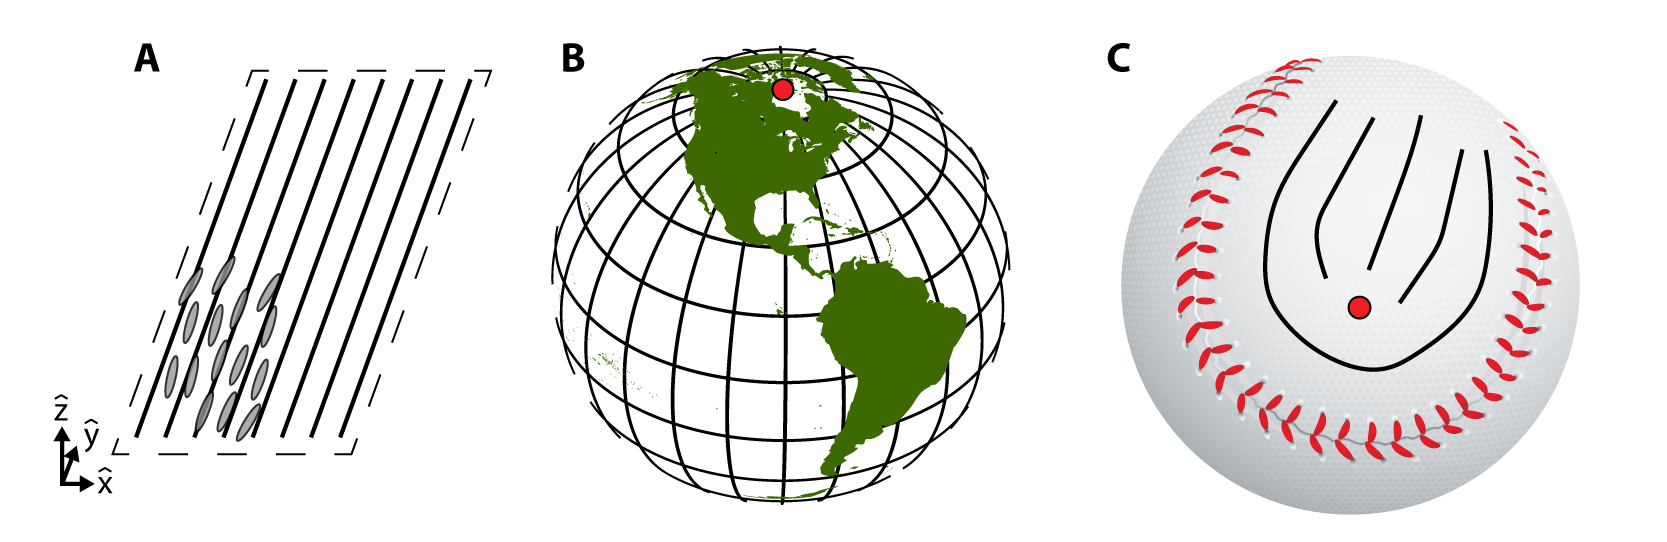
\includegraphics{figures/C1/Ch1-Figs_RodsPlane.png}
  \caption{Packing rods in two dimensions.
  (A-C), Rod-like particles preferentially align along a commmon axis, given by the black lines.
  (A) On a plane, the alignment can be homogeneous everywhere.
  (B,C) On a sphere, there must be singularities (${\color{red} \bullet}$) in the alignment directions, as shown for alighment directions along (B) the latitude or longitude lines on a globe and an alignment direction along (C) the stitching on a baseball.
  Note that there while only one singularity is visible in (B,C), there are 2 singularities in (B) and 4 in (C).}\label{f:1-RodsPlane}
\end{figure}

To formally relate the topology of the sphere with the presence of singularities, we need a few topological notions.
The sphere is an example of a differentiable surface that is compact, has no boundary, and is orientable.
Compact surfaces must both be bounded and contain their limit points.
Here, the term ``bounded'' means the surface has some finite size and is distinct from whether or not the surface has a boundary.
The boundary of a surface is defined as the set of points that can be approached from both the interior and the exterior of the surface.
Finally, orientable surfaces have a defined normal vector everywhere.
For example, 2D Euclidean space, denoted as $\mathbb{R}^2$, is a surface but it is not bounded and thus it is not compact.
Given $\mathbf{r} \in \mathbb{R}^2$, the 2D open unit disc $|\mathbf{r}| < d$ is not compact since it does not contain the circle with radius $d$.
However, the 2D unit disc $|\mathbf{r}| \leq d$ satisfies both conditions and thus is compact.
In addition, we see that $|\mathbf{r}| \leq d$ has a boundary $\partial \mathbf{r}$ at $|\mathbf{r}| = d$, as $\partial \mathbf{r}$ can be approached by points in both the interior and the exterior of the disc.
We call compact surfaces without a boundary closed surfaces.
Finally, all of these examples are also orientable; it is trivial to define a consistent surface normal everywhere.
\begin{figure}
  \centering
  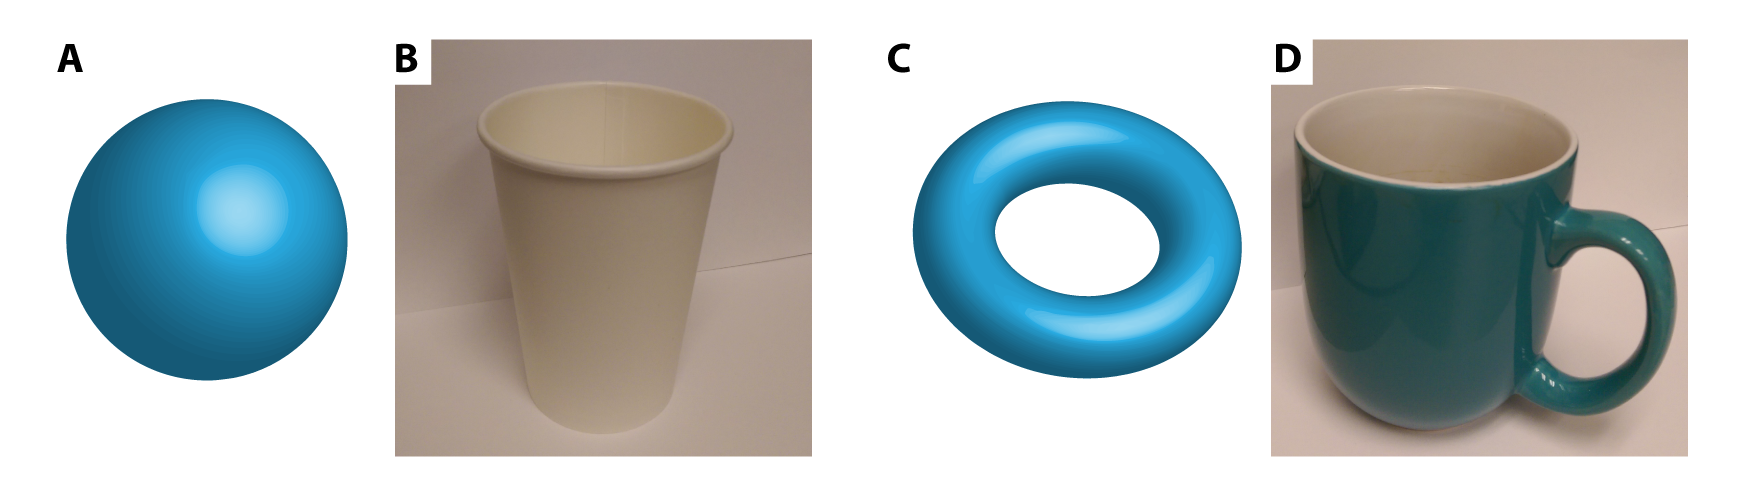
\includegraphics{figures/C1/Ch1-Figs_ChiObjects.png}
  \caption{Closed surfaces with the same Euler characteristic are homeomorphic. (A,B) Closed surfaces with no handle like a (A) sphere and a (B) cup can be continuously deformed into each other.
  (C,D) Closed surfaces with a single handle like a (C) torus and a (D) coffee mug can be continuously deformed into each other.
  However, the surfaces in (A,B) cannot be continuously deformed in the surfaces in (C,D) as the process of adding a handle breaks the surface.}\label{f:1-ChiObjects}
\end{figure}

We characterize the topological properties of a surface with its Euler characteristic, $\chi$, which we can calculate using the Gauss-Bonnet theorem.
For a closed surface, the theorem states that~\cite{RN23}:
\begin{equation}
  \chi = 2(1-g),\label{e:1-GB1}
\end{equation}
where $g$ is the genus, or number of handles, of the surface.
The Euler characteristic is a topological invariant --- continuously deforming a surface, i.e.\ under a homeomorphism, does not change its Euler characteristic.
A homeomorphism is continuous function with a continuous inverse that maps between topological spaces while preserving topological properties.
For example, a sphere has no handles, thus $g = 0$ and $\chi=2$.
Since a homeomorphism preserves the topological properties, any surface with $g=0$ is topologically equivalent, or homeomorphic, to the sphere, and therefore also has $\chi=2$.
For example, as pictured in Figure~\ref{f:1-ChiObjects}(A,B), a sphere is homeomorphic to a cup, as neither have handles.
Similarly, the torus and the coffee mug pictured in Figure~\ref{f:1-ChiObjects}(C,D), respectively, are also homeomorphic to each other.
However, the sphere [Figure~\ref{f:1-ChiObjects}(A)] and the torus [Figure~\ref{f:1-ChiObjects}(C)] are not homeomorphic as we cannot add a handle to the sphere without breaking its surface.

Thus, we can extend the statement, ``you cannot comb a hairy ball'' to, ``you cannot comb a hairy surface with $\chi=2$.''
In fact, any attempt to do so will necessarily result in the presence of singularities.
In an orientation field like a director field, singularities are called ``disclinations''.
We can characterize a disclination by how much the director rotates along a closed contour encircling the disclination.
For a contour $\partial A$ and the angle $\phi(\mathbf{r})$ parameterizing the director field, with $\mathbf{r}$ the position vectors of a point on the surface, we can calculate~\cite{RN23,RN153,RN203}:
\begin{equation}
  s = \frac{1}{2 \pi}\oint_{\partial A} \textrm{d}\mathbf{r} \cdot \nabla\phi(\mathbf{r}) = \frac{1}{2\pi} \oint_{\partial A} \textrm{d} \phi,\label{eq:1-topCharge}
\end{equation}
where $\textrm{d}\phi$ is an exact differential.
However, since $\phi$ is not a single-valued function, $\phi$ is not conservative and $s$ is not path independent.
If we map $\phi$ on $\partial A$ onto points on $\mathbb{S}^1$, the unit circle, we see that $s$ is the number of times the director field wraps the unit circle.
Since we cannot eliminate the enclosed disclination with continuous deformations of the director, disclinations are topological and $s$ is known as the winding number, or ``topological charge.''
Regardless of aligning rods along the latitudes or the longitudes on the Earth's globe, the director along a contour encircling either pole rotates by $2 \pi$, as depicted in Figure~\ref{f:1-TopCharge}(A).
Thus, both the north and the south poles have charge $s = +1$, bringing the total charge on the surface to $+2$.
The formal statement connecting a vector or director field on a closed surface with the topology of the surface is the Poincar\'e-Hopf theorem~\cite{RN23}:
\begin{equation}
  \sum\limits_{i = 1}^{N} s_i = \chi,\label{e:1-PH}
\end{equation}
where $N$ is the number of disclinations, each of topological charge $s_i$.

Thus, for nematic order, $s \in n/2$, where $n \in \mathbb{Z}$, the integers; however, for polar order, $s = n$.
For example, the defect structure in Figure~\ref{f:1-TopCharge}(B) has $s = +1/2$ and can exist in a nematic director field, where $\mathbf{n} = \mathbf{-n}$.
Attempting to construct such a disclination with a vector field, as illustrated by following the vectors as they go from blue to cyan along the red contour in Figure~\ref{f:1-TopCharge}(C), we see that we get a $\pi$-flip and the vector field is not continuous.
Note also that the Poincar\'e-Hopf Theorem only requires the total charge on the surface to be equal to $\chi$; we can construct a director or a vector field on a closed surface with any combination of defects so long as the total topological charge is equal to $\chi$.
\begin{figure}
  \centering
  
\includegraphics{figures/C1/Ch1-Figs_TopCharge.png}
  \caption{Topological charge of disclinations.
  (A), The director rotates by $2\pi$ along the contour enclosing the singularity (${\color{red} \bullet}$), giving $s = +1$ for both disclinations.
  (B) The director rotates by $\pi$ along the contour enclosing the singularity (${\color{red} \bullet}$), giving $s = +1/2$.
  (C) Attempting to construct an $s = +1/2$ disclination for a vector field results in a discontinuity in the vector field along the contour.
  This is seen by following the red contour as the vectors go from blue to cyan.}\label{f:1-TopCharge}
\end{figure}

Physical ordered systems constrained to a closed surface must then minimize their free energy while complying with the constraint imposed by the Poincar\'e-Hopf theorem.
For an orientationally ordered phase where the particles prefer to align parallel to each other, we can write the free energy as the cost of distorting the material from the homogeneously-aligned state.
In the continuum limit, this distortion free energy is a functional of the orientation field,
\begin{equation}
  F_d = \frac{1}{2} k_F \int \textrm{d}^2\mathbf{r} \, |\nabla \phi(\mathbf{r})|^2,\label{e:2-XY}
\end{equation}
where $k_F$ is the elastic constant governing the cost of distortion.
If we have polar order described by a vector field, then Eq.~\ref{e:2-XY} is the classical 2D X-Y model governing spins on a fixed lattice~\cite{RN175}; for nematic order, Eq.~\ref{e:2-XY} is the 2D Frank-Oseen free energy~\cite{RN61} in the 1-constant approximation~\cite{RN33}.

Nematics on a sphere were predicted~\cite{RN42,RN104,RN43} to minimize the free energy not with two $s=+1$ defects [Figure~\ref{f:1-RodsPlane}(B)] but with four $s=+1/2$ defects arranged on the vertices of a tetrahedron [Figure~\ref{f:1-RodsPlane}(C)].
Prior work in our group addressed this situation experimentally using glass-based microfluidic devices to fabricate double emulsions~\cite{RN272}, with a shell of nematic liquid crystal (NLC) between an inner water droplet and an outer water continuous phase~\cite{RN105,RN45}.
By decreasing the osmotic pressure in the outer continuous phase of the nematic shells, swelling of the inner droplet was induced.
This swelling decreased the thickness of the NLC shell to create an experimental realization of a 2D nematic on the surface of a sphere~\cite{RN45}.
In this thin shell limit, the four $s = +1/2$ defects arranged on the vertices of a tetrahedron was observed; see Figure~\ref{f:1-Shells}(A,B).
\begin{figure}
  \centering
  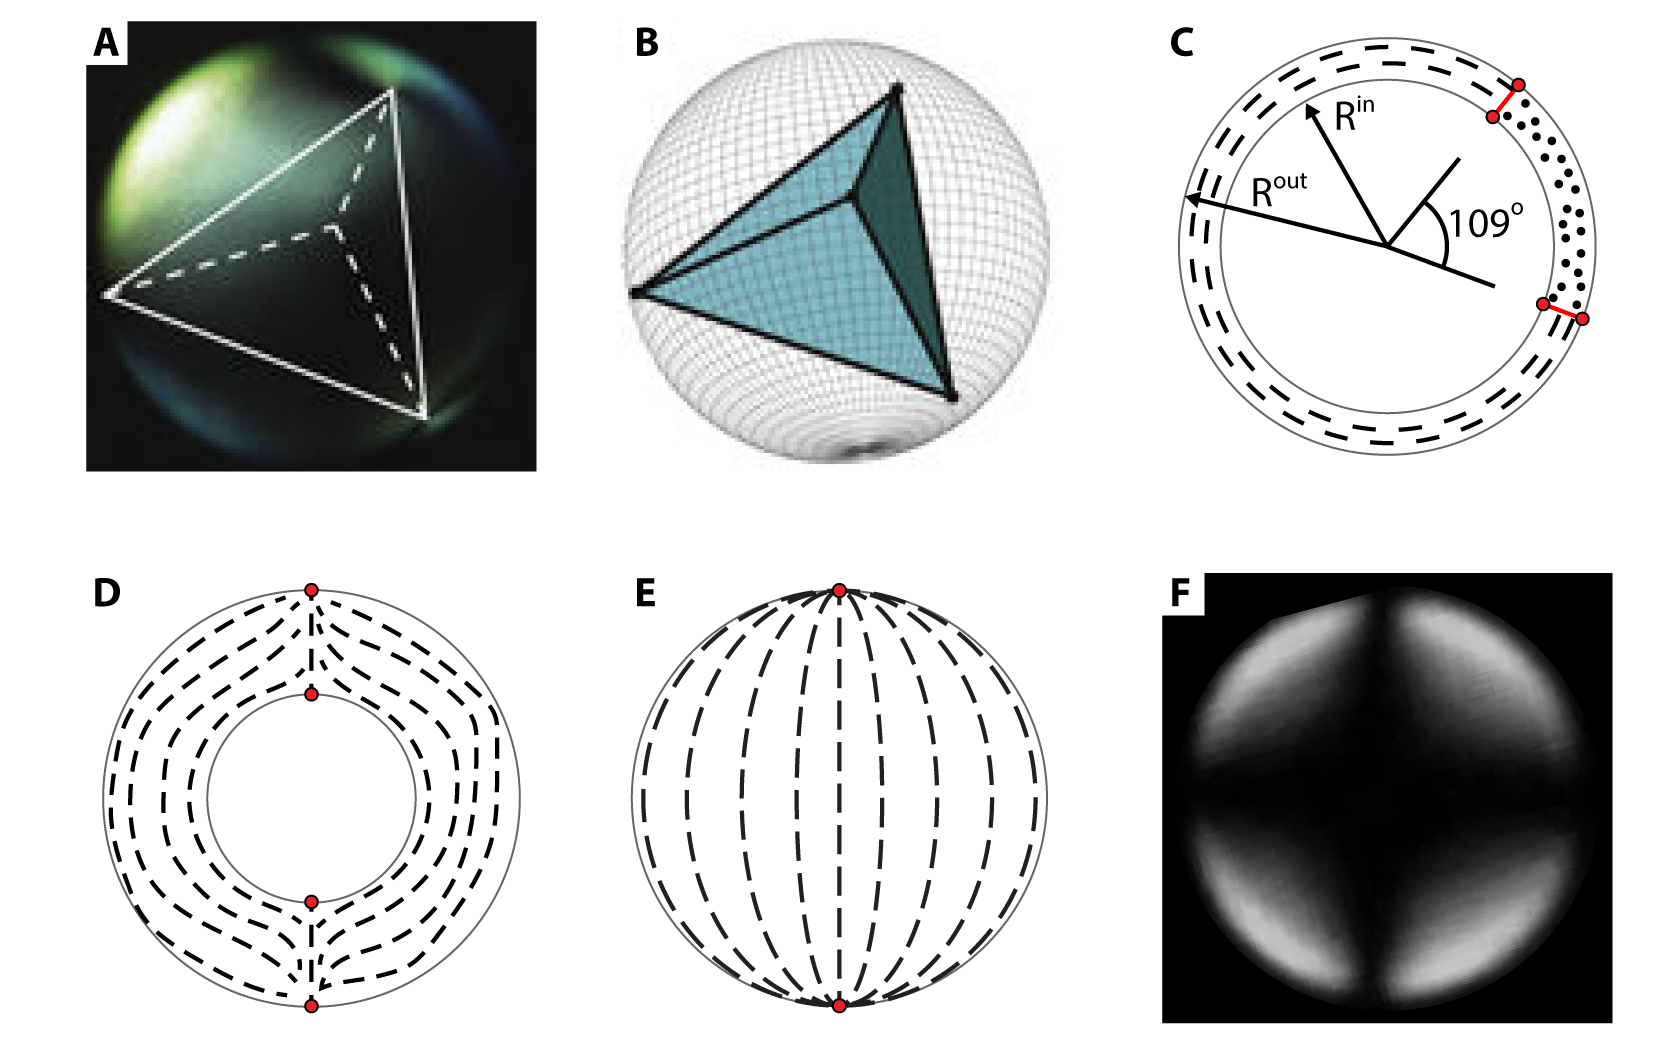
\includegraphics{figures/C1/Ch1-Figs_Shells.png}
  \caption{Shells of nematic liquid crystal.
  (A-C) Thin shells of NLC have four $s = +1/2$ defects, with an experimental crossed-polar image in (A), the tetrahedron highlighted in (B), and a cross-section schematically showing the director configuration in (C).
  The cross-section is of a great circle containing two $s = +1/2$ defects (${\color{red} \bullet}$) on both the inner and outer surface of the shell, with a red singular line connecting corresponding disclinations.
  The disclinations occupy the vertices of a tetrahedron and thus are separated by $109^{\circ}$ in the cross-section.
  (D) Cross-section of the director configuration in a thick shell. Here, the two $s = +1$ disclinations (${\color{red} \bullet}$) on each surface are no longer connected by a singular line.
  (E,F) As $R^{in}\rightarrow 0$, the thick shell becomes a bipolar droplet, with a cross-section of the director field in (E) and a corresponding crossed-polar image in (F).
  Images/Schematics in (A,B) reproduced from Ref.~\cite{RN105} with permission from Macmillan Publishers Ltd: \href{https://www.nature.com/nphys/}{Nature Physics}, copyright 2011.}\label{f:1-Shells}
\end{figure}

However, this tetrahedral arrangement of $s = +1/2$ defects only exists in thin enough shells, as characterized by the relative shell thickness $h' = (R^{out}-R^{in})/R^{out}$, with $R^{in}$ and $R^{out}$ the inner and outer radius of the nematic shell, as defined schematically in Figure~\ref{f:1-Shells}(C).
As $h'$ increases, the shell also becomes inhomogeneous due to density differences between the inner droplet and the NLC shell.
This thickness heterogeneity drives defects to the thinnest portion of the shell; this means that the $s = +1/2$ defects are no longer arranged in a tetrahedron.
In addition, as $h'$ increases, the shell can no longer be considered 2D.

The situation is now 3D and there are two spherical interfaces where the topological charge on the interface is constrained by the Poincar\'e-Hopf theorem, with a bulk region between the two surfaces filled with NLC.
Each $s = +1/2$ defect on the outer surface is connected to a corresponding $s = +1/2$ disclination on the inner surface via a singular line that propagates through the bulk.
This is depicted schematically in Figure~\ref{f:1-Shells}(C) for a great circle containing two $s = +1/2$ disclinations on each surface.
As $h'$ increases, so does the cost of each singular line.
Eventually, as $h'\gtrsim 1/2$, the cost of propagating the singular lines through the bulk is too great and pairs of $s = +1/2$ disclinations on each surface transition to one $s = +1$ disclination~\cite{RN105}, known as a boojum~\cite{RN273}.

Unlike the $s = +1/2$ defects, the corresponding boojums on the inner and outer surface are not connected by a singular line; instead, the director in the shell region ``escapes in the third dimension'' and acquires a component along the radius of the droplet, removing all the singularities in the bulk.
The increased energetic cost of a single boojum as compared to two $s = +1/2$ defects is compensated by the energetic decrease of removing the singular regions in the bulk of the shell.
This is depicted schematically for a two boojums on each surface for the special case of a homogeneous shell in Figure~\ref{f:1-Shells}(D).
For a heterogeneous thickness, the boojums will migrate towards the thinnest portion of the shell.
In addition, the shells are not restricted to either four $s = +1/2$ disclinations or two $s = +1$ boojums; our group also observed hybrid shells with two $s = +1/2$ disclinations and a single boojum.
For $h' = 1$, there is no inner water droplet and we have a single droplet of NLC in a continuous water phase, with the boojums on opposite poles.
This director arrangement is the classic bipolar configuration, with the director field and associated crossed polar image shown in Figure~\ref{f:1-Shells}(E,F), respectively.

This example shows that even if Eq.~\ref{e:2-XY} favors a homogeneous orientation field, corresponding to the zero energy configuration, sometimes distortions are unavoidable due to the topological constraints imposed by the surface.
However, ordered materials are also sensitive to the local geometry.
For example, consider once more rods packed on a plane with a homogeneous director field, as shown schematically in Figure~\ref{f:1-ParallelTransport}(A).
If we change the geometry and introduce a hemispherical ``bump'' in the plane, as illustrated in Figure~\ref{f:1-ParallelTransport}(B), evenly-spaced director lines on the plane do not maintain their spacing on the bump.
Thus, we no longer have a homogeneous director everywhere on the surface.
This inability to maintain the preferred local order due to the geometry of the surface is called ``geometrical frustration''.
Geometrical frustration is also commonly seen in magnetic systems.
For example, it is impossible to have a triangular antiferromagnetic lattice; the topology of the lattice frustrates the local antiferromagnetic order, as illustrated schematically in Figure~\ref{f:1-ParallelTransport}(D).
\begin{figure}
  \centering
  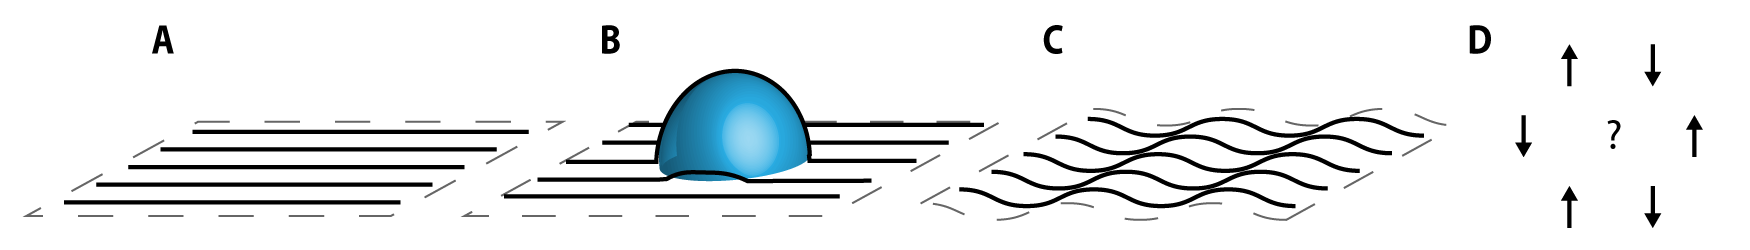
\includegraphics{figures/C1/Ch1-Figs_ParallelTransport.png}
  \caption{Geometrical frustration in nematics and in magnetism.
  (A), A flat plane can support a homogeneous director field, indicated by the black lines.
  (B), Adding a hemisphere to the plane disrupts the homogeneous state, the Gaussian curvature of the hemisphere makes a distortion-free state impossible.
  (C), Modulating the surface with a sine wave adds mean curvature but not Gaussian curvature to the surface; the homogeneous state on the surface is still possible.
  (D), Geometrical frustration in magnetism. Perfect antiferromagnetic order cannot exist on a triangular lattice.}\label{f:1-ParallelTransport}
\end{figure}

An important aspect of the local geometry of a surface is its curvature; consider a curve constrained to lie in $\mathbb{R}^2$, $\mathbf{r}(s)$, with $s$ the arclength parameter.
Such an example of a planar curve is drawn schematically in Figure~\ref{f:1-Curvature}(A).
The unit tangent to the curve at $s$ is given by $\mathbf{T}(s) = \textrm{d} \mathbf{r}(s)/\textrm{d}s = \mathbf{r}'(s)$, and the local curvature $\kappa(s)$ by $\mathbf{k}(s)\kappa(s) = \mathbf{T}'(s) = \mathbf{r}''(s) $, with $\mathbf{k}(s)$ the unit normal vector to the curve [see Figure~\ref{f:1-Curvature}(A)].
$\kappa(s) = 1/R(s)$, where $R(s)$ is the radius of the osculating circle, or circle that best approximates $\mathbf{r}(s)$ at $s$.
This radius is commonly known as the ``radius of curvature'' at $s$.
The sign of the curvature relates to the direction $\mathbf{k}$ rotates as $s$ increases: if $\mathbf{k}$ rotates counterclockwise, then $\kappa > 0$, while if $\mathbf{k}$ rotates clockwise, $\kappa < 0$.
The osculating circles and associated radii of curvature are drawn in blue and red in Figure~\ref{f:1-Curvature}(A) for a point with negative curvature and a point with positive curvature.

Now consider a 2D orientable surface given by $\mathbf{R}(u^1,u^2) \in \mathbb{R}^3$, with $(u^1,u^2) \in U \subset \mathbb{R}^2$ local coordinates on the surface, with $U$ a local coordinate patch.
We define a normal section at a point $\mathbf{r} \in U$ on the surface as the planar curve resulting from the intersection between the surface and a plane containing.
Since the orientation of the plane is not unique, there are infinitely many planes that can contain $\mathbf{k}(\mathbf{r})$, and therefore infinitely many normal sections at a given point $\mathbf{r}$.
The curvature of a given normal section at $\mathbf{r}$ is called the normal curvature.
A normal section, the plane containing $\mathbf{k}$, and the osculating circle whose $R$ determines the normal curvature $\kappa(s)$ are drawn schematically for an example surface in Figure~\ref{f:1-Curvature}(B).
Among all possible normal curvatures at $\mathbf{r}$, there is always a maximum and minimum normal curvature, with the planes containing the associated normal sections orthogonal to each other~\cite{RN35}.
These two curvatures are the principle curvatures at $\mathbf{r}$, $\kappa_1 (\mathbf{r})$ and $\kappa_2(\mathbf{r})$, and their associated tangent vectors at $\mathbf{r}$ are the principal directions; these directions and curvatures are drawn schematically for an example surface in Figure~\ref{f:1-Curvature}(C).
For $\kappa_1$ and $\kappa_2$, we define two important quantities: the Gaussian curvature $K  = \kappa_1 \kappa_2$ and the mean curvature $H = (1/2) (\kappa_1+\kappa_2)$.

We now see that adding the hemispherical bump to the plane, which has $K = H = 0$ everywhere, changes the geometry by adding both non-zero mean and Gaussian curvature.
However, it is the Gaussian curvature and not the mean curvature that is responsible for geometrical frustration.
This can be seen after modulating the flat plane with a sine wave in one direction, as shown in Figure~\ref{f:1-ParallelTransport}(C).
In this case, $K=0$ everywhere while $H$ changes throughout the surface.
Despite the fact that $H \neq 0$ everywhere, we can still maintain a homogeneous director field, in contrast to our example surface with $K \neq 0$ at the bump [Figure~\ref{f:1-ParallelTransport}(B)].
This is a reflection of the fact that Gaussian curvature is a property of the surface alone, that is, it is an intrinsic curvature.
We can determine the Gaussian curvature of a surface without knowing anything about the space the surface is embedded in.
In contrast, determining the mean, or extrinsic, curvature of a surface requires knowledge of the space the surface is embedded in.

Revisiting the Euler characteristic, we can rewrite the Gauss-Bonnet theorem for a differentiable closed surface as,
\begin{equation}
  \chi = \frac{1}{2 \pi} \int \, K \textrm{d}^2\mathbf{r} = 2(1-g)\label{e:1-GB2}.
\end{equation}
It is evident from Eq.~\ref{e:1-GB2} that the Gaussian curvature provides the connection between the local geometry and the topology of a closed surface.
This is a very important fact.
Even though $K$ is a property of the local geometry, integrating $K$ over a closed surface yields a topological invariant.
\begin{figure}
  \centering
  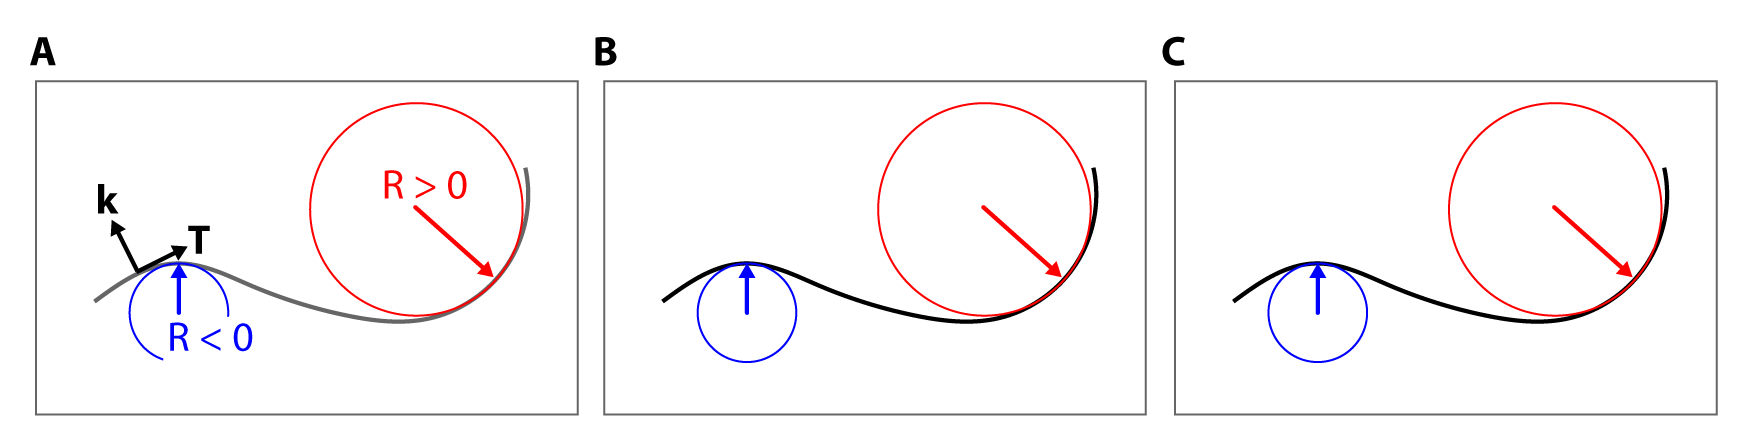
\includegraphics{figures/C1/Ch1-Figs_Curvature.png}
  \caption{Planar and surface curvature.
  (A), A planar curve with unit tangent vector $\mathbf{T}$ and unit normal vector $\mathbf{k}$. The osculating circles and associated radii of curvature are given for two points on the curve; the negative curvature is in blue and the positive curvature in red.
  (B), A normal section of a saddle-surface at a point corresponds to a planar curve, with the curve drawn in dark gray and the plane containing the curve indicated in transparent gray.
  The osculating circle and radius of curvature at the point of interest are drawn in blue.
  (C), The principal curvatures $\kappa_1$ and $\kappa_2$ at the point of interest on the surface from (B) are the maximum and minimum normal curvatures and are always in orthogonal directions. Here these directions are highlighted with the red and blue contours on the surface.}\label{f:1-Curvature}
\end{figure}

The connection between $K$ and the geometrical frustration is explicitly stated through the coupling of $K$ to the free energy of an orientationally ordered phase confined to a surface.
Considering the topological charge density,
\begin{equation}
  \rho(\mathbf{r}) = 2 \pi \sum\limits_i s_{i}\delta(\mathbf{r} - \mathbf{r}_{i}),\label{e:1-ChargeDens}
\end{equation}
due to disclinations indexed by $i$ possessing charge $s_{i}$ and position $\mathbf{r}_{i}$, where $\delta(\mathbf{r} - \mathbf{r}_{i})$ is the Dirac delta, we can express Eq~\ref{e:2-XY} as~\cite{RN42,RN175,RN17}:
\begin{equation}
  F_d = -\frac{1}{2} k_f \int \textrm{d}^2\mathbf{r} \, \textrm{d}^2\mathbf{r}' \, G_L(\mathbf{r},\mathbf{r}') [\rho(\mathbf{r})-K(\mathbf{r})] [\rho(\mathbf{r}')-K(\mathbf{r}')],\label{e:1-TopTheoryofDefects}
\end{equation}
where $G_L$ is the Green's function of the Laplace-Beltrami operator, the standard Laplacian operator generalized to curved space~\cite{RN17}.
Since $G_L$ has the form of the Coulomb potential for a unit point charge, Eq.~\ref{e:1-TopTheoryofDefects} is identical to the Coulomb energy of a plasma with charge density $\rho$ in a background of charge density $-K$~\cite{RN17}.
Thus, we see that topological defects can be treated as charged particles that couple to the surface via a background charge provided by the Gaussian curvature of the surface.

To investigate the role of curvature on ordered materials, we need to consider a space with varying Gaussian curvature and ideally, a space including Gaussian curvature of different sign.
While there have been new discoveries as a result of examining defect structures on spheres~\cite{RN106,RN26,RN110,RN76,RN101,RN165}, including prior work with spherical nematic shells~\cite{RN45,RN105}, the Gaussian curvature and therefore the background topological charge density is constant in these cases.
As a result, the impact of curvature only enters through the sphere radius.
This is borne out in both the size-dependent onset of grain-boundary scars in colloidal crystals on the surface of emulsion drops~\cite{RN26,RN110}, and in the fact that the positions of the four $s = +1/2$ defects in nematic shells are entirely determined by the defect-defect interactions, with the underlying geometry playing no role~\cite{RN45}.

The simplest closed surface with regions of both $K>0$ and $K<0$ is the torus [Figure~\ref{f:1-ChiObjects}(C)], which has $g = 1$ and thus $\chi = 0$.
In addition, we see that not only does a torus have sphere-like positive Gaussian curvature on its outer region and saddle-like negative Gaussian curvature on its inner region, but according to Eq~\ref{e:1-GB2}, the integrated Gaussian curvature over an entire torus must vanish.
Similarly, by Eq.~\ref{e:1-PH}, an orientationally ordered material on the surface of a torus must have vanishing topological charge and thus can support a defect-free configuration.

Prior work in our group investigated nematic order inside a torus using toroidal droplets made from a NLC, with the nematic director constrained to lie parallel to the interface between the toroidal droplet and the outer continuous medium~\cite{RN24,RN47}.
The varying curvature of the torus yielded doubly-twisted ground state with no defects~\cite{RN24}, as drawn for both a right-handed twist and a left-handed twist in Figure~\ref{f:1-Torus}(A,B), respectively.
The double-twist is directly related to a director distortion called saddle-splay, which favors the director in the plane of the surface aligning along the smallest principal curvature~\cite{RN59}.
We found that the amount of twist in the ground state can be controlled by the aspect ratio, or slenderness of the torus $\xi = R_0/a$, with $R_0$ the radius of the central circle of the torus and $a$ the tube radius of the torus, as defined in the top view schematic in Figure~\ref{f:1-Torus}(C).
In addition, as seen by the possibility of having either a right-handed or a left-handed twist, this doubly-twisted state manifests itself through a spontaneous reflection symmetry breaking, where the form of the free energy resembles that of the Landau theory of magnetism.
This analogy is exact for a linear twist in the cylindrical limit, where $\xi \rightarrow \infty$~\cite{RN293}.
These results clearly illustrate how confinement within surfaces of non-constant $K$ can affect the ground state of a system, even in the absence of defects.
\begin{figure}
  \centering
  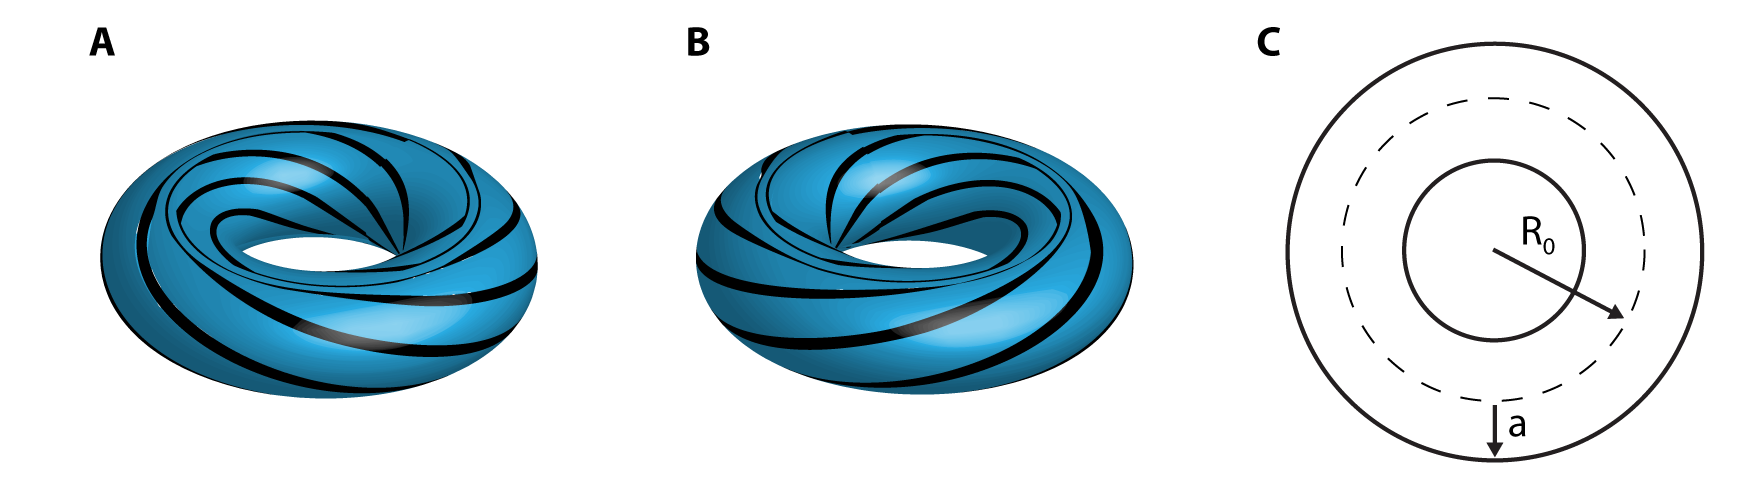
\includegraphics{figures/C1/Ch1-Figs_Torus.png}
  \caption{Doubly-twisted tori.
  (A,B), Schematics showing a (A) right-handed and (B) left-handed double-twist.
  (C), Schematic defining the central ring radius $R_0$ and tube radius $a$ in a torus.}\label{f:1-Torus}
\end{figure}

There are, however, 3D nematic fields with defects in their bulk.
For example, consider a nematic inside a volume with the director at the surface of the volume of the perpendicular to the surface.
We call this homeotropic anchoring.
If the volume is a sphere, we then see that irrespective of how we arrange the director in the bulk, there must be an irreducible singularity.
Bulk singularities that are points are known as hedgehogs and are characterized by their hedgehog charge,
\begin{equation}
  q = \frac{1}{4 \pi} \int_{\mathbb{S}^2} \textrm{d}\theta \: \textrm{d}\phi \: \mathbf{n} \cdot \left [ \partial_{\theta} \mathbf{n} \times \partial_{\phi} \mathbf{n} \right ],\label{e:1-HedgehogCharge}
\end{equation}
where the integral is taken over a topologically spherical surface enclosing the defect, and $\theta$ and $\phi$ are, respectively, the polar and azimuthal angles on that surface~\cite{RN153}.
In this case, instead of counting the number of times the director wraps around $\mathbb{S}^1$, as we did for the topological charge, we consider the orientation of $\mathbf{n}$ on the spherical surface enclosing the defect mapped to $\mathbb{S}^2$, the unit sphere.
The integrand in Eq.~\ref{e:1-HedgehogCharge} is the Jacobian from the director on the topologically spherical surface in real space to $\mathbb{S}^2$; it tells us how much area on $\mathbb{S}^2$ is covered by $\mathbf{n}$ on the surface enclosing the defect.
Thus, the hedgehog charge is then the number of times the orientations of $\mathbf{n}$ cover $\mathbb{S}^2$~\cite{RN153}.
Therefore, confining a NLC to a volume that is topologically spherical with homeotropic boundary conditions must yield a total ``hedgehog charge'' $|q|=1$.

In this Thesis, we investigate the role of geometry in the interplay between order and confinement.
In Chapter 2, we begin with an introduction to the theory of nematic liquid crystals.
Then, in Chapter 3, we consider nematic order on the surface of a torus.
This is different from previous studies where the NLC filled the torus~\cite{RN24,RN274,RN44}.
Due to the difficulty of creating a thin, stable, toroidal shell of a NLC, we use a polymeric nematic that self-assembles at the interface between two immiscible liquids.
Importantly, with this system we can generate stable toroidal droplets as in our previous work, and investigate 2D nematic order on a toroidal surface.
In addition, the nematic is active, meaning that the individual constituent particles have their own source of internal energy.
The activity then drives the nematic out of equilibrium at the individual particle level, generally causing the generation of pairs of $s = \pm 1/2$ defects that are constantly in motion and constantly being created and annihilated.
Even though we have an inherently nonequilibrium material, we find that predictions built upon Eq.~\ref{e:1-TopTheoryofDefects} hold and that adding activity to order qualitatively resembles bringing an equilibrium system to the high temperature limit.
However, there are significant differences with equilibrium nematics, which we will highlight.

In Chapter 4, we consider a NLC confined to toroidal droplets with homeotropic anchoring.
With the director constrained to lie perpendicular to the surface, the saddle-splay distortion does not affect the free energy minimization.
However, we still find a twisted ground-state configuration, where the amount of twist depends on $\xi$, eventually disappearing as $\xi \rightarrow \infty$.
Experiments with NLC confined to straight and bent cylindrical capillaries under homeotropic boundary conditions reveal that the twist is a response to the additional curvature induced when deforming a cylinder of homeotropic nematic into a torus.
This is new; prior experiments in cylinders found a twisted ground state only when NLC that favor twist distortions were used.
In our case, the confining geometry induces twist even in NLC that do not preferentially favor twist distortions.

In Chapter 5, we return to a spherical topology, confining NLC to a capillary bridge with homeotropic anchoring to study the influence of confinement shape on defect type.
We generate waist-shaped and barrel-shaped bridges and find that waist-shaped bridges contain hyperbolic defects with negative hedgehog charge while barrel-shaped bridge contain radial defects with positive hedgehog charge.
In addition, we find that the ratio of the bridge height to its width determines whether or not the singularity is a ring defect or a hedgehog.

In Chapter 6, we summarize, conclude, and present results that open the door to future work that builds on this Thesis.


%%%%%%%%%%%%%%%%
% Chapter 2
%%%%%%%%%%%%%%%%

%!TEX root = thesis.tex
\chapter{Fundamentals of nematic liquid crystals}\label{c:2}

\section{Local order and defects}
Uniaxial nematic liquid crystals are an ordered phase resulting from breaking the continuous rotational symmetry of a collection of anisotropic, typically rod-like or plate-like, particles~\cite{RN33}.
As either the concentration of the particles is increased~\cite{RN204} or the temperature of the system is decreased~\cite{RN202}, there is a point where a phase transition happens and the system breaks continuous rotational symmetry and develops order.
The order is characterized by a spontaneously chosen preferred direction or axis; rod-like particles prefer to have their long axis aligned along this direction and plate-like particles prefer to have their short axis along this direction~\cite{RN33,RN175}.

Note that the system still possesses continuous rotational symmetry about the preferred alignment direction as well as continuous translational symmetry in  all directions.
This is illustrated with rod-like particles in Figure~\ref{f:2-NematicSym}.
In panel (A), the system is isotropic and there is no preferred alignment direction.
In contrast, in panels (B) and (C), the rods now align along a preferred direction denoted by $\mathbf{n}$ and called the director.
As a result, in Figure~\ref{f:2-NematicSym}(B) and Figure~\ref{f:2-NematicSym}(C), the system has broken continuous rotational symmetry about the two axes orthogonal to $\mathbf{n}$.
Note that even though in Figure~\ref{f:2-NematicSym}(C) the rods align more strongly along $\mathbf{n}$ than the rods in Figure~\ref{f:2-NematicSym}(B), the system possesses the same symmetry in both situations.

Regardless of the rotational symmetry of the system, the system never breaks translational symmetry.
This can be seen in Figure~\ref{f:2-NematicSym}(D), where we show the centers of mass of the rods for all the cases in Figure~\ref{f:2-NematicSym}(A--C), illustrating that there is no positional order and the system still possesses continuous translational symmetry.
If the concentration of the particles were further increased or the temperature were further decreased, the system would eventually break translational symmetry and the nematic phase would transition to a crystalline phase, with three broken continuous translational symmetries~\cite{RN33}.
Hence, the liquid-crystalline nematic phase is an intermediate ``mesophase'' that possesses the continuous translational symmetries of the isotropic ``liquid phase'' as well as some of the broken rotational symmetries of the ``crystalline'' phase.

We briefly mention that nematics can be biaxial instead of uniaxial.
Here, the constituent particles are bar-like such that there is no longer a single axis of symmetry that can characterize the particle geometry~\cite{RN33,RN175}.
Instead, we would need to define two axes, hence the name biaxial.
However, in this Thesis, we will focus only on uniaxial NLC whose constituent particles are rod-like.

\begin{figure}[h]
  \centering
  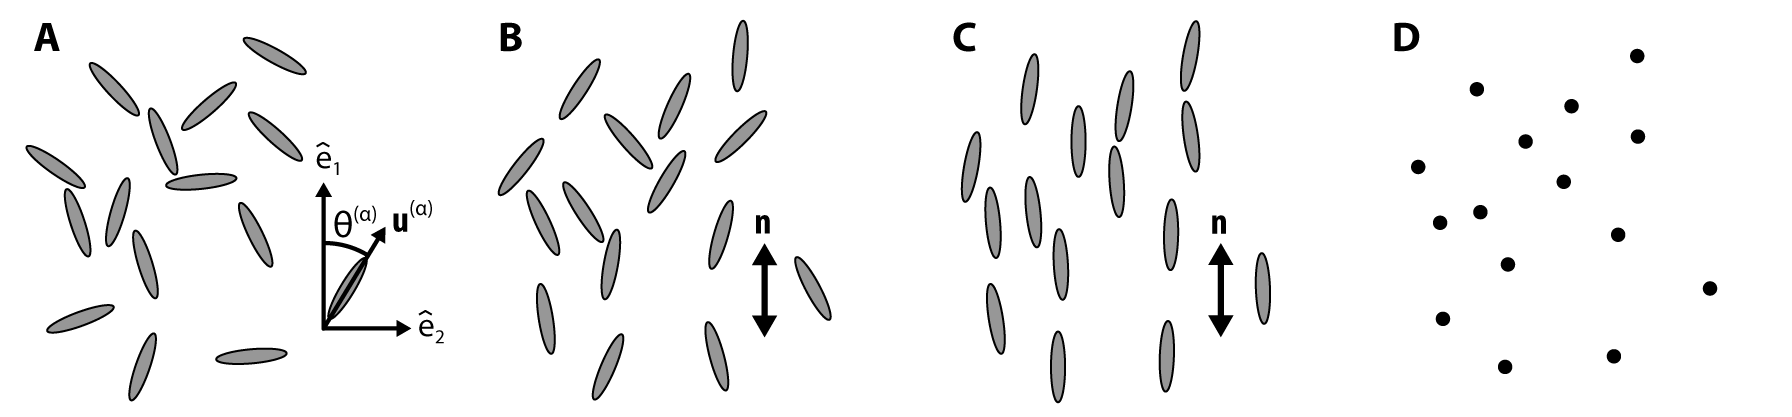
\includegraphics{figures/C2/Ch2-Figs_NematicSym.png}
  \caption{ Symmetries in nematic phase. (A), A collection of rod-like particles in the isotropic phase.
  The orientation of the rod with index $\alpha$ is given by the angle $\mathbf{u}^{\alpha}$, defined schematically in the image.
  (B), The rods from (A) in the nematic phase.
  The rods are preferentially but weakly aligned along the director $\mathbf{n}$, denoted in the panel.
  (C), The rods from (A,B) in the nematic phase. Here, the rods are strongly aligned along $\mathbf{n}$, denoted in the panel.
  (D), The positions of the center of mass of the rods in (A--C), highlighting the continuous translational symmetry of the rods.}\label{f:2-NematicSym}
\end{figure}

\subsection{The director and the order parameter}
Given a group of rods, we want to determine if the system is in the isotropic or the nematic phase, in addition to finding the director, $\mathbf{n}$, provided that the rods are in the nematic phase.
Since we have a collection of rods with no specified head nor tail, the director possesses inversion symmetry, where $\mathbf{n}$ and $-\mathbf{n}$ describe the same physical state.
In addition, we take the director to have unit length, $\mathbf{n}\cdot\mathbf{n} = 1$.
Thus, to indicate nematic order, we need an order parameter that goes to $0$ in the isotropic phase, is nonzero in the nematic phase, and describes the broken symmetry~\cite{RN33,RN175}.
We will first derive this quantity for a collection of rods laying in a 2D plane and then generalize to rods in 3D.
Let a 2D collection of rods laying in a plane be indexed by $\alpha = 1,2,\dots, N$, such that the orientation of a given rod can be specified with the unit vector $\mathbf{u}^{(\alpha)} = u^{(\alpha)}_i\hat{e}_i$, as seen in Figure~\ref{f:2-NematicSym}(A), where we use the Einstein summation convention to sum over repeated indices and $\{\hat{e}_1,\hat{e}_2  \}$ is the standard basis in $\mathbb{R}^2$.
Note that due to the inversion symmetry of the nematic phase $\langle \mathbf{u}^{(\alpha)}\rangle_{\alpha} = 0$, where $\langle \cdot \rangle_{\alpha}$ represents an ensemble average over all $\alpha$.
Thus, to accommodate the inversion symmetry of $\mathbf{u}^{(\alpha)}$, we will construct a symmetric rank-2 tensor from $\mathbf{u}^{(\alpha)}$.
Let:
\begin{equation}
  \mathbf{Q} = \left \langle \mathbf{u}^{(\alpha)} \otimes \mathbf{u}^{(\alpha)} - \frac{1}{2} \mathbb{1} \right \rangle_{\alpha},\label{e:2-2DOrderRaw}
\end{equation}
with $\otimes$ the outer product.
Now, $\textrm{tr}\big \{ \mathbf{Q} \big \} = \langle \mathbf{u}^{(\alpha)} \cdot \mathbf{u}^{(\alpha)} - 1 \rangle_{\alpha} = 0$, making $\mathbf{Q}$ traceless~\cite{RN33,RN175}.
We need $\mathbf{Q}$ to be traceless if we wish to use $\mathbf{Q}$ as an order parameter with $Q_{ij} = 0$ in the isotropic phase.

To determine the director, we need to diagonalize $\mathbf{Q}$.
Without loss of generality, we choose a new orthonormal basis in the plane, $\{ \hat{e}_1', \hat{e}_2' \}$.
The transformation from the unprimed to the primed basis is given by the matrix $V_{ij} = \hat{e}'_i \cdot \hat{e}_j$.
Note that $\mathbf{V}^T \mathbf{V} = V_{ij}V_{jk} =  \mathbb{1}$, implying that $\mathbf{V}^T = \mathbf{V}^{-1}$, and $\mathbf{V}$ is orthogonal.
We then have:
\begin{align}
  \mathbf{Q}' = \mathbf{V} \mathbf{Q} \mathbf{V}^T &=
  \bigg \langle \big ( \mathbf{V} \mathbf{u}^{(\alpha)} \big ) \otimes \big ( \mathbf{V} \mathbf{u}^{(\alpha)} \big )\bigg \rangle_{\alpha}  - \frac{1}{2} \mathbb{1} \nonumber \\ & =
  \begin{pmatrix}
    \langle \cos^2 \theta'^{(\alpha)}\rangle_{\alpha} - 1/2 & \langle \sin \theta'^{(\alpha)} \cos \theta'^{(\alpha)} \rangle_{\alpha} \\
    \langle \sin \theta'^{(\alpha)} \cos \theta'^{(\alpha)} \rangle_{\alpha} & \langle \sin^2 \theta'^{(\alpha)} \rangle_{\alpha} - 1/2
  \end{pmatrix},\label{e:2-2DOrderRot}
\end{align}
where $\cos \theta'^{(\alpha)} = \mathbf{u}^{(\alpha)} \cdot \hat{e}_1'$ and $\sin \theta'^{(\alpha)} = \mathbf{u}^{(\alpha)} \cdot \hat{e}_2'$.

Since $\mathbf{Q}$ is symmetric, we can always find a basis of eigenvectors where $\mathbf{Q}'$ is diagonal.
Choose the $\hat{e}'_i$ to be the eigenvectors of $\mathbf{Q}$.
This implies $ \mathbf{V} \mathbf{Q} \mathbf{V}^T$ must be diagonal such that $\langle \sin \theta'^{(\alpha)} \cos \theta'^{(\alpha)} \rangle_{\alpha} = \langle \sin (2 \theta'^{(\alpha)}) \rangle_{\alpha} = 0$.
This can occur in two instances.
First, if we choose the collection of rods to be randomly oriented as in the isotropic phase, $\langle \sin (2 \theta'^{(\alpha)}) \rangle_{\alpha} = 0$ as sine is an odd function.
However, in this case we also have $\langle \cos^2 \theta'^{(\alpha)}\rangle_{\alpha} - 1/2 = \langle \sin^2 \theta'^{(\alpha)}\rangle_{\alpha} - 1/2 = 0$, and thus $\mathbf{Q} = 0$.
This first situation simply shows the correct behavior in the isotropic phase.
The second situation is the one we are seeking.
For $\langle \sin (2 \theta'^{(\alpha)}) \rangle_{\alpha}$ to be $0$, the collection of rods must on average point along $\hat{e}'_i$, implying that $\theta'^{(\alpha)} \approx 0 \textrm{ or } \pi/2$.
This further indicates that $\mathbf{n}$ is either along $\hat{e}_1'$ or along $\hat{e}_2'$, the eigenvectors of $\mathbf{Q}$.

We now take Eq.~\ref{e:2-2DOrderRot} and write it assuming the collection of rods on average points along $\hat{e}'_1$, hence $\mathbf{n} = \hat{e}_1'$.
This yields:
\begin{equation}
  \mathbf{V} \mathbf{Q} \mathbf{V}^T =
  \begin{pmatrix}
    \langle \cos^2 \theta'^{(\alpha)}\rangle_{\alpha} - 1/2 & 0 \\
    0 & \langle \sin^2 \theta'^{(\alpha)} \rangle_{\alpha} - 1/2
  \end{pmatrix} =
  \begin{pmatrix}
    S/2 & 0 \\
    0 & -S/2
  \end{pmatrix},\label{e:2-2DOrderDiagBig}
\end{equation}
where $S = 2 \langle \cos^2 \theta'^{(\alpha)} \rangle_{\alpha} - 1$.
From Eq.~\ref{e:2-2DOrderDiagBig}, we find that the eigenvalue associated to the eigenvector $\hat{e}_1'$ is $S/2$, while for the eigenvector $\hat{e}_2'$ the eigenvalue is $-S/2$.
Since we specified that the rods prefer to align along $\hat{e}_1'$, we see that $\mathbf{n}$ is the eigenvector that corresponds to the largest eigenvalue of $\mathbf{Q}$.
S is often called the scalar order parameter and denotes how well-aligned the system is~\cite{RN33}.
For example, if every rod was aligned along $\hat{e}_1'$ such that $\mathbf{u}^{(\alpha)} = \hat{e}'_1$, $S = 1$.
Similarly, if we again check the isotropic limit of a random collection of rods, we see that $S = 0$, as desired.
Returning to Figure~\ref{f:2-NematicSym}, we see that $S=0$ in Figure~\ref{f:2-NematicSym}(A), and that $0 < S\big[$Figure~\ref{f:2-NematicSym}(B)$\big] < S\big[$Figure~\ref{f:2-NematicSym}(C)$\big] < 1$.
Thus, $\mathbf{Q}$ serves as the tensor order parameter for a collection of rods, where the director corresponds to the eigenvector associated with the largest eigenvalue of $\mathbf{Q}$, and that eigenvalue gives $S$, the scalar order parameter~\cite{RN33,RN175}.

In terms of the director, we can now write $\mathbf{Q}$ in 2D as:
\begin{equation}
  \mathbf{Q} = S \left ( \mathbf{n} \otimes \mathbf{n} - \frac{1}{2}\mathbb{1} \right ).\label{e:2-2DOrderDiag}
\end{equation}
Generalizing to 3D, we have a similar expression for a collection of rods~\cite{RN33}:
\begin{equation}
  \mathbf{Q} =  \left \langle \mathbf{u}^{(\alpha)} \otimes \mathbf{u}^{(\alpha)} - \frac{1}{3} \mathbb{1} \right \rangle_{\alpha},\label{e:2-3DOrderRaw}
\end{equation}
that can be written in terms of the director as:
\begin{equation}
  \mathbf{Q} = S \left ( \mathbf{n} \otimes \mathbf{n} - \frac{1}{3}\mathbb{1} \right ),\label{e:2-3DOrderDiag}
\end{equation}
with $S = \frac{1}{2} \big \langle 3 \cos^2 \theta'^{(\alpha)}  - 1 \big  \rangle_{\alpha} = \big \langle P_2(\cos \theta'^{(\alpha)}) \big \rangle_{\alpha} $,
where again $\theta'^{\alpha} = \arccos (\mathbf{u}^{\alpha} \cdot \mathbf{n})$, and $P_2(\cdot)$ is the Legendre Polynomial of order 2~\cite{RN33,RN175}.
As in two dimensions, we take the eigenvector associated with the largest eigenvalue to be $\mathbf{n}$.
Thus, for a collection of rods, we can determine if the collection is nematic or isotropic and, if applicable, $\mathbf{n}$ by calculating $\mathbf{Q}$ according to Eqs.~\ref{e:2-2DOrderRaw} or~\ref{e:2-3DOrderRaw} and diagonalizing.


\subsection{Defects in a nematic}\label{c:2-defects}
While we briefly mentioned the dimensionality of defects and their associated classification schemes in Section~\ref{c:1}, here we take a deeper look and use homotopy theory as laid out in references~\cite{RN196,RN236,RN153} to introduce a more complete theory of defects in nematic materials.
Homotopy theory deals with classifying elements of topological spaces using a group structure; in this case, we will classify defects as members of the first and second homotopy groups.
As mentioned in Chapter~\ref{c:1}, defects in ordered media are defined generally as regions where the characteristic order of the phase is not satisfied.
In a nematic phase, defects are locations where $\mathbf{n}$ is undefined.
For a nematic in 3D, these locations can be $0$-dimensional ($0$D) (point defects), $1$-dimensional ($1$D) (line defects), or $2$D (wall defects).
General examples of defects with different dimensionality in 3D and 2D are drawn schematically in Figure~\ref{f:2-GenDef}.
Note that when a 3D defect structure depends only on 2 coordinates, as seen in the invariance along $\hat{z}$ in the wall and line defects in Figure~\ref{f:2-GenDef}, the director in the $xy$ plane appears as if we were in 2D.
For example, a wall in 3D is similar to a line in 2D and a line in 3D is similar to a point in 2D, as highlighted by the arrows in Figure~\ref{f:2-GenDef}.

However, while it is appealing to equate similar-looking structures in 2D and 3D, the additional possible director orientations in a 3D nematic mean that a 3D nematic is fundamentally different than a 2D nematic.
To characterize these differences as well as classify the defects themselves we turn to the homotopy theory of defects.
For clarity, we refer to Table~\ref{t:2-GroupTheory} for definitions of some useful concepts from group theory.\\
\begin{figure}[h]
  \centering
  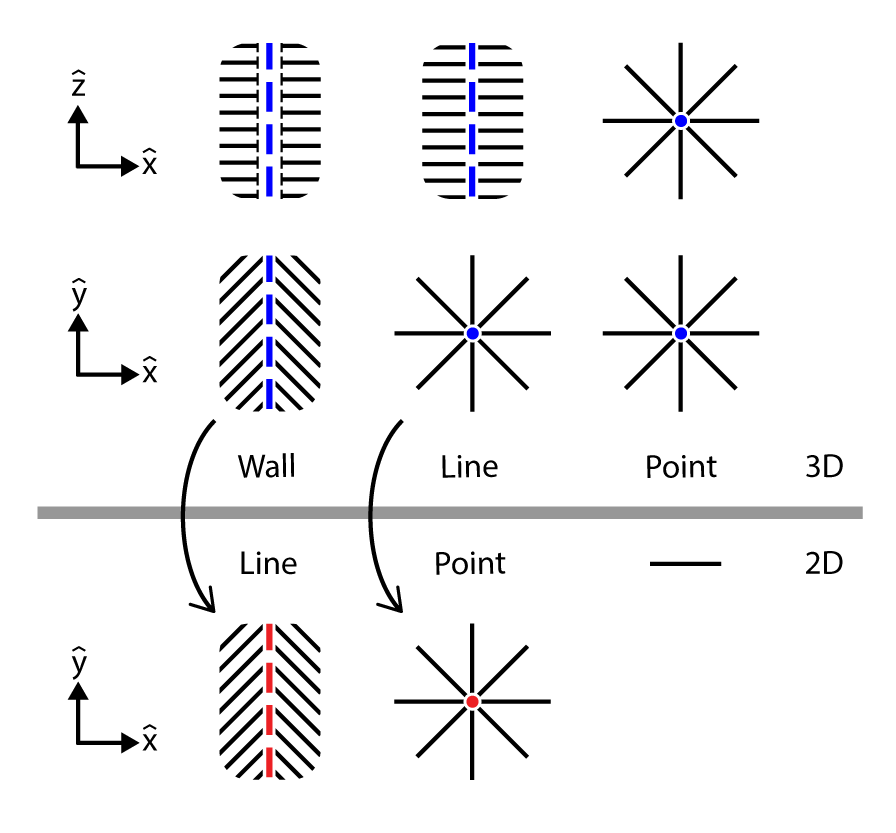
\includegraphics{figures/C2/Ch2-Figs_GenDef.png}
  \caption{Different types of defects in 3D and 2D.
  In 3D, there is the 2D wall defect, the 1D line defect, and the 0D point defect.
  Cross-sections of these three structures are shown schematically in the $xy$ plane and the $xz$ plane.
  The defects are marked with either a dot or a dashed line.
  The heads of the``nails'' in the $xz$ cross-section of the wall, point into the page.
  In 2D, a nematic can have 1D line defects and 0D point defects, where the singular region is highlighted with either a dashed line or a point.
  Note that the wall and line structures in 3D are invariant along the $\hat{z}$-direction.
  This invariance means that the $xy$ cross-section of the wall and line structure in 3D map to the line and point structure in 2D, as shown by the arrows in the schematic.}\label{f:2-GenDef}
\end{figure}

Consider a set of vectors in 2D such that their orientations can be described by a single angle.
We can map these vector orientations onto an \emph{order parameter space} given by the 1-sphere, $\mathbb{S}^1$, the unit circle in the plane, such that $\mathbb{S}^1$ describes all the possible orientations of the vectors.
If instead we consider a nematic, $\mathbb{S}^1$ is no longer an appropriate order parameter space as the orientations of $\mathbf{n}$ are periodic on the interval $[0,\pi)$ and not on the interval $[0,2 \pi)$.
Instead, for 2D nematics the order parameter space is $\mathbb{R}\mathbb{P}^1$, the real projective plane in 1D, which corresponds to $\mathbb{S}^1$ with antipodal points identified~\cite{RN196,RN153,RN236}.
This means that specifying the director along a contour in real space will determine a mapping to the order parameter space.

For example, consider both the purple contour and the red contour in the real space director schematic in Figure~\ref{f:2-2DMeas}(A) and their associated mappings to $\mathbb{R}\mathbb{P}^1$ in the schematic in Figure~\ref{f:2-2DMeas}(B,C).
Both contours are closed.
However, we see in Figure~\ref{f:2-2DMeas}(A) that the red contour encloses a singularity while the purple contour does not.
Similarly, we see that in the order parameter space in Figure~\ref{f:2-2DMeas}(B), the purple contour does not span $\mathbb{RP}^1$ and thus can be continuously deformed to a point in $\mathbb{R}\mathbb{P}^1$.
In contrast, the red contour in Figure~\ref{f:2-2DMeas}(C) spans $\mathbb{RP}^1$ and cannot be shrunken continuously to a point.
Thus, the presence of a singularity in the area bounded by the red contour in real space results in a nonzero winding number in the associated contour in the order parameter space.

In fact, it is easy to see that a mapping of the director along the blue contour in Figure~\ref{f:2-2DMeas}(D) will result in a contour in $\mathbb{R}\mathbb{P}^1$ that spans $\mathbb{RP}^1$ and goes in opposite direction to the red contour in  Figure~\ref{f:2-2DMeas}(C).
A mapping of the director to $\mathbb{R}\mathbb{P}^1$ along the green contour in Figure~\ref{f:2-2DMeas}(E) will result in a contour that wraps $\mathbb{R}\mathbb{P}^1$ twice in the same direction as the red contour.
Explicitly, we see that the defect structures in Figure~\ref{f:2-2DMeas}(A,D,E) all have different winding numbers in $\mathbb{R}\mathbb{P}^1$, and thus cannot be mapped onto each other with continuous deformations.
In the language of homotopy theory, we say that any two contours that can be continuously deformed into each other (i.e., via a homeomorphism) are homotopic~\cite{RN196}.
More generally, any contour in $\mathbb{R}\mathbb{P}^1$ with winding number $k$ is homotopic to any other contour in $\mathbb{R}\mathbb{P}^1$ with winding number $k$, and only to contours with winding number $k$~\cite{RN196,RN153,RN236}.
For example, note that as a single point in $\mathbb{R}\mathbb{P}^1$ corresponds to a homogeneous $\mathbf{n}$-field in real space, we see that the singularity-free director field with $k=0$ bounded by the purple contour in Figure~\ref{f:2-2DMeas}(A) is homotopic to the homogeneous state of any orientation, but is not homotopic to the director field with $k=1$ bounded by the red contour in Figure~\ref{f:2-2DMeas}(A).
Thus, contours with the same winding number form a homotopy class, where we can now start to think about categorizing the different homotopy classes of defects using a group structure.

While we could form the group using the winding numbers in $\mathbb{R}\mathbb{P}^1$ themselves, it is more common to use the winding number about $\mathbb{S}^1$ such that the winding number is equivalent to measuring the amount of director rotation around a contour in real space~\cite{RN23,RN153,RN203}.
Reproducing Eq.~\ref{eq:1-topCharge} from Chapter~\ref{c:1} for a director field parametrized by the angle $\phi(\mathbf{r})$, we characterize the defects with their winding number, $s$~\cite{RN153,RN236}:
\begin{equation}
  s = \frac{1}{2 \pi}\oint_{\partial A} \textrm{d}\mathbf{r} \cdot \nabla\phi(\mathbf{r}),\label{eq:2-topCharge}
\end{equation}
where $\partial A$ is the boundary of some area $A$ containing the defect and the integral is performed along the boundary keeping A to the left.
Since we have already established that the defects in a 2D nematic have integer winding numbers in $\mathbb{R}\mathbb{P}^1$, we see that $s = n/2$, with $n \in \mathbb{Z}$, giving us a discrete set of elements.
In addition, we know that winding numbers are additive~\cite{RN196}, such that combining the effect of multiple defects is commutative and associative.
The additivity can be seen in Figure~\ref{f:2-2DMeas}(F), where a contour surrounding two $s = +1/2$ defects has the same winding number in $\mathbb{R}\mathbb{P}^1$ as the contour encircling the single $s = +1$ defect in Figure~\ref{f:2-2DMeas}(E).
Similarly, the additivity of defects also means that the (additive) inverse of a defect with winding number $+k$ is a defect with winding number $-k$.
For example, combining an $s = +1/2$ defect and an $s = -1/2$ defect will result in the homogeneous state.
Finally, we note that the homogeneous state acts as the identity element for the set of defects as $k + 0 = k$.
Since we have satisfied the axioms for a group laid out in Table~\ref{t:2-GroupTheory}, we see that these defects belong to the group $(\mathbb{Z}/2, +)$, the Abelian group formed from the set of half-integers with addition.
Thus, we can characterize the homotopy classes of point defects in $\mathbb{R}\mathbb{P}^1$ with $\pi_1 (\mathbb{R}\mathbb{P}^1) = \mathbb{Z}/2$, the first \emph{homotopy group}, also known as the \emph{fundamental group}, of $\mathbb{R}\mathbb{P}^1$~\cite{RN196,RN153,RN236}.
Hence, the quantity $s$ is a topological quantity often referred to as ``topological charge.''
\begin{figure}[h]
  \centering
  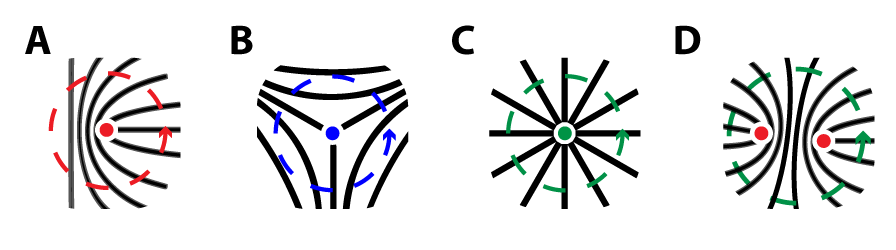
\includegraphics{figures/C2/Ch2-Figs_2DMeas.png}
  \caption{Examples of defect structures and the order parameter space in 2D.
  (A), An $s=+1/2$ defect with the singularity denoted with a red dot.
  The director along the red and purple contours is mapped to $\mathbb{R}\mathbb{P}^1$ in (B).
  (B), A schematic showing $\mathbb{R}\mathbb{P}^1$ (black line) as $\mathbb{S}^1$ (full circle) with antipodal points identified.
  The purple contour in $\mathbb{R}\mathbb{P}^1$ corresponds to the purple contour in real space drawn schematically in (A).
  The purple contour can be continuously deformed to a point in $\mathbb{R}\mathbb{P}^1$.
  (C), A schematic showing $\mathbb{R}\mathbb{P}^1$ (black line) as $\mathbb{S}^1$ (full circle) with antipodal points identified.
  The red contour in $\mathbb{R}\mathbb{P}^1$ corresponds to the purple contour in real space drawn schematically in (A).
  The red contour spans $\mathbb{RP}^1$, and thus has a winding number of +1 in $\mathbb{R}\mathbb{P}^1$ and +1/2 in $\mathbb{S}^1$.
  (D), An $S = -1/2$ defect with the singularity at the blue point.
  In $\mathbb{R}\mathbb{P}^1$, the blue contour would have the same winding as the red contour in (C), but would go the opposite direction.
  (E), An $s = +1$ defect (green dot) encircled by the green contour.
  In $\mathbb{R}\mathbb{P}^1$, the contour would have the same direction as the red contour in (C), but would cover $\mathbb{R}\mathbb{P}^1$ twice and $\mathbb{S}^1$ once.
  (F), Two $s = +1/2$ defects (red dots) placed near to each other such that the green contour encircling both defects sees the same winding in order parameter space as the green contour in (E)
  Thus, far from the defects, we cannot distinguish between structures resulting from a single $s = +1$ defect and two $s = +1/2$ defects, reflecting the additivity of topological charge in 2D.}\label{f:2-2DMeas}
\end{figure}

This approach is not limited to 2D.
In fact, for a general order parameter space $\mathbb{P}$ with dimension $t'$ and a defect with dimension $t$, the codimension $d = t'-t$ defines the order of the homotopy group needed to characterize the defects in $\mathbb{P}$, $\pi_{d}(\mathbb{P})$~\cite{RN236}.
We note that for $d=0$, there are no topological defects in nematic materials as any defect structure with $d=0$ is homotopic to a nonsingular distortion~\cite{RN196}. For example, consider the singular line defect in 2D depicted in Figure~\ref{f:2-Smearing}(A).
Here, the order parameter space is $\mathbb{R}\mathbb{P}^1$, giving $t' = 1$, and the defect is a line with $t = 1$, such that $d = 0$.
This structure can be continuously deformed to remove the singularity, yielding the nonsingular structure in Figure~\ref{f:2-Smearing}(B).
Thus, since a singular line in 2D is homotopic to the undistorted state, it is not topologically stable.
This does not mean that lines in 2D or walls in 3D cannot exist, merely that their existence is determined by energetics such that these structures are usually found only in situations with very strong spatial confinement or in the presence of an external field~\cite{RN33,RN175}.\\
\begin{figure}[h]
  \centering
  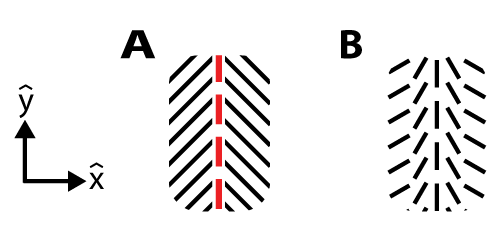
\includegraphics{figures/C2/Ch2-Figs_Smearing.png}
  \caption{Singular line defects are topologically unstable in 2D.
  (A) a singular line defect in 2D, with the singular region denoted in red.
  (B) A nonsingular structure resulting from a continuous deformation of (A).}\label{f:2-Smearing}
\end{figure}

Now, we consider a nematic in 3D.
Immediately, we see that the order parameter space is no longer $\mathbb{R}\mathbb{P}^1$, but instead is $\mathbb{R}\mathbb{P}^2$, the unit 2-sphere $\mathbb{S}^2$ with antipodal points identified, as we now need 2 angles to characterize all the possible orientations of $\mathbf{n}$~\cite{RN196,RN153,RN236}.
Another way to visualize $\mathbb{R}\mathbb{P}^2$ is as a hemisphere where only the base has antipodal points identified.
We first consider line defects with $d=1$ such that we characterize them with $\pi_{1}(\mathbb{R}\mathbb{P}^2)$, the fundamental group of $\mathbb{R}\mathbb{P}^2$.

Again, we consider $\mathbf{n}$ along a closed 1D contour in real space and the associated 1D contour in $\mathbb{R}\mathbb{P}^2$, with the topological charge given by the winding number.
However, we note that in $\mathbb{R}\mathbb{P}^2$, we can only have defects with $s =0,1/2$, as any contour on $\mathbb{R}\mathbb{P}^2$ with an integer value of $s$ can be continuously deformed into a point on $\mathbb{R}\mathbb{P}^2$ since ``you cannot lasso a sphere''~\cite{RN153}.
More explicitly, any contour on  $\mathbb{R}\mathbb{P}^2$ with integer $s$ must start and end at the same point.
Thus it can be ``slid'' to one side of the sphere and deformed to a point on $\mathbb{R}\mathbb{P}^2$, as illustrated schematically in Figure~\ref{f:2-RP2}(A,B).
This means that the only stable contours in $\mathbb{R}\mathbb{P}^2$ are those that start and end at antipodal points [see Figure~\ref{f:2-RP2}(C)], wrapping $\mathbb{R}\mathbb{P}^2$ exactly once.
This also means that contours starting and ending at the same point on $\mathbb{R}\mathbb{P}^2$ can be freely added and subtracted from a contour starting and ending at antipodal points on $\mathbb{R}\mathbb{P}^2$; thus, all contours starting and ending at antipodal points on $\mathbb{R}\mathbb{P}^2$ are homotopic.
Explicitly, this means that contours with $s = -1/2$ are homotopic to contours with $s = 1/2$ such that $\pi_1(\mathbb{R}\mathbb{P}^2)$ has only one nontrivial element, resulting in $s \in \{ 0,1/2\}$~\cite{RN153}.
As with walls in 3D and lines in 2D, this does not mean that $s = +1$ lines in 3D are impossible to create, it only means that they are not topologically stable structures and thus can only be stabilized by energetics.
Similarly, since an $s = -1/2$ line and an $s = +1/2$ line are homotopic, preferentially generating one structure over the other is a matter of tuning the free energy of each structure.
\begin{figure}
  \centering
  
\includegraphics{figures/C2/Ch2-Figs_RP2.png}
  \caption{Contours in $\mathbb{RP}^2$.
  (A--C), Schematics showing $\mathbb{RP}^2$ (blue hemisphere) as $\mathbb{S}^2$ (full sphere) with antipodal points identified.
  A (A) contour that wraps $\mathbb{RP}^2$ twice can be (B) slid off and is homotopic to a point.
  A (C) contour that starts and ends at antipodal points is not homotopic to a point and is the only nontrivial contour in $\mathbb{RP}^2$.}\label{f:2-RP2}
\end{figure}

We lastly consider point defects in 3D characterized by the second homotopy group of $\mathbb{R}\mathbb{P}^2$, $\pi_{2}(\mathbb{R}\mathbb{P}^2)$.
Now, instead of mapping 1D closed contours in real space to $\mathbb{R}\mathbb{P}^1$ and $\mathbb{R}\mathbb{P}^2$ as we did with the fundamental group, we map a topologically spherical surface enclosing the defect to $\mathbb{R}\mathbb{P}^2$~\cite{RN196,RN153,RN236}.
In real space, we restate Eq.~\ref{e:1-HedgehogCharge} and calculate the topological ``hedgehog charge'' of a defect as~\cite{RN153}:
\begin{equation}
  q = \frac{1}{4 \pi} \oint_{\partial V} \textrm{d} \theta \, \textrm{d} \phi \, \mathbf{n} \cdot \left [ \partial_{\theta} \mathbf{n} \times \partial_{\phi} \mathbf{n} \right ],\label{e:2-hedCharge}
\end{equation}
 where $\theta$ and $\phi$ are the polar and azimuthal spherical angles, respectively, and $\partial V$ is the bounding surface of the closed volume $V$ containing the defect.
The volume $V$ must be homotopic to a sphere and thus can have no holes or handles.
From Chapter~\ref{c:1}, we know that this means that the Euler characteristic of $\partial V$ is $\chi = 2$.
Physically, $q$ relates the orientations of $\mathbf{n}$ taken on a topologically spherical surface enclosing the defect to the number of times the orientations cover $\mathbb{S}^2$~\cite{RN153}.
Hedgehog charge is additive such that calculating $q$ for a volume containing only a $+q$ point defect and $-q$ point defect charge will yield $q_{net} = 0$.
Thus, $\pi_{2}(\mathbb{R}\mathbb{P}^2) = (\mathbb{Z}, +)$, the Abelian group consisting of the integers under addition.

It is important to note that there are 2 possible ways to turn a given director field into a vector field; either we take the vectors as $\mathbf{n}$ or as -$\mathbf{n}$.
Since we measure the hedgehog charge by considering how $\mathbf{n}$ on a surface homeomorphic to $\mathbb{S}^2$ covers $\mathbb{RP}^2$, this ambiguity means that any defect in isolation can only be determined up to $|q|$~\cite{RN153}.
Thus, while topological character is determined by homotopy theory, the sign of charge can only be determined relative to a \emph{basepoint} defining the projection from $\mathbb{R}\mathbb{P}^2$ to $\mathbb{S}^2$~\cite{RN153}.
For example, the defect structures drawn schematically in Figure~\ref{f:2-3DMeas}(A,B) cannot be distinguished \emph{a priori} in order parameter space.
However, if we choose a basepoint such that the structure in Figure~\ref{f:2-3DMeas}(A) has $q = +1$, evaluating the structure in Figure~\ref{f:2-3DMeas}(B) under the same basepoint will yield $q = -1$.
We will keep this basepoint for the remainder of the Thesis.
\begin{figure}[h]
  \centering
  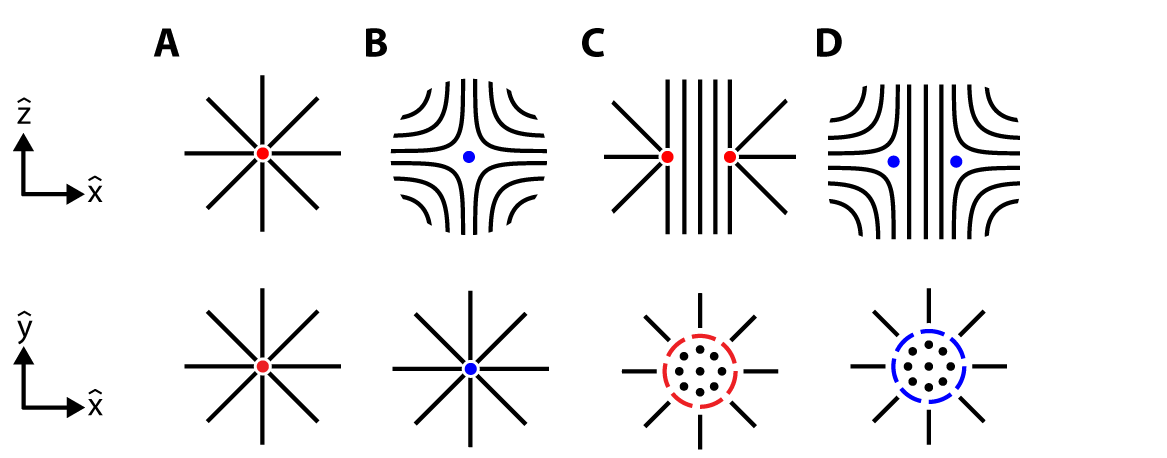
\includegraphics{figures/C2/Ch2-Figs_3DMeas.png}
  \caption{Examples of defect structures in 3D.
  (A-D), Cross sections in the $xz$ and $xy$ planes of defect structures with $|q| = 1$.
  Once we choose a reference point that defines the projection of $\mathbf{n}$ onto the unit sphere, we can distinguish the structures in A,C from the structures in B,D.
  Without loss of generality, we take the convention that the structures in A,C have $q = +1$ such that the structures in B,D have $q = -1$.
  (A,B), schematics of a (A) radial and a (B) hyperbolic hedgehog defect.
  (C,D), schematics of a (C) radial ring and a (D) hyperbolic ring defect.
  Note that the ring defects in (C,D) are formed by an $s = +1/2 $ and an $s = -1/2$ line defect that has closed in on itself.}\label{f:2-3DMeas}
\end{figure}

Similar to how additivity means that a volume enclosing a $+q$ point defect and $-q$ point defect charge will yield $q_{net} = 0$, the point defect structures in Figure~\ref{f:2-3DMeas}(A,B) are not the only structures with $|q| = 1$.
In fact, ring defects, as depicted schematically in Figure~\ref{f:2-3DMeas}(C,D) are homotopic to their respective point defect counterparts in Figure~\ref{f:2-3DMeas}(A,B).
Shrinking the ring radius of the radial ring in Figure~\ref{f:2-3DMeas}(C) yields the radial hedgehog shown in Figure~\ref{f:2-3DMeas}(A) and shrinking the ring radius in the hyperbolic ring in Figure~\ref{f:2-3DMeas}(D) yields a hyperbolic hedgehog like the one shown in Figure~\ref{f:2-3DMeas}(B).
A ring defect can be thought of as a line defect in 3D [see Figure~\ref{f:2-GenDef}] that is bent into a circle.
Hence, if we were to draw a closed 1D contour that passed through the ring and ``linked'' with the ring defect, we would find that radial rings with $q = +1$ are formed with $s = +1/2$ lines and hyperbolic rings with $q = -1$ are formed with $s = -1/2$ lines.

Finally, we briefly want to touch on the use of the term ``charge'' to characterize defects in NLC.\@
The choice of this term is no accident and reflects an analogy with electric charges.
This analogy is born out not only in the additivity of both defect charges and electric charges, but also in their pairwise interactions~\cite{RN33,RN175,RN207}.
Defects in 2D and 3D with like-signed charge repel and defects with opposite-signed charge attract and even annihilate.




\section{Frank-Oseen free energy}
Since the constituent particles, or mesogens, in a nematic material prefer to align along the $\mathbf{n}$, the ideal state for a nematic phase is a homogeneously-aligned state with $\mathbf{n}$ a constant everywhere.
Distortions from this uniform state cost energy.
Since in most experiments the director distortions occur over much larger length scales than the length of the mesogens --- $|\nabla \mathbf{n}| a \ll 1$, where $a$ is the mesogen length --- we can bypass the behavior of individual mesogens and instead use a continuum model for the free energy density that depends on $\mathbf{n}$ only.
Here, we follow the work of F.C. Frank~\cite{RN61} and expand about the undistorted director state in powers of $|\nabla \mathbf{n}|$.
This is a phenomenological approach similar to Hooke's elasticity theory of a solid~\cite{RN175,RN178}; however, instead of focusing on restoring stresses that oppose strains, we look for restoring torques that oppose curvature-strains in the director field.
This is again a reflection that there is no restriction to the center-of-mass positions of the mesogens; the nematic elasticity only opposes deformations in the orientations of the mesogens.

\subsection{A brief derivation}
Let a local coordinate system at a point be defined by $\{x_1, x_2, x_3 \}$ such that we can define $\mathbf{n} = (\mathbf{n} \cdot \hat{e}_i) \hat{e}_i = n_i\hat{e}_i$, where we again sum over repeated indices, and $\hat{e}_i$ is the unit vector associated with $x_i$ and $\{\hat{e}_1, \hat{e}_2, \hat{e}_3 \}$ forms an orthonormal basis.
If we let $\hat{e}_3$ be parallel to $\mathbf{n}$ at the point and consider situations where $x_i \ll 1$, we can locally expand $n_i$ as:
\begin{align}
  n_1 &= \frac{\partial n_1}{\partial x_1}x_1 + \frac{\partial n_1}{\partial x_2}x_2 + \frac{\partial n_1}{\partial x_3}x_3 + \mathcal{O}\big (x^2 \big ) \nonumber \\
      &= a_1 x_1 + a_2 x_2 + a_3 x_3 + \mathcal{O}\big (x^2 \big )\label{e:2-LocalCoordA}  \\
  n_2 &= \frac{\partial n_2}{\partial x_1}x_1 + \frac{\partial n_2}{\partial x_2}x_2 + \frac{\partial n_2}{\partial x_3}x_3 + \mathcal{O}\big (x^2 \big ) \nonumber  \\
      &= a_4 x_1 + a_5 x_2 + a_6 x_3 + \mathcal{O}\big (x^2 \big )\label{e:2-LocalCoordB}  \\
  n_3 &= 1 + \mathcal{O}\big (x^2 \big ). \nonumber
\end{align}
Now expanding about the undistorted state, we can write the free energy density to quadratic order in the first derivatives as:
\begin{equation}
  f(\mathbf{n}) = K_i a_i + K_{ij} a_i a_j,\label{e:2-FrankGeneralExpansion}
\end{equation}
where $i,j = \{ 1,2 \dots, 6 \}$, giving us 42 possible terms.
However, any free energy must respect the symmetry of the nematic phase and be invariant under exchange of $i$ and $j$, invariant under inversion of $\mathbf{n} \rightarrow -\mathbf{n}$, invariant under arbitrary rotations about $\mathbf{n}$, and invariant with respect to the handedness of the coordinate system~\cite{RN61}.
Under these conditions, all of the 6 $K_i$ terms vanish and of the 36 terms in $K_{ij}$, 26 vanish and only 4 are independent, giving the coefficient matrix:
\begin{equation}
  K_{ij} =
  \begin{pmatrix}
    K_{11} & 0 & 0 & 0 & (K_{11}-K_{22}-K_{24}) & 0 \\
    0 & K_{22} & 0 & K_{24} & 0 & 0 \\
    0 & 0 & K_{33} & 0 & 0 & 0 \\
    0 & K_{24} & 0 & K_{22} & 0 & 0 \\
    (K_{11}-K_{22}-K_{24}) & 0 & 0 & 0 & K_{11} & 0 \\
    0 & 0 & 0 & 0 & 0 & K_{33} \\
  \end{pmatrix}.\label{e:2-Kijreduced}
\end{equation}
Substituting Eq.~\ref{e:2-Kijreduced} into Eq.~\ref{e:2-FrankGeneralExpansion} and collecting terms, we are left with the expression:
\begin{align}
  f(\mathbf{n}) = \frac{1}{2}K_{11} (a_1 + a_5)^2 + \frac{1}{2}&K_{22} (a_2 - a_4)^2 + \frac{1}{2}K_{33} (a_3^2 + a_6^2) \nonumber \\
    &- (K_{22} + K_{24}) (a_1 a_5 - a_2 a_4).\label{e:2-FrankLocalExpansion}
\end{align}
If we return to the source of the $a_i$ coefficients in Eqs.~\ref{e:2-LocalCoordA}, \ref{e:2-LocalCoordB}, we can uncover the physical significance of the distortions:
\begin{align}
  s_1 = a_1 = \frac{\partial n_1}{\partial x_1} \quad & \quad s_2 = a_5 = \frac{\partial n_2}{\partial x_2}\label{e:2-PhysicalDistortionsA} \\
  t_1 = - a_4 = -\frac{\partial n_2}{\partial x_1} \quad & \quad t_2 = a_2 = \frac{\partial n_1}{\partial x_2}\label{e:2-PhysicalDistortionsB} \\
  b_1 =  a_3 = \frac{\partial n_1}{\partial x_3} \quad & \quad b_2 = a_6 = \frac{\partial n_2}{\partial x_3},\label{e:2-PhysicalDistortionsC}
\end{align}
where we have renamed the coefficients to reflect their associated distortion, with $s_1$ and $s_2$ signifying a ``splay'' distortion, $t_1$ and $t_2$ signifying a ``twist'' distortion, and $b_1$ and $b_2$ signifying a ``bend'' distortion.
These distortions in the local frame are easily visualized, as seen in Figure~\ref{f:2-FrankDist}(A--C), respectively.
Now if we use Eqs.~\ref{e:2-PhysicalDistortionsA}--\ref{e:2-PhysicalDistortionsC} to re-write Eq.~\ref{e:2-FrankLocalExpansion}, we have:
\begin{align}
  f(\mathbf{n}) = \frac{1}{2}K_{11} (s_1 + s_2)^2 + \frac{1}{2}&K_{22} (t_1 + t_2)^2 + \frac{1}{2}K_{33} (b_1^2 + b_2^2) \nonumber \\
    & - (K_{22} + K_{24}) (s_1 s_2 + t_1 t_2).\label{e:2-FrankPhysicalExpansion}
\end{align}

\begin{figure}
  \centering
  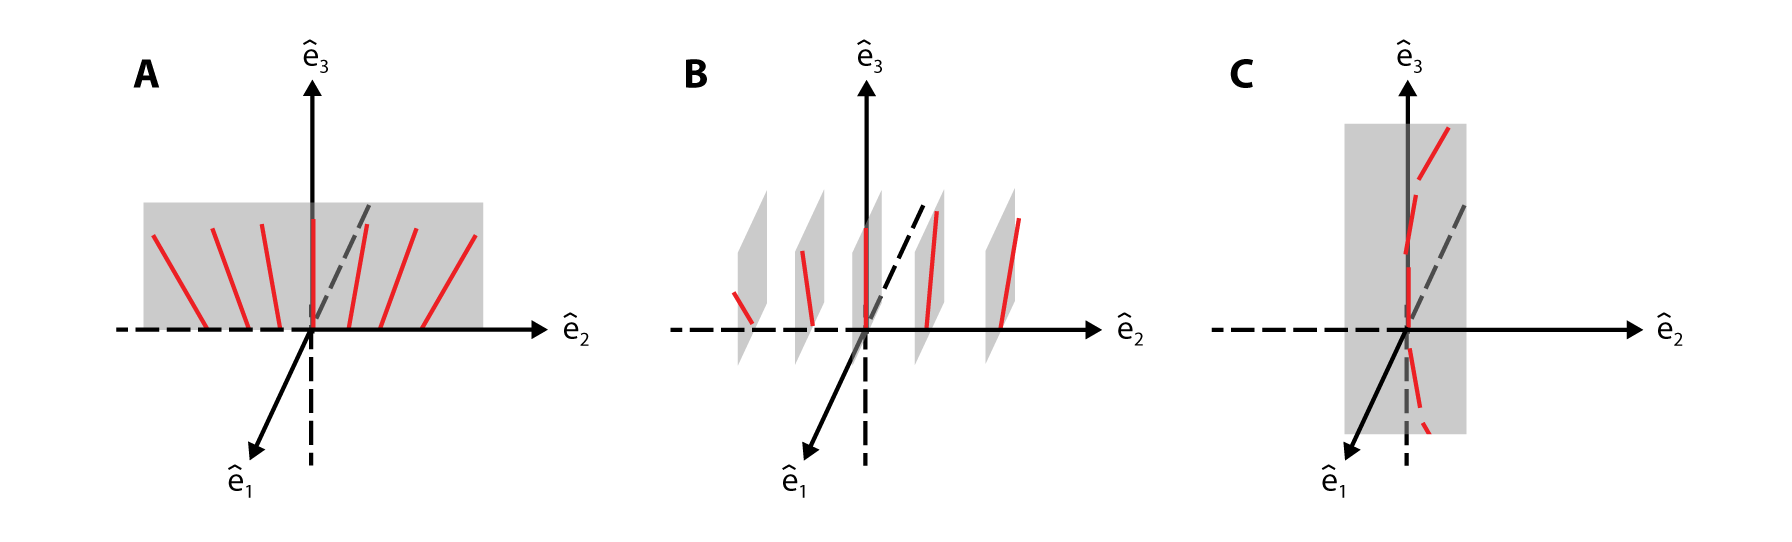
\includegraphics{figures/C2/Ch2-Figs_FrankDist.png}
  \caption{Nematic distortions in the local frame. (A), A schematic showing a splay distortion corresponding to a nonzero $s_2$.
  (B), A schematic showing a twist distortion corresponding to a nonzero $t_2$.
  (C), A schematic showing a bend distortion corresponding to a nonzero $b_2$.}\label{f:2-FrankDist}
\end{figure}
Hence, we see that each term in the free energy density comes from a different distortion, such that the elastic constants $K_{ij}$ hold the relative importance of each distortion for a given material.
For example, consider a NLC with $K_{11} \gg K_{33} = K_{22} = K_{24}$; under confinement or strain, this material will prefer to bend and twist instead of splay.
The elastic constants are named after their associated distortion, with $K_{11}$ known as the splay elastic constant, $K_{22}$ the twist elastic constant, $K_{33}$ the bend elastic constant, and $K_{24}$ the saddle-splay elastic constant.
Note that the saddle-splay distortion is unique as it is associated with both the twist elastic constant and the saddle-splay elastic constant.

The ability to associate individual distortions with their elastic constant gives the Frank-Oseen free energy incredible intuitive power; it is easy to visualize each distortion's contribution to the director field.
Finally, we can recast the distortions in Eq.~\ref{e:2-FrankLocalExpansion} in terms of standard vector calculus operations, arriving at the well-known expression for the Frank-Oseen Free Energy~\cite{RN61}:
\begin{align}
  f(\mathbf{n}) = \frac{1}{2}K_{11} (\nabla \cdot \mathbf{n})^2 + \frac{1}{2}&K_{22} (\mathbf{n} \cdot \nabla \times \mathbf{n})^2 + \frac{1}{2}K_{33} (\mathbf{n} \times \nabla \times \mathbf{n})^2 \nonumber \\
    & - \frac{1}{2}(K_{22} + K_{24}) \nabla \cdot (\mathbf{n}\nabla \cdot \mathbf{n} + \mathbf{n} \times \nabla \times \mathbf{n}).\label{e:2-FrankFinalExpansion}
\end{align}

Note that while Frank pioneered the phenomenological approach for a liquid crystalline free energy, his was not the first attempt to construct a free energy for liquid crystals.
Oseen arrived at a similar expression to Eq.~\ref{e:2-FrankFinalExpansion} before Frank, but he approached the problem from a microscopic approach under the assumption that the free energy could be calculated considering interactions between all possible pairs of molecules~\cite{RN205}.
While Oseen's final expression for a nematic misses some of the terms in Eq.~\ref{e:2-FrankFinalExpansion}, it is close enough that Eq.~\ref{e:2-FrankFinalExpansion} carries the names of both Frank and Oseen.


\subsection{Nehring, Saupe, and second derivatives}
We arrived at Eq.~\ref{e:2-FrankFinalExpansion} by expanding about the undistorted state to quadratic order in powers of the 1$^\textup{\rm st}$ derivatives of $\mathbf{n}$.
Due to the symmetry of the nematic, all of the terms linear in $|\nabla \mathbf{n}|$ vanished, making the quadratic terms the lowest order surviving terms in the expansion.
However, as Nehring and Saupe pointed out, a full expansion to the lowest order should also include 2$^\textup{\rm nd}$ derivatives of $\mathbf{n}$ as they can contribute to the Frank-Oseen free energy at order $\mathcal{O}(x^2)$ as well~\cite{RN60}.
In fact, Oseen's original free energy expression also included terms depending on 2$^\textup{\rm nd}$ derivatives of $\mathbf{n}$ that Frank neglected~\cite{RN205}.
Thus, Eq.~\ref{e:2-FrankGeneralExpansion} becomes:
\begin{equation}
  f(\mathbf{n}) = K_i a_i + K_{ij} a_i a_j + K'_{ij} a_{i,j},\label{e:2-NSGeneralExpansion}
\end{equation}
where $a_{i,j}$ represents $\dfrac{\partial a_i}{\partial x_j}$, giving us 18 terms in the $K'_{ij}$ coefficient matrix.
Again using the symmetries of a nematic, collecting terms, and rewriting the expression in terms of vector calculus manipulations, we arrive at a new expression for the free energy:
\begin{align}
  f(\mathbf{n}) = \frac{1}{2}&(K_{11} - 2K'_{13}) (\nabla \cdot \mathbf{n})^2 + \frac{1}{2}K_{22} (\mathbf{n} \cdot \nabla \times \mathbf{n})^2 + \frac{1}{2}(K_{33} + 2K'_{13}) (\mathbf{n} \times \nabla \times \mathbf{n})^2 \nonumber \\
    & - \frac{1}{2}(K_{22} + K_{24}) \nabla \cdot (\mathbf{n}\nabla \cdot \mathbf{n} + \mathbf{n} \times \nabla \times \mathbf{n})
      + K'_{13} \nabla \cdot (\mathbf{n} \nabla \cdot \mathbf{n}),\label{e:2-NSFinalExpansion}
\end{align}
where we see that the elastic constants associated with splay and bend are renormalized by $K'_{13}$, and that a new term called ``splay-bend'' associated with the distortion $\nabla \cdot (\mathbf{n} \nabla \cdot \mathbf{n})$ has appeared~\cite{RN60}. \\

Since Eqs~\ref{e:2-FrankFinalExpansion} and~\ref{e:2-NSFinalExpansion} are phenomenological expressions, renormalizing the splay and bend elastic constants doesn't affect underlying physics.
This leaves the addition of the splay-bend term as the most significant effect of considering 2$^\textup{\rm nd}$ order derivatives of $\mathbf{n}$.
The splay-bend term itself is subject to controversy as its inclusion to the free energy makes the free energy unbounded from below~\cite{RN214,RN215,RN216}.
We follow Ref.~\cite{RN219} and illustrate this with a simple example of a NLC confined between two parallel plates.
Let one plate be at $z = 0$ and the other at $z=d$, and let the director vary only in the $xz$-plane.
We can then write our director in terms of the angle $\phi$ in the $xz$-plane measured off of the $x$-axis.
Let the director field have the form $\phi_n(z) = \phi_d + \beta ((z/d)^n-1)$, such that $\phi(0) = \phi_d - \beta$ and $\phi(d) = \phi_d$, with $\phi_d$ and $\beta$ fixed angles that give the boundary conditions.
In this case, $n$ is a positive integer that governs how the director varies between the two plates.
This geometry is known as the splay-bend geometry.
For simplicity, we take $K_{11} = K_{33} = K$, and assume $n$ is large, allowing us to approximate the free-energy as,
\begin{align}
  F &\approx \frac{1}{4}\frac{K \beta^2}{d^2} \left ( 1 + \frac{2 K_{13} \sin(2 \phi_d)}{K \beta}  \right) n.\label{e:2-UnboundedFromBelow}
\end{align}
If we require $|\beta|K < 2| K_{13} \sin(2 \phi_d)| $ and $K_{13} \sin(2 \phi_d)/\beta < 0$, then the \\ $1 + 2 K_{13} \sin(2 \phi_d)/(K \beta) $ term in Eq.~\ref{e:2-UnboundedFromBelow} is negative, and
\begin{align}
  \lim_{n\to\infty} &F = -\infty, \\
  \lim_{n\to\infty} &\phi_n(z) =
  \begin{cases}
    \phi_d - \beta \quad \textrm{if }  0 \leq z  < d \\
    \phi_d \quad \textrm{if } z = d.
  \end{cases}
\end{align}
Here, we see that that our director field has a free energy that diverges to $- \infty$, leading to a discontinuity in our director field.
The discontinuity is called the Oldano-Barbero discontinuity.
Recall that we initially derived the Frank-Oseen free energy assuming small deformations --- however, we have just shown a situation where the Frank-Oseen free energy diverges and leads to a discontinuity in the director field.
This situation is called the Oldano-Barbero paradox~\cite{RN216,RN220,RN219,RN221}.

The easiest way to solve the paradox is to set $K'_{13} = 0$.
It is worth noting that there has been a concerted effort to solve the paradox without setting $K'_{13} = 0$~\cite{RN220,RN221,RN55,RN222}.
However, careful experiments in the splay-bend geometry have found $K'_{13} = 0$ within experimental error, and the experimenters never observe a discontinuity in the director field~\cite{RN312}.
Consequently, the most common approach is to neglect the splay-bend term altogether~\cite{RN55,RN222}.


\subsection{Insights from microscopic calculations}
There has been significant theoretical effort, starting with the pioneering work of Oseen, to relate the microscopic interactions between the nematic mesogens to the macroscopic, measurable $K_{ij}$ of the nematic phase~\cite{RN56,RN55,RN205,RN217,RN225,RN224,RN218,RN222}.
While an in-depth discussion of the various methods and results is beyond the scope of this document, it is worthwhile to examine the general process and consider the implications for the $K_{ij}$ in the phenomenological expressions derived earlier.
At the most basic level, the total interaction energy for a system is the sum over the pairwise interaction energy for all pairs of mesogens in the system.

However, an energy constructed upon the physical mesogens themselves requires us to know the position and orientation of each individual mesogen.
Thus, it is common to consider instead the particle density as a function of orientation and position and integrate over all possible pairs of points in the volume~\cite{RN222}.
This is a density functional theoretic approach~\cite{RN223} and thus yields an energy similar to the general expression~\cite{RN56,RN55}:
\begin{equation}
  F = \int \textrm{d}\mathbf{R} \textrm{d}\mathbf{R}' \, G(\mathbf{R},\mathbf{R}'),
\end{equation}
where $\mathbf{R}$ and $\mathbf{R}'$ are positions, and $G(\mathbf{R},\mathbf{R}')$ is an interaction energy density satisfying $G(\mathbf{R},\mathbf{R}') = 0$ for $|\mathbf{R}-\mathbf{R}'| \gg 0$, reflecting the finite interaction range between the mesogens.
However, we are looking for a free energy and not just the interaction energy of the system.
Thus, it is common to calculate the energy for a homogeneous state and then expand about the homogeneous state to get an expression for a distortion free energy, $\delta F$; this is similar to how we derived the Frank-Oseen free energy earlier.
Since we are looking to derive an expression for the free energy as a functional of director field, we must satisfy
\begin{equation}
  \delta F = \int \textrm{d}\mathbf{R} \textrm{d}\mathbf{R}' \, G(\mathbf{R},\mathbf{R}')
  = \int \textrm{d} \mathbf{r} \, f(\mathbf{r}),\label{e:2-NonlocalLocal}
\end{equation}
where $f(\mathbf{r})$ is a function of position, $\mathbf{r}$.
Note that there is not a unique relation between $f(\mathbf{r})$ and $G(\mathbf{R},\mathbf{R}')$; more specifically, $f$ will be determined by how we choose $r$.
For example, if $\mathbf{r} = \mathbf{R}$, then $f(\mathbf{r}) = \int \textrm{d}\mathbf{R}' \, G(\mathbf{r},\mathbf{R}')$.
However, if $\mathbf{r} = (\mathbf{R} + \mathbf{R}')/2$, then $f(\mathbf{r}) = \int \textrm{d}\mathbf{R}' \, G(2\mathbf{r} - \mathbf{R}',\mathbf{R}')$.
Since there are an infinite number of possibilities to choose $\mathbf{r}$ and thus determine $f$, any elastic constants in $f(\mathbf{r})$ cannot depend on how we choose $\mathbf{r}$~\cite{RN55}.
% In addition, the microscopic calculations are performed with a density function that is dependent on position and orientation, $\rho(\mathbf{r},\mathbf{\omega})$, where $\mathbf{\omega}$ specifies an orientation; however, the phenomenological free energy expressions are only a function of the director field.
% Thus, we must also satisfy:
% \begin{equation}
%   F[\mathbf{n}(\mathbf{r})] = \int \textrm{d} \mathbf{r} \, f(\mathbf{n}(\mathbf{r})) = \int \textrm{d} \mathbf{r}\,\textrm{d} \omega \, f \big ( \rho(\mathbf{r},\mathbf{\omega}) \big).\label{e:2-LessInfo}
% \end{equation}
% Since the director contains less information than the complete density function, in general there is not a unique way to determine $\mathbf{n}(\mathbf{r})$ from $\rho(\mathbf{r},\mathbf{\omega})$~\cite{RN55}.
% For a distortion of wavelength $\xi$ and amplitude $\epsilon$, we can only uniquely determine $\mathbf{n}(\mathbf{r})$ if we restrict ourselves to the lowest energy distortions in the long-wavelength $(\xi \rightarrow \infty)$ and small amplitude $(\epsilon \ll 1)$ regime.
% These modes come from the Nambu-Goldstone theorem, which requires that any broken continuous symmetry results in a soft mode, i.e.\ a mode whose distortion cost vanishes as $\xi^{-2}$ and whose susceptibility diverges in the limit $\xi \rightarrow \infty$~\cite{RN175,RN226,RN227,RN228}.
% These soft modes are the weakest modes possible and thus will define the leading order in the free energy, making the free energy a unique functional of $\mathbf{n}$~\cite{RN55}. \\

Given this condition, microscopic calculations show that $K_{11}$, $K_{22}$, $K_{33}$, and $K_{24}$ are real physical material properties~\cite{RN55,RN56,RN225,RN224,RN217,RN222}.
However, $K'_{13}$ depends on the choice of $\mathbf{r}$, and therefore cannot be a real material parameter.
Physically, we can think about this result in terms of how the free energy scales in terms of the amplitude, $\epsilon$, and wavelength, $\zeta$, of an arbitrary distortion in a NLC.
Since $K_{11}$, $K_{22}$, $K_{33}$, and $K_{24}$ are all composed of only $1^{\rm st}$ derivatives, their contribution to the free energy $\sim (\epsilon/\zeta)^2$.
However, $K_{13}'$ is a $2^{\rm nd}$ derivative with a contribution to the free energy $\sim \epsilon/(\zeta^2)$.
This linear dependence on the amplitude in the $K_{13}'$ distortion makes the homogeneous director state unstable to long wavelength ($\zeta \rightarrow \infty$) distortions, where the energetic cost of a distortion vanishes~\cite{RN55}.
Consequently, $K'_{13} = 0$ and the common approach of neglecting splay-bend is valid.~\cite{RN55,RN225}.
With $K_{13}'=0$, we see that Eq.~\ref{e:2-NSFinalExpansion} reduces to the expression for the Frank-Oseen free energy in Eq.~\ref{e:2-FrankFinalExpansion}.
% The conclusion that $K'_{13} = 0$ also holds when calculations are done close to a boundary provided the $\mathbf{n} = -\mathbf{n}$ inversion symmetry is maintained~\cite{RN56}.
% Since inversion symmetry is assumed in deriving the phenomenological expressions in Eqs.~\ref{e:2-NSFinalExpansion} and~\ref{e:2-FrankFinalExpansion}, situations that violate inversion symmetry create far more issues than simply the inclusion of a $K_{13}'$ term.
% Note that while there have been microscopic calculations that predict a nontrivial $K'_{13}$, these calculations~\cite{RN224,RN217,RN222} have specified a $(\mathbf{R},\mathbf{R}') \rightarrow \mathbf{r}$ mapping, rendering their $K'_{13}$ values invalid.

Microscopic calculations also show that close to a boundary, $K_{ij}$ in general deviate from their bulk values and become position-dependent.
This is because the mesogens are now interacting with the material outside of the nematic volume~\cite{RN56,RN57,RN55}.
However, this interaction is limited by the range of the intermolecular potential, such that the position dependence of the $K_{ij}$ vanishes over a small boundary layer --- beyond this layer the $K_{ij}$ return to their bulk values, which depend only on the specific nematic material.

In summary, microscopic calculations show that the free energy of a NLC is composed of terms quadratic in $|\nabla \mathbf{n}|$.
Even though terms linear in $|\nabla ^2 \mathbf{n}|$ could in principle contribute to the free energy to the same order as terms quadratic in the 1$^\textup{\rm st}$ derivatives, microscopic calculations show that the coefficients associated with 2$^\textup{\rm nd}$-derivative distortions vanish, thus removing the problems that the 2$^\textup{\rm nd}$-derivative distortions bring.
% In addition, since the free energy is constructed using a positive-definite pairwise potential, all the elastic constants in the phenomenological free energy expressions must be greater than or equal to 0.


\subsection{Saddle-splay and curvature-coupling}
If we take a look at the terms in the Frank-Oseen free energy in Eq.~\ref{e:2-FrankFinalExpansion}, we can see a difference between the saddle-splay term and the splay, twist, and bend terms.
Notice that since all the $K_{ij} \geq 0$, the energetic cost of splay, bend, and twist distortions are positive semi-definite.
In contrast, the saddle-splay distortion can be either positive or negative.
In addition, the saddle-splay distortion is the divergence of a vector, giving us the option of re-writing the distortion in terms of a surface integral using the divergence theorem~\cite{RN230}:
\begin{align}
  F_{24}[\mathbf{n}] &= - \frac{1}{2}\int_{V} \textup{d}^3  \mathbf{r} \bigg \{ (K_{22} + K_{24})  \nabla \cdot (\mathbf{n}\nabla \cdot \mathbf{n} + \mathbf{n} \times \nabla \times \mathbf{n}) \bigg \}\label{e:2-F24GaussA}  \\ &=
  - \frac{1}{2}(K_{22} + K_{24}) \oint_{\partial V} \textup{d}^2  \mathbf{r} \bigg \{   \mathbf{k} \cdot (\mathbf{n}\nabla \cdot \mathbf{n} + \mathbf{n} \times \nabla \times \mathbf{n}) \bigg \},\label{e:2-F24GaussB}
\end{align}
where $V$ is a volume, $\partial V$ is a piecewise-smooth manifold bounding $V$, and $\mathbf{k}$ is the unit surface normal.

Note that the $\mathbf{n}$ needs to be continuous and differentiable everywhere on $\partial V$, meaning that the manifold needs to be defect-free.
However, since $\partial V$ only needs to be piecewise continuous, we can always draw the manifold to exclude any defects.
Therefore, the divergence theorem can always be applied, implying that any nontrivial saddle-splay distortion in $V$ must affect $\mathbf{n}$ on $\partial V$.
In contrast, nontrivial splay, bend, and twist distortions can exist purely in the bulk, such that $\mathbf{n}$ is affected in $V$ but not on $\partial V$.
In fact, the ability to generate pure bulk distortions for splay, twist, and bend allow for easy measurements of $K_{ij}$ via the Freederickz transition, for example~\cite{RN212,RN213,RN33,RN188,RN182,RN183}.
In these measurements, the bulk volume is always large enough such that any contribution from the position-dependence of $K_{ij}$ near the boundaries is negligible.

Due to the connection between the bulk saddle-splay distortion and the director orientation on a bounding manifold, the saddle-splay distortion term is often referred to as a surface-like term and sometimes even referred to as an effective anchoring term~\cite{RN206,RN33,RN194,RN58,RN57,RN151}.
Since any measurement of $K_{24}$ requires $\mathbf{n}$ to change at an interface, there is concern that the position-dependence of $K_{ij}$ near an interface leads to the inability to measure the bulk value of $K_{24}$ without contamination from the interface.
However, we emphasize that while it is tempting to treat $F_{24}$ as a surface term where the energy cost is calculated using the value of $K_{ij}$ at the interface like,
\begin{equation}
  F_{24}[\mathbf{n}] = - \frac{1}{2}(K_{22}(\mathbf{r}) + K_{24}(\mathbf{r}))_{\mathbf{r} \rightarrow \partial V} \oint_{\partial V} \textup{d}^2  \mathbf{r} \bigg \{   \mathbf{k} \cdot (\mathbf{n}\nabla \cdot \mathbf{n} + \mathbf{n} \times \nabla \times \mathbf{n}) \bigg \},
\end{equation}
this is incorrect.
The divergence theorem cannot be used if $K_{ij}$ is position-dependent since the integrand in Eq.~\ref{e:2-F24GaussA} is no longer the divergence of a vector.
In fact, measuring $K_{24}$ is in principle no different than measuring any of the $K_{ii}$ --- provided the volume of the bulk is much larger than the boundary layer, the influence of the position-dependence of $K_{ij}$ is negligible.

To demonstrate this, we return to Eq.~\ref{e:2-F24GaussA} and insert the position-dependence:
\begin{equation}
  F_{24} = -\frac{1}{2}\int_{V}\textup{d}^3\mathbf{r} \left \{ (K_{22} (\mathbf{r}) + K_{24}(\mathbf{r})) \nabla \cdot (\mathbf{n} \nabla \cdot \mathbf{n} + \mathbf{n} \times \nabla \times \mathbf{n}) \right \}.\label{e:2-F24GaussPosition}
\end{equation}
Integrating Eq.~\ref{e:2-F24GaussPosition} by parts with $\mathbf{A}(\mathbf{r}) = \mathbf{n} \nabla \cdot \mathbf{n} + \mathbf{n} \times \nabla \times \mathbf{n}$, \newline $K_*(\mathbf{r}) = -(K_{22} (\mathbf{r}) + K_{24}(\mathbf{r})/2)$, and $\bm{\alpha}$ describing the boundary yields:
\begin{align}
  \int_{V}\textup{d}^3\mathbf{r} \left \{ K_{*} (\mathbf{r}) \nabla \cdot \mathbf{A} \right \} &=
  \oint_{\partial V}\textup{d}^2 \mathbf{r} \left \{ \mathbf{k} \cdot (K_{*} (\bm{\alpha}) \mathbf{A}(\bm{\alpha}) \right \} -  \int_{V} \textup{d}^3\mathbf{r} \left \{ \mathbf{A} \cdot \nabla K_{*} (\mathbf{r}) \right \}  \\ &=
  K_*(\bm{\alpha}) \oint_{\partial V} \textup{d}^2\mathbf{r} \left \{ \mathbf{k} \cdot \mathbf{A}(\bm{\alpha})\right \} - \int_{V} \textup{d}^3\mathbf{r} \left \{ \mathbf{A} \cdot \nabla K_{*} (\mathbf{r}) \right \}, \label{e:2-pos_stokes1}
\end{align}
where we have chosen $\mathbf{k}$ as the outward-pointing unit normal and we have pulled $K_*(\partial V)$ out of the integral as $K_*$ only depends on the distance from the boundary~\cite{RN55}.
Now, we separate $K_*(\mathbf{r}) = K_* + K_*^s(\mathbf{r})$ into the bulk material constant $K_*$ and the position-dependent contribution $K_*^s(\mathbf{r})$, where $K_*^s(\mathbf{r})$ decays across a boundary layer of thickness $d_l$.
Substituting this into Eq.~\ref{e:2-pos_stokes1}, we are left with:
\begin{align}
  \int_{V}\textup{d}^3\mathbf{r} \left \{ K_{*} (\mathbf{r}) \nabla \cdot \mathbf{A} \right \} &=
  (K_*+K_*^s(\bm{\alpha})) \oint_{\partial V} \textup{d}^2\mathbf{r} \left \{ \mathbf{k} \cdot \mathbf{A}(\bm{\alpha})\right \} \nonumber \\&
  \quad \quad - \int_{V} \textup{d}^3\mathbf{r} \left \{ \mathbf{A} \cdot \nabla K_{*}^s (\mathbf{r}) \right \}. \label{e:2-pos_stokes2}
\end{align}
If we now expand $\mathbf{A}(\mathbf{r})$ and $\nabla K_*^s(\mathbf{r})$ over the boundary layer with $\mathbf{r} = \bm{\alpha} - \zeta \mathbf{k}$, where $\zeta$ is the distance from the boundary, we have:
\begin{align}
  \mathbf{A}(\bm{\alpha} - \zeta \mathbf{k}) &\approx \mathbf{A}(\bm{\alpha}) - \zeta (\mathbf{k} \cdot \nabla \mathbf{A}(\bm{\alpha}))_{\zeta = 0} \label{e:2-expandA} \\
  \nabla K_*^s(\bm{\alpha} - \zeta \mathbf{k}) &\approx \mathbf{k} (\mathbf{k} \cdot \nabla K_*^s(\bm{\alpha} - \zeta \mathbf{k}))_{\zeta = 0} - \zeta\, \mathbf{k}(\mathbf{k} \cdot \nabla (\mathbf{k} \cdot \nabla K_*^s(\bm{\alpha} - \zeta \mathbf{k})))_{\zeta = 0}
\end{align}
As $K_*^s(\mathbf{r})$ decays across a boundary layer of thickness $d_l$, we can approximate the leading order term in $\nabla K_*^s(\bm{\alpha} - \zeta \mathbf{k})$ as:
\begin{equation}
  \mathbf{k} (\mathbf{k} \cdot \nabla K_*^s(\bm{\alpha}))_{\zeta = 0} =
  \begin{cases}
    \mathbf{k}\frac{K_*^s(\bm{\alpha})}{d_l} & 0 \leq \zeta \leq d_l \\
    0 & \textup{otherwise}
  \end{cases}
\end{equation}
Thus, to leading order we can write the 2$^\textrm{\rm nd}$ term in Eq.~\ref{e:2-pos_stokes2} as
\begin{align}
  \int_{V} \textup{d}^3\mathbf{r} \left \{ \mathbf{A} \cdot \nabla K_{*}^s (\mathbf{r}) \right \} & \approx
  \int_{V} \textup{d}^3\mathbf{r} \left \{\mathbf{A}(\bm{\alpha}) \cdot \mathbf{k}(\mathbf{k} \cdot \nabla K_*^s(\bm{\alpha}))  + \mathcal{O}(\zeta) \right \} \\ & \approx
  \mathbf{k} \cdot \nabla K_*^s(\bm{\alpha}) \int_{V} \textup{d}^3\mathbf{r}\left \{\mathbf{A}(\bm{\alpha}) \cdot \mathbf{k} + \mathcal{O}(\zeta) \right \} \\ & \approx
  \frac{K_*^s(\bm{\alpha})}{d_l} \oint_{\partial V} \textup{d}^2\mathbf{r}\left \{d_l\,\mathbf{A}(\bm{\alpha}) \cdot \mathbf{k} \right \} \\ & \approx
  K_*^s(\bm{\alpha}) \oint_{\partial V} \textup{d}^2\mathbf{r}\left \{ \mathbf{k}  \cdot \mathbf{A}(\bm{\alpha}) \right \} + \mathcal{O}(d_l^2).
\end{align}
Substituting back into Eq.~\ref{e:2-pos_stokes2}, we have:
\begin{equation}
  \int_{V}\textup{d}^3\mathbf{r} \left \{ K_{*} (\mathbf{r}) \nabla \cdot \mathbf{A} \right \} \approx
  K_* \oint_{\partial V} \textup{d}^2\mathbf{r} \left \{ \mathbf{k} \cdot \mathbf{A}(\bm{\alpha})\right \},\label{e:2-positionF24}
\end{equation}
giving us the saddle-splay contribution to the free energy,
\begin{equation}
  F_{24} \approx -\frac{1}{2}(K_{22} + K_{24})
  \oint_{\partial V}\textup{d}^2 \mathbf{r} \left \{\mathbf{k} \cdot (\mathbf{n} \nabla \cdot \mathbf{n} + \mathbf{n} \times \nabla \times \mathbf{n}) \right \} + \mathcal{O}(d_l^2). \label{e:2-positionF24_surf}
\end{equation}
Thus, even though the saddle-splay distortion must be measured in the presence of an interface, where $K_{ij}$ are position-dependent, the free energy of the saddle-splay distortion is primarily driven by the bulk value of $K_{24}$ and $K_{22}$ with corrections on the order of the square of the boundary layer thickness.

The saddle-splay distortion can also serve to couple the director to the curvature of the interface.
Consider a nematic constrained to lie in the plane of the interface.
Then, ignoring the corrections in Eq.~\ref{e:2-positionF24_surf} for simplicity, we can write the free energy of the saddle-splay distortion as:
\begin{equation}
  F_{24} = -\frac{1}{2}(K_{22} + K_{24})
  \oint_{\partial V}\textup{d}^2 \mathbf{r} \left \{\mathbf{k} \cdot ( \mathbf{n} \times \nabla \times \mathbf{n}) \right \},\label{e:2-K24PlanDegen}
\end{equation}
since $\mathbf{n} \cdot \mathbf{k} = 0$. Now rearranging the integrand, we can take advantage of the fact that $\mathbf{n} \cdot \mathbf{n}=1$ and write:
\begin{align}
  \mathbf{k} \cdot ( \mathbf{n} \times \nabla \times \mathbf{n}) &=\mathbf{k} \cdot \mathbf{n} \cdot (\nabla \mathbf{n}) -\mathbf{k} \cdot (\mathbf{n} \cdot \nabla)\mathbf{n}  \\
   &= -\mathbf{k} \cdot (\mathbf{n} \cdot \nabla)\mathbf{n}.\label{e:2-K24rearrange1}
\end{align}

Again taking advantage of the fact that $\mathbf{k} \cdot \mathbf{n} = 0$, we can re-write $\mathbf{n}$ in terms of an orthonormal basis defined on the surface like $\mathbf{n} = (\hat{e}_i \cdot \mathbf{n})\hat{e}_i$, where now $i = 1,2$.
Note that our director is now in 2D as we have restricted $\mathbf{n}$ to be on the surface.
Re-writing the right-hand side (RHS) of Eq.~\ref{e:2-K24rearrange1}, we have:
\begin{align}
  -\mathbf{k} \cdot (\mathbf{n} \cdot \nabla)\mathbf{n}
  &= \mathbf{n} \cdot (\mathbf{n} \cdot \nabla)\mathbf{k} - (\mathbf{n} \cdot \nabla)(\mathbf{k} \cdot \mathbf{n}) \\
  &= \mathbf{n} \cdot (\mathbf{n} \cdot \nabla)\mathbf{k} \\
  &= n_i \hat{e}_i \cdot (n_j \hat{e}_j \cdot \nabla) \mathbf{k} \\
  &=- n_i n_j \big ( - \hat{e}_i \cdot ( \hat{e}_j \cdot \nabla) \mathbf{k} \big ) \\
  &= - n_i L_{ij} n_j \\
  &= -\mathbf{n} \cdot \mathbf{L} \cdot \mathbf{n},\label{e:2-K24rearrange2}
\end{align}
where $\mathbf{L}$ is the Weingarten Matrix whose components are~\cite{RN23,RN35}:
\begin{equation}
  L_{ij} = - \hat{e}_i \cdot (\hat{e}_j \cdot \nabla) \mathbf{k}\label{e:2-WeingartenMatrix}
\end{equation}

The Weingarten Matrix describes how a curved surface changes in space, and its invariants give the mean and Gaussian curvature of the surface: $H = \textrm{tr}\{\mathbf{L}\}/2$ and $K = \textrm{det} \{ \mathbf{L} \}$, respectively.
As $K = \kappa_1 \kappa_2$, we see that finding $\kappa_1$ and $\kappa_2$, the principal curvatures, becomes an eigenvalue problem; the eigenvectors of $\mathbf{L}$ give the principal curvature directions, and the associated eigenvalues are the principal curvatures themselves.
Now, choosing $\hat{e}_1$ and $\hat{e}_2$ as the principal curvature directions, then we can write the saddle-splay free energy in terms of $\kappa_1$ and $\kappa_2$ as~\cite{RN59}:
\begin{equation}
  F_{24} = \frac{1}{2}(K_{22} + K_{24})
  \oint_{\partial V}\textup{d}^2 \mathbf{r} \left \{\kappa_1 n_1^2 + \kappa_2 n_2^2 \right \},\label{e:2-K24SurfCouple}
\end{equation}
where $n_1$ and $n_2$ are the components of the director along the $1^{\rm st}$ and $2^{\rm nd}$ principal curvature directions, respectively.
Thus, for $\mathbf{n}$ at an interface constrained to lie in the plane of the interface, the free energy of the saddle-splay distortion is minimized when $\mathbf{n}$ at the interface is aligned along the smallest curvature.
We emphasize that this curvature-coupling does not result from interactions between the NLC mesogens at the interface and the material outside of the nematic volume --- it comes from the interactions in the nematic volume itself.




\section{Landau-de Gennes free energy}
The Frank-Oseen free energy in Eq.~\ref{e:2-FrankFinalExpansion} is not the only phenomenological free energy expression.
In fact, to understand the nematic-isotropic phase transition, we need to write a phenomenological free energy that depends on an order parameter such as $\mathbf{Q}$.
This tensor-based approach to a free energy was developed by de Gennes in the spirit of a Landau-type theory~\cite{RN33}.
However, this $\mathbf{Q}$-based phenomenological free energy can also be used to calculate a distortion free energy by expanding in invariants of $\nabla \mathbf{Q}$, as we did to obtain the Frank-Oseen free energy~\cite{RN33,RN189,RN198}.


\subsection{The isotropic-nematic phase transition}
We consider a free energy density built on an expansion in powers of $\mathbf{Q}(\mathbf{r})$.
Crucially, the symmetry of a Landau-type free energy describing a phase transition needs to be the same as the lower-symmetry phase~\cite{RN33,RN175}.
To describe the isotropic-nematic phase transition we need the free energy to be rotation and translation invariant; we expand not just in powers of $\mathbf{Q}$, but in terms of scalar invariants of powers of $\mathbf{Q}$.
Given that we wish to predict the phase transition, the positional dependence of $\mathbf{Q}(\mathbf{r})$ is unnecessary, so we will instead consider a mean approximation $\langle \mathbf{Q}(\mathbf{r}) \rangle = \bm{\mathcal{Q}}$, such that we can write $\bm{\mathcal{Q}}$ in 3D without loss of generality as:
\begin{equation}
  \bm{\mathcal{Q}} =
    \begin{pmatrix}
        -\frac{S}{3} & 0 & 0 \\
        0 & -\frac{S}{3} & 0 \\
        0 & 0 & \frac{2S}{3}
    \end{pmatrix}.
\end{equation}
If we consider the trace and determinant of $\bm{\mathcal{Q}}^p$, where $p \in \mathbb{N}$, we see from Table~\ref{t:2-powersQ} that invariants of powers of $\bm{\mathcal{Q}}$ can be written in terms of powers of $S$.
Note that because $\mathbf{Q}$ is traceless, $\bm{\mathcal{Q}}$ is also traceless.
Therefore, we can write the Landau-de Gennes free energy for the phase transition in 3D in the form~\cite{RN33,RN175}:
\begin{equation}
  f_{phase}(\bm{\mathcal{Q}}) = f(S) = f_0 + \frac{1}{2}A S^2 + \frac{1}{3}B S^3 + \frac{1}{4}C S^4 + \mathcal{O} \left (S^5 \right ),\label{e:2-LdGTransGeneral}
\end{equation}
where $f_{phase}(S) > 0$ implies the isotropic phase is stable against the nematic phase and $f_{phase}(S) < 0$ corresponds to the nematic phase as the stable phase, with the phase transition occurring at $f_{phase}(S) = 0$. Since $\bm{\mathcal{Q}}$ is traceless, there is not linear dependence on $S$ in Eq.~\ref{e:2-LdGTransGeneral}.
\begin{table}[t]
  \centering
  \caption{Scalar invariants of powers of $\bm{\mathcal{Q}}$ in 3D}
  \label{t:2-powersQ}
  \begin{tabular}{|l l|}
    \hline
    $\textup{tr} \big \{ \bm{\mathcal{Q}} \big \} = 0$ & \\
    $\textup{tr} \big \{ \bm{\mathcal{Q}}^p \big \} \propto S^p,$ & $p = 2,3, \dots$ \\
    $\textup{det} \big \{ \bm{\mathcal{Q}}^p \big \} \propto S^{3p}$, & $p = 1,2,3,\dots$ \\
    \hline
  \end{tabular}
\end{table}
In principle, the coefficients $A$, $B$, and $C$ are temperature dependent.
However, in practice, often only the coefficient associated with the lowest order term contains temperature dependence~\cite{RN33,RN175}.
Specifically, limiting the temperature dependence to only $A$ is also consistent with molecular theories of the nematic-isotropic phase transition~\cite{RN33}.
Thus, with $T$ the temperature and $T_{NI}$ the nematic-isotropic phase transition temperature, let $A = A_0(T-T_{NI})$, $B = B_0$, and $C = C_0$, allowing us to rewrite Eq.~\ref{e:2-LdGTransGeneral} as:
\begin{equation}
  f_{phase}(S) = f_0 + \frac{1}{2}A_0(T-T_{NI}) S^2 + \frac{1}{3}B_0 S^3 + \frac{1}{4}C_0 S^4.\label{e:2-LdGTransFinal}
\end{equation}
We see that Eq.~\ref{e:2-LdGTransFinal} predicts a first-order phase transition provided $B_0 \neq  0$, as a nonvanishing $B_0$ means that at $T = T_{NI}$, the minima in $f_{phase}(S)$ occur at $S = 0$ and $S = -B_0/C_0$, giving a discontinuity in $S$ across the transition.
Indeed, observations that state functions such as the density and $S$ are discontinuous through the nematic-isotropic transition confirm that the nematic-isotropic phase transition in 3D is first-order~\cite{RN33}. \\

If we follow the same procedure for the nematic-isotropic phase transition in 2D, we can write $\bm{\mathcal{Q}}$ as:
\begin{equation}
  \bm{\mathcal{Q}} =
  \begin{pmatrix}
    S/2 & 0 \\
    0 & -S/2
  \end{pmatrix},
\end{equation}
such that $\textup{Tr} \big \{ \bm{\mathcal{Q}}^p \big \} = 0$ for $p = 1,3,5,\dots$.
This implies that a Landau-type free energy in 2D will look like:
\begin{equation}
  f_{phase}(S) = f_0 + \frac{1}{2}A_0(T-T_{NI}) S^2 + \frac{1}{4}C_0 S^4.
\end{equation}
Now with the absence of a term proportional to $S^3$, the phase transition is predicted to be continuous, as $S$ can vary continuously from $S=0$ in the isotropic phase to $S \neq 0$ in the nematic phase as $T$ passes through $T_{NI}$~\cite{RN33}.
This can be seen by setting $T = T_{NI}$ and noticing that there is only one minimum in $f_{phase}(S)$, and it occurs at $S=0$.
Note that experiments of thin films of NLC have yet to show a continuous nematic-isotropic transition; however, the films always have a macroscopic thickness such that no experiment has yet probed the nematic-isotropic phase transition in strictly 2D~\cite{RN231}.
However, the nematic-isotropic phase transition in 2D has been explored heavily in simulations, and while the literature agree that the transition should be continuous, there is no clear consensus on the specific order of the transition~\cite{RN172}.


\subsection{The distortion free energy}
If we consider $\mathbf{Q}(\mathbf{r})$ instead of the mean approximation $\bm{\mathcal{Q}}$, we can write a distortion free energy similar to the Frank-Oseen free energy.
Since a Landau-type free energy is an expansion in the scalar order parameter near the phase transition, in general is only valid near the phase transition.
However, in NLC, $S(T_{NI}) \approx 0.3 \textup{ to } 0.4$, and $S(T \ll T_{NI}) \approx 0.6 \textup{ to } 0.8$.
Hence, we see that $S$ near $T_{NI}$ is not so different than $S$ well below $T_{NI}$, indicating that we may still use a Landau-de Gennes free energy inside the nematic phase~\cite{RN198}.

There are 3 independent scalar invariants quadratic in $\nabla\mathbf{Q}$, allowing us to write the distortion free energy density as~\cite{RN189,RN198}:
\begin{equation}
  f_d(\mathbf{Q}) = \frac{1}{2} L_1 \frac{\partial Q_{ij}}{\partial x_k} \frac{\partial Q_{ij}}{\partial x_k}
    + \frac{1}{2} L_2 \frac{\partial Q_{ij}}{\partial x_j} \frac{\partial Q_{ik}}{\partial x_k}
    + \frac{1}{2} L_3 \frac{\partial Q_{ij}}{\partial x_k} \frac{\partial Q_{kj}}{\partial x_i}\label{e:2-LdGDistGeneralQuadOrder}
\end{equation}
Note that the $L_i$ are constants that only depend on the interactions between the molecules and are temperature independent~\cite{RN198}.
The temperature-dependence of the Landau-de Gennes distortion free energy is included in $\mathbf{Q}$ through $S$.
Since the Frank-Oseen free energy does not include $S$, the $K_{ij}$ themselves must change with temperature such that the magnitude  of the free energy is temperature dependent.
Thus, reconciling the Frank-Oseen free energy and the Landau-de Gennes distortion free energy can yield insights into the temperature dependence of the $K_{ij}$~\cite{RN189,RN198}.
To do this, we start by substituting the definition of $\mathbf{Q}$ from Eq.~\ref{e:2-3DOrderDiag} into the terms of Eq.~\ref{e:2-LdGDistGeneralQuadOrder} and simplifying. Using the notation that
    $A_1 = (\nabla \cdot \mathbf{n})^2$,
    $A_2 = (\mathbf{n} \cdot \nabla \times \mathbf{n})^2$,
    $A_3 = (\mathbf{n} \times \nabla \times \mathbf{n})^2$, and
    $A_{24} = \nabla \cdot (\mathbf{n} \nabla \cdot \mathbf{n} + \mathbf{n} \times \nabla \times \mathbf{n})$, we have the relations~\cite{RN189,RN198}:
\begin{align}
  \frac{\partial Q_{ij}}{\partial x_k} \frac{\partial Q_{ij}}{\partial x_k} & =
    2 S^2(A_1 + A_2 + A_3 -A_{24}),\label{e:2-LdGRelationsQuadOrderA} \\
  \frac{\partial Q_{ij}}{\partial x_j} \frac{\partial Q_{ik}}{\partial x_k} &=
    S^2 (A_1 + A_3),\label{e:2-LdGRelationsQuadOrderB}\\
  \frac{\partial Q_{ij}}{\partial x_k} \frac{\partial Q_{kj}}{\partial x_i} &=
    S^2 (A_1 + A_3 - A_{24}).\label{e:2-LdGRelationsQuadOrderC}
\end{align}
Now we can re-write Eqs.~\ref{e:2-LdGDistGeneralQuadOrder} using Eqs.~\ref{e:2-LdGRelationsQuadOrderA}--\ref{e:2-LdGRelationsQuadOrderC} and collect common terms in the $A_i$'s:
\begin{align}
  f_d &= L_1 S^2 (A_1 + A_2 + A_3 -A_{24}) + \frac{1}{2}L_2 S^2 (A_1 + A_3) \nonumber \\
  & \quad \quad + \frac{1}{2}L_3 S^2 (A_1 + A_3 - A_{24})\label{e:2-LdGRelationsSaddleSplayDegen} \\
      &= \frac{1}{2}A_1(2 L_1 S^2 + L_2 S^2 +L_3 S^2) + \frac{1}{2}A_2(2 L_1 S^2) \nonumber \\
      & \quad \quad + \frac{1}{2}A_3(2 L_1 S^2 + L_2 S^2 +L_3 S^2) \nonumber \\
      & \quad \quad - \frac{1}{2}A_{24}(2 L_1 S^2 + L_3 S^2).\label{e:2-LdGCompare}
\end{align}
Comparing Eq.~\ref{e:2-LdGCompare} to Eq.~\ref{e:2-FrankFinalExpansion}, we find:
\begin{align}
  K_{11} &= K_{33} = 2 L_1 S^2 + L_2 S^2 +L_3 S^2,\\
  K_{22} &= 2 L_1 S^2,\\
  K_{24} &= 2 L_1 S^2 + L_3 S^2.
\end{align}
Unfortunately, note that the Landau-de Gennes distortion free energy to quadratic order requires $K_{11}$ and $K_{33}$ to be equal.
As $K_{11} \neq K_{33}$ generally, one way to capture this behavior is to add a single higher-order invariant that contains both $\mathbf{Q}$ and $\nabla \mathbf{Q}$~\cite{RN189,RN198,RN190}.
While there are 6 possible invariants that could be added, the invariant
\begin{equation}
  Q_{ij}\frac{\partial Q_{kl}}{\partial x_i} \frac{\partial Q_{kl}}{\partial x_j} = S^3 \left [\frac{2}{3}A_3 - \frac{1}{3}(A_1+A_2+A_3-A_{24}) \right ],\label{e:2-LdGHigherOrderInvariant}
\end{equation}
yields the best agreement with experimental data and is thus the most commonly chosen invariant~\cite{RN189,RN198,RN190}.
By adding this invariant to Eq.~\ref{e:2-LdGDistGeneralQuadOrder}, we get:
\begin{equation}
  f_d(\mathbf{Q}) = \frac{1}{2} L_1 \frac{\partial Q_{ij}}{\partial x_k} \frac{\partial Q_{ij}}{\partial x_k}
    + \frac{1}{2} L_2 \frac{\partial Q_{ij}}{\partial x_j} \frac{\partial Q_{ik}}{\partial x_k}
    + \frac{1}{2} L_3 \frac{\partial Q_{ij}}{\partial x_k} \frac{\partial Q_{kj}}{\partial x_i}
    + \frac{1}{2} L_4 Q_{ij}\frac{\partial Q_{kl}}{\partial x_i} \frac{\partial Q_{kl}}{\partial x_j},\label{e:2-LdGDistGeneralHighOrder}
\end{equation}
such that we obtain the modified relations between the $K_{ij}$ and the $L_i$:
\begin{align}
  K_{11} &= 2 L_1 S^2 + L_2 S^2 +L_3 S^2 - \frac{2}{3}L_4 S^3,\label{e:2-LdGFrankRelationsA} \\
  K_{22} &= 2 L_1 S^2 - \frac{2}{3}L_4 S^3, \\
  K_{33} &= 2 L_1 S^2 + L_2 S^2 +L_3 S^2 + \frac{4}{3}L_4 S^3,\label{e:2-LdGFrankRelationsC}\\
  K_{24} &= 2 L_1 S^2 + L_3 S^2 - \frac{2}{3}L_4 S^3.\label{e:2-LdGFrankRelationsD}
\end{align}


Similar to the approach of Nehring and Saupe with the Frank-Oseen free energy, we can also consider the role of terms linear in $2^{\rm nd}$ derivatives of $\mathbf{Q}$.
The $2^{\rm nd}$ derivative terms predict that both $K_{13}$ and $K_{24}$ could depend linearly on $S$~\cite{RN58}.
However, once $K_{13}$ is required to be zero, all the contributions from the $2^{\rm nd}$ derivative terms vanish.\\


We briefly note that the fact the elastic constants in the Landau-de Gennes distortion free energy do not depend on $S$ has practical applications beyond making predictions about the temperature dependence of the Frank-Oseen elastic constants.
Since $\mathbf{n}$ is undefined at a defect, simulating a director field that contains defects requires one to exclude every defect using a cutoff length in order to keep the free energy from diverging.
In addition, it is not trivial to represent a director field using vectors as differences in orientation are degenerate on $\pi$ for a director field and degenerate on $2\pi$ for vectors.
In contrast, $\mathbf{Q}$ does not depend on whether it is constructed with $\mathbf{n}$ or $-\mathbf{n}$; there is no ambiguity in representing the state of the nematic orientation at any given point.
In addition, since $\mathbf{Q}$ contains $S$, $\mathbf{Q}$ can go to 0 at a defect such that no part of the simulation volume needs to be excluded.
This makes the Landau-de Gennes distortion free energy the preferred method for numerical simulations of nematic materials~\cite{RN190}.
It is worth noting that the majority of the simulation works ignore the role of $K_{24}$ when making a mapping of $L_i$ to the Frank-Oseen elastic constants.
Thus, since $L_2$ and $L_3$ differ only by the saddle-splay distortion [see Eq.~\ref{e:2-LdGRelationsSaddleSplayDegen}], $L_3$ is typically folded into $L_2$ and the Landau-de Gennes free energy is written only in terms of $L_1$, $L_2$, and $L_4$~\cite{RN198,RN190}.
However, due to its simplicity and the fact that the $K_{ij}$ are associated with distinct distortions that are easily visualized, the Frank-Oseen free energy is typically used in analytic theory.\\


\subsection{The scaling of the Frank elastic constants}
From the relations in Eqs.~\ref{e:2-LdGFrankRelationsA}--\ref{e:2-LdGFrankRelationsD}, we see that to leading order the Frank-Oseen elastic constants scale with $S^2$; the $S^3$ scaling comes entirely from the single higher-order term [see Eq.~\ref{e:2-LdGHigherOrderInvariant}].
Since $S$ is a monotonic function of $T$~\cite{RN33}, the $S$-dependence of $K_{ij}$ also reflects the temperature dependence near the phase transition.
However, as $S(T_{NI})$ is not infinitely small at the phase transition and $S(T < T_{NI}) \approx S(T_{NI})$, the temperature scaling predicted by the Landau-de Gennes free energy can still be used throughout the nematic phase~\cite{RN198}.

In fact, there is work that finds that fitting $L_1$, $L_2$, and $L_4$ from Eqs.~\ref{e:2-LdGFrankRelationsA}--\ref{e:2-LdGFrankRelationsC} to the measured $K_{ii}$ captures qualitatively the behavior of the $K_{ii}$ throughout the nematic range~\cite{RN198}.
Since all the $K_{ii}$ generally have, to leading order, the same scaling with $S$, their ratio is temperature-independent.
This implies that the equilibrium director configuration is also temperature-independent, even if both the actual magnitude of the Frank-Oseen free energy and the director fluctuations about the mean vary with temperature.




\section{Experimental characterization of nematic liquid crystals}
\subsection{Confinement and boundary conditions}
Successfully confining nematic materials is more than simply forcing the nematic into an arbitrary volume, we also have to specify the boundary conditions.
For example, confining a NLC to a spherical volume where the material is free to take any orientation on the boundary is uninteresting as the director field can remain homogeneous, as if the sphere did not exist.
However, if we enforce homeotropic boundary conditions such that the director must be everywhere perpendicular to the surface, then we see that there must be a defect in the volume, as seen schematically by the red dot in the radial configuration~\cite{RN177} depicted in Figure~\ref{f:2-DropSchem}(A).
Since in this situation the director at the boundary of the sphere will cover $\mathbb{S}^2$ exactly once, from Eq.~\ref{e:2-hedCharge}, we see that the sum of all the defects in such a spherical volume must have $|q_{net}| = 1$.
Similarly, if we instead enforce degenerate planar boundary conditions such that the director must everywhere lie parallel to the surface, the Poincar\'e-Hopf Theorem requires a total topological charge of $s = +2$ on the surface.
One way to satisfy this condition is with a bipolar configuration where two $s = +1$ defects place themselves at opposite poles of the sphere~\cite{RN177}, as seen schematically by the blue dots in Figure~\ref{f:2-DropSchem}(B).

Formally, if $\mathbf{k}$ is the boundary normal, homeotropic anchoring has $|\mathbf{k} \cdot \mathbf{n}| = 1$ and degenerate planar anchoring has $|\mathbf{k} \cdot \mathbf{n}| = 0$, where $\mathbf{n}$ is the director at the boundary.
These are not the only two options; we can also have degenerate tilt boundary conditions, where $0< |\mathbf{k} \cdot \mathbf{n}| < 1$, with a tilt angle given by $\theta = \arccos |\mathbf{k} \cdot \mathbf{n}| $.
Note that planar anchoring does not have to be degenerate.
The direction in the plane of the boundary can be specified as well, breaking the degeneracy such that $\mathbf{n} \parallel \bm{\sigma}$, where $\bm{\sigma}$ is a unit vector and $\mathbf{k} \cdot \bm{\sigma} = 0$.
Homeotropic anchoring, degenerate planar anchoring, and planar anchoring are illustrated schematically for a flat substrate in Figure~\ref{f:2-Anchor}(A-C), respectively.

\begin{figure}
  \centering
  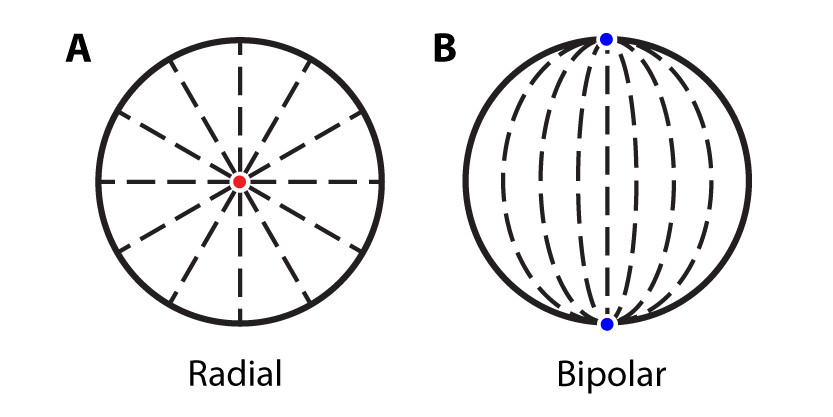
\includegraphics{figures/C2/Ch2-Figs_DropSchem.png}
  \caption{Nematic liquid crystal confined to a spherical volume.
  (A), The classic radial director configuration found under homeotropic boundary conditions.
  The defect is indicated by ${\color{red} \bullet}$.
  (B), The classic bipolar director configuration found under degenerate planar boundary conditions.
  The 2 defects are indicated by ${\color{blue} \bullet}$.}\label{f:2-DropSchem}
\end{figure}

\begin{figure}[h]
  \centering
  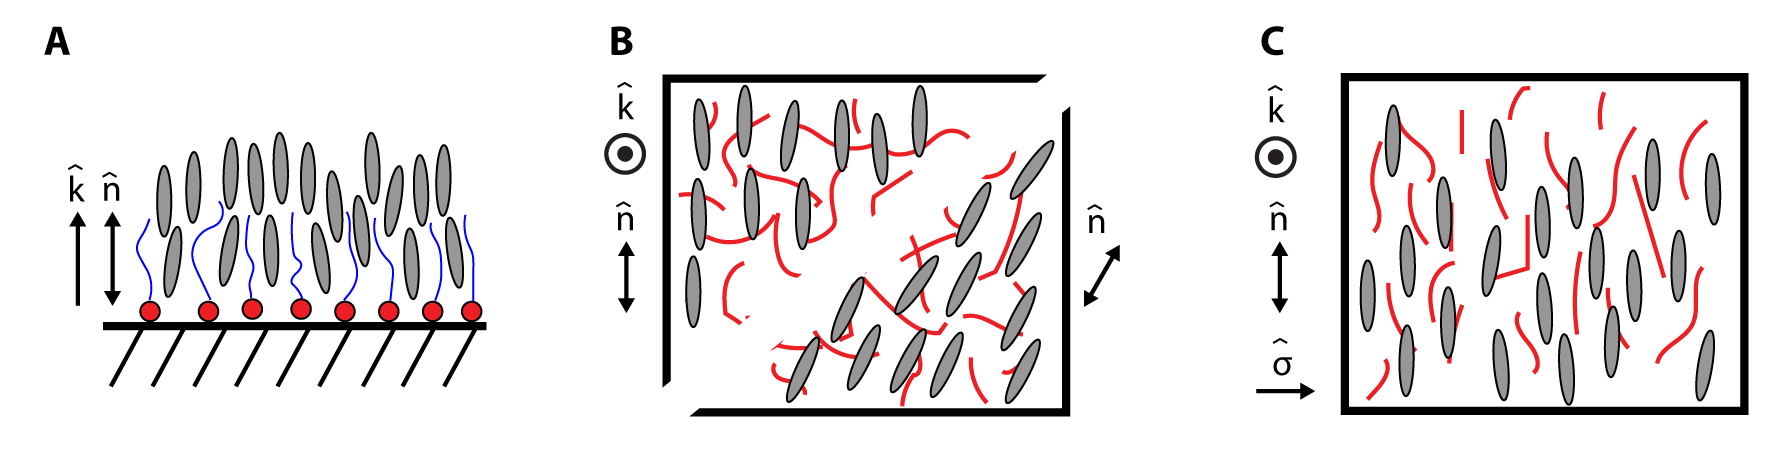
\includegraphics{figures/C2/Ch2-Figs_Anchor.png}
  \caption{Common anchoring schemes for nematic liquid crystals. (A), Homeotropic anchoring enforced by surfactant molecules.
  The polar heads of the molecules adsorb to the substrate, with the nonpolar tails extending into the NLC.
  The tails serve to align the nematic mesogens along the surface normal, making $\mathbf{k} \parallel \mathbf{n}$, as seen in the schematic.
  (B), Degenerate planar anchoring enforced by randomly oriented polymers on the substrate. The polymers only require that the mesogens lie in the plane of the interface such that $\mathbf{k} \perp \mathbf{n}$. Since there is no preferred direction in the plane of the substrate, the mesogens are free to choose any director in the plane, as depicted in the schematic.
  (C), Planar anchoring enforced via aligned polymers on the substrate. Here, the polymers have an alignment direction, setting the direction that the NLC mesogens also prefer to align along, such that $\mathbf{n} \parallel \bm{\sigma}$, where $\bm{\sigma}$ is a vector describing the polymer alignment direction, as defined in the schematic.}\label{f:2-Anchor}
\end{figure}

In an experiment, confinement takes place with either solid boundaries, such as glass cells and capillaries, or fluid boundaries such as in emulsions of a nematic material dispersed in an outer immiscible liquid phase.
It is also possible to confine a nematic using both solid boundaries and fluid boundaries, as with a droplet of NLC sitting on a solid base.
In such a sessile drop, the solid boundary provides a flat base for the NLC;\@ however, the remainder of the confinement is provided by the free surface, where the NLC is in contact with air.
In general, a NLC in contact with an arbitrary boundary will be subject to degenerate tilt boundary conditions.
Thus, for experiments that require a specific boundary condition we must treat the interface.\\

In order to discuss specific strategies for enforcing anchoring, we must first narrow down the compounds that might be used.
NLC can be divided into two broad categories, thermotropics and lyotropics~\cite{RN33}.
In thermotropic LC's, temperature is an important control parameter.
If the temperature is too high, the nematic phase will melt to the isotropic phase and if the temperature is too low, the nematic phase will phase transition to a less symmetric LC phase or to a crystalline phase.
Lyotropic LC's are suspensions of particles in a solvent and therefore are sensitive to both concentration as well as to temperature.

In this Thesis, we will primarily use 4-cyano-4'-pentylbiphenyl (5CB), a thermotropic liquid crystal whose mesogens are $\sim 2$ nm long~\cite{RN33}.\@
5CB belongs to the cyanobiphenyl family of NLC, which are characterized by a cyano (CN) group  bonded to a biphenyl (C$_6$H$_4$)(C$_6$H$_4$) group bonded to an alkyl group of given length, C$_p$H$_{2p+1}$, where $p$ is the number of carbon atoms in the group~\cite{RN33}.
In the case of 5CB, the chemical formula is: (CN)(C$_6$H$_4$)(C$_6$H$_4$)(C$_5$H$_{11}$).
Thus, we see that the ``5'' in 5CB refers to the number of carbon atoms in the alkyl group.
Since the different cyanobiphenyls generally only differ in the number of carbon atoms in the alkyl group, the anchoring techniques we cover below for 5CB are general and should apply to any $p$CB.

To enforce homeotropic anchoring for 5CB against a smooth, isotropic solid boundary such as a glass capillary or glass slide, it is common to either deposit surfactant molecules or bond silanes to the surface.
In both cases, the smooth surface becomes decorated with long chains that stick up normal to the surface.
The nematic mesogens at the surface are aligned by the chains, enforcing homeotropic anchoring at the surface~\cite{RN33}, as seen schematically in Figure~\ref{f:2-Anchor}(A).
For example, to enforce homeotropic anchoring for 5CB on glass, we dip coat glass slides in a $0.1$\% w/w lecithin in hexane solution and then let the slides dry.
When the hexane evaporates, the polar head of the lecithin molecule is attached to the glass surface, leaving the long tails sticking up from the glass~\cite{RN140}.

Similarly, it is common to enforce homeotropic anchoring in solution again using surfactants.
Here, for an organic NLC dispersed in an aqueous phase, the polar head of the surfactant sits in the aqueous phase while the hydrophobic tail inserts itself into the NLC volume, aligning the NLC at the interface~\cite{RN150,RN235}.
For example, we use sodium dodecyl sulfate (SDS) in water to enforce homeotropic anchoring in 5CB emulsions and liquid bridges.
While homeotropic anchoring can be enforced with as little as 1 mM SDS in H$_2$O, we use a solution of 8 mM SDS in H$_2$O for the strongest possible anchoring~\cite{RN235}.
At concentrations above 8 mM, SDS forms micelles in H$_2$O such that working with higher concentrations does not yield any more free SDS in the solution that could potentially adsorb to the interface and contribute to a larger anchoring strength~\cite{RN234}.
This concentration is known as the critical micelle concentration (CMC) and is a common feature in solutions of surfactants or other amphiphilic molecules~\cite{RN233,RN234}. \\

While smooth, isotropic solid boundaries can exhibit degenerate planar anchoring, in general the anchoring will be degenerate and tilted.
Thus, surface is often coated with a polymer such that the polymer orientations on the surface are random.
Since the polymers have no preferred alignment in the plane of the surface, the mesogens are free to choose their own director in the plane~\cite{RN313}, as seen schematically in Figure~\ref{f:2-Anchor}(B).

If a preferred anchoring direction in the plane, $\bm{\sigma}$, is desired, the polymer coating can be rubbed along $\bm{\sigma}$, aligning the polymers and creating ``grooves'' in the polymer coating along the rubbing direction, as seen schematically in Figure~\ref{f:2-Anchor}(C).
The NLC will the align along the rubbing direction, breaking the degeneracy in the anchoring~\cite{RN33,}.
Note that rubbed polymer surfaces do not have perfect planar anchoring but rather exhibit a small tilt angle~\cite{RN232}.
Thus, when designing planar-aligned liquid crystalline cells, where the NLC is confined between two parallel plates with planar anchoring, the rubbing direction on the plates will be anti-parallel.
The anti-parallel rubbing aligns the tilt angles at the plates such that the NLC can still form a homogeneously-aligned domain between the plates~\cite{RN232}. \\

For dispersions of organic NLC droplets such as 5CB in a continuous aqueous phase, we add a polymer like PEO or PVA to the aqueous phase~\cite{RN105,RN93}.
The polymer adsorbs to the interface between the NLC and the continuous phase, giving degenerate planar anchoring.
We know of no easy way to break the planar degeneracy in the anchoring when dealing with a liquid-liquid interface.
In addition, we note that even though 5CB exhibits degenerate planar anchoring at the interface with pure water, the addition of a polymer strengthens the anchoring as well as acting to stabilize the emulsion when 5CB droplets are dispersed in H$_2$O~\cite{RN105,RN93}.\\




\subsection{Birefringence and optically polarized microscopy}
Once the nematic is confined in the desired volume with the desired boundary conditions, the most common way to study the sample is with optical polarized microscopy.
This technique takes advantage of the birefringence of the NLC to determine the director in the sample.
For a uniaxial nematic, the index of refraction along $\mathbf{n}$ is known as the ``extraordinary index of refraction'', denoted $n_E$, and the index of refraction perpendicular to $\mathbf{n}$ is called the ``ordinary index of refraction'', denoted as $n_o$.
Since the index of refraction along $\mathbf{n}$ is $n_E$, the director also serves as the optic axis of uniaxial nematics~\cite{RN232}.
The birefringence is defined as $\Delta n = n_E-n_o$~\cite{RN232}.
If $n_E > n_o$, $\Delta n > 0$ and the material has positive birefringence.
Conversely, if $\Delta n < 0$, the material has negative birefringence.
Thus, the index of refraction affecting the incident light on a birefringent material will depend on the polarization of the light relative to $\mathbf{n}$~\cite{RN232}.

While unpolarized light will be unaffected by the birefringent material, in general polarized light will have its polarization state affected.
Consider linearly polarized light incident upon a birefringent material with $n_E$ along $\hat{x}$ and $n_o$ along $\hat{y}$.
If the incident light is polarized along $\hat{x}$ or $\hat{y}$, it will encounter only either the extraordinary index of refraction or the ordinary index of refraction and will leave the birefringent volume with no change in its polarization state.
However, now let the incident light be linearly polarized at $45^o$.
In this case, the incident light can be decomposed into one component along $\hat{x}$ and another component along $\hat{y}$.
Since each component will see a different index of refraction, they will propagate at different speeds, creating a phase difference between the two components of the incident light.

This phase difference is known as the retardation and is given in multiples of $2 \pi$ by $\Gamma = 2 \pi \Delta n \, d / \lambda$, where $d$ is the thickness of the birefringent material, and $\lambda$ is the wavelength of the incident light in vacuum~\cite{RN232}.
For our example of incident light linearly polarized at $45^o$, let $\Delta n \, d = \lambda / 2$ such that $\Gamma =  \pi$.
The light after leaving the sample will now be polarized at $-45^o$, and the birefringent material has the properties of a half-waveplate~\cite{RN232}.
Similarly, if $\Delta n \, d = \lambda$, $\Gamma =  2 \pi$, the birefringent material is a full-waveplate and the output light will be unchanged~\cite{RN232}.\\

\begin{figure}[h]
  \centering
  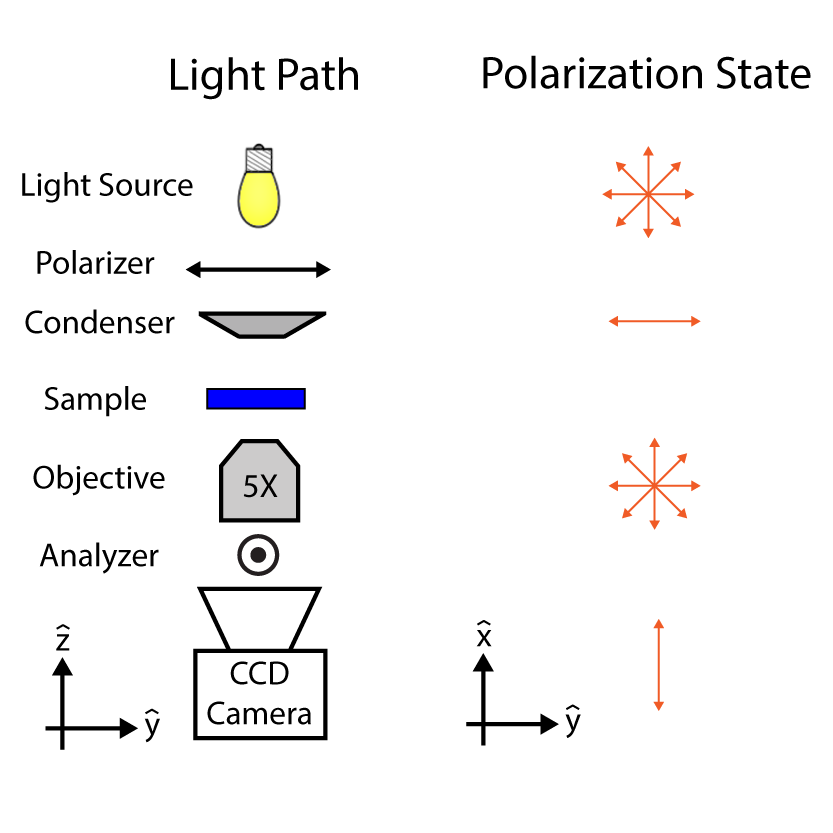
\includegraphics{figures/C2/Ch2-Figs_OPMSchem.png}
  \caption{Schematic of the light path and polarization state for optically polarized microscopy (OPM). OPM places a linear polarizer called the ``polarizer'' before the condenser and another linear polarizer called the ``analyzer'' after the objective. The polarization states depicted in the figure assume the sample is birefringent and the pass axes of the polarizer and the analyzer are orthogonal.}\label{f:2-OPMSchem}
\end{figure}

\begin{figure}[h]
  \centering
  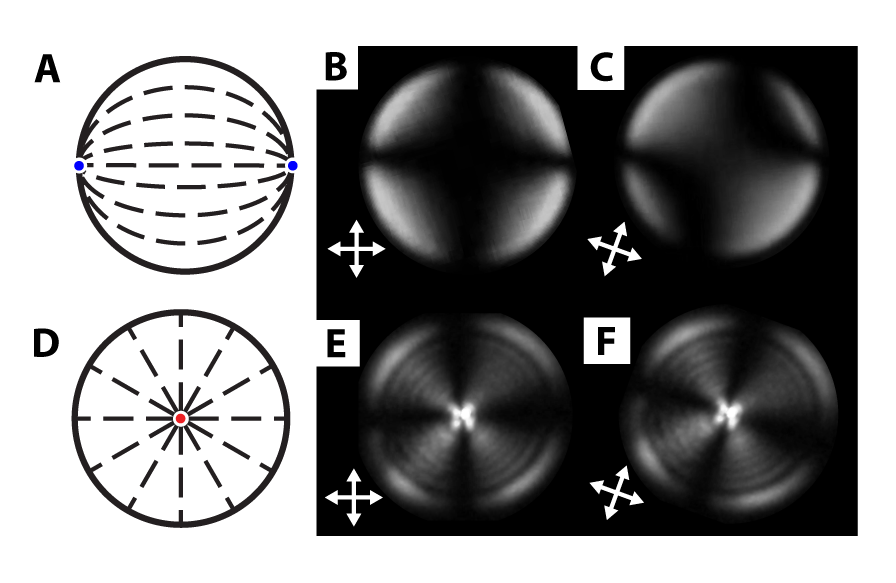
\includegraphics{figures/C2/Ch2-Figs_OPMDrops.png}
  \caption{Example OPM textures for a bipolar drop and a radial drop.
  (A--C), schematic and textures for a radial drop.
  The textures in (B,C) have the polarizer and analyzer directions specified on the images, with the drops oriented as depicted in (A).
  Note how the texture only changes orientation with the polarizer and analyzer orientation, but does not change character.
  (D--F), schematic and texture for a bipolar drop.
  The textures in (E,F) have the polarizer and analyzer directions specified on the images, with the drops oriented as depicted in (D).
  Note how the texture changes as the polarizer and analyzer rotate.
  }\label{f:2-OPMDrops}
\end{figure}

Optical polarized microscopy (OPM) takes advantage of birefringence and turns the change in polarization into changes in transmitted intensity.
The typical setup uses a pair of linear polarizers into the light path of a standard wide-field optical microscope.
A linear polarizer is an optical element that only passes light polarized along a specific axis known as the ``pass axis''~\cite{RN232}.
Thus, unpolarized light incident upon a linear polarizer will have its intensity reduced by half and the output light will be linearly polarized along the pass axis of the polarizer.
Illustrating the light path for optical polarized microscopy, the incident light passes through the first linear polarizer, known as the ``polarizer'', through the sample, through the objective, and through the second linear polarizer, known as the ``analyzer'', before it is incident on the eyepiece or the camera used to capture the microscope image~\cite{RN232}.
The light path is illustrated schematically in Figure~\ref{f:2-OPMSchem}.
If the polarizer and analyzer are ``crossed,'' or oriented with their pass axes orthogonal to each other, any isotropic sample will be entirely dark.
This is because the sample does not affect the polarization state of the incident light such that the linearly polarized light from the polarizer is blocked by the analyzer.
However, if the sample is birefringent, the polarization state of the incident light will change and some of the light will pass through the analyzer and be transmitted onto the eyepiece or camera.
This is illustrated in the schematic in Figure~\ref{f:2-OPMSchem}.

The intensity pattern in the image output from an OPM setup can then be used to deduce information about the sample.
While for our purposes we typically care about the spatial variation of the optic axis, and thus the spatial variation in $\mathbf{n}$, OPM can also be used to determine the birefringence of the sample~\cite{RN232}.
For example, we consider 5CB confined to spherical nematic droplets.
Under homeotropic anchoring the droplet will have the classic ``radial'' director field [see Figure~\ref{f:2-OPMDrops}(A)] while under degenerate planar anchoring the droplet will have the classic ``bipolar'' configuration [see Figure~\ref{f:2-OPMDrops}(D)]~\cite{RN177}.
These configurations can be distinguished by their OPM textures, as seen in Figure~\ref{f:2-OPMDrops}(B,C) for a radial drop and Figure~\ref{f:2-OPMDrops}(E,F) for a bipolar drop.
Note how the light and dark portions of the bipolar texture change from Figure~\ref{f:2-OPMDrops}(E) to Figure~\ref{f:2-OPMDrops}(F) as the polarizer and analyzer change orientation, while still crossed.
The radial texture only rotates with the polarizer and analyzer but does not change in the frame of the polarizer and analyzer; see Figure~\ref{f:2-OPMDrops}(B,C).

\begin{table}[t]
  \centering
\caption{Basic group theory definitions~\cite{RN320,RN319}.}
\begin{tabular}{|r l|}
\hline
{\bf set}:& A collection of objects\\[10 pt]
{\bf group}:& \begin{minipage}[t]{0.65\textwidth}
A set, $\Sigma$, and a binary operation, or group multiplication, $\cdot$, that combines two elements in the set to form a third element in the set, satisfying:
    \begin{itemize}
      \item[]{\bf associativity}: $\forall \; a,b,c \in \Sigma$, $(a \cdot b) \cdot c = a \cdot (b \cdot c)$.
      \item[]{\bf identity}: $\exists! \; e \in \Sigma$ s.t. $\forall \; a \in G, \, a\cdot e=e \cdot a = a$.
      \item[]{\bf invertability}: $\forall \; a \in \Sigma$, $\exists! \; a^{-1} \in \Sigma$ s.t. $a a^{-1} = a^{-1} a = e$, with $e$ the identity.
    \end{itemize}
    If $\forall \; a,b \in \Sigma, \, a \cdot b = b \cdot a$, the group is said to be Abelian.
    Note that the requirement $\forall \; a,b \in \Sigma, \; a \cdot b \in \Sigma$ is known as {\bf closure}.\\
\end{minipage}\\
{\bf Lie group}:& \begin{minipage}[t]{0.65\textwidth}
A group that is also a differentiable manifold, whose group operation is also differentiable. Lie groups are associated with continuous symmetries, for example, SO(3), the set of all rotations in 3D Euclidean space under multiplication. Other common Lie groups include $n$-dimensional Euclidean space $\mathbb{R}^n$ under vector addition, and GL(2), the group of $2 \times 2$ invertible matrices, also under multiplication.\\
\end{minipage}\\
{\bf discrete group}:& \begin{minipage}[t]{0.65\textwidth}
A group whose elements must be countable. This is instantly satisfied if there are a finite number of elements in the group. In this case the order of the group is given by the number of elements in the group. If there are an infinite number of elements, there must be a one-to-one mapping from the elements to the integers.\\
\end{minipage}\\
{\bf homomorphism}:& \begin{minipage}[t]{0.65\textwidth}
A structure-preserving map, $\varphi$, between the groups $G$ and $H$, $\varphi : G \to H$. A homomorphism must satisfy, $\forall \; a, b \in G$, $\varphi(a \cdot b) = \varphi(a) \cdot \varphi(b)$. Since $\forall \; a \in G, \; \varphi(a) \in H$, we see that a homomorphism preserves the group multiplication. A homomorphism is not necessarily a one-to-one mapping. If the homomorphism is one-to-one, then the homeomorphism is an {\bf isomorphism}.\\
\end{minipage}\\
\hline
\end{tabular}
\label{t:2-GroupTheory}
\end{table}


%%%%%%%%%%%%%%%%
% Chapter 3
%%%%%%%%%%%%%%%%

%!TEX root = thesis.tex
\chapter{Active nematics on the surface of a torus}\label{c:3}
\section{Introduction}
Active materials are composed of mesogens that each can convert stored internal energy or ambient energy to kinetic energy, thus driving the material out-of equilibrium~\cite{RN237,RN238,RN40}.
Importantly, this is distinct from global driving mechanisms such as the application of a shear or the imposition of a field; in active materials, the material is driven out-of-equilibrium due to the intrinsic behavior of the constituent particles.
Thus, the materials cannot be understood within the framework of equilibrium statistical mechanics, as the individual particles are subject to forces independent of thermal fluctuations.
Since activity applies to each individual mesogen, the framework of ``active matter'' has been used to study self-organization and self-driven behavior in a variety of systems from flocks of starlings~\cite{RN239,RN240}, collections of robots~\cite{RN241}, colonies of fire ants~\cite{RN242}, cell growth and migration~\cite{RN51,RN160}, and self-propelled particles~\cite{RN168,RN38}.
Note that these examples of active matter span 6 orders of magnitude in size, with behavior such as flocking, giant number fluctuations, chaotic flows, and low-Reynolds number turbulence driven entirely by a single control parameter~\cite{RN237,RN238,RN40}. \\

Much like equilibrium nematics, active nematic materials are composed of individual mesogens that are anisotropic and thus can possess a nematic phase; however, the addition of activity to nematic order brings about an additional contribution to the interaction between the mesogens.
We note that with the exception of bacteria introduced in lyotropic liquid crystals~\cite{RN86}, to date, the majority of experimental and theoretical work on active nematics takes place in 2D.
Thus, to highlight the effect of activity on the nematic mesogens, we consider two active rod-like particles in 2D.
If the active nematic is ``extensile,'' the rods slide past each other; however, if the active nematic is ``contractile,'' the activity drives the rods to slide towards each other.
These interactions result in extensile active nematics being unstable to bend distortions while contractile active nematics are unstable to splay distortions~\cite{RN171,RN170,RN11}.
Thus, the splay and bend instabilities make the homogeneously-aligned director state unstable such that the steady-state of an active nematic is often turbulent~\cite{RN7} and full of pairs of $s = \pm 1/2$ defects that are continuously created and annihilated~\cite{RN11,RN8,RN3,RN27,RN135,RN86}.
These turbulent dynamics are driven by the $s = +1/2$ defects, where the activity coupled with the polar structure of the $s = +1/2$ defects causes the  $s = +1/2$ defects to act like self-propelled particles, with the propulsion direction depending on the type of activity~\cite{RN11,RN8}.
In contrast, due to the three-fold symmetry of $s = -1/2$ defects, $s = -1/2$ defects are not driven by activity and are only advected by interactions between the defects as well as by interactions with the surface.\\

Recent experimental studies with active nematics yielding self-regulated behaviors such as self-sustained oscillations~\cite{RN9}, spontaneous formation of morphological features such as kinks and protrusions~\cite{RN9,RN3}, and undirected motility~\cite{RN9,RN3} have acted as as stimulus to investigate how biological functionality emerges from the interplay between activity, the geometry of the system, and the structure of the internal phase~\cite{RN160,RN51,RN10}.
In this context, defects in active nematics could be harnessed to achieve life-like functionality, as defects are extremely sensitive to the intrinsic geometry of the space they inhabit.
This is easily seen in the connection between the total topological charge on a surface and the topology of the surface, as expressed in the Poincr\'e-hopf Theorem seen in Eq.~[INTRO].
However, the theory of defects in curved spaces extends this connection beyond topology, predicting that the free-energy of a collection of defects is sensitive to the local geometry through the Gaussian curvature~\cite{RN42}.
Importantly, this implies that even though there have been new discoveries as a result of examining defect structures on spheres~\cite{RN45,RN106,RN26,RN110,RN105,RN76,RN101,RN165}, the Gaussian curvature of a sphere is constant such that the impact of curvature can only enter through the sphere radius.
This is is born out in the size-dependent onset of grain-boundary scars in colloidal crystals on the surface of emulsion drops~\cite{RN26,RN110} and the degeneracy in the orientation of the 4 $s = +1/2$ defects in nematic shells~\cite{RN45}.
Even when considering an active nematic on a sphere and the 4 $s = +1/2$ defects become mobile, the defect dynamics can be explained without any mention of Gaussian curvature~\cite{RN9}. \\

Despite theoretical interest in the interplay between varying Gaussian curvature and topological defects, with few exceptions~\cite{RN84,RN25,RN73,RN81}, there has been little experimental work with defects on surfaces where the Gaussian curvature is non-constant.
More notably, there has been no work where the defects have the option to explore regions with both positive and negative Gaussian curvature.
In this scenario with nematic order, the topological charge is expected to unbind such that $s = +1/2$ defects are attracted to regions of positive Gaussian curvature and $s=  -1/2$ defects are attracted to regions of negative Gaussian curvature~\cite{RN17,RN19,RN22}.
In this chapter we consider a 2D extensile active nematic composed of microtubules driven by kinesin motors fueled by adenosine triphosphate (ATP) on the surface of a torus.
Since the torus has a handle, it has a genus of one and thus according to the Poincar\'e-Hopf Theorem written in Eq.~[INTRO] must have vanishing net topological charge.
We note that a nematic on a torus can satisfy this condition by either being defect-free or by having the same amount of positive and negative charge.
While strong spatial confinement or low activity can suppress the spontaneous formation of defect pairs in an active nematic~\cite{RN9,RN247}, we perform our experiments in the turbulent regime such that the torus is always populated with a sea of constantly moving $s = \pm 1/2$ defects that are dynamically created and annihilated.\\

Despite such chaotic and highly nonequilibrium dynamics, we find that on average, topological defects unbind and segregate in regions of oppositely-signed Gaussian curvature.
Notably, due to the chaotic dynamics and the averaging process, the topological charge ceases to be a discrete variable and instead approaches a continuous distribution.
In addition, contrary to equilibrium predictions~\cite{RN36,RN19,RN22,RN20,RN78}, we find that this active unbinding depends only on the local geometry and is independent of the system size and aspect ratio.
When also consider the defect species themselves and find that the average defect density depends inversely on Gaussian curvature over the majority of the toroidal surface, deviating only near the inside and outside of the handle.
Interestingly, near the inside and outside of the handle, we see that the defects themselves, on average, begin to exhibit orientational order.
While $s = +1/2$ defects have been shown to order themselves into a nematic phase in flat space, we find that the $s = +1/2$ defects on a torus exhibit polar order instead~\cite{RN27,RN6}.
We perform our studies with two different ATP concentrations and thus 2 different activities and find that the defect unbinding, the defect density, and the orientational order of the defects all depend on activity.
A numerical integration of the equation of motion of active nematic defects~\cite{RN11,RN8,RN9} performed by Luca Giomi and Dan Pearce at the University of Leiden confirms our experimental results, and further illustrating that the defect unbinding can even be suppressed in the limit of high activity.
Furthermore, by using topological defects as micro-rheological tracers and quantitatively comparing our experimental and theoretical results, we are able to estimate the Frank elastic constant, the active stress, and the defect mobility of a microtubule-kinesin active nematic liquid crystal.
Overall, out results not only confirm the theory of topological defects on curved surfaces, but also demonstrate the surprising phenomenology that arises from adding activity to the interplay between geometry, topology, and order. Out work thus provides insights into the physics of partially ordered active matter and introduces a new avenue for the quantitative mechanical characterization of active fluids.\\


\section{Making active nematic toroids}
\subsection{Active nematic formulation}
We use the mictotubule-kinesin active nematic system pioneered by the Dogic Group at Brandeis University as published in references~\cite{RN3,RN27,RN9,RN135,RN134}.
Microtubules are long, hollow rods that self-assemble from dimers of the $\alpha$- and $\beta$-tubulin proteins~\cite{RN248}.
The $\alpha$/$\beta$-tubulin dimers polymerize end-to-end to form long chains that then polymerize laterally to create cylindrical structures with a helical wrapping of $\alpha$- and $\beta$-tubulin chains~\cite{RN248,RN249}.
This structure gives microtubules a polarity with the (+) end associated with the exposed $\beta$-tubulin subunits and the (-) end associated with the exposed $\alpha$-tubulin subunits~\cite{RN248,RN249}.
While the microtubules serve as the mesogens of the active nematic, the activity comes from kinesin motor proteins bound in clusters to a streptavidin protein.
When in contact with a microtubule, kinesan ``walks'' along the microtubule in discrete steps from the (-) end towards the (+) end, hydrolyzing one ATP molecule into an adenosinediphosphate (ADP) molecule for every 8 nm step~\cite{RN250}.
Thus, a kinesin cluster in contact with two antiparallel microtubules will produce a sliding motion between the two microtubules as the motion of the kinesin motors on the microtubules will displace the two microtubules in opposite directions~\cite{RN4,RN3}.
Conversely, a kinesin cluster in contact with two parallel microtubules will simply walk along both microtubules in the same direction and thus produce no relative motion between the microtubules~\cite{RN4,RN3}. \\

Apart from the activity provided by the kinesin motors, the dominant interaction between the microtubules in an active nematic solution is the depletion interaction~\cite{RN251}, introduced via the presence of poly(ethylene glycol) (PEG, 20 kDa) as a depletant.
The depletion interaction ``bundles'' the microtubules together to form filaments that continuously grow due to the extensile interaction between microtubules provided by the kinesin motors~\cite{RN244,RN4,RN3}.
When the concentration of filaments in the active nematic solution is large enough, the filaments form a viscoelastic network~\cite{RN253,RN3}.
This network inhibits the growth of the filaments such that the filaments buckle at a critical length scale~\cite{RN253,RN3} and fracture into smaller fragments that recombine with other filaments, starting the growth-and-buckling process anew.
In the presence of a liquid-liquid interface, the depletion interaction drives the filaments to the interface between the active nematic solution and outer phase, increasing the concentration such that the filaments locally align and undergo a transition to the nematic phase~\cite{RN3,RN135,RN134}.
Thus, the filament direction serves as the director for the 2D active nematic localized to the interface.
We note that the growth-and-buckling phenomenology of the active filaments is a physical consequence of the extensile dynamics and in the nematic phase is directly responsible for the bend instability and associated defect formation in the  microtubule-kinesin active nematics.
As the filaments buckle and fracture, an $s = +1/2$ and $s = -1/2$ defect pair is produced, with the defects nucleating at opposite ends of the fracture line~\cite{RN3,RN11}.
Hence, with microtubules, kinesin-streptavidin complexes (K/SA), ATP, a depletant, and a liquid outer phase, we have the essential ingredients for an active nematic.\\

However, there are many more compounds in an active nematic solution that serve to enable measurements~\cite{RN3,RN135}, prolong activity~\cite{RN3,RN135}, and allow for a silicone-based outer phases~\cite{RN135}.
The microtubules are fluorescently labeled such that the active nematic can be imaged with fluorescence or fluorescence confocal microscopy.
To prevent photobleaching and phototoxicity during imaging, the active solution contains trolox (Sigma, 238813) and two anti-oxidant solutions.
Anti-oxident solution 1 (AO1) is composed of glucose and dithiothreitol (DTT) and Anti-oxident solution 2 (AO2) is composed of glucose oxidase (Sigma, 238813) and catalase (Sigma, C40).
The active solution also includes an ATP regeneration system to keep the ATP concentration in an active nematic solution constant.
This system is driven by the enzyme mixture pyruvate kinase/lactate dehydrogenase (PK/LDH, Sigma, P-0294) which consumes phoshoenol pyruvate (PEP) to convert ADP to ATP at a rate faster than the K/SA hydrolyzes ATP to ADP~\cite{RN246}. \\

We note that when driven the the liquid-liquid interface, the active filaments do not ever contact the outer phase.
Instead, the interface is packed with a suitable surfactant such that the active nematic filaments deplete to the polar portion of the surfactant molecule.
In fact, the surfactant is then moved along the interface by the motion of the active filaments such that the viscosity of the outer oil phase significantly affects the dynamics of an active nematic~\cite{RN135}.
For a silicone-based outer fluid, we include the triblock copolymer Pluronic F127 (F127) composed of 2 hydrophilic PEG block attached to a central hydrophobic poly(propylene oxide) (PPO) block like PEG-PPO-PEG~\cite{RN252} to the active solution.
Finally, the solution is buffered using a specially designed microtubule buffer (M2B) to keep the enzymes and the motors in their preferred environments~\cite{RN3}.\\

For an experiment, we build the active nematic solution from stock solutions.
The stock solutions in their given compositions are {\bf bolded} such that PEP refers to the general compound while {\bf PEP} refers to the stock concentration/formulation as defined below:
\begin{itemize}
  \item[]{\bf M2B}: 80 mM 1,4-piperazinediethanesulphonic (PIPES) buffer~\cite{RN243} +2 mM MgCl$_2$ + 1mM egtazic acid (EGTA), pH 6.8
  \item[]{\bf PEP}: 200 mM in {\bf M2B}, pH 6.8.
  \item[]{\bf PK/LDH}: Used as purchased.
  \item[]{\bf ATP}: 50 mM in {\bf M2B}, pH 6.8
  \item[]{\bf DTT}: 0.5 mM in {\bf M2B}, pH 6.8
  \item[]{\bf trolox}: Used as purchased.
  \item[]{\bf MIX}: 67 mM MgCl$_2$ in {\bf M2B}
  \item[]{\bf PEG}: (20 kDa) 6\% w/w in {\bf M2B}
  \item[]{\bf F127}: 12\% w/w in {\bf M2B}
  \item[]{\bf glucose}: 300 mg/mL in 20 mM K$_2$HPO$_4$ + 70 mM KCl (pH 7.2)
  \item[]{\bf glucose oxidase}: 20 mg/mL in 20 mM K$_2$HPO$_4$ (pH 7.5)
  \item[]{\bf catalase}: 3.5 mg/mL in 20 mM K$_2$HPO$_4$ (pH 7.4)
  \item[]{\bf K/SA}: 0.175 mg/mL K401 + 0.1 mg/mL streptavidin (Invitrogen, S-888) + 12.5 mM imidazole (pH 6.8) + 1 mM MgCl$_2$ + 0.75 mM DTT + 12.5 mM ATP in {\bf M2B}. K401 consists of 401 amino acids of the N-terminal motor domain of \emph{D.~melanogaster} kinesin purified as previously published~\cite{RN3}.
  \item[]{\bf MT}: 8 mg/mL tubulin labeled with AlexaFluor 647 at 28\% labeling efficiency in {\bf M2B}. Tubulin was purified as previously published~\cite{RN243}.
\end{itemize}
The stock solutions were prepared by the Dogic Group at Brandeis and then shipped to Georgia Tech.
We pipetted the stock solutions as received into aliquots suitable to make 100 $\upmu$L of active nematic solution.
The aliquots are stored in a freezer at $-80^o$ C to prevent degradation of the active compounds.
Prior to each experiment, we remove a set of aliquots from the freezer, quickly thaw the aliquots to room temperature by holding them in our closed hands, and then place all the aliquots on ice except for the MT aliquot.
We leave the MT aliquot out at room temperature so that the tubulin can self-assemble into microtubules.
The polymerization of microtubules is temperature-dependent, with tubulin polymerizing to form microtubules at room temperature and microtubules depolymerizing into tubulin at low temperature~\cite{RN3}.
We then make the initial mixtures and the pre-solution according to the recipe in Table~\ref{t:3-recipe}, leaving the pre-solution on ice.
We wait at least 90 minutes after bringing the MT aliquot to room temperature before mixing the MT with the pre-solution to form the final active nematic solution as specified in Table~\ref{t:3-recipe}.
Note that we bring the pre-solution to room temperature before adding in the microtubules such that the microtubules do not depolymerize when they are added to the pre-solution.
Once we mix the final solution together, we perform our experiments and observe the active nematic until the activity ceases.

\begin{table}[ht]
  \centering
  \caption{Recipe for 100 $\upmu$L active nematic solution}
  \begin{tabular}{|r l|}
    \hline
    \multicolumn{2}{|c|}{Initial mixtures}\\
    \hline
    A01 & 1.5 $\upmu$L {\bf DTT} + 1.5 $\upmu$L {\bf glucose} \\
    A02 & 1.5 $\upmu$L {\bf glucose oxidase} + 1.5 $\upmu$L {\bf catalase} \\
    ATP2 & 2 $\upmu$L {\bf ATP} in:\\
    & \quad 18 $\upmu$L {\bf M2B} for a 10x dilution.\\
    & \quad 38 $\upmu$L {\bf M2B} for a 40x dilution.\\
    \hline
    \multicolumn{2}{|c|}{Pre-solution}\\
    \hline
    2.21 $\upmu$L & A01\\
    2.21 $\upmu$L & A02\\
    2.83 $\upmu$L & ATP2\\
    2.83 $\upmu$L & {\bf PK/LDH} \\
    4.83 $\upmu$L & {\bf MIX}\\
    10.00 $\upmu$L & {\bf trolox}\\
    13.33 $\upmu$L & {\bf PEP}\\
    13.33 $\upmu$L & {\bf PEG}\\
    16.67 $\upmu$L & {\bf F127}\\
    6.67 $\upmu$L & {\bf K/SA}\\
    8.40 $\upmu$L & {\bf M2B}\\
    \hline
    \multicolumn{2}{|c|}{Active nematic solution}\\
    \hline
    83.33 $\upmu$L & Pre-solution (full volume is 83.33 $\upmu$L)\\
    16.67 $\upmu$L & {\bf MT}\\
    \hline
  \end{tabular}
  \label{t:3-recipe}
\end{table}


\subsection{Flat sample confirmation}
Upon receiving the stock solutions, we first made a bulk active gel according to the procedures published in ref.~\cite{RN3} to confirm the integrity of the solutions through the shipping process.
To make a gel, we have to construct a sample chamber where the depletion interaction cannot drive the bundles to aggregate on the walls of the chamber.
We build the sample chamber from a glass coverslip attached via two-sided tape to a microscope slide to form a rectangular channel, as previously published~\cite{RN3}.
Prior to construction, we coat the coverslip and microscope slide with polyacrylamide brushes such that the PEG can penetrate between the brushes, keeping the depletion interaction from driving the active filaments to the surface, where they would adsorb to the glass~\cite{RN3}.
We coat the coverslip and microscope slide according to the published protocol~\cite{RN3}, reproduced below:\\
{\bf Washing slides}
\begin{enumerate}
  \item Place glass into Alconox or Hellmanex solution (prepared per manufacturer specifications)
  \item Sonicate the container for 5 -- 10 minutes.
  \item Rinse the glass with pure water until there are no bubbles (7 -- 10 rinses)
  \item Place glass into a $\geq 70$\% solution of ethanol.
  \item Sonicate the container for 5 -- 10 minutes.
  \item Rinse glass with pure water 5 -- 7 times.
  \item Ensure that water does not bead up on the cleaned glass. If it does, the glass must be washed again.
  \item Place slides into 0.1 M NaOH solution
  \item Sonicate the container for 5 -- 10 minutes.
  \item Rinse glass with pure water 5 -- 7 times.
  \item Store in pure water
\end{enumerate}
{\bf Silane coating for acrylamide polymerization}
\begin{enumerate}
  \item Remove cleaned glass from water, dry with compressed air, and place in a dry container.
  \item Determine the volume of solution needed to cover the glass
  \item Prepare silane-coupling solution ({\bf Solution is unstable. Prepare right before use}):
  \begin{itemize}
    \item 98.5\% v/v Ethanol (200 Proof)
    \item 1.0\% v/v Acetic Acid
    \item 0.5\% v/v 3-(trimethoxysilyl)propyl methacrylate
  \end{itemize}
  \item Cover the glass with the silane-coupling solution and leave it for 10 -- 15 minutes.
  \item Rinse with pure water 5 -- 7 times
\end{enumerate}
{\bf Acrylamide polymerization to silane-coated glass}
\begin{enumerate}
  \item Create or locate stock solution 10\% w/v Potassium Persulfate (KPS) in water
  \item Determine the volume of acrylamide solution needed to cover the glass
  \item Create solution of 2\% w/v acrylamide in water
  \item Degass acrylamide solution under vacuum for 15 -- 30 minutes
  \item To the acrylamide solution add 10 $\upmu$L 10\%KPS solution per 1 mL of acrylamide solution and gently mix.
  \item To the acrylamide solution add 2.5 $\upmu$L TEMED per 1 mL of acrylamide solution and gently mix.
  \item Pour acrylamide solution over coverslips immediately after mixing in the TEMED.
  \item Wait 2 -- 3 hours for polymerization.
  \item Let sit in container until ready to use ({\bf Use within weeks}).
  \item To use, remove glass from container, rinse with pure water, and air dry.
\end{enumerate}

To make the rectangular sample chambers from the polyacrylamide-coated glass, cut strips of 2-sided tape such that the are $\approx1$ mm wide and longer than the coverslip.
Affix the tape strips to the microscope slide in parallel with $\approx 2$ mm between the edges of adjacent strips.
Stick the coverslip onto the tape to create a parallel series of rectangular channels.
Press firmly such that the tape is firmly adhered to both the coverslip and the glass.
Fill the channels with the active nematic solution using capillary action.
Finally, seal the ends of the channel with epoxy.
The samples are now ready to be imaged using fluorescence or fluorescence confocal microscopy. \\

We confirmed that the stock solutions received produced a solution with fluorescent active filaments that grew and fractured.
The activity in the gel sample appeared constant for the entirety of its  $\approx 24$ hr lifespan.
The observed behavior qualitatively agreed with previously published behavior by the Dogic group~\cite{RN3}.


\subsection{Making toroidal droplets}
With the integrity of the active solution confirmed, we turn to making stable toroidal droplets with our active solution.
We generate our toroidal droplets following the procedure detailed in Refs.~\cite{RN29,RN47,RN257}.
Briefly, the setup consists of a rotating stage holding a cuvette containing the continuous, or outer phase, and a syringe holding the dispersed, or inner phase connected to a needle inserted into the cuvette.
We control the angular velocity of the rotation $\omega$, by driving the rotating the stage with a motor powered by a constant voltage source.
We control the position of the needle in the cuvette with a micromanipulator and we control the flow rate and volume of the inner phase with a syringe pump.
In addition, we place a camera below the rotation stage such that we can image the droplet generation process.
We insert the needle into the cuvette offset from the center of rotation such that pumping the inner phase into the cuvette while the cuvette is rotating will generate a curved jet.
Provided that we rotate fast enough such that the curved jet closes upon itself before it undergoes breakup, we form a toroidal droplet.
This condition is a balance of two timescales: (i) the timescale required to undergo breakup, $t_b \approx \mu_o a_{jet} f(\mu_i/\mu_o)/\gamma$, where $\mu_o$ is the viscosity of the outer phase, $\mu_i$ is the viscosity of the inner phase, $a_{jet}$ is the radius of the jet, and $\gamma$ is the interfacial tension between the inner and outer phases; and (ii), the timescale required to close the curved jet onto itself, $T = 2\pi/\omega = 2 \pi R_{tip}/U$, where $R_{tip}$ is distance from the center of rotation the the needle and $U$ is the linear velocity of the continuous phase at the needle.
Equating the two timescales and rearranging terms allows us to express this condition in terms of the Capillary number of the outer phase like $\textup{Ca}_o > (2 \pi / f(\mu_i/\mu_o))R_{tip}/a_{jet}$ ,where $\textup{Ca}_o = \mu_c U/\gamma$ a dimensionless group comparing the viscous stresses to the surface tension stresses.
We note that $a_{jet} \approx a_{tip}$, the radius of the needle.
Experimentally, it has been found that $\textup{Ca}_o > 2.2 R_{tip}/a_{tip}$ for $\mu_o = 5000$~mPa~s and $\mu_i = 1$~mPa~s in order to form a torus~\cite{RN29}.
In practice, we simply look at the video of the process to verify that our chosen parameters generates a jet that closes in upon itself before breaking.
To control the size and aspect ratio of the toroidal droplet, we tune $R_0$ by changing $R_{tip}$ and $a$ through the total injected volume. \\

Toroidal droplets generated in a simple fluid are unstable due to the influence of surface tension.
Surface tension acts to minimize the interfacial area between two immisicble fluid phases, hence the ubiquity and stability of spherical droplets in nature; the sphere minimizes the surface area for a given volume~\cite{RN178}.
The physics behind the surface tension stress at an interface comes through the Laplace pressure $\Delta P$, describing the pressure drop across a fluid-fluid interface~\cite{RN178}:
\begin{equation}\label{e:3-LapPres}
  \Delta P = P_i - P_o = 2 \gamma (- H),
\end{equation}
where $P_i$ is the pressure in the inner fluid phase, $P_o$ is the pressure in the outer fluid phase, and $H$ is the mean curvature of the interface.
Recall that $H = \textup{det}\big \{ \mathbf{L} \big \}$, where $\mathbf{L}$ is the Weingarten Matrix from Eq.~[INTRO]\fxnote{ref INTRO} defined such that the mean curvature of a sphere with radius $r$ choosing an outward-facing normal is $H = -1/r$ everywhere on the surface of the sphere.
Thus, the Laplace pressure tells us that a spherical droplet has greater pressure on the inside than on the outside, and that due to its constant mean curvature, the pressure inside the droplet is also constant such that the droplet is stable.
However, we know that $H$ for a torus varies along the surface such that the pressure inside the torus must also vary.
This intrinsic pressure difference creates the flow inside a fluid torus responsible for the shrinking instability in toroidal droplets, where the handle shrinks smoothly until it closes and the toroidal droplet becomes a spherical droplet~\cite{RN29,RN255}.
In addition, the Laplace pressure can also cause the tube of a toroidal droplet to break up reminiscent of the Rayleigh-Plateau instability such that the toroidal droplet breaks into one or more spherical droplets~\cite{RN29,RN256}.
While the study of the fluid modes in nontrivial topologies is interesting in its own right and has led to interesting insights into fluid phenomena such as charged jets~\cite{RN256} and viscous fingering~\cite{RN254}, we are more concerned with creating a stable toroidal droplet. \\

As the surface tension stress is responsible for destabilizing the toroidal droplet, to stabilize a toroidal droplet we need to counter the surface tension stress.
To do so, we make our toroidal droplets using a yield-stress material as the outer phase~\cite{RN47,RN258}.
Briefly, a yield-stress material has a threshold stress such that the material responds like an elastic solid to imposed stresses less than the yield-stress and flows like a viscous liquid to imposed stresses greater than the yield-stress.
Thus, provided that the yield-stress is greater than the surface tension stress, the toroidal droplet will be unable to transform to a spherical droplet and will be stable indefinitely.
Since the surface tension stress is given by the Laplace pressure, we see that balancing the Laplace pressure and the yield stress, $\tau_c$, will give us a critical radius of curvature, $R_c$, determining the stability of a toroidal drop, $\gamma/\tau_c \sim R_c$.
If the smallest radius of curvature on a toroidal drop is larger than $R_c$, the toroidal droplet will be stable --- generally, the smallest radius of curvature on a torus is the tube radius.
However, for toroids with $\xi \sim 1$, the radius of the handle can be the relevant lengthscale determining the stability of a toroidal droplet.
Since the active nematic solution is aqueous, we use an oil-based yield-stress material, DC-9041 (Dow Corning), a silicone elastomer.
To tune the yield stress, we dilute pure DC-9041 with 10~cSt PDMS oil (Clearco).\
We dilute to 74\%~--~77\% w/w DC-9041 to form stable active nematic toroids with tube radii from 150~$\upmu$m~--~300~$\upmu$m.\\

Making a toroidal droplet in a yield-stress material has some key differences to making a toroidal droplet in a viscous fluid.
Notably, the yield-stress material is only fluid-like in regions where the stress is greater than the yield-stress.
Thus, for best results, we need to pre-shear the yield-stress medium such that the greatest possible volume of yield-stress material is fluidized.
We do this by letting the cuvette rotate with the needle inserted for up to 30 s before we begin pumping the inner liquid into the cuvette.
While a pre-shear is not strictly necessary to form a toroidal droplet, the cross-sections of the tubes of toroidal droplets made with a pre-shear are generally more circular than toroidal droplets made with minimal pre-shear.
This is because the wider the volume of fluidized yield-stress material, the less the pumped volume ``climbs'' up the needle.
In addition, adding a pre-shear generally helps the overall toroidal droplet be more axisymmetric.
We also find that making toroidal droplets close to the free-surface of the yield-stress material helps to reduce climbing, but the physical reason for this is unclear.\\

For general experiments with toroidal droplets where there is a large amount of the inner phase available, we simply fill the syringe with the inner phase.
However, for the active experiments, we have only 100~$\upmu$L of active solution per experiment, which is not enough to even fill the Luer-lock syringe tips we use to connect a syringe to the tubing.
To accommodate the low sample volume, we fill the syringe with mineral oil (xx cSt, XXX)\fxnote{GET MO source} as a dummy fluid and increase the length of the tubing between the syringe and the needle such that the volume of tubing is greater than $100$~$\upmu$L.
We pump the dummy fluid until it fills the tubing, insert the filled tubing into the container holding the active nematic solution, and the withdraw the dummy fluid to pull the active nematic solution into the tubing.
Once the active nematic solution is loaded into the tubing, we make toroids as if it were any other inner phase.
It is important to make sure that the tubing is entirely full of mineral oil such that there is no air at the interface between the dummy liquid and the active nematic solution.
Air bubbles in the tubing will inhibit forming high-quality toroidal droplets as the air bubble acts as a ``spring'' in the fluid system, introducing significant ``lag'' between the start and stop of the syringe pump and the beginning and end of the fluid flow from the needle.
In addition, it is important to withdraw the dummy fluid slowly ($\approx 1$~mL/s) when loading the active nematic solution to prevent an emulsion between the active fluid and the dummy fluid forming in the tube.\\




\section{Imaging active nematic toroids}
Once the active nematic toroidal droplet is made, we let the droplet rest for 2~--4~4~hours to ensure the nematic is fully formed on the surface of the toroidal droplet.
We then image the droplet via fluorescence confocal microscopy (Nikon A1R or Zeiss LSM 700) until the activity ceases.
This typically occurs between 6~--~10~hours after making the toroidal droplet.


\subsection{Confocal fluorescence microscopy}
Unlike traditional wide-field microscopy, confocal microscopy allows us to image individual planes in the image such that we can construct a 3D representation of the sample~\cite{RN260}.
Regardless of the illumination source, confocal microscopy functions by placing an aperture in front of the detector at a confocal plane to the focal plane in the sample~\cite{RN259}.
Thus, only light from the focal plane will pass through the aperture; light from any other plane in the sample will be out of focus in the plane of the aperture and thus will not pass through the aperture.
Typically, the focal plane is changed in the sample by translating the microscope stage up and down.
Since the introduction of scanning confocal microscopy, and especially scanning laser confocal fluorescence microscopy, confocal microscopy has seen widespread adoption and is now a standard technique in multiple fields~\cite{RN261,RN262,RN260}.
Here, the illumination mode is epifluorescent, such that a laser beam is emitted through the objective and incident on a portion of the sample.
The illuminated portion of the sample then fluoresces and the output intensity from the focal plane is recorded.
This process is enhanced with a dichroic mirror and a pair of filters such that both the illumination source and the emitted light pass through the objective, but only the emitted light is passed to the detector.
With a tight laser beam and a set of mirrors to scan the laser beam over the sample, the emitted intensity in the focal plane can be highly localized such that the spatial resolution in the focal plane is set by the size of the laser spot~\cite{RN260}.
This reduces the impact of photobleaching, but more importantly allows the user to `zoom'' into the sample without changing the objective magnification simply by changing the size of the laser spot and detector optics such that a smaller scan area with higher spatial resolution in a given focal plane still illuminates the entire detector.
We note that the $z$-resolution between focal planes is still set by the diffraction limit of the emitted light, such that the only way to meaningfully improve the $z$-resolution is to change the objective.
Coupling confocal microscopy to fluorescence microscopy not only improves signal-to-noise ratio, but also allows us to selectively image only the dyed portion of the sample.
In our case, this corresponds to imaging only the active filaments.
Thus, we can acquire a 3D image stack showing only the active nematic depleted to the toroidal surface.


\subsection{Confocal setup and parameters}
Both of the confocals we use are scanning laser confocal microscopes.
Procedurally, both microscopes scan the image plane with a focused laser beam while recording the output intensity, adjust the height of the stage to change the focal plane, and then repeat the process until the image stack is acquired.
While the image stack can be thought of in terms of 3D voxels, the $z$-resolution between focal planes is less than the $xy$-resolution in the focal plane such that it is more convenient to think of the image acquisition as a stack of 2D images.
We note that we are inherently restricted to only imaging the lower half of the toroidal droplet due to refraction effects.
The light emitted from the upper half of the toroidal droplet travels through the aqueous active solution and then is refracted by the curved interface between the active solution and the yield-stress material.
In contrast, the light from the lower portion of the toroid is emitted directly into the yield-stress material such that it's light path is unaffected by refraction.
However, even though we can in principle image up to the midpoint of the torus, in practice we typically stop our image stack below the midpoint.
This is because the time required to adjust the stage height is the slowest portion of the imaging process for both of the confocal microscopes we use.
Since we wish to acquire as many frames as possible to increase the amount of data we have for each toroid, we must must balance the time required to take an image stack versus the size of the image stack.\\

The microtubules are dyed with AlexaFluor 647, which has en excitation peak of 651~nm and an emission peak of 667~nm~\cite{RN264}.
Thus, we use a 633~nm laser as our illumination source and a Cy5 filter set such that only the emitted light reaches the detector.
The Cy5 filter set includes a 590~--~650~nm bandpass excitation filter, a 660~nm longpass dichroic mirror, and a 663~--~738~nm emission filter~\cite{RN263}.
The filters and mirror are designed with steep passband transitions such that the quoted ranges are good representations of the passband.
Note that for illumination with a laser, the excitation filter is unnecessary, but is standard when purchasing the filterset.
The excitation filter is necessary in wide-field fluorescence microscopy when illuminating with a white-light source.\\

While the two confocal microscopes we use operate the same, there are key differences in the detection that affects measurement protocol as we affects the quality of the data.
The Zeiss microscope uses standard photomultiplier tubes (PMT) as the detector.
Unfortunately, standard PMTs do not detect wavelengths above 600~nm well, as the quantum efficiency of the detector decreases with increasing wavelength and is typically below 10\% in that wavelength range~\cite{RN263}.
This means that we have to increase the intensity of the laser, increase the gain on the detector, and even average two scans of each image plane in order to increase the signal-to-noise ratio to an acceptable level.
As a result, data from the Zeiss microscope take longer to collect and the active nematic exhibits mild photobleaching for long acquisitions.
However, we note that the photobleaching is mild enough that it does not appreciably affect our data analysis. \\

In contrast, the Nikon microscope uses a Gallium Arsenide Phosphide (GaAsP) PMT in conjunction with standard PMTs to increase the quantum efficiency of the detector suite for larger wavelengths.
GaAsP PMTs maintain a roughly constant quantum efficiency of $\approx 50$\% up to 700~nm~\cite{RN263}.
Thus, we can keep both the laser power and detector gain low while still only needing a single scan of the image plane to acquire a higher quality image stack than we get from the Zeiss microscope.
We therefore can acquire image stacks with a higher time resolution, a higher image quality, and with no noticeable photobleaching when using the Nikon microscope.\\

We set up a measurement as follow.
First, we place the sample on the microscope stage and and find the droplet by eye using standard brightfield microscopy.
We then set up the confocal such that appropriate laser and filter set are chosen.
Next, we set the microscopes to scan the image plane and display the output in real time.
We move the stage to find the bottom and the sample and then move the stage to determine the highest plane that we will measure.
As a rule of thumb we aim for one image stack to take 30~--~50~s to acquire.
This corresponds to roughly 15~--~25 image planes, depending on the microscope used to acquire the data. \\

Now that we have set up the size of the image stack, we turn to tuning the laser intensity and gain to produce the highest quality images.
We first find the image plane with the brightest intensity, and manipulate the intensity and gain such that at most $\approx 5$\%  of the pixels are saturated.
While a higher laser power and lower gain will produce better quality images, setting the laser power too high can lead to photobleaching for long time measurements.
Thus, we generally keep the gain roughly halfway between the minimum and maximum values and then adjust the laser power accordingly.
If we are on the Zeiss microscope, we set the microscope to scan each image plane twice and average the measurements such that we can reduce the overall laser power to minimize photobleaching.
We then go to the bottom plane and set an offset corresponding to an intensity floor for the measurement.
Pixels with an intensity below the offset are set to 0.
This helps to remove some of the thermal noise in the image; in practice, we have enough signal that this parameter is does not really matter.\\

Once these parameters have been set, we turn on the Perfect Focus System to eliminate the effect of thermal and mechanical drift in the measuring system.
Thermal and mechanical drift in the measuring system means that over time the measured distance between the objective and a given reference plane in the sample will change.
This will result in the physical sample volume imaged by the confocal changing over time.
The Perfect Focus System corrects this by maintaining the distance between a specified reference plane and the objective with incredibly high accuracy.
The microscope then resets its zero to the reference plane before every scan through the image stack and thus will never accumulates error due to drift.
Finally, we set the microscopes to image continuously for 12 hours, starting the next image stack as soon as it finishes the previous stack until the 12 hours have expired.
We note that files imaged for longer than 12 hours can be difficult to open due to their large size, even on the computer associated to the microscope.\\

Once the image acquisition is finished, we crop the raw confocal time series to only include the portion where the toroidal droplet is active.
We save this cropped version in single multi-page \texttt{.tiff} file including the metadata concerning acquisition parameters.
This standardizes the data format between the different microscopes to make it easier to read in to the computer.


\subsection{Passing confocal data into MATLAB}
The core routine to load the image stack into MATLAB comes from the \texttt{bioformats} toolbox put out by the Open Microscopy Environment~\cite{RN265}.
The Open Microscopy Environment maintains the open-source \texttt{OME-TIFF} image format for microscopy data.
The \texttt{bioformats} toolbox allows us to call the imaging parameters such as pixel-to-length conversions, framerate, etc., as well as access the total times series of image stacks as a 3 dimensional array in MATLAB.
The data are stored in image planes in the order they were taken such that the effect is concatenating the time-series of image stacks along the $z$ dimension in the order they were taken.
Thus, to locate a specific image stack you have to know which stack in the time series you want as well as the number of planes in each image stack.
Since the entire image series from the confocal can be up to 8~Gb, we first extract the relevant data and then remove the image series from memory so that we have the ability to analyze the data.\\

We first determine the surface of the toroidal droplet by averaging all the image stacks together and then applying an intensity threshold.
Since we have fluorescence confocal data where the fluorescent media has depleted to the surface of the torus, averaging all of the image stacks together creates a clear intensity image of the toroidal surface as both transient structures in the bulk as well as the filamentary structure of the active nematic is washed out in the averaging process.
We next threshold the data to binarize the image stack and reduce the thickness of the surface in the binary stack.
Since there are a large range of threshold values that do not change the output surface and it is easy to check the result of an applied threshold, we determine this threshold value by hand.
From the binarized 3D array, we look at every $xy$ position and determine the lowest $z$ value that contains a nonzero value.
We take this $z$ value to be the height $h$ of the toroidal surface record it in an array such that we have a Monge parameterization of our surface, $h = f(x,y)$~\cite{RN23}. \\

We next consider the intensity stack for each time point and perform a maximum intensity projection into the $xy$-plane with the caveat that the only consider pixels within $\pm 5$ planes of the height at each individual point.
This process largely prevents transient bright filaments in the bulk from affecting our measurements.
Thus, we now have recorded our surface and reduced our data from a time-series of 3D image stacks to a time-series of 2D images such that we have the intensity $I = f(x,y,t)$.
Finally, we clear the raw confocal data from memory and work to (i), determine the director and defects from the intensity projections, and (ii), calculate the surface curvature and surface normals using $h(x,y$).




\section{Determining director and defects}
In the intensity projection of a confocal stack at a time $t_0$, $\mathbf{n}$ is given by the direction of the microtubule bundles.
This direction is obtained from the greyscale image by finding the direction along which the intensity fluctuates the least for each pixel using a technique called coherence-enhanced diffusion filtering (CEDF)\cite{RN30}.
We illustrate this technique with an example analysis of the intensity projection shown in Figure~\ref{f:3-CEDF2}(A).


\subsection{Coherence-enhanced diffusion filtering}
To begin with, the original intensity image $I = I(x,y,t_0)$ is denoised using a Gaussian blur of standard deviation $\sigma$ and side length $6 \sigma -1$ to lessen contributions to the intensity fluctuations from random noise, giving us the blurred image $I_{\sigma}$.
The result of blurring the example full-stack image as well as the inset isolated defect pair in Figure~\ref{f:3-CEDF2}(A) is seen in the main image and inset of Figure~\ref{f:3-CEDF2}(B), respectively.
This blur was performed using a $5 \textrm{ px} \times 5 \textrm{ px}$ Gaussian filter with $\sigma= 1$ px.\\

Next, the gradient tensor for $I_{\sigma}$ is calculated for each pixel:
\begin{equation}
(\nabla I_{\sigma})(\nabla I_{\sigma})^T =
\begin{bmatrix}
(\nabla_x I_{\sigma})(\nabla_x I_{\sigma}) & (\nabla_x I_{\sigma})(\nabla_y I_{\sigma}) \\
(\nabla_y I_{\sigma})(\nabla_x I_{\sigma}) & (\nabla_y I_{\sigma})(\nabla_y I_{\sigma})
\end{bmatrix}.
\end{equation}
Since the microtubule bundles have head-tail symmetry, we cannot use the gradient vector alone to define the bundle orientation as the vector has a defined head and tail.
The rank-2 gradient tensor is symmetric and is the same whether it is constructed with the gradient vector or the negative gradient vector.
Thus, we use the gradient tensor to ``remove the head'' from the gradient vector.
We now define the coherence direction of a rank-2 tensor as the direction of the eigenvector associated with the smallest eigenvalue.
The coherence direction represents the direction along which the spatial intensity fluctuations are the weakest and is periodic on the interval $[0^{\circ}, 180^{\circ})$.
The coherence direction calculated for the gradient tensor of each pixel for $I_\sigma$ shown in the main image and inset of Figure~\ref{f:3-CEDF2}(B) is seen in the main image and inset of Figure~\ref{f:3-CEDF2}(C), where the orientation of the coherence direction on the interval $[0^{\circ}, 180^{\circ})$ measured CW off of the horizontal axis has been mapped to the greyscale values $[\textrm{black}, \textrm{white})$ .
We see that there are still too many fluctuations in the coherence directions shown in Figure~\ref{f:3-CEDF2}(C) to determine $\mathbf{n}$.\\

The following step seeks to remove small-scale fluctuations in the coherence direction by averaging once more.
Here, we perform a component-wise average of the gradient tensor for each pixel to find the structure tensor for each pixel.
This operation can be written as:
\begin{equation}
K_{\rho} \ast (\nabla I_{\sigma})(\nabla I_{\sigma})^T =
\begin{bmatrix}
K_{\rho} \ast ( \nabla_x I_{\sigma})(\nabla_x I_{\sigma}) & K_{\rho} \ast (\nabla_x I_{\sigma})(\nabla_y I_{\sigma}) \\
K_{\rho} \ast (  \nabla_y I_{\sigma})(\nabla_x I_{\sigma}) & K_{\rho} \ast (\nabla_y I_{\sigma})(\nabla_y I_{\sigma})
\end{bmatrix},
\end{equation}
where $K_{\rho}$ is a Gaussian filter with standard deviation $\rho$, where $\rho$ should be about the size of the relevant coherence feature in the image.
If $\rho$ is too small, the coherence directions of the structure tensor will resemble those from the gradient tensor, while if $\rho$ is too large the desired coherence features will be washed out by the averaging.
The coherence direction of the structure tensor calculated with $\rho = 5$ px and filter size $29\textrm{ px } \times 29$ px for each pixel of $I_{\sigma}$ seen in the main image and inset of Figure~\ref{f:3-CEDF2}(B) is shown in the main image and inset in Figure~\ref{f:3-CEDF2}(D), respectively.
As before, the orientation on the interval $[0^{\circ}, 180^{\circ})$ measured CW off of the horizontal axis has been mapped to the greyscale values $[\textrm{black}, \textrm{white})$.
 We take this output of the coherence direction of the structure tensor for each pixel as the local ``molecular director'' $\mathbf{u}$, representing the local orientation of the active nematic.
\newpage
\begin{figure}[h!]
  \centering
  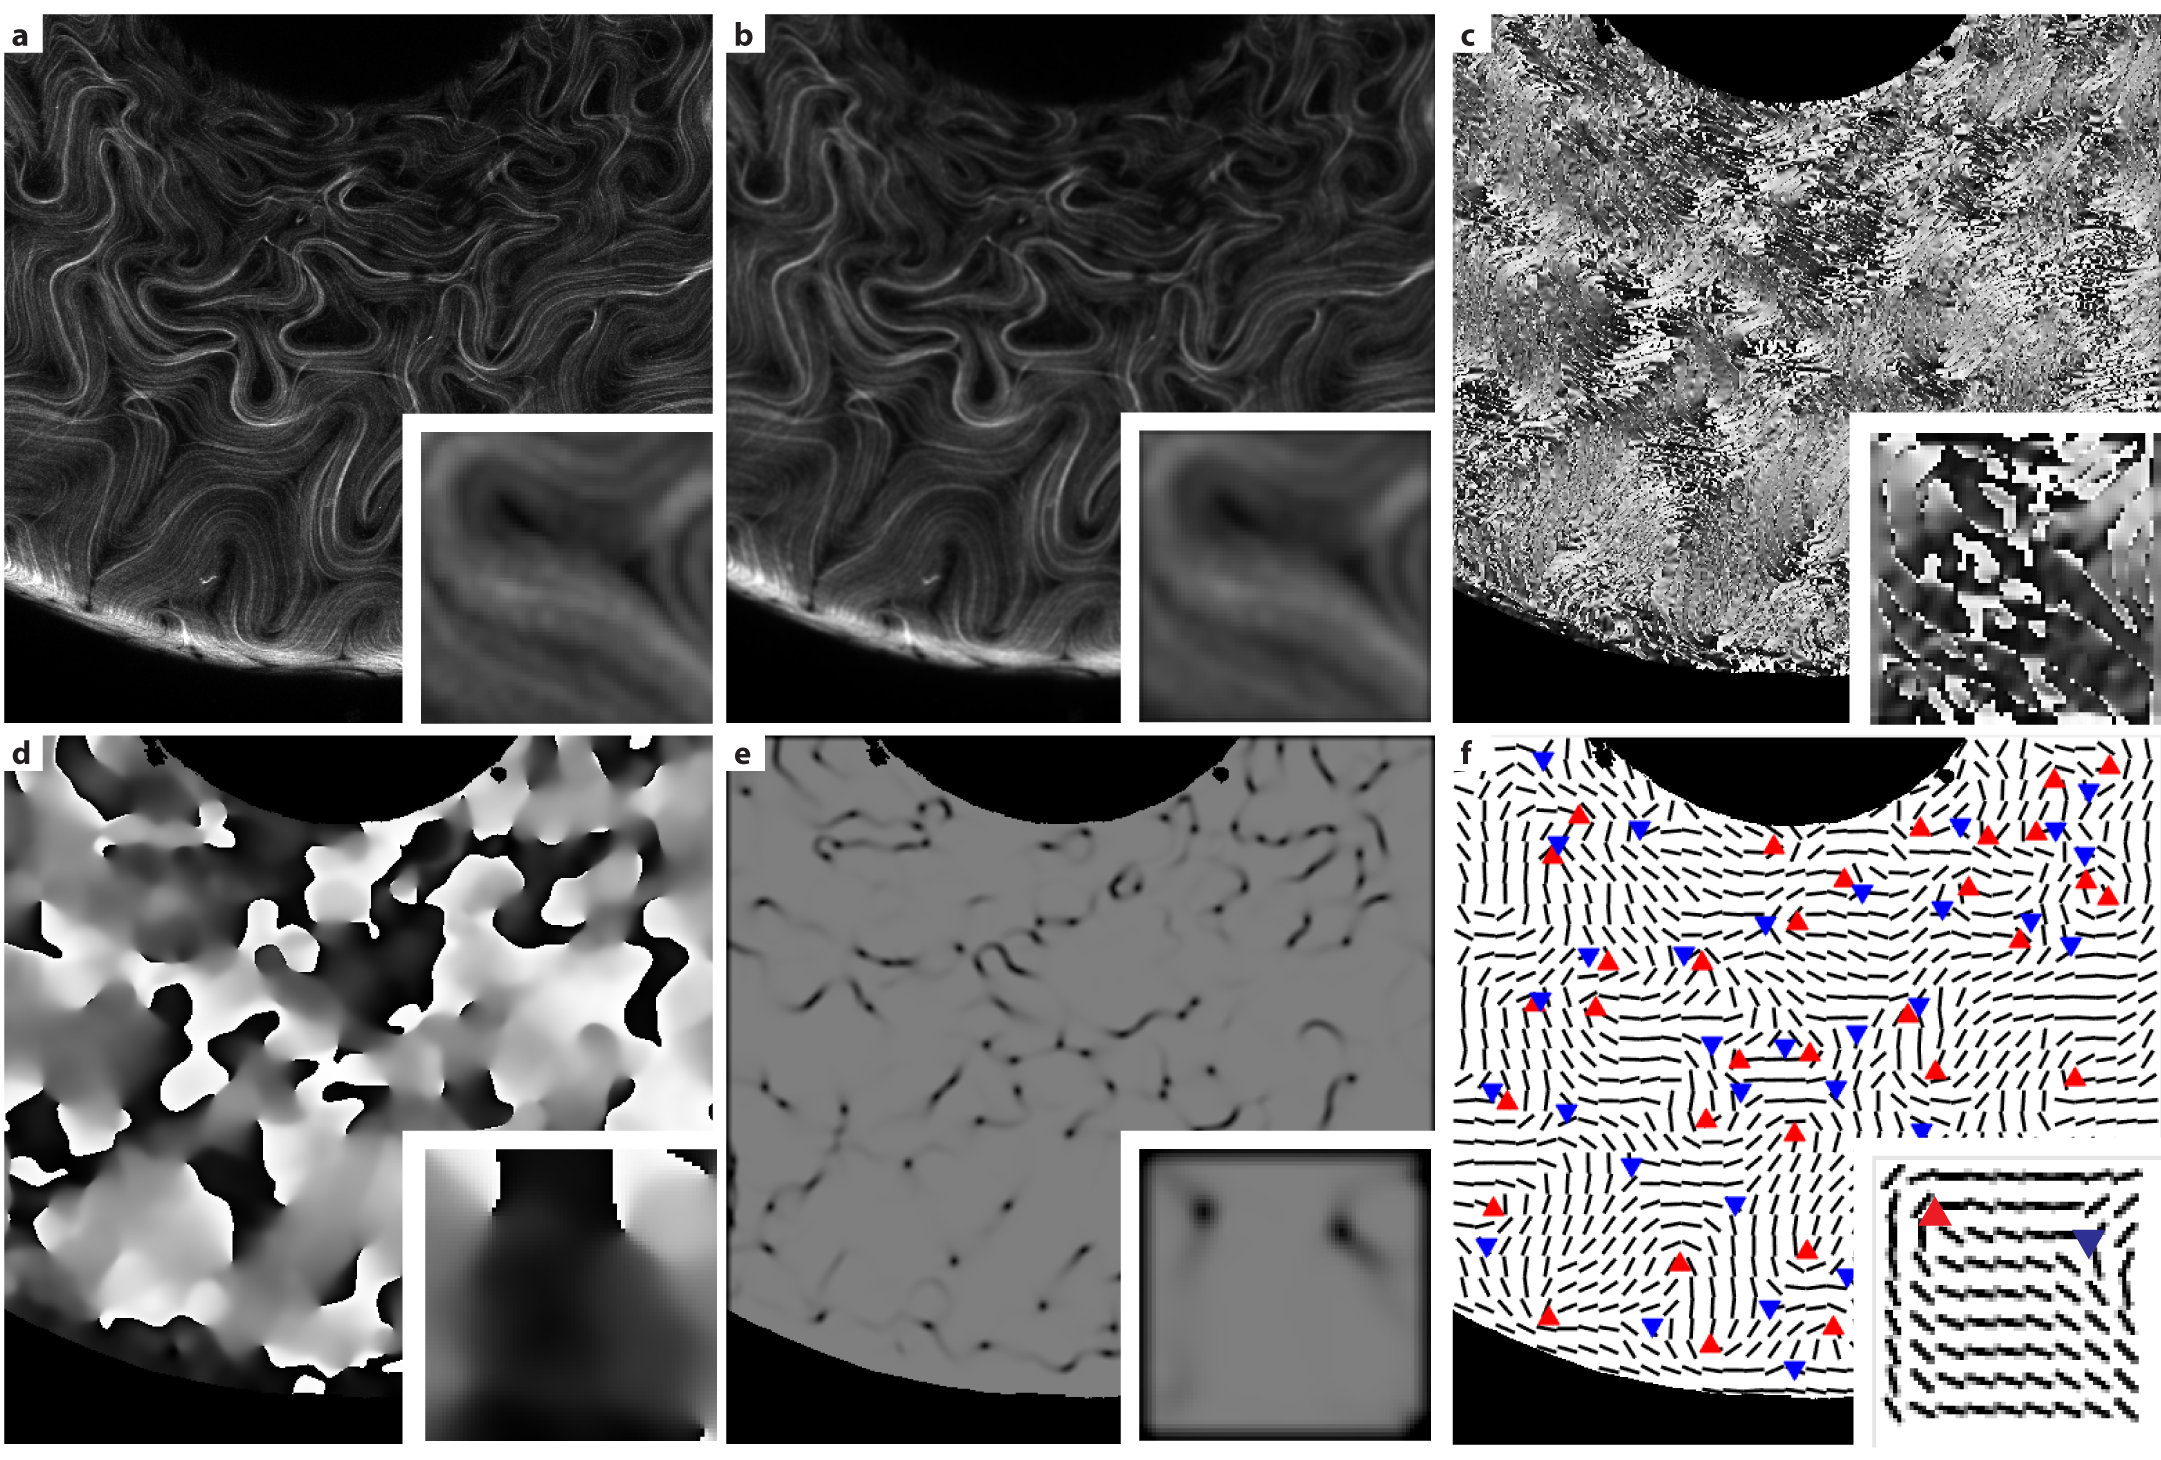
\includegraphics[width=\textwidth]{figures/C3/Ch3-Figs_CEDF2.png}
  \caption{Step-by-step output to find the director and defects from an active nematic image.
(A), Maximum-intensity projection of a confocal stack along $-\hat{z}$ at a single time.
Inset: Close up of a defect pair.
(B), Image from (A) after applying a $5 \textrm{ px} \times 5 \textrm{ px}$ Gaussian blur with standard deviation of 1 px.
Inset: The same operation applied to the image in the inset of (A).
(C), Coherence directions of the tensors formed from the gradient of the image in (B).
Black represents $0^{\circ}$ and white represents $180^{\circ}$ measured CW from the horizontal.
Inset: The same operation applied to the image in the inset of (B).
(D), Coherence directions of the structure tensors formed by component-wise averaging the gradient tensors formed from image (B).
Black represents $0^{\circ}$ and white represents $180^{\circ}$ measured CW from the horizontal.
The averaging is done with a $29 \times 29$ Gaussian filter with standard deviation of 5 px.
Inset: The same operation applied to the image in the inset of (B).
(E), The scalar order parameter $S$ obtained by diagonalizing the $\mathbf{Q}$ formed from the directions in image (D).
$\mathbf{Q}$ is formed for each point by considering the directions of all points in a 5 pixel radius.
Inset: The same operation applied to the image in the inset of (D).
(F), The director obtained by diagonalizing the $\mathbf{Q}$ formed from the direcions in image (D).
$\mathbf{Q}$ is formed for each point by considering the directions of all points in a 5 pixel radius.
The defects are calculated by considering points of low $S$ and calculating the $\mathbf{n}$-rotation along a path encircling the point.
$s = +1/2$ defects are represented by ${\color{red} \blacktriangle  } $  and $s = -1/2$ defects are represented by ${ \color{blue} \blacktriangledown  } $.
Inset: The same operation applied to the image in the inset of (D).}\label{f:3-CEDF2}
\end{figure}
\newpage
\subsection{Calculating the director}
From $\mathbf{u}$, we compute the 2D tensor nematic order parameter defined in Eq.~\ref{e:2-2DOrderRaw}, taking the average over all the $\mathbf{u}$ of all points in a specified radius of the point of interest.
We perform this averaging using a disc filter of radius $\beta$.
We then diagonalize the $\mathbf{Q}$ as shown in Eq.~\ref{e:2-2DOrderDiag}, providing $\mathbf{n}$ and $S$ for each pixel.
For the orientations of $\mathbf{u}$ in displayed in Figure~\ref{f:3-CEDF2}(D), we choose $\beta = 5$~px to produce $S$ and $n$ as shown in Figure~\ref{f:3-CEDF2}(E,F), respectively.
The greyscale intensity $[\textrm{black}, \textrm{gray})$ in Figure~\ref{f:3-CEDF2}(E) maps to the values $S = [0, 1]$ such that the dominant grey shade in Figure~\ref{f:3-CEDF2}(E) indicates uniform alignment within the 5 px radius.
In addition, note that only every $7^{\textrm{th}}$ value of $\mathbf{n}$ is plotted in Figure~\ref{f:3-CEDF2}(F) to ensure the $\mathbf{n}$-field is clear to the eye.
In reality there is a value for $\mathbf{n}$ at every pixel. \\

The process of determining the director relies on the choice of three parameters: $\sigma$, the standard deviation of the filter for the initial blur, $\rho$, the standard deviation of the filter to produce the structure tensor, and $\beta$, the radius of the disc filter used to determine $\mathbf{Q}$.
We choose the parameters such that the director field calculated on a random sampling of 3~--~5 intensity images in a given time series best agrees by eye with the actual intensity images.
We find best results keeping $\sigma = 0.5$~px and varying $\rho$ between 5~px and 8~px and varying $\beta$ between 5~px and 6~px.
The variations in $\rho$ and $\beta$ are a result of different scales between pixels and $\upmu$m depending on the microscope used, the microscope zoom, and the output image size.
However, since the initial blur is responsible for removing random noise at the pixel level, we find best results keeping $\sigma = 0.5$ px always.
Once we determine $\mathbf{n}$ and $S$, we turn to finding the defects.


\subsection{Finding defect location and topological charge}
We start by selecting pixels with $S < 0.1$ as potential defect candidates.
For every candidate, we first consider all pixels in a 5~px~$\times$~5~px plaquette centered on the point of interest and ensure that there are no other candidates in the plaquette with a lower value of $S$.
We then calculate the $\mathbf{n}$-rotation about the point of interest according to Eq.~\ref{eq:2-topCharge}.
Explicitly, we numerically evaluate $s = \frac{1}{2\pi} \oint \frac{\textup{d}\mathbf{n}}{\textup{d}u}$ CCW along the edge of the plaquette, where $u$ is the arclength parameter along the square contour.
We take the point of interest to be a $s = \pm 1/2$ defect if $s \in \pm [0.49,0.51]$.
The $s=\pm1/2$ defects calculated for our example analysis are plotted on top of the $\mathbf{n}$-field in Figure~\ref{f:3-CEDF2}(F), with $s = +1/2$ defects indicated by ${\color{red} \blacktriangle } $  and $s = -1/2$ defects indicated by ${ \color{blue} \blacktriangledown } $.\\

Due to the discrete nature of our data, it is possible to ``miss'' defects, especially when pairs of defects are close together.
Typically, since one defect in the pair will have a lower value of $S$, the defect with the larger value of $S$ will be ignored.
Since topological charge is discrete, every missed defect in a region causes the total topological charge in that region to have an error of $\pm 1/2$.
This gives us a way to characterize the error in our defect-finding routine.
We consider a region of the surface and monitor the average charge in the region over time.
We find that the time-averaged topological charge in a region converges if we average over enough time frames, implying that at least some portion of the error is random.
However, this does not exclude the presence of a systematic error such as consistently missing a single $s = -1/2$ defect --- the time-averaged charge would still converge with enough frames, but the measured value would converge to a value lower than the actual time-averaged topological charge.\\

We characterize the systematic error in the measured topological charge by considering a region of interrogation as its own entity.
Even without knowing the curvature of the surface, any region on the toroidal surface is homeomorphic to a disc with a boundary and thus according to the Guass-Bonnet theorem in Eq.~\fxnote{INTRO} has $\chi = 1$.
However, the Poincar\'e-Hopf theorem as written in Eq.~\fxnote{INTRO} only applies for surfaces with a boundary if the director at the boundary is either tangential or normal to the boundary.
In our case, the director if free to take any value on the boundary and thus can act as a source or sink of charge such that we can't write a relation between only the topological charge on the surface and the Euler characteristic of the surface.
Instead, we use an extended version of the Poincar\'e-Hopf theorem~\fxnote{extendedPH} that allows the director to vary on the boundary:
\begin{equation}
  \chi = s_{bulk} + s_{boundary} = \sum\limits_i s_i + s_{boundary},\label{e:3-extendedPH}
\end{equation}
where $s_i$ is the charge of a defect in the bulk of the region calculated via Eq.~\ref{eq:2-topCharge}, and $s_{boundary}$ is the edge charge.


\subsection{Edge charge}
Recall that the topological charge is the winding number of the director along a closed contour in $\mathbb{R}\mathbb{P}_1$, where the director is specified with respect to a fixed frame.
To find the edge charge we consider $\mathbf{n}$ along the edge and calculate the associated winding number in $\mathbb{R}\mathbb{P}_1$, but here we measure the director orientation with respect to the Frenet-Serret frame along the edge.
If we let $\phi$ describe the director orientation with respect to fixed coordinate system and $\psi$ describe the orientation of the unit tangent vector with respect to the fixed coordinate system, then $\phi' = \psi-\phi$ gives the director orientation with respect to the Frenet-Serret frame.
Thus, we calculate the edge charge like:
\begin{equation}
  s_{boundary} = \frac{1}{2\pi} \oint \textup{d}\phi'\label{e:3-boundCharge}.
\end{equation}
Note that if we substitute the definition of $\phi'$ into Eq.~\ref{e:3-boundCharge}, we can re-write the edge charge as:
\begin{equation}
  s_{boundary} = \frac{1}{2\pi} \oint \textup{d}\psi - \textup{d}\phi = \frac{1}{2\pi} \oint \textup{d}\psi - s_{bulk}\label{e:3-boundChargeExpand},
\end{equation}
where here $s_{bulk}$ is calculated directly due to the additivity of defects.
If we perform the integral in Eq.~\ref{e:3-boundChargeExpand} in the direction of the unit tangent vector, the Turning of Tangents theorem~\cite{RN35} lets us write $s_{boundary} = 1 - s_{bulk}$ such that for a surface with a single boundary we have $\chi = s_{bulk} + s_{boundary} = 1$.
Thus, we can determine if we have systematic error in our defect detection routine with Eq.~\ref{e:3-extendedPH}: the sum of the edge charge and the topological charge from all the defects in the bulk should be equal to one.\\

We define regions in an intensity image using a binary mask, where a $1$ means the pixel is included in the region of interest and a $0$ means the pixel is excluded.
We take the boundary of a binary mask to be the pixels with value $1$ connected by an edge to at least one $0$-valued pixel.
Along the boundary, the normalized displacement vector between two pixels indexed with $i$ and $j$ is defined as:
\begin{align}
  \Delta \mathbf{R}_{i,j} =  \frac{\mathbf{R}[j]-\mathbf{R}[i]}{|\mathbf{R}[j]-\mathbf{R}[i]|}.
\end{align}
We estimate the unit tangent vector for a pixel of interest by averaging the local normalized displacement vectors:
\begin{equation}
  \mathbf{T} \approx \frac{\Delta \mathbf{R}_{i,i+1} + \Delta \mathbf{R}_{i,i+2} + \Delta \mathbf{R}_{i-1,i} + \Delta \mathbf{R}_{i-2,i}}{|\Delta \mathbf{R}_{i,i+1} + \Delta \mathbf{R}_{i,i+2} + \Delta \mathbf{R}_{i-1,i} + \Delta \mathbf{R}_{i-2,i}|},
\end{equation}
where the pixel of interest is indexed by $i$ and an increasing index corresponds to a CCW displacement along the boundary.
To complete the Frenet-Serret frame, we estimate the outward pointing unit normal $\mathbf{k}$ by applying a $-\pi/2$ CCW rotation to $\mathbf{T}$ at every pixel.
Finally, we calculate $\phi' = \psi-\phi$ and numerically evaluate Eq.~\ref{e:3-boundCharge}.\\

The Turning of the Tangent Theorem lets us test our Frennet-Serret frame; we set $\phi = \textup{cons't}$ and find that $s_{boundary} = 1$ for our set of test masks, as desired.
We use example director fields with $s = -1, -1/2, +1/2, +1$ defects to test our full routine and confirm that $s_{boundary} + s_{bulk} = 1$ for all of our test cases.\\


We now consider a region in the intensity projection for a torus and monitor the average $s_{bulk}$ and $s_{boundary}$ over time, where we calculate $s_{bulk} = \sum_i s_i$, with $s_i$ the charge of a single defect in the bulk of the region.
We find that even though there is approximately a $50\%$ chance of missing a defect in the region, the error is random and not systematic such that $\overline{s}_{bulk} + \overline{s}_{boundary} = 1$ if we average for enough frames.





\section{Measuring surface curvature}
From $h(x,y)$, we wish the calculate the Gaussian curvature of the surface.
Recall from Chapter~\ref{c:1} that $K = \textup{det} \big \{ \mathbf{L} \big \}$.
Thus, we need to calculate the Weingarten matrix, defined as $L_{ij} = (\mathbf{e}_i \cdot \nabla) \mathbf{k} \cdot \mathbf{e}_j$, where $\mathbf{k}$ is the unit surface normal and $\mathbf{e}_j = d \mathbf{R}/dx_j$ is the tangent vector in the $j^{\textrm{th}}$ direction.


\subsection{The Weingarten matrix}
Since $\mathbf{R} = \{x, y, h(x,y)\}$, it is straightforward to calculate the Weingarten matrix directly.
However, this involves taking discrete first and second derivatives on a noisy surface.
To avoid this, we notice that the Weingarten matrix relates a displacement in the tangent plane of a surface with the corresponding change in the unit normal vector along the displacement like:
\begin{equation}
\Delta \mathbf{k}_i = L_{ij} \Delta r^j = (\mathbf{e}_i \cdot \nabla) \mathbf{k} \cdot \mathbf{\Delta r},\label{e:3-Kfit1}
\end{equation}
with $\mathbf{\Delta R} = \Delta R^j \mathbf{e}_j$ an arbitrary displacement in the tangent plane.
Thus, for a point of interest on the surface, we can consider local displacement vectors and the corresponding change in the unit surface normal and then fit the components of $\mathbf{L}$ according to Eq.~\ref{e:3-Kfit1} using an iteratively-reweighted least squares (IRLS) routine~\cite{RN32,RN31}.
This technique allows us to characterize a noisy surface without taking a discrete derivative and without any prior knowledge about the surface features.
In addition, an IRLS routine is a robust fit able to reject outliers and accommodate the noise in our data.


\subsection{Iteratively-reweighted least squares}
Consider a set of observations of an independent dependent random variable where each observation is denoted by $y_i$ and is associated with a dependent variable $x_i$.
Given a model $y'_i = g(x_i,\bm{\alpha})$, where $\bm{\alpha}$ is the parameter vector for the model, we can define the error of the model for each observation by the residual, $\gamma_i = y_i - y'_i = y_i - g(x_i,\bm{\alpha})$.
A least-squares fit works to find the $\bm{\alpha}$ that minimizes the sum of the squared residuals:
\begin{equation}
  \argmin_{\bm{\alpha}} \sum\limits_i\, \big \{ \gamma_i^2\big \}.\label{e:3-LeastSquare}
\end{equation}
If the model is linear, the fit has an analytic solution.
In addition, for normally-distributed data, the result of least squares fit gives the maximum-likelihood values of $\bm{\alpha}$.
This is illustrated in Figure~\fxnote{fits}(A), where $x_i$ and $y_i$ are linearly related such that a line fits the example data well and $\bm{\alpha}$ contains the slope and the intercept of the line.\\

However, least-squares fits are very sensitive to outliers in the data and thus do not do well when the data are very noisy.
This is easy to see in Figure~\fxnote{fits}(B), where we introduce some outliers into our example data from Figure~\fxnote{fits}(A).
The fact that Eq.~\ref{e:3-LeastSquare} tries to minimize the sum of the squared errors means that outliers can have a disproportionate effect on the final fit.
In fact, extreme outliers are often referred to as lever points for this exact reason.\\

One way to treat noisy or uncertain data is to assign a weight to each data point such that data points with larger error are weighted less.
The fit then becomes:
\begin{equation}
  \argmin_{\bm{\alpha}} \sum\limits_i\,\big \{ (w_i \gamma_i)^2 \big \},
\end{equation}
where $w_i$ is the weight associated to the observation $y_i$.
A weighted linear least-squares fit of this type is still analytically solvable.
Unfortunately, weighted least-squares is still very sensitive to outliers if it is not obvious \emph{a priori} which data are the outliers. \\

One way to deal with this is to construct a fit that is inherently less sensitive to outliers.
For example, we can replace the square of the residual with a general cost function:
\begin{equation}
  \argmin_{\bm{\alpha}} \sum\limits_i\,\textrm{cost}(\gamma_i),\label{e:3-GeneralCostFit}
\end{equation}
such that the fit could deprioritize or even reject entirely large sources of error.
These cost functions are known as maximum-likelihood-type estimators, or M-estimators.
Note that choosing the cost function $\textrm{cost}(\gamma_i) = \gamma_i^2$ gives a regular least-squares fit.
Unfortunately, a general cost function is not often analytically solvable or easy to minimize.
However, provided the cost function is differentiable, we can solve Eq.~\ref{e:3-GeneralCostFit} with an IRLS process.\\

We begin by expressing Eq.~\ref{e:3-GeneralCostFit} in terms of a weighted least-squares fit.
Taking the derivative of Eq.~\ref{e:3-GeneralCostFit} with respect to $\bm{\alpha}$ gives:
\begin{equation}
  \sum\limits_i\,\frac{\partial \, \textrm{cost}(\gamma_i)}{\partial \gamma_i} \frac{\partial \gamma_i}{\partial \bm{\alpha}} = 0.\label{e:3-IRLSderiv1}
\end{equation}
If we define a weight function like $w(\gamma_i) = \dfrac{1}{\gamma_i}\dfrac{\partial \, \textrm{cost}(\gamma_i)}{\partial \gamma_i}$, we can now re-write Eq.~\ref{e:3-IRLSderiv1} as:
\begin{equation}
  \sum\limits_i\,w(\gamma_i) \gamma_i \frac{\partial \gamma_i}{\partial \bm{\alpha}} = 0.\label{e:3-IRLSderiv2}
\end{equation}
 Solving Eq.~\ref{e:3-IRLSderiv2} for $\bm{\alpha}$ is equivalent to minimizing:
 \begin{equation}
   \argmin_{\bm{\alpha}} \sum\limits_i\,\big \{ (w_i(\gamma_i) \gamma_i(\bm{\alpha}))^2 \big \},\label{e:3-WeightLS}
 \end{equation}
a weighted least-squares fit, where we have expressed $\gamma_i$ inside the minimization as an explicit function of $\bm{\alpha}$ for clarity.
However, since our weights are dependent on the residuals, we solve Eq.~\ref{e:3-WeightLS} iteratively, where the weights for an iteration $(p)$ are determined by the residuals from the previous iteration, giving:
\begin{equation}
  \bm{\alpha}^{(p+1)} = \argmin_{\bm{\alpha}} \sum\limits_i\,\bigg \{ \bigg [w_i \big(\gamma_i^{(p)}\big ) \gamma_i(\bm{\alpha}) \bigg ]^2 \bigg \}.
\end{equation}
With enough iterations, the $\gamma_i$ converge and we have the $\bm{\alpha}$ values that solve Eq.~\ref{e:3-WeightLS}.
The entire process can described by the recursion relation:
\begin{equation}
  \gamma_i^{(p+1)} = y_i - g\big (x_i,\bm{\alpha}^{(p+1)}\big )= y_i - g\Bigg (x_i, \argmin_{\bm{\alpha}} \sum\limits_i\,\bigg \{ \bigg [w_i \big(\gamma_i^{(p)}\big ) \gamma_i(\bm{\alpha}) \bigg ]^2 \bigg \} \Bigg).
\end{equation}


\subsection{Fitting the Weingarten matrix on a surface}
We start by computing the Delauney triangulation of $h(x,y)$ such that every pixel in $h(x,y)$ is a vertex in the triangulation.
From the triangulation, we estimate $\mathbf{k}$ at every vertex as the average of the unit normals of the adjacent faces.
Once we have a triangulation and the $\mathbf{k}$ estimates, we proceed to fit the curvature.\\

Let $\mathbf{R}_0$ be an example point of interest with normal $\mathbf{k}_0$.
We first make an initial fit using regular least-squares to serve as an input into the IRLS routine.
We consider all points within $d_1$ of $\mathbf{R}_0$ to be within the region of interest and then use $\mathbf{k}_0$ to transform the region of interest into the tangent plane of $\mathbf{R}_0$.
We then calculate $\Delta \mathbf{R}_{ij} = \mathbf{R}[j]-\mathbf{R}[i]$ and $\Delta \mathbf{k}_{ij} = \mathbf{k}[j]-\mathbf{k}[i]$ for every possible pair of points in the region of interest, with individual points indexed with $i$ and $j$.
Importantly, the pairs of points do note need to include the $\mathbf{R}_0$; this reduces the influence of error in $\mathbf{R}_0$ and $\mathbf{k}_0$.
Since the Weingarten matrix only considers variations in $\mathbf{k}$ in the tangent plane, we will fit instead to the extended Weingarten matrix $\bm{\Lambda}$:

where we have added $M_1$ and $M_2$ to $\mathbf{L}$ to form $\bm{\Lambda}$.
This additional information will eventually allow us to re-estimate $\mathbf{k}$. \\

We now have a system of three equations with 5 unknowns, as $L_{12} = L_{21}$.
If we naively expand Eq. blah directly into the three equations,

we see that $L_{12}$ will be determined entirely by the variation in only one direction on the surface.
The result of blah will be entered as a fixed parameter into blah.
Instead, we rearrange Eqs. blah to be:

such that $L_{12}$ is determined using information from the entire region of interest.
\subsection{Correcting the surface normal vectors}
\subsection{Finding the area element}
\subsection{Validation on test surfaces}
\subsection{Measuring the curvature of toroidal droplets}

\section{Defect charge and curvature}
\subsection{Finding regions of specific integrated Gaussian curvature}
\subsection{Measuring defect charge in a specified region}
\subsection{Time-averaged defect charge as a function of integrated Gaussian curvature: defect unbinding}

\section{Defect number and curvature}
look at density in regions. see linear relationship.

Think mean K is a better parameter.

See that there is deviation in the edges.

Middle still works.

\subsection{Average defect density}
Average defect density gives blah..
See dependence on both activity and aspec ratio.


\subsection{Defect number distributions}
amke conections to fluctuations. compare as we would for Eq behavior

We're gaussian

Fit and see within error of 0.5



\section{Defect orientation and curvature}

\section{Comparison with numerical calculations}
\subsection{Simulation details}
\subsection{Matching simulation parameters}
\subsection{Estimates of material parameters}

\section{Conclusions}


%%%%%%%%%%%%%%%%
% Chapter 4
%%%%%%%%%%%%%%%%

%!TEX root = thesis.tex
\chapter{Homeotropic nematics confined in toroids and bent capillaries}

\section{Introduction}
A system with broken reflection symmetry, i.e. it cannot be superimposed onto its reflection using only translations and proper rotations, has a handedness and thus is chiral.
Chirality can have important consequences for a system.
For example, as first shown by Pasteur, optical activity results from broken reflection symmetry, and the handedness of the system determines the direction of the rotation of the polarization of light.
In addition, chiral systems can exhibit structural color, and can even be doped to form microlasers.
Chiral systems can be formed from chiral building blocks, as in some photonic metamaterials, or chirality can emerge via symmetry breaking in an achiral system.
This latter scenario is often studied in nematic liquid crystals where the mesogens are achiral.
Here, the symmetry-breaking is driven by elasticity; if the minimum energy state has a nontrivial twist distortion, then the system is chiral.

This simplest way to break the reflection symmetry is to proscribe it with boundary conditions, as in a twisted nematic cell.
In this scenario, the NLC is confined between two parallel plates with strong planar anchoring on each plate and the anchoring directions on each plate orthogonal to each other; consequently, the boundary conditions require $\mathbf{n}$ to twist by $\pi/2$ along a path between the plates.
Thus, the system has a persistent twist distortion, breaking reflection symmetry.
However, when the twist direction is not specifically set by the boundary, confined liquid crystals can exhibit spontaneous reflection symmetry breaking.
For example, consider a standard bipolar drop with degenerate planar anchoing, as shown schematically in Figure~\ref{f:2-OPMDrops}(A).
If the twist elastic constant $K_{22}$ and bend elastic constant $K_{33}$ are small enough compared to $K_{11}$, the splay elastic constant, the bipolar drop will twist, relieving some some of the splay with the less-costly twist and bend distortions.
The criterion governing this instability is called the Williams criterion, $K_{11} > K_{22}+ 0.431 K_{33}$.
Similarly, provided $K_{22}< 0.27 K_{11} = 0.27K_{33}$, a NLC confined under homeotropic boundary conditions to a cylindrical capillary will exhibit a twisted escaped-radial (TER) configuration instead of the more common escaped-radial (ER) configuration.

Recent work with NLC confined to capillaries and toroids with degenerate planar boundary conditions have shown that the saddle-splay distortion can also enable a confined NLC to develop chirality.
In this case, the saddle splay distortion drives the director at the interface to align along the smallest curvature of the interface according to Eq~\ref{e:2-K24SurfCouple}; as a capillary can be thought of as a torus with an infinite aspect ratio, the criterion for a twisted ground state in both geometries is $K_{24} > K^c_{24}$.
For a cylindrical capillary, a doubly-twisted state is the ground state if $K^c_{24}>K_{22}$.
However, by increasing the difference between the principle curvatures on the inside of the handle by decreasing $\xi$ and bending the cylinder into a torus, $K^c_{24}$ decreases and the amount of twist in a chiral ground state increases.
This is an example of how geometry can tune chirality.

Inspired by these results in planar-anchored nematic toroids, in this Chapter we consider a NLC confined to a toroidal droplets under hometropic anchoring.
Despite the fact that the saddle-splay distortion does not enter into the energy minimization for homeotropic nematics, we find spontaneous reflection symmetry breaking and geometrically-controlled chirality.
As with homeotropically-anchored NLC capillaries when $K_{22} < 0.27 K_{11} = 0.27K_{33}$, we see that a TER configuration replaces the standard ER configuration.
However, we find TER configurations for $K_{22} > 0.27 K_{11} = K_{33}$; we attribute this to the additional bend distortion introduced when taking a capillary with $\xi \rightarrow \infty$ to a torus with $\xi ~\mathcal(1--10)$.
The additional bend is relieved by a twist-distortion with a spontaneously-chosen handedness.
In addition, we see that the amount of twist varies inversely with $\xi$, similar to our previous findings in planar anchored toroids.




\section{Escaped radial and twisted escaped radial capillaries}
\subsection{Intensity profile and ratio}


\section{Nematic liquid crystals in toroids}
\subsection{Measuring the intensity profile and aspect ratio}
\subsection{Large aspect ratio toroids}
\subsection{Small aspect ratio toroids}

\section{Simulating polarized optical microscopy textures for twisted escaped radial director configurations}
\subsection{Jones Calculus}
\subsection{Validation using spherical droplets}
\subsection{Planar-anchored nematic toroids}
\subsection{Comparison with homeoetropic-anchored nematic toroids}
\subsection{Intensity ratio as a function of twist parameter}

\section{Nematic liquid crystals in bent capillaries}
\subsection{Making bent capillaries}
\subsection{Measuring planar curvature}
\subsection{Measuring the intensity profile}
\subsection{Comparison with toroids}

\section{Conclusions}


%%%%%%%%%%%%%%%%
% Chapter 5
%%%%%%%%%%%%%%%%

%!TEX root = thesis.tex
\chapter{Homeotropic nematic bridges}

\section{Introduction}
The research presented so far has focused on nematic materials confined by toroidal surfaces.
Here we consider a NLC confined under homeotropic anchoring to a volume topologically like a sphere.
As established in Chapter~\ref{c:2}, the volume must contain a total hedgehog charge $|d| = 1$, with the hedgehog charge defined in Eq.~\ref{e:2-hedCharge}.
Using a single defect, this condition can be is satisfied by $d=-1$ hyperbolic point defects or hyperbolic ring defects, shown schematically from the side and top in Figure~\ref{f:2-3DMeas}(B,D), and also by $d=+1$ radial point defects or radial ring defects, shown schematically from the side and top in Figure~\ref{f:2-3DMeas}(A,C).
The myriad of possible defect configurations satisfying the topological constraints gives the system a richness that has been well-explored for the spherical case, where the confinement can only be modified through changing the sphere radius~\cite{RN150,RN277,RN278,RN275,RN276}.
However, the role of shape when confining NLC in geometries with more than one characteristic lengthscale is not completely understood.

Consider the case of a cylindrical geometry of aspect ratio $\Gamma = 2 R/H$, where $R$ is the radius of the cylinder and $H$ is its height.
With this notation, the classic case of a cylindrical capillary corresponds to $\Gamma \ll 1$. The $\Gamma \gg 1$ situation corresponds to confinement between narrowly separated plates.
When $\Gamma \sim \mathcal{O}\left( 1 \right)$, the equilibrium defect configuration undergoes a transition from a ring defect, found when $\Gamma \gg 1$, to a point defect, seen when $\Gamma \ll 1$.
Prior experimental work on the defect structure in liquid crystal bridges focused on the transition between the ring and the point defect as a function of $\Gamma$~\cite{RN139,RN147}.
However, we note that Refs.~\cite{RN139,RN147} only observed the bridge structures from above and thus were unable to determine how the bridge shape affects the defect transition.
In addition, since the radial and hyperbolic defects appear the same when viewed from above, as seen in the lower row in Figure~\ref{f:2-3DMeas}(A,B) and Figure~\ref{f:2-3DMeas}(C,D) for ring defects and point defects, respectively, Refs.~\cite{RN139,RN147} could not say whether the defects were radial or hyperbolic.
Prior theoretical work used computational modeling to explore the defect configuration within a cylindrical bridge as a function of $\Gamma$ and $K_{11}/K_{33}$~\cite{RN138,RN144}.
For 5CB, which has $K_{11}/K_{33} = 0.74$, they predicted that the bridge should transition between a radial ring defect [see Figure~\ref{f:2-3DMeas}(C)] and a hyperbolic point defect [see Figure~\ref{f:2-3DMeas}(B)].
However, as with the experimental work~\cite{RN139,RN147}, Refs.~~\cite{RN138,RN144} also do not investigate the role of the bridge shape.
Thus, the role of shape in setting the defect structure (ring or point) and type (hyperbolic and radial) remains an open question.

In this Chapter, we address this open question and perform experiments pertaining to a confined NLC within a capillary bridge sandwiched between two parallel plates of adjustable separation and hence of varying $\Gamma$.
By observing our experimental bridges from both the top and the side and comparing our observations with computations performed by our collaborators Shengnan Huang and Paul Goldbart, we find that the shape of the free surface controls whether the defect is radial or hyperbolic: waist-like bridges contain hyperbolic defects, and barrel-like bridges contain radial defects.
To accomplish this, we develop polarized epifluorescent microscopy (PFM), an imaging technique allowing us to distinguish radial and hyperbolic defect structures in scenarios where common OPM techniques fail.
In addition, we find good agreement between experiment and theory for the critical aspect ratio, $\Gamma_c$, at which the defect in the bridge undergoes a transition between a ring defect and a point defect.
Finally, we see that this transition is hysteretic, due to the metastability of the point defect.
Our results illustrate how shape and the nematic elasticity dictate defect structure in confined homeotropic nematics.




\section{Making capillary bridges}
To make a capillary bridge, we confine 5CB between two parallel glass microscope slides.
Prior to use, the slides were dip-coated with $0.1\%$ w/w lecithin in hexane and left to dry to enforce homeotropic anchoring~\cite{RN140}.
We set up an experiment to view a bridge from the top by first placing both microscope slides stacked on top of each other on the microscope stage.
We then epoxy the top plate to a rod affixed to a micromanipulator such that we can adjust the distance between the slides.
Note that this simple protocol ensures that the two microscope slides are parallel to each other and to the microscope stage.
After the epoxy hardens, we raise the top slide and use a glass capillary to place a $\sim$nL-volume drop of 5CB onto the bottom plate.
We then bring the top plate down until it makes contact with the sessile droplet and forms a capillary bridge.
The final experimental setup is depicted schematically in Figure~\ref{f:5-BuildSchemaic}(A).
\begin{figure}
  \centering
  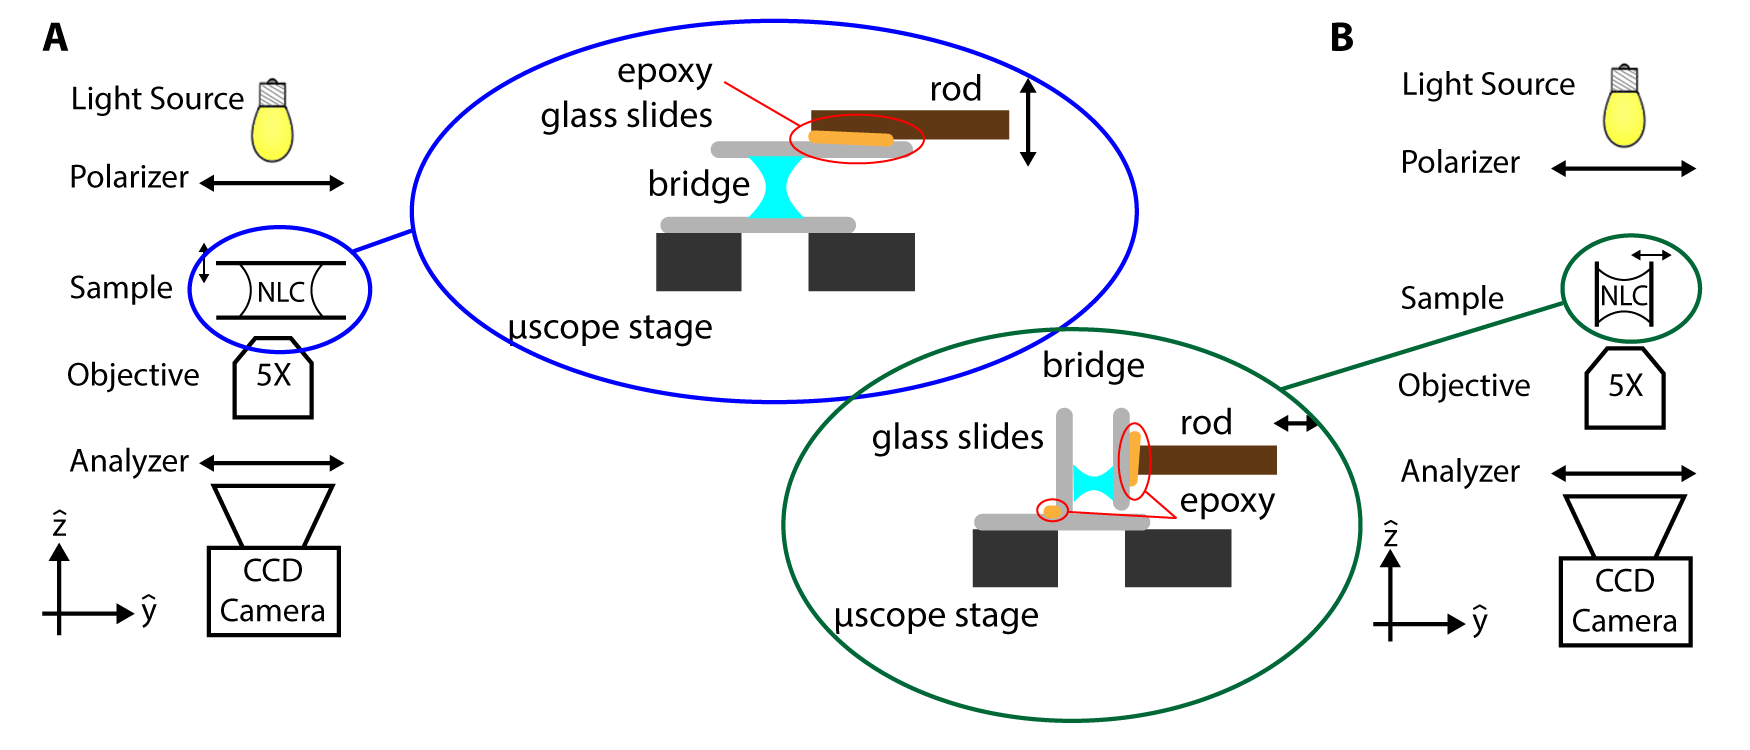
\includegraphics{figures/C5/Ch5-Figs_BuildSchematic.png}
  \caption{Experimental set-up.
  (A,B) Schematic from the side of the setup to view a bridge from the (A) top and (B) side.
  The zoomed-in portion of (A,B) highlights the setup to make and manipulate the bridge on the microscope stage.}\label{f:5-BuildSchemaic}
\end{figure}

To set up an experiment to view a bridge from the side, we place an uncoated glass slide on the microscope stage to act as a base, and then place a lecithin-coated glass slide vertically on the base and use a pair of blocks to hold it in place.
We then epoxy the lecithin-coated slide to the base, applying epoxy to only one side of the joint between the base and the lecithin-coated slide.
Once the epoxy has hardened, we remove the blocks and place the second lecithin-coated glass slide vertically on the base and against the previously-epoxied glass slide.
We then use the rod attached to the micromanipulator to hold the two vertical slides together while we epoxy the second lecithin-coated glass slide to the rod.
This protocol ensures that the two lecithin-coated glass slides are parallel to each other and perpendicular to the base.
After the epoxy hardens, we use the mircomanipulator to move the adjustable plate as far as possible from the fixed plate and place a $\sim$nl-volume drop of 5CB onto the fixed vertical plate as close to the base as we can.
Finally, we bring the adjustable plate closer to the fixed plate until it makes contact with the sessile drop and forms a capillary bridge.
The final experimental setup for a side view is depicted schematically in Figure~\ref{f:5-BuildSchemaic}(B).

As described, this procedure will yield a capillary bridge where the free-surface is in contact with air.
To make a capillary bridge with the free surface in contact with water, we first make a bridge as described above and then pipette a drop of water near the edge of the parallel plates and let capillary action fill the gap between the plates.
The water contains 8 mM SDS to enforce homeotropic anchoring.




\section{Shape of capillary bridges}
We begin by viewing the bridges from the side and characterizing their shapes.
Bridges with air as an outer medium have a waist-like shape with negative Gaussian curvature everywhere on the free surface, as shown by the bright-field image of an example bridge in Figure~\ref{f:5-ShapeContour}(A).
In contrast, as shown in the image of an example bridge in Figure~\ref{f:5-ShapeContour}(C), bridges with water and SDS as the outer medium have a barrel-like shape with positive Gaussian curvature everywhere on the free surface.
\begin{figure}
  \centering
  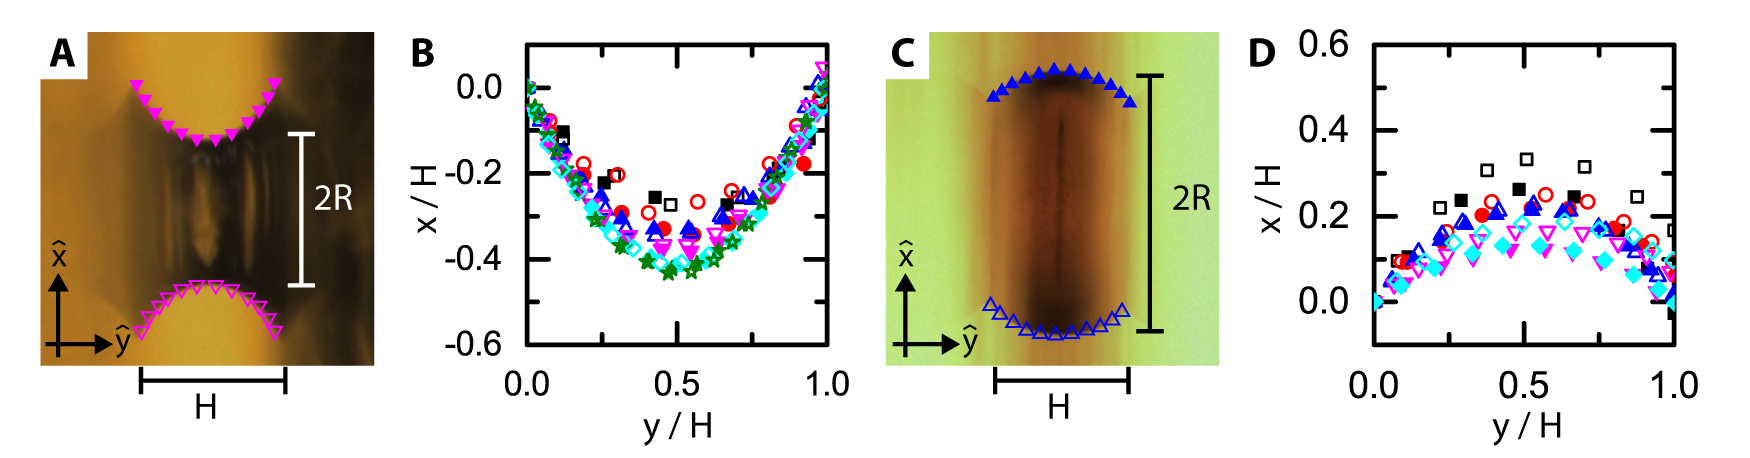
\includegraphics{figures/C5/Ch5-Figs_ShapeContour.png}
  \caption{Measuring the shape of a bridge.
  (A,C), Bright-field images from the side of a (A) waist-shaped and a (C) barrel-shaped bridge, with the effective radius $R$ and height $H$ of each bridge defined in the image.
  The waist in (A) has $R = 180$ $\upmu$m and $H = 170$ $\upmu$m, and the barrel in (C) has $R = 280$ $\upmu$m and $H = 300$ $\upmu$m.
  (B,D), Contours of the bridge shown in (A,C), respectively, at different $\Gamma = 2R/H$, where the positions have been scaled by $H$ and the (open symbols) lower contours have been reflected and shifted to line up with the (filled symbols) upper contours.
  The contours in (B) have (${\blacksquare,\, \square}$) $\Gamma = 7.3$,
   (${\color{red} \bullet,\, \circ}$) $\Gamma = 4.6$,
   (${\color{blue} \blacktriangle,\, \vartriangle}$) $\Gamma = 2.0$,
   (${\color{magenta} \blacktriangledown,\, \triangledown}$) $\Gamma = 1.0$,
   (${\color{cyan} \blacklozenge,\, \lozenge}$) $\Gamma = 0.6$, and
   (${\color{olive} \star,\, \star}$) $\Gamma = 0.4$.
  The contours in (D) have (${\blacksquare,\, \square}$) $\Gamma = 4.5$,
  ${\color{red} \bullet,\, \circ}$) $\Gamma = 3.9$,
  (${\color{blue} \blacktriangle,\, \vartriangle}$) $\Gamma = 1.9$,
  (${\color{magenta} \blacktriangledown,\, \triangledown}$) $\Gamma = 1.5$, and
  (${\color{cyan} \blacklozenge,\, \lozenge}$) $\Gamma = 1.3$.}\label{f:5-ShapeContour}
\end{figure}

\subsection{Measuring the shape}
As demonstrated on the example bridges in Figure~\ref{f:5-ShapeContour}(A,C), we record both the upper [closed symbols] and lower contours [open symbols] giving the shape of the bridge as a function of $\Gamma$, where we calculate an effective aspect ratio by taking $R$ as the radius of the circular cross-section of the bridge midway between the two confining plates and taking $H$ as the distance between the plates [see Figure~\ref{f:5-ShapeContour}(A,C)].
We then plot the contours normalized by the bridge height, with the lower contours reflected about the vertical axis, and all contours shifted so that their leftmost point corresponds to the origin, as shown in Figure~\ref{f:5-ShapeContour}(B,D) for the bridges in Figure~\ref{f:5-ShapeContour}(A,C), respectively.
For both the barrels and the waists, the respective contours all approximately have the same shape regardless of $\Gamma$ or experiment.


\subsection{Constant mean curvature surfaces}
To address the origin of the shape, we consider the relevant forces: the gravitational force $|\mathbf{F}_g| \sim \rho g R^2 H$; the surface tension force $|\mathbf{F}_{\gamma}| \sim \gamma H$; and the nematic elasticity force $|\mathbf{F}_K| \sim K$.
The surface tension, density, and Frank elastic constant of 5CB are equal, respectively, to $\gamma \approx 30$ mN/m, $\rho \approx 1$ g/mL, and $K \approx 10^{-11}$ N.
We compare these forces via two dimensionless groups: the Bond number $\rm{Bo} = \dfrac{|\mathbf{F}_g|}{|\mathbf{F}_{\gamma}|} = \dfrac{\rho g R^2}{\gamma} \sim  \mathcal{O}\left (10^{-2} \right)$, and the elasticity group,
 $\dfrac{|\mathbf{F}_{\gamma}|}{|\mathbf{F}_K|} =  \dfrac{\gamma H}{K} \sim \mathcal{O}\left (10^{5} \right )$, where we have taken $H = R = 100$ $\mu$m as representative values.
As $|\mathbf{F}_{\gamma}|$ is the dominant force, the mean curvature of the free surface of the bridge must be constant; otherwise, according to Eq.~\ref{e:3-LapPres}, there would be pressure gradients inside the bridge resulting in internal flow~\cite{RN178}.
Thus, the surface must satisfy:
\begin{equation}
  \Delta P = 2\gamma (-M) = -\gamma(\kappa_1 + \kappa_2) = \textrm{cons't},\label{e:5-ConsMeanCurv}
\end{equation}
where $\Delta P$ is the Laplace pressure, $M = {\rm tr}\{ \mathbf{L} \}/2 = (\kappa_1 + \kappa_2)/2$ is the mean curvature of the surface, and $\gamma$ is the surface tension.
In addition, note that our capillary bridges are surfaces of revolution, where a planar curve is rotated about an axis to form a surface.

We can gain further insight into the shape of our bridges by writing Eq.~\ref{e:5-ConsMeanCurv} in terms of a contour of a surface of revolution.
We can characterize such a contour in cylindrical coordinates $\{r,\varphi, z\}$, as schematically illustrated by the blue line in Figure~\ref{f:5-ShapeEnvelope}(A), with the arclength parameter, $s$, and the angle between the $r$-axis and the tangent to the contour at $s$,  $\theta$, the elevation angle.
The elevation angle naturally provides the contact angle for the surface, $\theta_0 = \theta(s=0)$, with $\theta_0$ the contact angle [blue circle, Figure~\ref{f:5-ShapeEnvelope}(A)].

For a surface of revolution in cylindrical coordinates, the principle curvatures are given by~\cite{RN35}:
\begin{equation}
  \kappa_1 = \frac{z''(r)}{(1+z'(r))^{3/2}}, \quad \kappa_2 = -\frac{z'(r)}{r\sqrt{1 + z'(r)^2}}.\label{e:5-SoRcurvatures}
\end{equation}
We can easily write ${\rm d}r/{\rm d}s$ and ${\rm d}z/{\rm d}s$ in terms of the elevation angle, ${\rm d}r/{\rm d}s = \cos \theta$ and ${\rm d}z/{\rm d}s = \sin \theta$, implying that $z'(r) = \tan \theta$.
% We can check these expressions using the relation ${\rm d}s^2 = {\rm d}r^2 + {\rm d}z^2$,
% \begin{align}
%   {\rm d}s^2 &= {\rm d}r^2 + {\rm d}z^2, \\
%   \frac{{\rm d}s^2}{{\rm d}r^2} &= 1 + z'(r)^2, \\
%   z'(r)^2 &= \sec^2 \theta - 1, \\
%   z'(r) &= \tan \theta, \label{e:4-zprime}
% \end{align}
% as desired.
Now, substituting this into Eqs.~\ref{e:5-SoRcurvatures}, we can write our principle curvatures in terms of $\theta$:
\begin{align}
  \kappa_1 = \frac{1}{R_1} &= \frac{\frac{\rm d}{{\rm d}r} \tan \theta}{(1 + \tan ^2 \theta)^{(3/2)}}, \\
           &= \frac{\frac{{\rm d}\theta}{{\rm d}r} \frac{\rm d}{{\rm d}\theta} \tan \theta}{\sec^3 \theta}, \\
           &= \frac{{\rm d}\theta}{{\rm d}s} \frac{{\rm d}s}{{\rm d}r} \cos \theta, \\
           &= \frac{{\rm d}\theta}{{\rm d}s}.\label{e:5-kappa1} \\
  \kappa_2 = \frac{1}{R_2} & = -\frac{\tan\theta}{r \sqrt{1 + \tan^2\theta}} \\
           &= -\frac{\sin \theta}{r}.\label{e:5-kappa2}
\end{align}

From Eq.~\ref{e:5-kappa1}, we can write $ds = R_1 d\theta$, which makes sense considering that $\theta(s)$ is also the angle between $\hat{z}$ and the normal to the curve at $s$; the first principle curvature describes how the surface changes in the $rz$-plane.
Similarly, from Eq.~\ref{e:5-kappa2}, we can write $R_2 = r/\sin\theta$, showing that the second radius of curvature is the distance from the contour to the z-axis along the normal to the contour.
More importantly, this shows that $R_2$ always originates on the $z$-axis for a surface of revolution.
Finally, if our bridges truly are surfaces of revolution with constant mean curvature, then the contours in Figure~\ref{f:5-ShapeContour}(B,D) must satisfy:
\begin{align}
  \frac{\textrm{d}\theta}{\textrm{d}s} &= \frac{\sin \theta}{r} - \frac{\Delta P}{\gamma},\label{e:5-ShapeSolveA} \\
  \frac{{\rm d}r}{{\rm d}s} &= \cos \theta, \\
  \frac{{\rm d}{z}}{{\rm d}s} &= \sin \theta.\label{e:5-ShapeSolveC}
\end{align}

These three equations can be solved with three initial conditions where $s = 0$.
We control the height of the bridge in our experiments, determining $z(s = 0)$.
As mentioned earlier, the contact angle is the initial condition on $\theta$, $\theta_0 = \theta(s=0)$.
Finally, since the volume is fixed in our experiments, this determines the final condition $r(s=0)$.
However, since the contours in Figure~\ref{f:5-ShapeContour}(B,D) have all been scaled by $H$ as well as all been shifted to all begin at $(0,0)$, the actual values of $z(s = 0)$ and $r(s = 0)$ do not affect the shape.
Accordingly, the difference between the contours for a waist [Figure~\ref{f:5-ShapeContour}(B)] and the contours for a barrel [Figure~\ref{f:5-ShapeContour}(D)] can only come from $\theta_0$.
Thus, the contact angle between the lecithin-coated glass slide, the outer medium, and the 5CB determines the shape of our bridges~\cite{RN178}.
\begin{figure}
  \centering
  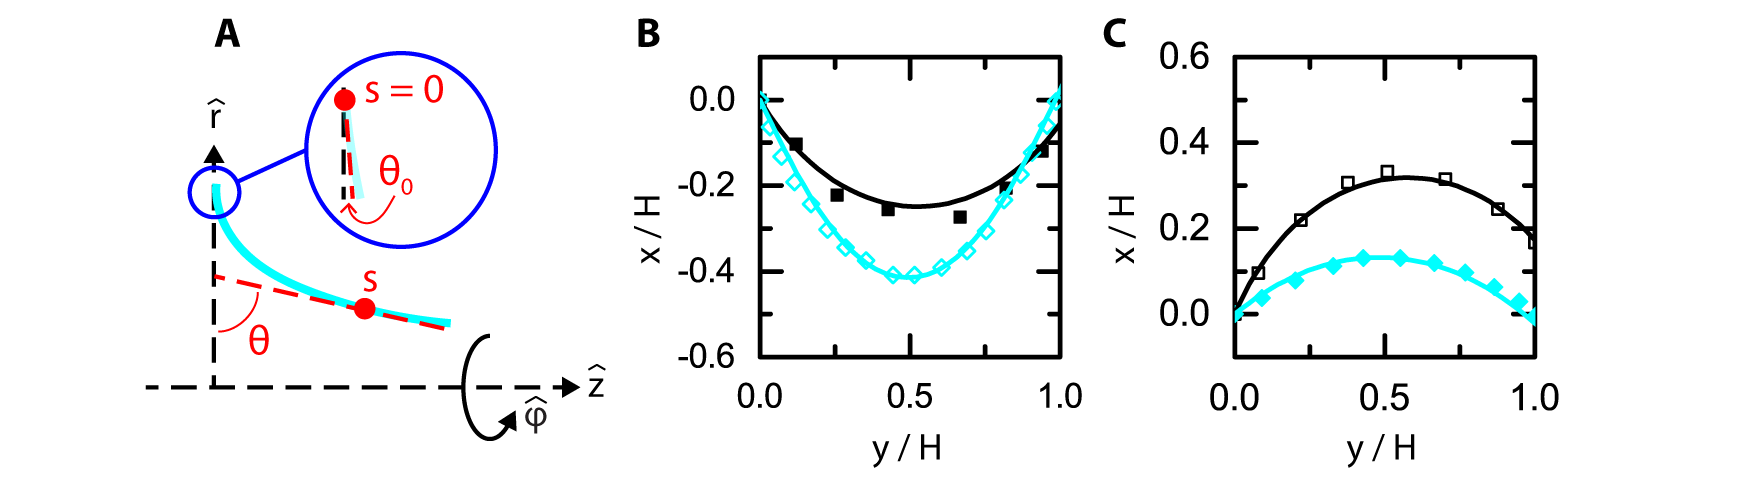
\includegraphics{figures/C5/Ch5-Figs_ShapeEnvelope.png}
  \caption{Constant mean curvature surfaces.
  (A), The elevation angle $\theta$ and arclength parameter $s$ defined for a surface of revolution in cylindrical coordinates, $\{r,\varphi, z\}$, with a contour of the surface displayed in cyan.
  $\theta$ is the angle between the tangent of the cyan curve at $s$ and $\hat{r}$.
  $\theta(s=0) = \theta_0$, the contact angle, as shown in the magnified section in the blue circle.
  (B,C), Numerically calculated contours for a constant mean curvature surface of revolution plotted on experimentally measured contours for a (B) waist and a (C) barrel.
  The numerical solutions have contact angles (B) (black line) $\theta_0^{waist} = 37^{\circ}$, (cyan line) $\theta_0^{waist} = 35^{\circ}$ and (C) (black line) $\theta_0^{barrel} = 149^{\circ}$, (cyan line) $\theta_0^{barrel} = 120^{\circ}$.
  The measured contours in (B,C) are reproduced from Figure~\ref{f:5-ShapeContour}(B,D), respectively, and form the envelope of the measured contours in Figure~\ref{f:5-ShapeContour}(B,D).}\label{f:5-ShapeEnvelope}
\end{figure}

To confirm this, we consider each bridge and numerically integrate Eqs.~\ref{e:5-ShapeSolveA}--\ref{e:5-ShapeSolveC} to produce constant-mean curvature contours that capture the observed contours in Figure~\ref{f:5-ShapeContour}.
We consider datasets in these figures representative of the spread observed, see Figure~\ref{f:5-ShapeEnvelope}(B,C).
To generate the numerical contours we start by making Eqs.~\ref{e:5-ShapeSolveA}--\ref{e:5-ShapeSolveC} dimensionless by dividing all lengths with $H$, such that $z(s = 0) = -1/2$ and $r(s = 0) = \Gamma/2$.
Note that since $\Gamma$ is measured in the middle of the two plates, $r(s = 0) = \Gamma/2$ is not accurate, but since the contours are shifted to all start at the same point, we emphasize again that $r(s = 0)$ doesn't affect the final shape.
We then numerically integrate Eqs.~\ref{e:5-ShapeSolveA}--\ref{e:5-ShapeSolveC} from $s = 0$ to $s = s_{lim}$, where $z(s = s_{lim}) = 1/2$, varying $\theta_0$ and $\Delta P$ until the numerical contours capture the experimental data, see Figure~\ref{f:5-ShapeEnvelope}(B,C).
For an ideal bridge where $r(s = 0) = r(s = s_{lim})$ and $\theta(s_{lim}) = \pi - \theta_0$ [blue contour, Figure~\ref{f:5-ShapeEnvelope}(B)], $\Delta P$ is not a free parameter but is determined by the constraints on $r(s = s_{lim})$ and $\theta(s_{lim})$.
However, the contact areas on the plates are not always equal in our experiments, making $r(s = 0) \neq r(s = s_{lim})$ [black contour, Figure~\ref{f:5-ShapeEnvelope}(C)].
Here, we vary $\Delta P$ for a given $\theta_0$ to best fit the data, changing $r(s = s_{lim})$ and $\theta(s_{lim})$.
We average the contact angles from the numerically-integrated contours for the waists and barrels to get $\theta^{waist}_0 = 36^{\circ} \pm 8^{\circ}$ and $\theta^{barrel}_0 = 127^{\circ} \pm 9^{\circ}$.
We compare the contact angles determined from our calculated contours with contact angles measured from sessile droplets with both air and water as the outer medium, finding $\theta_0^{air} = 37^{\circ} \pm 5^{\circ}$ and $\theta_0^{water} = 123^{\circ} \pm 5^{\circ}$.
This is in agreement with our data from the bridges, confirming that the contact angle is the main parameter determining the shape of our bridges.




\section{Defect structure transitions}
We view the bridge from the top to determine whether the defect is a ring or a point; examples of these situations are shown in the bright-field images of a waist-like bridge in Figure~\ref{f:5-ExpWaistTop}(A,C) and the corresponding crossed-polar images in  Figure~\ref{f:5-ExpWaistTop}(B,D).
\begin{figure}
  \centering
  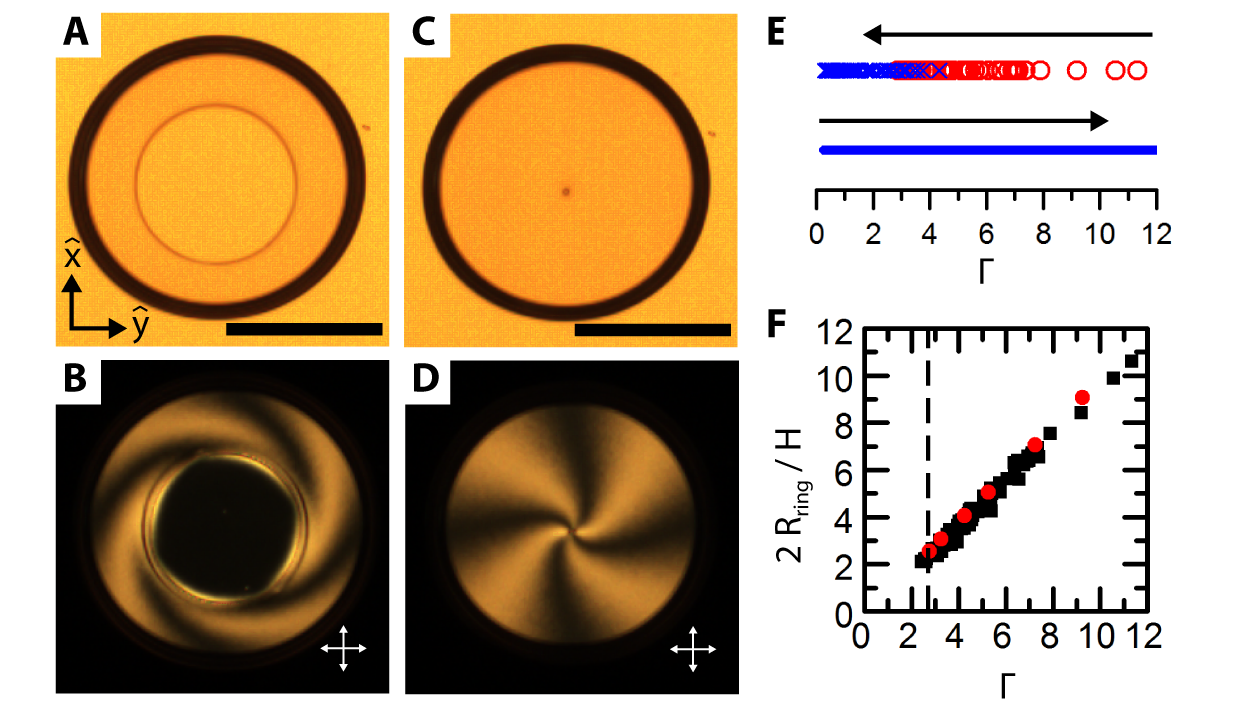
\includegraphics{figures/C5/Ch5-Figs_ExpWaistTop.png}
  \caption{Data for bright-field and optical-polarized microscopy of waist-shaped NLC bridges viewed from the top.
  (A) Example bright-field image of a waist-shaped bridge with a ring defect.
  (B) Crossed-polar image of the bridge in (A).
  (C) Example bright-field image of a waist-shaped bridge with a point defect. This is the same bridge as in (A), but with an increased distance between the plates.
  (D) Crossed-polar image of the bridge in (C).
  (E) Experimental phase diagram for the defect state, demonstrating hysteresis at the transition.
  The arrows indicate the directions in which $\Gamma$ is changed in the experiments.
  Starting at a large $\Gamma$ in the ring-defect state (${\color{red} \circ}$) and decreasing $\Gamma$ leads to a transition to a point defect (${\color{blue} \times}$) at a value of $\Gamma = 2.7 \pm 0.3$, which we obtain by averaging the result for all bridges.
  In contrast, when starting at small $\Gamma$ in a point-defect state and increasing $\Gamma$, the point-defect state persists; this is represented with a line.
  (F) The ring defect diameter in a waist-shaped bridge scaled by half the bridge height, plotted as a function of the bridge aspect ratio. A vanishing ring radius corresponds to a point defect.
  The ($\blacksquare$) are experimental measurements; the (${\color{red} \bullet}$) correspond to computations in a waist structure using the elastic constants for 5CB.\@
  Scale bars in (B,D): 250 $\upmu$m.}\label{f:5-ExpWaistTop}
\end{figure}

\subsection{Defect transitions in a waist}
We start at large $\Gamma$, where the equilibrium state has a ring defect, and determine the radius of the ring, $R_{ring}$, as we decrease $\Gamma$ by increasing $H$ in discrete steps.
At each $H$, we monitor the bridge over time to ensure that the defect state no longer changes and the system is in equilibrium.
In addition, as we decrease $\Gamma$ in each bridge, we also determine the effective aspect ratio for the defect transition, $\Gamma_c$.
Using results for 21 different bridges, we find an average $\Gamma_c = 2.7 \pm 0.3$, as shown in the upper contour in Figure~\ref{f:5-ExpWaistTop}(E), where we have plotted each observation of a stable ring defect with a (${\color{red} \circ}$) symbol and each observation of a stable point defect with a (${\color{blue} \times}$) symbol.
The ring diameter, scaled by the bridge height, varies linearly with $\Gamma$ for $\Gamma > \Gamma_c$, as indicated by the squares in Figure~\ref{f:5-ExpWaistTop}(F), where we have again plotted every measurement we have performed.
At $\Gamma_c$, the  ring becomes unstable, and collapses to a point defect, yielding the discontinuity in $R_{ring}$ shown with a dashed line in Figure~\ref{f:5-ExpWaistTop}(F), where the point defect is represented as having a vanishing $R_{ring}$.

However, when we start at $\Gamma < \Gamma_c$ in a point defect state and increase $\Gamma$, the point defect never transitions to a ring, as seen in the lower contour in Figure~\ref{f:5-ExpWaistTop}(E).
Interestingly, if for $\Gamma > \Gamma_c$, we melt the nematic phase in a bridge containing a point defect, we always recover a ring defect state when we let the bridge cool back to the nematic phase.
In contrast, when we do this for $\Gamma < \Gamma_c$, we still find a point defect when we let the bridge cool back to the nematic phase.
This suggests that the point defect is metastable for $\Gamma > \Gamma_c$.


\subsection{Defect transitions in a barrel}
% Since every barrel-shaped bridge we make initially starts as a waist, we need to make sure the defect state in the waist does not affect the final state in the barrel.
% Thus, we make our barrels both from waists with the 5CB in the nematic phase and from waists where the 5CB has been melted to the isotropic phase before adding the water and SDS mixture.
% For the barrels made with the 5CB in the isotropic phase, we also heat the water and SDS mixture before making the barrel so that the 5CB does not cool to the nematic phase before the barrel shape has been established.
As with the waist structures, we start with a large $\Gamma$ where the bridge contains a ring defect and decrease $\Gamma$ in discrete steps, measuring the ring radius at each step, as shown in the bright field images of a barrel for four values of $\Gamma$ in Figure~\ref{f:5-ExpBarrelTop}(A,C,E,G), with the associated crossed-polar images in Figure~\ref{f:5-ExpBarrelTop}(B,D,F,H).
However, over time the SDS forms micelles in the 5CB that self-assemble onto the ring defect and form visible structures [see Figure~\ref{f:5-ExpBarrelTop}(E,G)] in the NLC~\cite{RN279}.
In addition, note how the area inside the ring defect in the OPM images in in Figure~\ref{f:5-ExpBarrelTop}(B,D,F,H) becomes progressively brighter over time.
Since the SDS micelles themselves are not birefringent, this brightening implies that the micelles are affecting the director field inside the bridge.
Recall that the director field for a ring defect viewed from the top [see Figure~\ref{f:2-3DMeas}(C,D)] indicates that the area bounded by the ring should be dark when the polarizer and analyzer are crossed.
For a waist, where there is no SDS, this is always true [see Figure~\ref{f:5-ExpWaistTop}(B)].
In addition, we see that the self-assembled micelles can even stabilize non-circular ring shapes [see Figure~\ref{f:5-ExpBarrelTop}(G)] and off-center rings [see Figure~\ref{f:5-ExpBarrelRing}(B)], further indicating that the SDS can affect the director field in our bridges~\cite{RN279,RN280}.
\begin{figure}
  \centering
  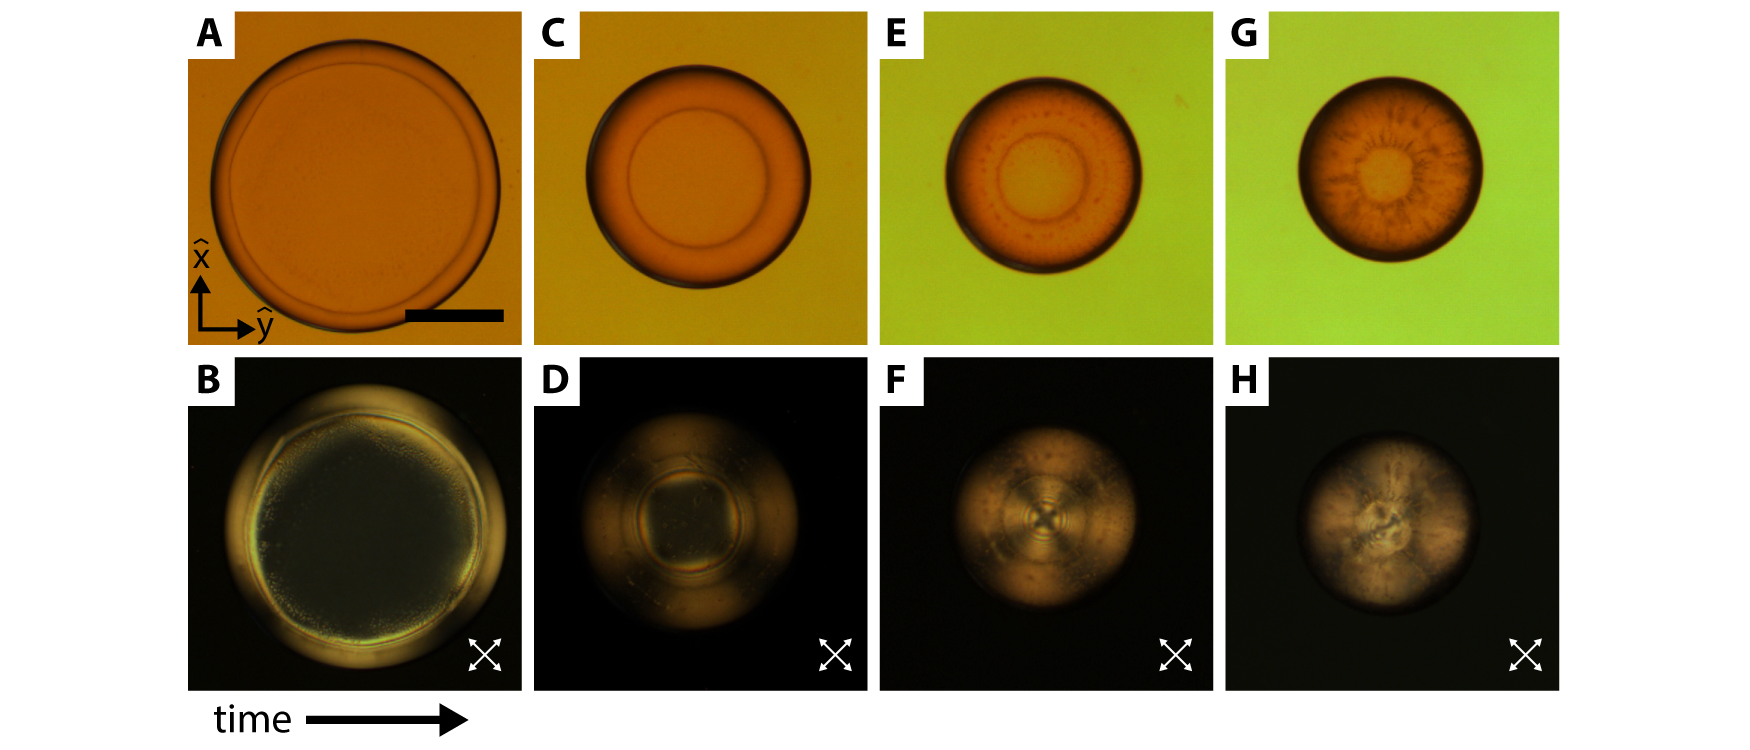
\includegraphics{figures/C5/Ch5-Figs_ExpBarrelTop.png}
  \caption{Bright-field and optical-polarized microscopy of barrel-shaped NLC bridges viewed from the top.
  (A,C,E,G), Bright-field images of a barrel-shaped bridge viewed from top with (A) $\Gamma = 5.0$, (C) $\Gamma = 2.6$, (E) $\Gamma = 1.4$, and (G) $\Gamma = 0.9$.
  Measurements were taken starting at (A) with $\Gamma = 5.0$ and decreasing $\Gamma$ in discrete steps.
  (B,D,F,H), Corresponding crossed-polar images of the bridges in (A,C,E,G), respectively.
  Note how the sodium dodecyl sulfate (SDS) used to enforce homeotropic anchoring in the barrels forms micelles and disrupts the director in the bridge over time, from the initial measurement in (A,B) to the final measurement pictured in (G,H).
  The scale bar in (A) is $250$ $\upmu$m.}\label{f:5-ExpBarrelTop}
\end{figure}

To minimize the effect of the SDS micelles, we restrict our measurements to ring defects that are circular and centered in the bridge.
We also make sure that the region within the ring in the crossed-polar images is dark, indicating that the SDS micelles have not yet significantly affected the NLC.
For example, we exclude the data in Figure~\ref{f:5-ExpBarrelTop}(E-H) and in Figure~\ref{f:5-ExpBarrelRing}(B,C).
We then plot the ring diameter scaled by the bridge height as a function of $\Gamma$ for each bridge, as seen in Figure~\ref{f:5-ExpBarrelRing}(A).
Here, the data are color coded by the measurement number for each bridge; the first measurement we make on a particular bridge is indicated by the (${\blacksquare,\, \square}$) symbols.
We then decrease $\Gamma$ and make the second measurement for that bridge, plotting the data with the (${\color{red} \blacksquare,\, \square}$) symbols.
Similarly, the third and fourth measurements on a bridge are indicated by the (${\color{blue} \blacksquare,\, \square}$) and (${\color{magenta} \blacksquare,\, \square}$) symbols, respectively.
The few magenta and blue points compared to the number of black and red points in Figure~\ref{f:5-ExpBarrelRing}(A) indicate that the effect of the micelles grows in time; we, in fact, rarely have good data to make a fourth measurement and we never have good enough data to make a fifth measurement for a given bridge.
Thus, even though we see that the scaled ring diameter varies linearly with $\Gamma$, [Figure~\ref{f:5-ExpBarrelRing}(A)], we cannot make a quantitative prediction about a ring-to-point defect transition in our barrel-shaped bridges.
This is true regardless of whether we make a barrel by adding the water + SDS to a waist with the 5CB in the nematic state [open squares, Figure~\ref{f:5-ExpBarrelRing}(A)] or with the 5CB in the isotropic state [closed squares, Figure~\ref{f:5-ExpBarrelRing}(A)].
In addition, note that the protocol used to make the barrel does not affect how the scaled ring diameter depends on $\Gamma$, indicating that the defect state in a barrel is not affected by the waist it was made from.

Even when we make barrels where the first measurement has low $\Gamma$, we do not see a clear collapse to a point defect; instead, we see a small ring defect with $0 < 2 R_{ring}/H < 0.3$, as pictured in Figure~\ref{f:5-ExpBarrelRing}(B,C) and Figure~\ref{f:5-ExpBarrelRing}(D,E) for barrels made with $\Gamma = 2.4$ and $\Gamma = 2.8$, respectively.
Since the ring in Figure~\ref{f:5-ExpBarrelRing}(B) is off-center, we exclude this data.
For the ring in Figure~\ref{f:5-ExpBarrelRing}(D), we measure $2 R_{ring}/H =0.1$, and plot the data in Figure~\ref{f:5-ExpBarrelRing}(A).
We made ten barrels with an initial $\Gamma < 5$, we excluded seven of the barrels due to SDS effects.
The remaining three barrels all have $0 < 2 R_{ring}/H < 0.3$, as plotted in Figure~\ref{f:5-ExpBarrelRing}(A).
\begin{figure}
  \centering
  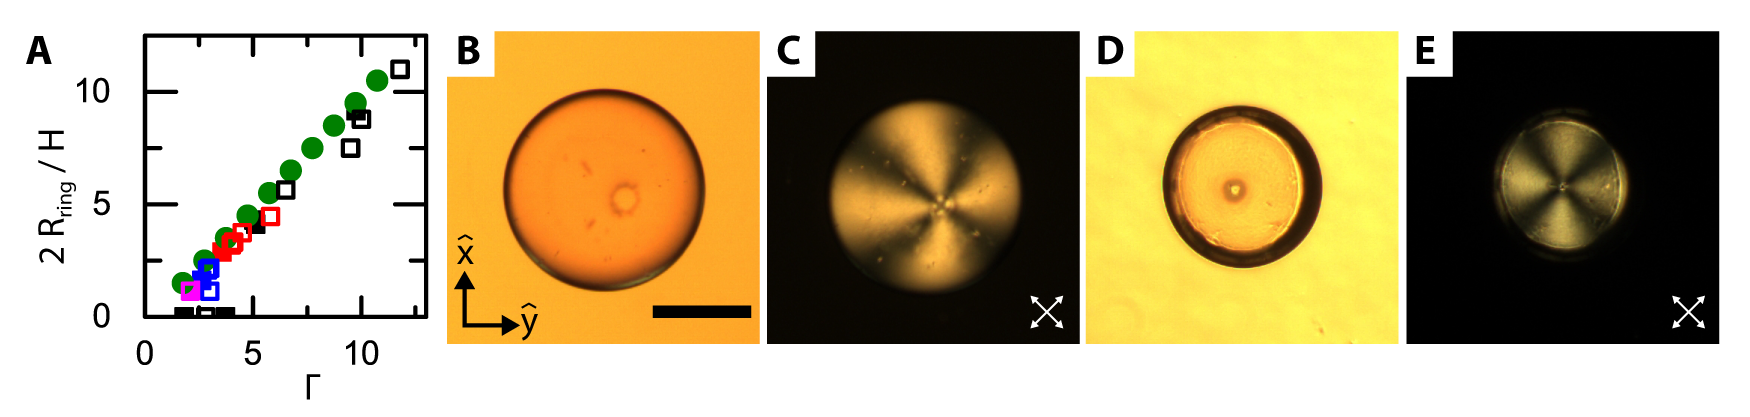
\includegraphics{figures/C5/Ch5-Figs_ExpBarrelRing.png}
  \caption{Ring defects in barrel-shaped NLC bridges viewed from the top.
  (A), The ring defect diameter in a barrel-shaped bridge scaled by height of the bridge divided by 2, plotted as a function of the bridge aspect ratio, $\Gamma$.
  The experimental points include barrels made with the 5CB in the [open squares] nematic phase and the 5CB in the [filled squares] isotropic phase.
  We label the experimental points with their measurement number, with (${\blacksquare,\, \square}$) corresponding to the first measurement, (${\color{red} \blacksquare,\, \square}$) the second measurement, (${\color{blue} \blacksquare,\, \square}$) the third measurement, and (${\color{magenta} \blacksquare,\, \square}$) the fourth measurement, where we start at a large $\Gamma$ and decrease $\Gamma$ with each subsequent measurement in a single barrel.
  The (${\color{olive} \bullet}$) correspond to computations in a barrel structure using the elastic constants for 5CB.\@
  (B--E), First measurement of a barrel with (B,C) $\Gamma = 2.4$ and (D,E) $\Gamma = 2.8$ made with the 5CB in the isotropic phase and viewed from the top just after the (B,D) bright field and (C,E) corresponding crossed-polar image indicate the director field has stopped changing.
  We exclude this bridge in (B,C) from the plot in (A) due to the presence of micelles; we cannot say if the micelles are preventing the ring from collapsing to a point defect of if the measured $2 R_{ring}/H = 0.2$ is the equilibrium state.
  The defect structure in (D,E) is a ring with $2 R_{ring}/H = 0.1$ and is plotted in (A) as such.
  The scale bar in (B) is 250 $\upmu$m.}\label{f:5-ExpBarrelRing}
\end{figure}




\section{Measuring defect conformation using fluorescence microscopy}
We return to viewing bridges from the side to determine if the defects are radial or hyperbolic.
We start by viewing the bridges with OPM and rotating the crossed polarizer and analyzer; the texture for a radial defect rotates in the same direction as the polarizer and analyzer, while the texture for a hyperbolic defect rotates with the opposite sense~\cite{RN177}.
However, due to the large curvature of the waist and barrel shapes, especially when $\Gamma$ is large, we cannot clearly distinguish the rotation of the texture.
This is demonstrated in Figure~\ref{f:5-PA_Rot} for a bridge with small $\Gamma$ [see Figure~\ref{f:5-PA_Rot}(A-C)] and a bridge with large $\Gamma$ [see Figure~\ref{f:5-PA_Rot}(D-F)].
Changing the polarizer and analyzer (P and A) orientations by 45$^{\circ}$ for the bridge with small $\Gamma$ [Figure~\ref{f:5-PA_Rot}(B,C)] produces a change in the texture, but it still does not clearly allow us to determine the brush rotation.
Rotating PA by 45$^{\circ}$ for the bridge with large $\Gamma$ [Figure~\ref{f:5-PA_Rot}(E,F)] produces an even smaller change in the texture.
As an alternative approach, we develop and use polarized epifluorescent microscopy (PFM) to see whether the defect is radial or hyperbolic.
\begin{figure}
  \centering
  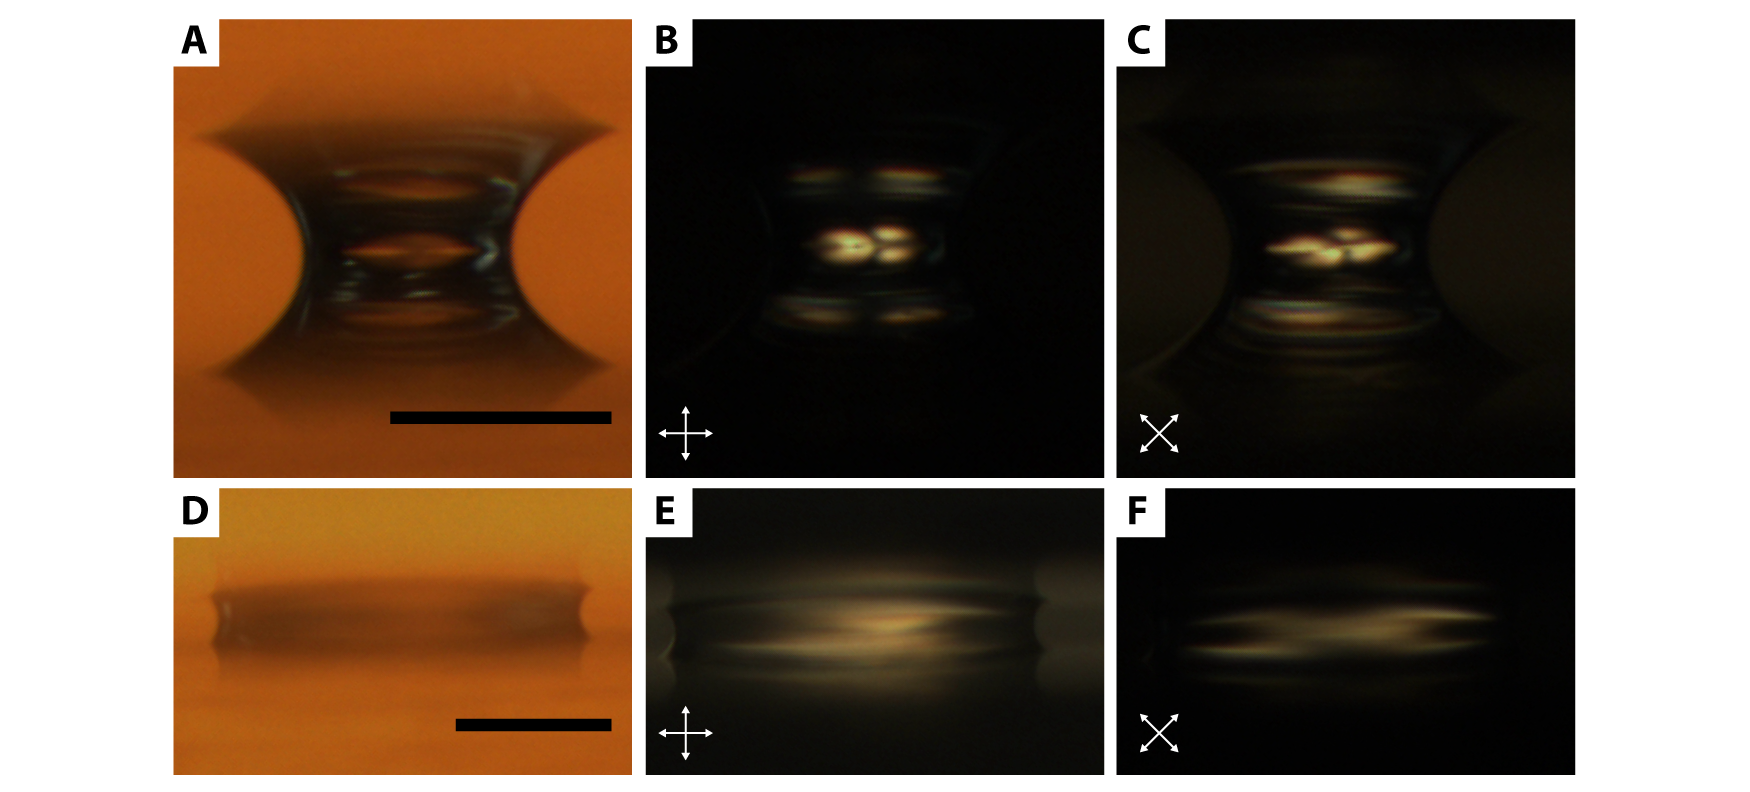
\includegraphics{figures/C5/Ch5-Figs_PA_Rot.png}
  \caption{Rotating the polarizer and analyzer for a waist-shaped bridge viewed with optical-polarized microscopy from the side.
  (A-C), A waist-shaped bridge with $\Gamma = 1.2$ viewed from the side under (A) bright field and (B,C) with crossed polarizer and analyzer (PA), where the PA orientations are specified in each image.
  (D-F), A waist-shaped bridge with $\Gamma = 6.6$ viewed from the side under (D) bright field and (E,F) with crossed PA, where the PA orientations are specified in each image.
  The scale bars in (A,D) are 250 $\upmu$m.}\label{f:5-PA_Rot}
\end{figure}

\subsection{Theoretical overview of polarized epifluorescent microscopy}
As mentioned earlier, fluorescence is an inelastic process where a material absorbs and then re-emits light.
The realization that this process consists of both absorption and emission of light is attributed to Stokes, as is the name ``fluorescence'' itself.~\cite{RN286,RN287}.
However, the understanding that fluorescent emission could be polarized came from Weigert's work with small fluorescent molecules, or fluorophores~\cite{RN285}.
Individual fluorophores absorb and emit light like dipoles, with the absorption/excitation dipole and the emission dipole not necessarily parallel to each other~\cite{RN282}.
Consequently, while an isotropic distribution of fluorophores will absorb and emit light isotropically, individual fluorophores are sensitive to the polarization of the excitation light and emit linearly polarized light along the emission dipole~\cite{RN282}.

Polarized fluorescence has proven to be an incredibly effective tool in diagnostic imaging and the medical community; for example, it is commonly used used to measure molecular or cellular mobility~\cite{RN282,RN284}.
Recently, the liquid crystal community has developed a renewed interest in polarized fluorescence, with techniques like Polarized Epifluorescent Confocal Microscopy (PCFM), enabling 3D resolution of a liquid-crystalline director~\cite{RN148,RN174}.
Here, we take inspiration from PCFM and develop Polarized Epifluorescent Microscopy (PFM), its wide-field cousin.
At its core, PFM relies on anisotropic fluorophores whose emission axis is aligned along the long axis of the fluorophore.
By introducing fluorophores in a NLC at low concentrations, the long axis of the fluorophores aligns along the nematic director without affecting the director configuration~\cite{RN148,RN174}.
Thus, the fluorescent emission of the mixed fluorophore and NLC system will be linearly polarized along the director.
If we excite the sample with unpolarized light and place an analyzer in the emitted light path, as depicted schematically in Figure~\ref{f:5-PFM_FlatCell}(A) then the emitted intensity from each point in the sample will be $\propto \cos^2{(\Phi_A-\delta)}$, where $\Phi_A$ is the orientation of the analyzer and $\delta$ is the orientation of $\mathbf{n}$ in the plane of the output image~\cite{RN174}.
However, as we use wide-field fluorescent microscopy, the recorded intensity at each point in the output image reflects an averaging of the director along the light path.
Hence, we have sacrificed the three-dimensional spatial resolution of PCFM for the simplicity of PFM.
\begin{figure}
  \centering
  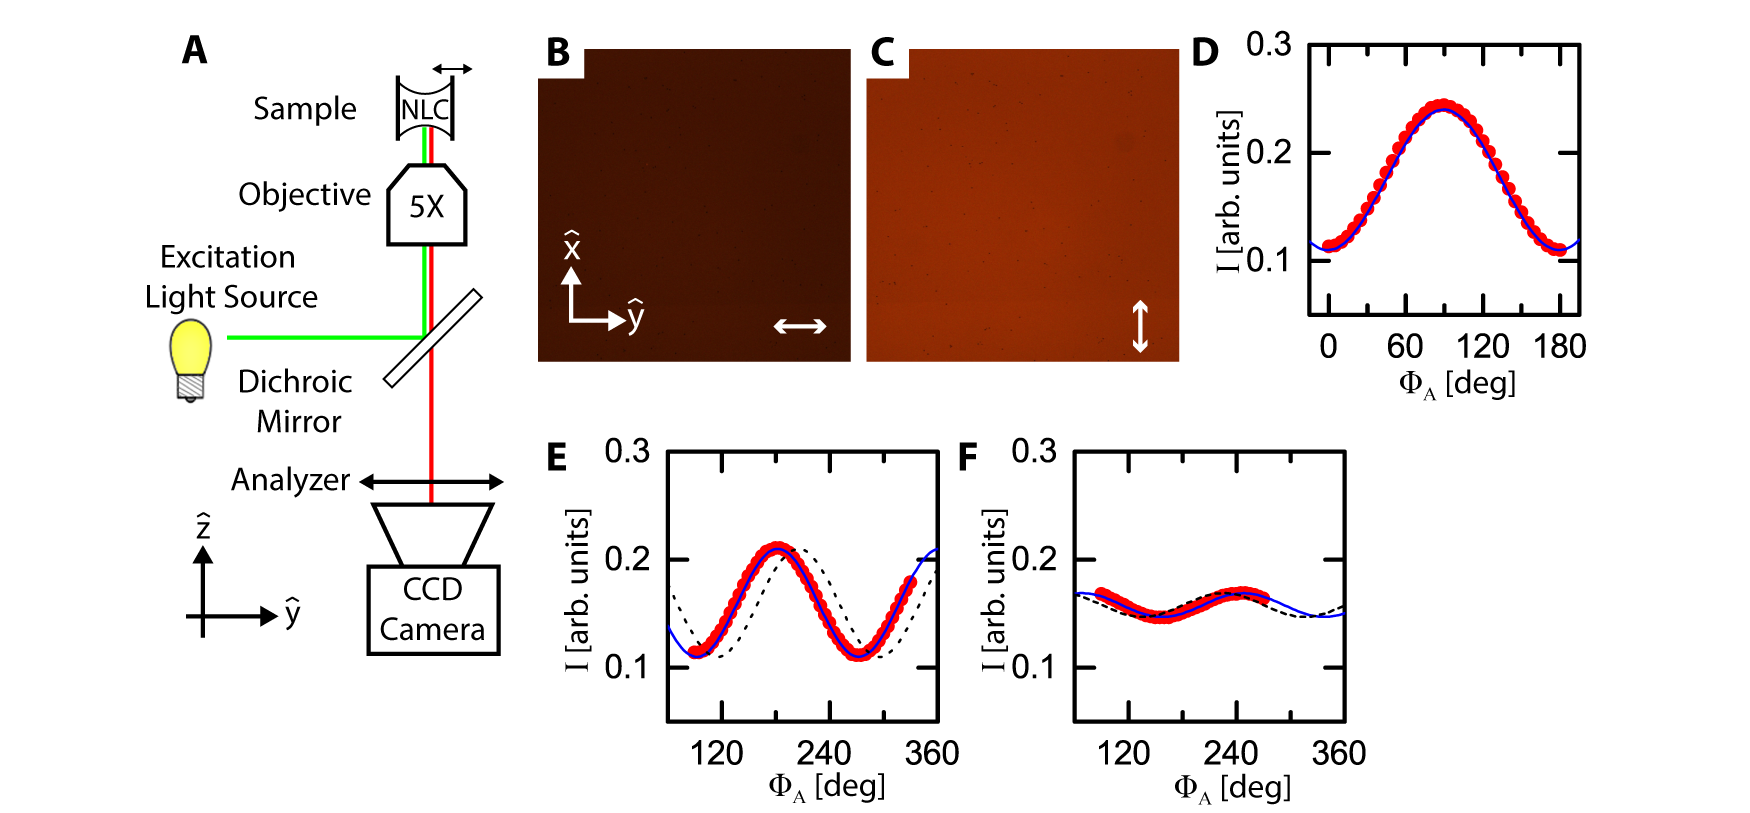
\includegraphics{figures/C5/Ch5-Figs_PFM_FlatCell.png}
  \caption{Polarized epifluorescent microscopy on a planar NLC cell filled with a mixture of 5CB and Nile Red.
  (A), Schematic from the side of the setup for polarized epifluorescent microscopy (PFM).
  (B--D), PFM (B,C) images and (D) recorded intensity as a function of $\Phi_A$ of the planar NLC cell with rubbing direction along $\hat{x}$.
  $\Phi_A$ is indicated in the images in (B,C), and is measured in (D) with respect to $\hat{y}$.
  The blue curve is a fit of the data to Eq.~\ref{e:5-IntFit}, returning $\delta' = 89^{\circ}$.
  (E,F), Recorded intensity as a function of $\Phi_A$ of the planar NLC cell with rubbing direction (E) 25$^{\circ}$ CCW from $\hat{y}$ and (F) 45$^{\circ}$ CCW from $\hat{y}$.
  The blue curves are fits of the data to Eq.~\ref{e:5-IntFit} and have $\delta' = 2^{\circ}$ and $\delta' = 67^{\circ}$, respectively.
  The black dashed lines correspond to theoretical curves for $\delta' = 25^{\circ}$ and $\delta' = 45^{\circ}$, respectively.}\label{f:5-PFM_FlatCell}
\end{figure}


\subsection{Experimental realization}
We add $0.01$ wt\% Nile red to 5CB; at this concentration, Nile red does not affect the director configuration~\cite{RN173}.
We image our sample using a standard epifluorescent setup with an analyzer in the emitted light path [Figure~\ref{f:5-PFM_FlatCell}(A)] and a short-arc lamp as our light source.
We use filter set \#20 from Zeiss, with a 534~nm~--~558~nm bandpass excitation filter, a 560~nm longpass dichroic mirror, and a 575~--~640~nm emission filter~\cite{RN288}.
For a sample, we record the output intensity $I(x,y)$ as a function of $\Phi_A$ and then fit the intensity at every pixel to the form:
\begin{equation}
    I(x,y) = A + B \cos^2{(\Phi_A-\delta'(x,y))},\label{e:5-IntFit}
\end{equation}
where $A$, $B$ and $\delta'$ are fitting parameters; $A$ and $B$ set the minimum value and range of $I$, respectively, and $\delta'$ reflects an average of the director orientation along the light path.
Using the extracted $\delta'$ values, we can then plot the associated director field for a sample.
\begin{figure}
  \centering
  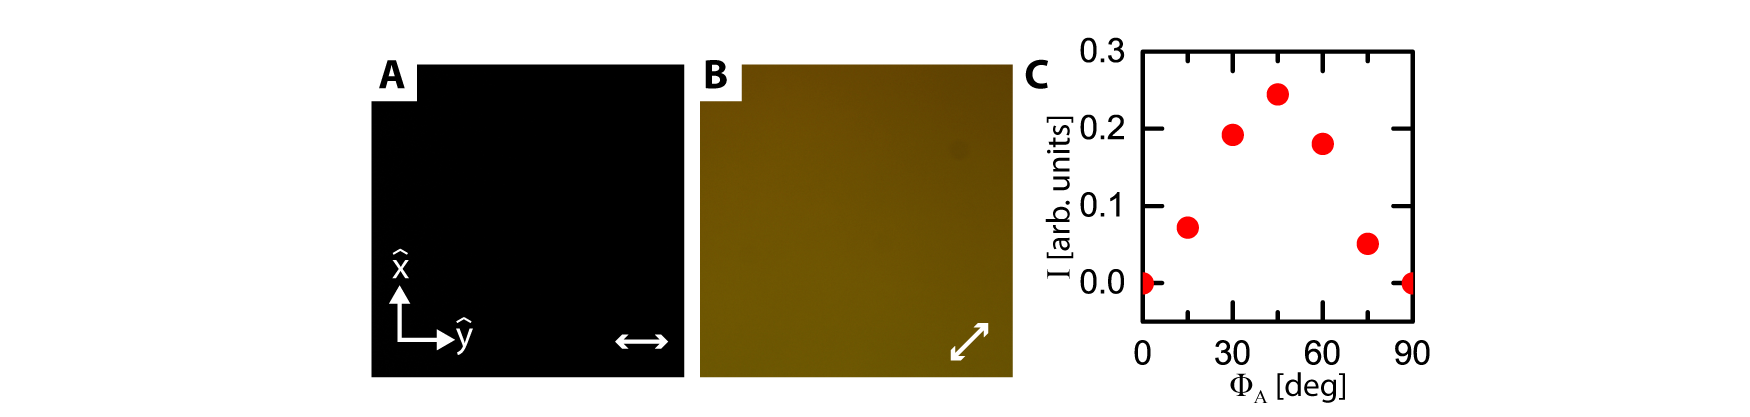
\includegraphics{figures/C5/Ch5-Figs_DichroicMirror.png}
  \caption{The dichroic mirror is birefringent.
  (A,B), Optical-polarized microscopy images with no sample, P and A crossed, and the dichroic mirror in the light path.
  $\Phi_A$ is indicated by the white arrow in the bottom-right of each image.
  (C), Transmitted intensity as a function of $\Phi_A$ for the same setup as in (A,B), with $\Phi_A$ measured CCW off of $\hat{y}$.
  The maximum at $\Phi_A = 45^{\circ}$ and minima at $\Phi_A = 0^{\circ},\, 90^{\circ}$ implies that the optic axis of the mirror is along either $\hat{x}$ or $\hat{y}$.}\label{f:5-DichroicMirror}
\end{figure}


We initially test our analysis on planar cells (INSTEC LC2-9.0) that we fill with 5CB via capillary action.
We image the cell with PFM and find that the fluorescence is much brighter when $\Phi_A$ is parallel to the rubbing direction than when $\Phi_A$ is perpendicular to the rubbing direction, as shown in Figure~\ref{f:5-PFM_FlatCell}(B,C), respectively, for a rubbing direction oriented along $\hat{x}$.
Plotting the average intensity in each image as a function of $\Phi_A$ with the (${\color{red} \bullet}$) symbols in Figure~\ref{f:5-PFM_FlatCell}(D), where $\Phi_A$ is measured off of $\hat{y}$, we see that the intensity varies as we would expect for such a rubbing direction: the intensity is a maximum when $\Phi_A = 90^{\circ}$ and a minimum when $\Phi_A = 0^{\circ}, \, 180^{\circ}$.
We fit the data in Figure~\ref{f:5-PFM_FlatCell}(D) to the expression in Eq.~\ref{e:5-IntFit} [blue curve] and find $\delta' = 89^{\circ}$, as expected.

We next change the rubbing direction to $25^{\circ}$ measured from $\hat{y}$ and plot the intensity as a function of $\Phi_A$ with the (${\color{red} \bullet}$) symbols in Figure~\ref{f:5-PFM_FlatCell}(E).
However, when we fit the data to Eq.~\ref{e:5-IntFit} [blue curve], we find $\delta' = 2^{\circ}$.
Plotting the theoretical curve for $\delta' =25^o$ [blue dashed line, Figure~\ref{f:5-PFM_FlatCell}(E)], we see that the data are shifted to the left of the expected values.
In addition, we see that the total intensity variation in the sample has decreased.
Similarly, when we do the same for a rubbing direction of $45^{\circ}$ [see Figure~\ref{f:5-PFM_FlatCell}(F)], the fit returns $\delta' = 67^{\circ}$, with the data now shifted to the right of the expected values [blue dashed line, Figure~\ref{f:5-PFM_FlatCell}(F)] and showing even less intensity variation.
We hypothesize that there is another birefringent element in the light path with its optic axis along $\hat{x}$ or $\hat{y}$; the additional retardation changes the linearly polarized light to elliptically polarized light, shifting the $I$ vs $\Phi_A$ curve and decreasing the variation in the light intensity as a function of $\Phi_A$.

We confirm this by taking OPM images with no sample and just the dichroic mirror still in the light path, as seen for P and A at $0^{\circ}$ and $90^{\circ}$ and at $45^{\circ}$ and $135^{\circ}$ in Figure~\ref{f:5-DichroicMirror}(A,B), respectively.
The bright image in Figure~\ref{f:5-DichroicMirror}(B) indicates the mirror is birefringent; plotting the transmitted intensity for crossed P and A as a function of $\Phi_A$ in Figure~\ref{f:5-DichroicMirror}(C), we see that the optic axis of the mirror is indeed along either $\hat{x}$ or $\hat{y}$.
While the mirror affects the quantitative results, we see from our experiments with the planar cell that we can still distinguish between different rubbing directions.
Finally, we also melt the 5CB in the cell to the isotropic to ensure that there is no appreciable intensity variation with changing $\Phi_A$, as shown by the relatively flat transmitted intensity curve in Figure~\ref{f:5-PFM_FlatCell}(J).
With the 5CB in the isotropic, we measure the range in the intensity variation as a function of $\Phi_A$ to be 6\% of the mean intensity.
We compare this to the cell with the rubbing direction along $45^{\circ}$, where our intensity variation with the 5CB in the nematic phase is the smallest, and find that the range in $I$ is 25\% of the mean.
This indicates that the intensity variation is due to the 5CB and not to some property of the cell.
\begin{figure}
  
\includegraphics{figures/C5/Ch5-Figs_IsotropicPlanar.png}
  \caption{Recorded intensity as a function of $\Phi_A$ of a planar NLC cell filled with 5CB and melted to the isotropic.
  The rubbing direction is along $90^o$ and the range in $I$ is 6\% of the mean.}\label{f:5-IsotropicPlanar}
\end{figure}


\subsection{Validation in spherical droplets and cylindrical capillaries}
We now turn to validating PFM using objects with a spatially varying director field.
We start by considering spherical droplets of the Nile red-doped 5CB in water, with 8 mM SDS in the water to enforce homeotropic anchoring, shown in the bright-field image in Figure~\ref{f:5-PFM_Spheres}(A).
We rotate the crossed P and A, as seen in Figure~\ref{f:5-PFM_Spheres}(B,C) for two different P and A orientations, and confirm that the droplets have the classic radial configuration~\cite{RN177}, with a single radial hedgehog at the center of each droplet.

Importantly, we also notice that when rotating the analyzer the entire image appears to translate along a circular trajectory.
Superimposing images of the spherical droplets with $\Phi_A = 0$ and $\Phi_A = \pi$ in Figure~\ref{f:5-PFM_Spheres}(D), we see that the images have been displaced.
This displacement comes from the analyzer; it has a wedge angle to prevent specular reflections from affecting the final image quality,.
However, this also serves to translate the image by $\Delta \rho$ along the orientation of the wedge angle, $\Phi_W$, as illustrated schematically in Figure~\ref{f:5-AnalyzerShift}(A).
Thus, rotating the analyzer by $\pi$ translates the image in a semicircle with radius $\Delta \rho$ [see Figure~\ref{f:5-AnalyzerShift}(B)].
This means that to properly consider $\delta'(x,y)$ as a function of $\Phi_A$, we have to correct this displacement so that $I(x,y)$ comes from the same $\delta'(x,y)$ for all $\Phi_A$.
\begin{figure}
  \centering
  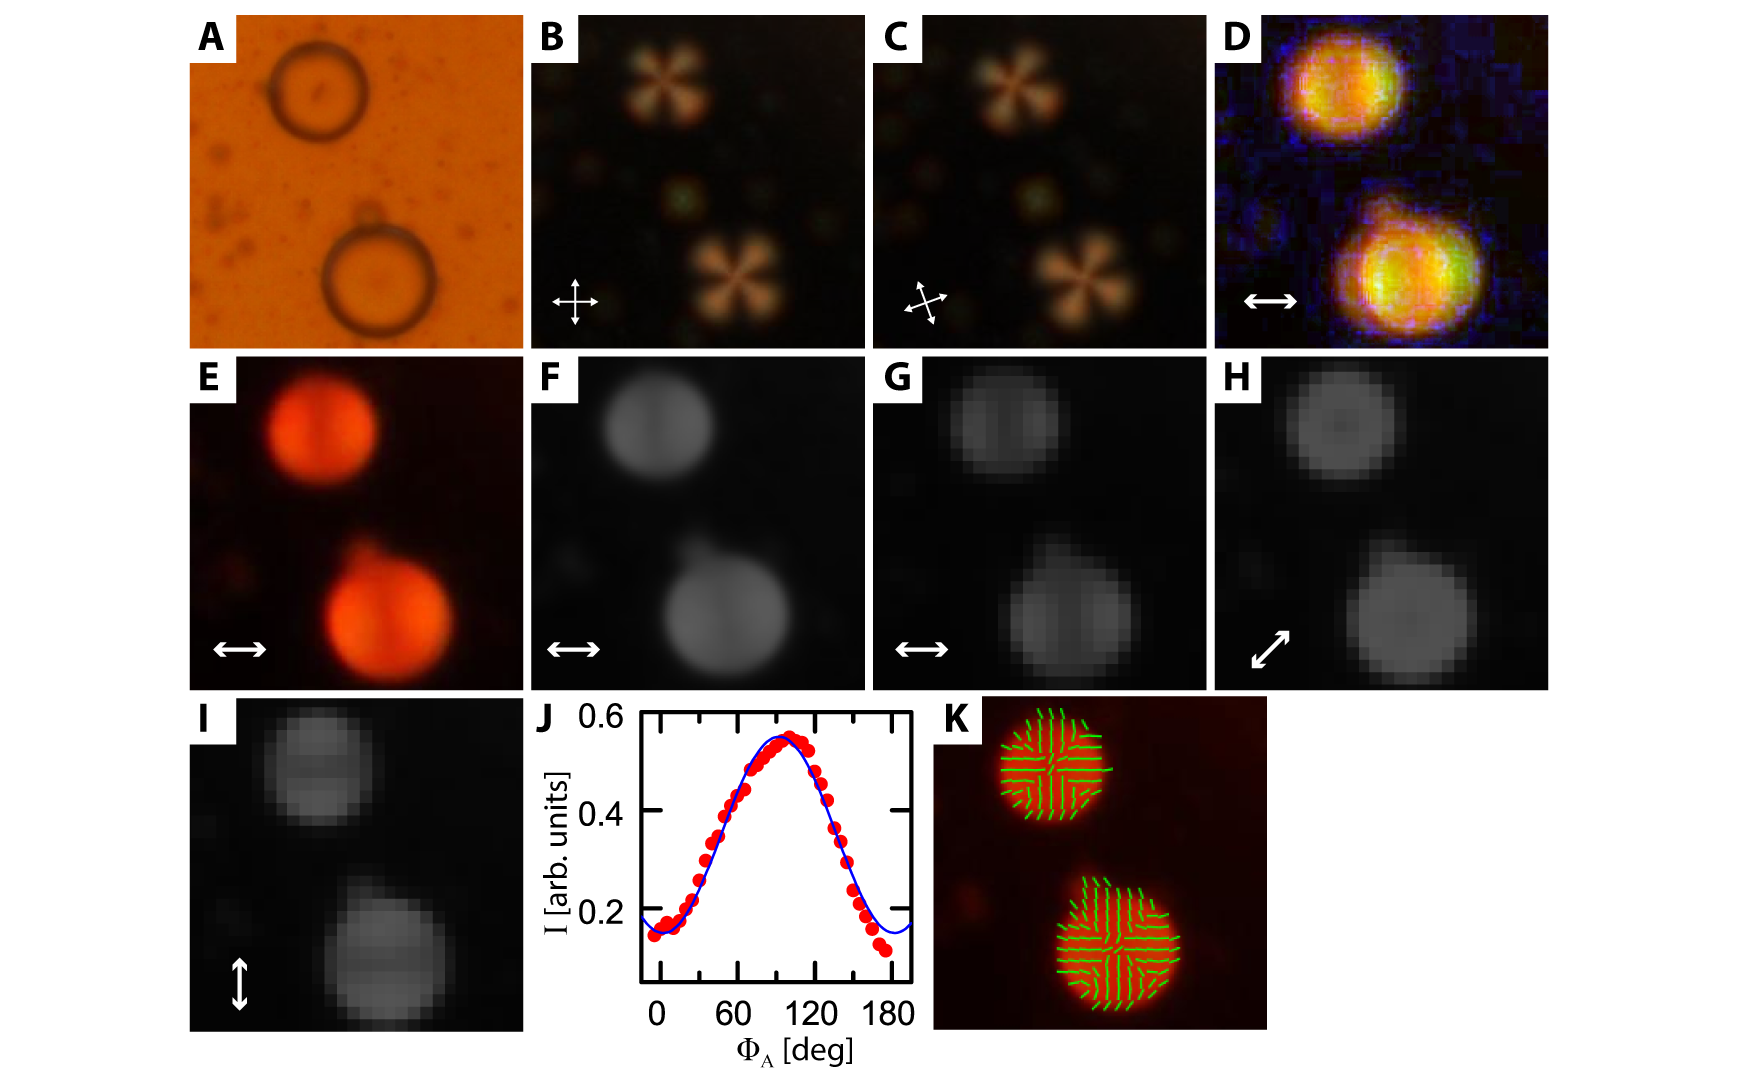
\includegraphics{figures/C5/Ch5-Figs_PFM_Spheres.png}
  \caption{PFM analysis for radial droplets.
  (A), Bright field image of radial droplets made from a mixture of 5CB and Nile red dispersed in water and 8 mM SDS.
  (B,C), Corresponding crossed-polar images of the droplets in (A) with the P and A orientation indicted in each image.
  The texture rotates with P and A, indicating the hedgehog in each droplet is radial.
  (D), Superposition of two PFM images of the droplets in (A), where the images have the same $\Phi_A$ but opposite analyzer wedge-angle orientations. Note how the two images are displaced due to the effect of the analyzer wedge-angle, making the superposition blurry.
  (E), Superposition of the same images in (D) after shifting each image to correct for the displacement due to the analyzer wedge-angle. Here, the two droplets are clear and the superposition is no longer blurry.
  The analyzer angle in (D,E) is indicated schematically.
  (F), Grayscale intensity of a PFM image of the droplets in (A) after blurring with a square Gaussian filter with side length 7 px.
  The analyzer orientation is indicated schematically.
  (G-I), Downsampled PFM images after blurring, with the analyzer angle in each image indicated schematically.
  (J), PFM intensity as a function of $\Phi_A$ from the highlighted pixel in (G-I).
  The blue curve is a fit to Eq~\ref{e:5-IntFit}, returning $\delta' = 88^{\circ}$.
  (K), The $\delta'$ from a PFM analysis of every pixel in (G-I) plotted on top of an epifluorescent image of the droplets.
  The droplets are clearly radial, matching our observations in (B,C).
  The scale bar in (A) is 25 $\upmu$m.}\label{f:5-PFM_Spheres}
\end{figure}

We accomplish this by translating all the images along their respective $\Phi_W$ by a fixed magnitude $\Delta \rho$, removing the effect of the displacement due to the analyzer wedge angle for each image.
Since $\Phi_W \in [0,\pi]$ while $\Phi_A \in [0, 2 \pi]$, we use $\Phi_A$ to determine $\Phi_W$ up to a factor of $\pi$ in each set of images; we translate an entire set by $\Delta \rho$ along both $\Phi_W = \Phi_A$ and along $\Phi_W = \Phi_A + \pi$ and keep the set where the displacement has been removed.
Note that in our microscope, $\Phi_A$ and $\Phi_W$ also differ by $30^{\circ}$ [see Figure~\ref{f:5-AnalyzerShift}(B)].
Our standard microscope setup with a $5\times$ objective and a $0.5 \times$ adapter in front of the camera (The Imaging Source, DMK 41BU02) has $\Delta \rho = 6$ px.

Now superimposing the corrected versions of the images used in Figure~\ref{f:5-PFM_Spheres}(D), we see in Figure~\ref{f:5-PFM_Spheres}(E) that the displacement between the two images has disappeared.
While in principle we could consider $\delta'(x,y)$ for every pixel, that is more information than we need and is susceptible to pixel-level noise.
Instead, we blur each image with a mean filter to both remove noise and locally average the $\delta'$, and then downsample each image to reduce the number of fits we need to perform.
We illustrate this with the example PFM images in Figure~\ref{f:5-PFM_Spheres}(F-I), where the analyzer angle is indicated in each image.
The original image is convolved with a mean filter of side length 7 px, yielding the blurred image in Figure~\ref{f:5-PFM_Spheres}(F) and then downsampled by a factor of 7, as displayed in Figure~\ref{f:5-PFM_Spheres}(G).
Here, we focus on the highlighted pixel in the downsampled images in Figure~\ref{f:5-PFM_Spheres}(G-I) and plot the intensity in Figure~\ref{f:5-PFM_Spheres}(J).
A fit of Eq~\ref{e:5-IntFit} to the data in Figure~\ref{f:5-PFM_Spheres}(J) yields $\delta' = 88^{\circ}$.
We do this for every pixel in the downsampled images and plot $\delta'(x,y)$ on top of the epifluorescent image in Figure~\ref{f:5-PFM_Spheres}(K).
Indeed, we see that we qualitatively capture the radial texture.
Note that we are unable to distinguish the actual point singularity due to the wide-field nature of our technique and the influence of the mirror; however, we clearly detect the presence of a radial defect in each droplet.
\begin{figure}
  \centering
  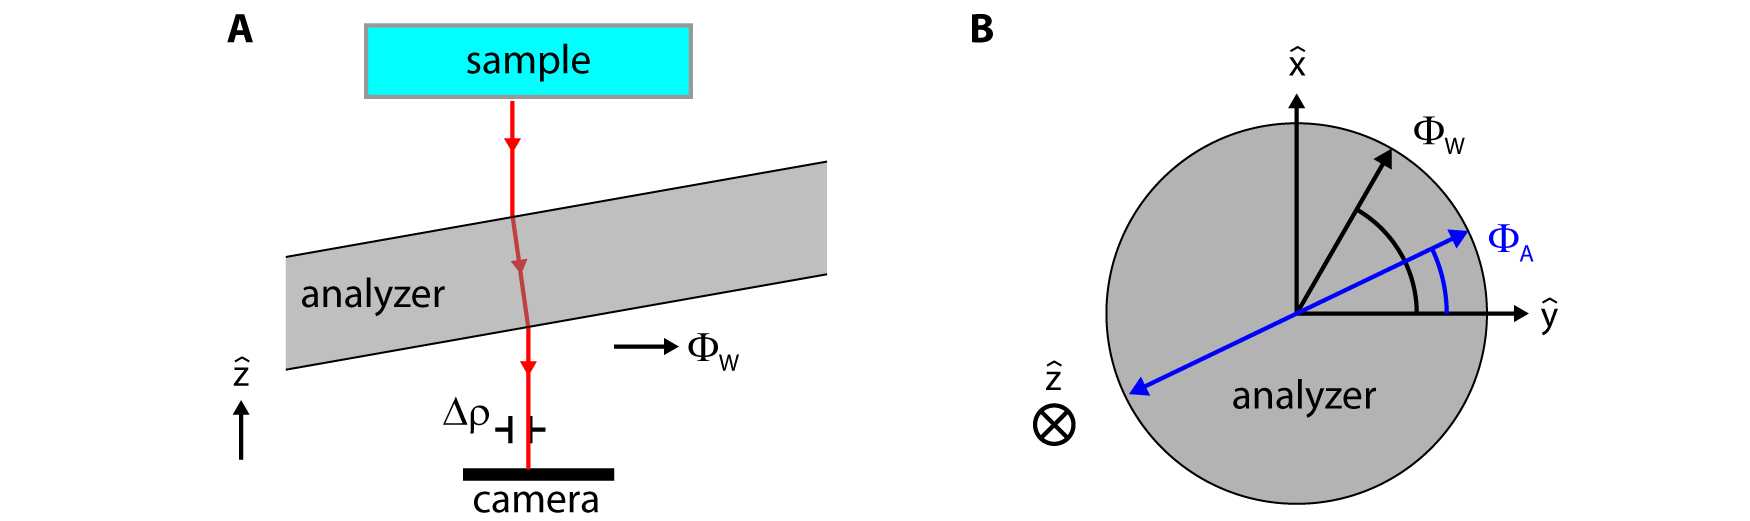
\includegraphics{figures/C5/Ch5-Figs_AnalyzerShift.png}
  \caption{The analyzer shifts the image.
  (A), Schematic from the side showing how the wedge angle of the analyzer causes light from the sample to be translated by $\Delta\rho$ in the direction of the wedge, $\Phi_W$.
  (B), The analyzer pass axis and the wedge angle are not parallel to each other.
  Rotating the analyzer by $\pi$ will translate the image on the camera along a semicircle with radius $\Delta\rho$.
  Since $\Phi_A \in [0, \pi]$ while $\Phi_W \in [0, 2 \pi]$, knowing $\Phi_A$ alone is not enough to know which direction the output image has been translated.}\label{f:5-AnalyzerShift}
\end{figure}

We next consider a cylindrical capillary filled with Nile red-doped 5CB.\@
The capillary has a 600 $\upmu$m inner diameter and is coated with lecithin to enforce homeotropic anchoring; it has a escaped-radial configuration with a point defect separating regions that escape in opposite directions~\cite{RN179}, as seen in the crossed-polar images in Figure~\ref{f:5-PFM_Capillary}(A).
We confirm that the defect is a radial point by rotating the crossed polarizer and analyzer and observing that the brushes follow the sense of rotation.
We then image the capillary using PFM, where we have shifted, blurred, and downsampled the images as with the radial droplets in Figure~\ref{f:5-PFM_Spheres}, and plot the output $\delta'$ on top of a bright-field image of the capillary in Figure~\ref{f:5-PFM_Capillary}(B).

As with the droplets, we see that we qualitatively capture the expected escaped-radial texture; we capture the radial character of the defect between the two escaped domains, but we do not resolve the singularity itself in our output.
Since the escaped-radial director field for 5CB has been analytically solved~\cite{RN289,RN290}, with $\mathbf{n}(r,\varphi,z) = \left \{ \sin(\Omega), 0, \cos(\Omega)   \right \}$, where $\Omega = 2 \arctan(r/R) $, with $R$ the capillary radius in cylindrical coordinates and $\hat{z}$ along the capillary axis, we can compare the theoretical $\Omega$ with our measured $\delta'$, as plotted in Figure~\ref{f:5-PFM_Capillary}(C).
% Again, we see deviation, with our results biased towards $0^{\circ}$ and $90^{\circ}$.
Even though there are quantitative differences, we can clearly see from both the plot of $\delta'$ vs $x/R$ [Figure~\ref{f:5-PFM_Capillary}(B)] and the plotted $\delta'$ fields [Figure~\ref{f:5-PFM_Capillary}(C)] that we capture the different escape directions and thus can also resolve the radial character of defect between them.
\begin{figure}
  \centering
  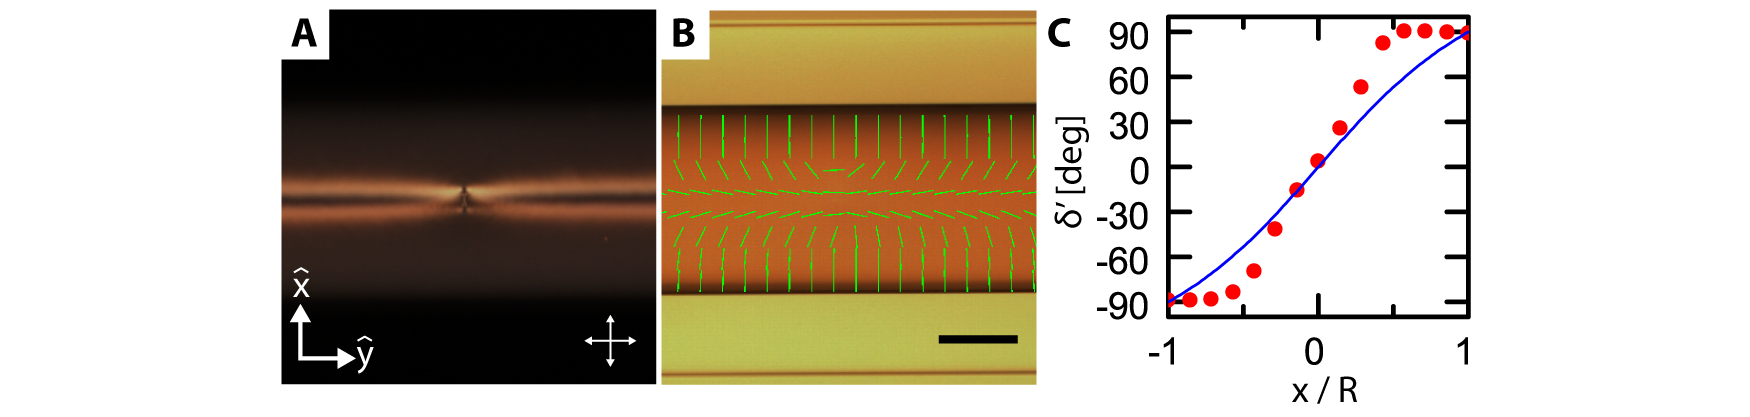
\includegraphics{figures/C5/Ch5-Figs_PFM_Capillary.png}
  \caption{PFM in an escaped-radial capillary.
  (A), Crossed-polar image of a capillary filled with the Nile Red-Doped 5CB under homeotropic anchoring.
  (B), Bright-field image of the capillary in (A), with the director orientation from the PFM analysis plotted on top of the associated bright-field image.
  (C), $\delta'$ plotted versus the position across the capillary for the column indicated by the red arrow in (B).
  The blue curve is $2 \arctan (x/R)$, the theoretical director angles for an escaped-radial configuration in the one-constant approximation.
  Using the 5CB value of $K_{11}/K_{33} = 0.74$ would only slightly change the blue curve.
  The scale bar in (B) is 250 $\upmu$m.}\label{f:5-PFM_Capillary}
\end{figure}

\subsection{Radial and hyperbolic defects in waists and barrels}
We now use PFM on our waist-shaped bridges to determine if the defect is radial or hyperbolic.
Since the output of PFM is biased due to the dichroic mirror, we orient the bridges with the plates along $45^{\circ}$, as seen in the bright-field image of a bridge in Figure~\ref{f:5-PFM_Bridge}(A), such that PFM will best distinguish the differences between a radial and a hyperbolic defect.
We start with the waist-shaped bridges; for each bridge we perform a PFM analysis and plot the $\delta'$ on top of an epifluorescent image, as shown for an example bridge with large $\Gamma$ in Figure~\ref{f:5-PFM_Bridge}(A,B) and an example bridge with small $\Gamma$ in Figure~\ref{f:5-PFM_Bridge}(C,D).
For both examples, we see that the defect structure is hyperbolic.
We do this for waist-shaped bridges spanning $\Gamma \ll \Gamma_c$ to $\Gamma \gg \Gamma_c$, and find that the defect is always hyperbolic, implying that our waist-shaped bridges undergo transitions from a hyperbolic ring to a hyperbolic point as $\Gamma$ decreases.
\begin{figure}
  \centering
  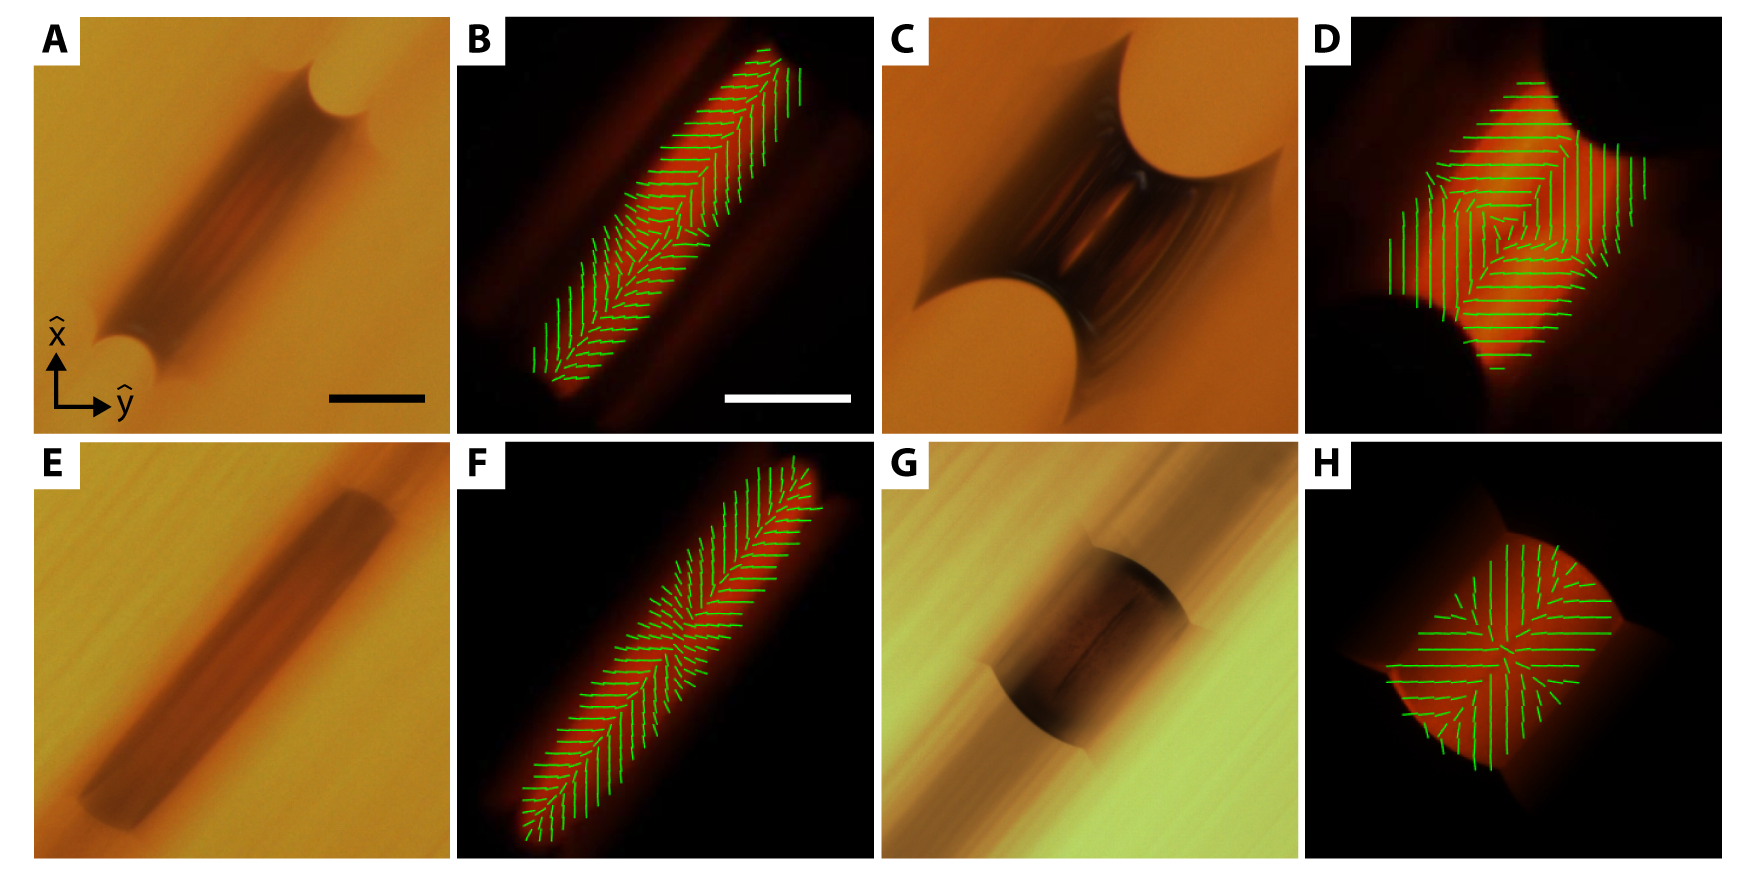
\includegraphics{figures/C5/Ch5-Figs_PFM_Bridge.png}
  \caption{(A-D), PFM analysis on waist-shaped bridges with (A,B) $\Gamma = 4.0$ and (C,D) $\Gamma = 0.8$.
  The $\delta'$ are plotted on the epifluorescent images in (B,D) with the associated bright-field images in (A,C).
  (E-H), PFM analysis on barrel-shaped bridges with (E,F) $\Gamma = 6.6$ and (G,H) $\Gamma = 1.5$.
 The $\delta'$ are plotted on the epifluorescent images in (F,H) with the associated bright-field images in (E,G).
 The scale bars in (A,B) are 250 $\upmu$m, with the scale for all the (A,C,E,G) bright field images and all the (B,D,F,H) PFM images the same.}\label{f:5-PFM_Bridge}
\end{figure}

We now turn to barrel-shaped bridges, where we add the water and SDS mixture when the 5CB is in the isotropic phase, and we consider barrels made with both a large and a small initial $\Gamma$.
As demonstrated in the plots of $\delta'$ on top of epifluorescent images of two example barrels with different $\Gamma$ in Figure~\ref{f:5-PFM_Bridge}(E-H), the barrel-shaped bridges at all measured $\Gamma$ have radial defects.
Thus, we see that the shape of the bridge, driven by the contact angle, determines if the defect is radial or hyperbolic.
This makes sense intuitively as the homeotropic boundary conditions cause the boundary to act as a level surface for the director.

Due to the ability of shape to bias the defect structure, the cylindrical bridge becomes an interestingly peculiar case, as the shape is neither a waist nor a barrel.
While accomplishing this experimentally in our system would be technically difficult due to the requirement of maintaining $\Theta_0 = 90^{\circ}$, we can turn to numerical calculations to explore this scenario.




\section{Comparison with numerical calculations: stable and metastable states}
We compare our results with numerical calculations performed by Shengnan Huang and Paul Goldbart.
These assume the problem is completely 2D; for a bridge parameterized in cylindrical coordinates, $\mathbf{n}(r,\varphi,z) = \left \{ \sin(\Omega), 0, \cos(\Omega)   \right \}$, where $\Omega = f(r,z)$ only.
We then minimize the free-energy using a version of the finite difference method laid out in Ref.~\cite{RN144}, modified as follows.
Although the free energy in the algorithm presented there depends on the cut-off length of the defect core, the equilibrium defect configuration is independent of this length scale provided it is reasonably small.
We modify the algorithm to treat the small region containing the defect separately from the remainder of the computation volume, such that the calculated free energy converges as the mesh size grows~\cite{RN199,RN200,RN201}.

A cylindrical bridge is considered first.
For the 5CB values of $K_{11}/K_{33} = 0.74$, a bridge should undergo a defect transition between a radial ring and a hyperbolic point, as highlighted by the dashed line in the phase diagram in Figure~\ref{f:5-Calcs}(A).
This result is consistent with prior computational modeling~\cite{RN144}, and highlights the peculiarity of the cylindrical case.
However, the calculations find ring-to-point defect transitions at aspect ratios that are significantly smaller than previously reported~\cite{RN144}.
In addition, in contrast to prior modeling, the calculations show no transition to a radial point structure~\cite{RN144}; only the hyperbolic point structure is stable [Figure~\ref{f:5-Calcs}(A)].
Instead, the numerical calculations predict that the radius of the radial ring should vary linearly with $\Gamma$ for the entire range of $\Gamma$ explored.
\begin{figure}
  \centering
  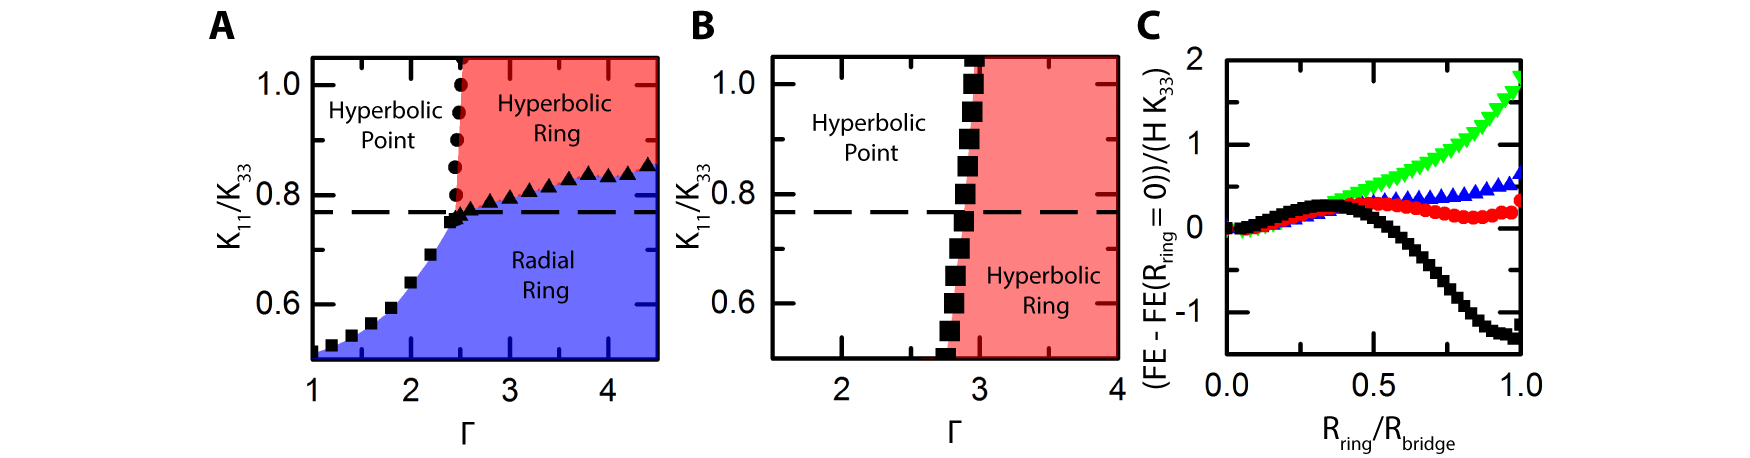
\includegraphics{figures/C5/Ch5-Figs_Calcs.png}
  \caption{Results from the computational modeling of a nematic in a capillary bridge.
  (A), Phase diagram of the defect structure in a cylinder as a function of aspect ratio $\Gamma$ and the ratio, $K_{11}/K_{33}$, of the splay and bend elastic constants.
  (B), Phase diagram of the defect structure in a waist-shaped bridge as a function of $\Gamma$ and $K_{11}/K_{33}$.
  In (A,B), the minimum-energy state is indicated in each region, and the dashed line corresponds to $K_{11} / K_{33}$ for 5CB.\@
  (C,D), Free energy of a director configuration in a waist-shaped bridge relative to the free energy in the presence of the point defect and normalized by $H K_{33}$, shown as a function of scaled ring radius $R_{ring}/R_{bridge}$.
  The curves correspond to (${\blacksquare}$) $\Gamma = 3.5$, (${\color{red} \bullet}$) $\Gamma = 2.8$, (${\color{blue} \blacktriangle}$) $\Gamma = 2.5$, and (${\color{green} \blacktriangledown}$) $\Gamma = 2.0$.}\label{f:5-Calcs}
\end{figure}

Next, the shape of the boundaries in the numerical calculations are changed.
Consistent with our experiments, it is found that the radial defects in the phase diagram for a waist-shaped bridge disappear for all values of $K_{11}/K_{33}$ used, as shown in Figure~\ref{f:5-Calcs}(B).
Furthermore, the ring defect radius in Figure~\ref{f:5-ExpWaistTop}(F) predicted by the calculations (${\color{red} \bullet}$) for a waist-like shape agrees very well with our experimental data ($\blacksquare$).
In addition, the hyperbolic-ring to hyperbolic-point transition is found to happen at $\Gamma_c = 2.7$ for $K_{11}/K_{33} = 0.74$ [dashed line, Figure~\ref{f:5-Calcs}(B)], in agreement with our experimental measurement of $\Gamma_c = 2.7 \pm 0.3$ for decreasing $\Gamma$.

To investigate the hysteresis in our experimental hyperbolic ring to hyperbolic point transition, the energy landscape of a waist-shaped nematic bridge as a function of ring radius is calculated.
Results for two bridges having $\Gamma > \Gamma_c$ and for two bridges having $\Gamma < \Gamma_c$ are shown in Figure~\ref{f:5-Calcs}(C,D), where we have taken $K_{11}/K_{33} = 0.74$; recall that the point defect is represented by the free energy for a vanishing ring radius.
As the free energy exhibits a local minimum at $R_{ring} = 0$ [Figure~\ref{f:5-Calcs}(D)], we indeed see that the point defect is metastable for $\Gamma > \Gamma_c$, consistent with our interpretation of the experimental results.
In addition, given a representative bridge height of $H = 100$ $\upmu$m and $K_{33} \approx 10^{-11}$ N, we find that the height of the barrier is always $\mathcal{O} \left ( 10^{4} \right )$ k$_\textrm{B}$T, implying that a point defect will not spontaneously transform into a ring defect over the duration of our experiments, also consistent with our experimental observations.
For $\Gamma < \Gamma_c$, this metastability disappears, and the hyperbolic point defect is the only stable defect state.

Turning to barrel-shaped bridges, the calculations show that all hyperbolic defects disappear from the phase diagram, leaving the radial ring as the only equilibrium state for the range of $\Gamma$ and $K_{11/K_{33}}$ explored.
This confirms that the shape of the free surface determines if the enclosed defect is radial or hyperbolic.
Barrel-like shapes with positive Gaussian curvature favor radial defects and waist-like shapes with negative Gaussian curvature favor hyperbolic defects.
We also see that the ring radius in Figure~\ref{f:5-ExpBarrelRing}(A) predicted by the calculations (${\color{olive} \bullet}$) in a barrel-shaped bridge also agrees with our experimental results (squares), despite the influence of the SDS micelles in the experiments.




\section{Conclusions}
In conclusion, the equilibrium defect structure in a nematic capillary bridge under homeotropic boundary conditions is found to depend on both the shape of the bounding surface as well as the aspect ratio of the bridge.
The aspect ratio determines whether the defect is a ring defect or a point defect, and the boundary shape determines whether the defect is radial or hyperbolic, with waist-like shapes containing hyperbolic defects and barrel-like shapes containing radial defects.
In addition, we find that in a waist structure the point defect can be metastable,  causing the transition between a ring defect and a point defect to exhibit hysteresis.
Starting at $\Gamma > \Gamma_c$ and decreasing $\Gamma$ to below $\Gamma_c$ brings about the collapse of the ring defect to a point defect, with the collapse occurring at a nonzero value of the ring radius.
However, starting with a point defect at $\Gamma < \Gamma_c$ and increasing $\Gamma$ never yields a transition from a point defect to a ring defect.

Although prior computations with thin films~\cite{RN141} or perforated sheets~\cite{RN149} have been used to attribute the radial or hyperbolic character of defects to confinement shape, our work provides the first experimental evidence of this phenomenon.
We accomplish this by developing PFM, a simpler technique than its confocal counterpart that enables us, despite the influence of refraction from the surface of the bridge, to determine the director field when viewing the bridge from the side.
Thus, our work confirms that curved geometries can be used to influence and control the equilibrium defect states in confined NLC under homeotropic boundary conditions.

As mentioned earlier, the cylindrical bridge with the predicted hyperbolic ring to radial point transition is a peculiar case.
Specifically, we note that a hyperbolic ring can become a hyperbolic point and a radial ring can become a radial point simply by shrinking $R_{ring}$ until $R_{ring} = 0$.
However, the predicted transition between a radial ring and a hyperbolic point [see Figure~\ref{f:5-Calcs}(A)] requires the director field to reorient throughout the entire bridge at some point during the transition.
The specific pathway for this transition is unclear and would be an interesting direction for future work.
Similarly, the phase diagram [Figure~\ref{f:5-Calcs}(A)] also predicts an equally intriguing transition between a radial ring and a hyperbolic ring.
Further interesting results would also be expected if the shape of the bridge is not fixed by surface tension, but can instead change and contribute to the free energy minimization \cite{RN12}.
Our work is thus one of many interesting studies that can be performed with nematic bridges to probe how shape and elasticity dictate the equilibrium defect structure of the liquid crystal.


%%%%%%%%%%%%%%%%
% Chapter 6
%%%%%%%%%%%%%%%%

%!TEX root = thesis.tex
\chapter{Unexpected transitions in spherical nematic droplets}

\section{Introduction}
\subsection{Size-dependent anchoring change}

\section{Temperature-dependent anchoring change}

\section{The role of saddle-splay in anchoring transitions}
\subsection{Saddle-splay cannot be measured without surface interference}

\section{A geometric contribution to the anchoring energy}
\subsection{Linear scaling of the geometric anchoring}

\section{Conclusions}


%%%%%%%%%%%%%%%%
% Chapter 7
%%%%%%%%%%%%%%%%

%!TEX root = thesis.tex
\chapter{Summary, conclusions, and future work}

\section{Summary and conclusions}
Confining ordered materials can lead to interesting phenomonology due to the interplay between the order and the confinement geometry.
For the nematic materials used in this Thesis, it is often the curvature of the confining volume or surface that affects the nematic order.
This is a consequence of the fact that nematic materials possess only orientational order; with the order defined by the director $\mathbf{n}$, the free energy has order $|\nabla \mathbf{n}|^2$, indicating that curvature in the director field costs energy.
The influence of curvature on a nematic material is even more explicit when considering a 2D nematic constrained to lie on a surface.
In this situation, the free energy can be written to resemble that of a plasma, with defects in the nematic acting like discrete charges in the plasma and the Gaussian curvature of the surface as background charge in the plasma  [see Eq~\ref{e:1-TopTheoryofDefects}].
Thus, if the surface has both positive and negative Guassian curvature and the nematic has both positive and negative defects, the defects are predicted to segregate, with the positive defects migrating to the regions of positive Gaussian curvature and vice versa.

We explore this situation experimentally using an active polymeric nematic depleted to the surface of a toroidal droplet.
Due to the activity, the nematic is filled with pairs of constantly creating and annihilating $s = \pm 1/2$ defects, with the $s = +1/2$ defects acting as self-propelled particles driving the nematic into a turbulent state.
We measure the time-averaged topological charge in regions on the toroidal droplet and find that the average charge varies linearly with the integrated Gaussian curvature in the region.
The slope of this relationship is positive, indicating that our system exhibits defect unbinding.
In contrast to predictions for a system at equilibrium, we find that the active unbinding depends only on the local geometry and is insensitive to the size and aspect ratio of our toroidal droplets.
Comparing our experimental results to a numerical integration of the equations of motion of active nematic defects further illustrates that the defect unbinding also depends on the defect number density, and that the unbinding can even be suppressed in the limit of high activity.
Finally, by using topological defects as micro-rheological tracers and quantitatively comparing our experimental and theoretical results, we are able to estimate the Frank elastic constant, the active stress, and the defect mobility of a microtubule-kinesin active NLC.

Overall, our results not only confirm the theory of topological defects on curved surfaces, but also demonstrate how adding activity to an ordered material changes and enriches equilibrium expectations.
For example, because the active unbinding is driven solely by local interactions, we see that a combination of activity and curvature can be used to guide defects in ordered materials.
In addition, our work introduces a new avenue for the quantitative mechanical characterization of active fluids.

So far we have only examined the behavior of the average topological charge $\overbar{s}_{\Theta} = (\overbar{N}^{+}_{\Theta} - \overbar{N}^{-}_{\Theta})/2$, with $\overbar{N}^{\pm}_{\Theta}$ the time-averaged number of $s = \pm1/2$ defects in a region $\Theta$ on the active nematic toroid.
This is only one of the things that our setup can explore.
For example, we have preliminary data showing the time-averaged number density $\overbar{N}_{\Theta}/A_{\Theta} = (\overbar{N}^{+}_{\Theta} + \overbar{N}^{-}_{\Theta})/A_{\Theta}$ depends on not only the local curvature, but also the aspect ratio of the toroid.
It is not clear why the topological charge depends only on local interactions while the defect number density depends on the size and shape of the toroidal droplet.
In addition, there is work with this active nematic system in flat space showing that the $s = +1/2$ defects can themselves assemble to form a nematic phase, where $S$ associated to this higher-order nematic phase grows as $\overbar{N}_{\Theta}$ grows.
However, our preliminary data suggest that on a toroid, the $s = +1/2$ defects do not form a nematic phase but instead a polar phase, and that the strength of this polar phase grows as the $\overbar{N}_{\Theta}$ decreases.
These are just two examples of future directions that we are currently working on that further explore the role of curvature and activity in partially ordered matter.

We also consider a NLC confined to toroidal droplets and bent capillaries under homeotropic boundary conditions.
We observe spontaneous reflection symmetry breaking due to a twist distortion relieving the energetic cost of two competing bend distortions.
The competition between the distortions is given by the local aspect ratio, $\xi$, comparing the radii of curvature of the two bend distortions.
Thus, $\xi$ also governs the amount of twist in the system, with the twist decreasing with increasing $\xi$.
This geometrically-tuned chirality is similar to previous results in our group with NLC confined to toroidal droplets with degenerate planar anchoring, showing that tuning a ratio of curvatures to control chirality in NLC does not depend on the anchoring.

Lastly, we explore the equilibrium defect structure in NLC confined to capillary bridges under homeotropic boundary conditions.
We find that the defect structure in our bridges depends on both the shape of the bounding surface as well as the aspect ratio of the bridge.
The aspect ratio determines whether the bridge contains a ring defect or a point defect, and the boundary shape determines whether the defect is radial or hyperbolic, with waist-like shapes containing hyperbolic defects and barrel-like shapes containing radial defects.
In addition, we find that in a waist structure the point defect can be metastable, causing the transition between a ring defect and a point defect to exhibit hysteresis.
We compare with numerical calculations and find good agreement with our experiments.
Our work thus shows that shape can be used to influence and control the equilibrium defect states in confined NLC under homeotropic boundary conditions.
Interestingly, the numerical calculations predict that a cylinder-like structure can have defect transitions between radial rings and hyperbolic points as well as between radial rings and hyperbolic rings.
The specific pathways for these transitions are unclear and would be an interesting direction for future work.

\section{Defect orientation on curved surfaces: current status}
Prior work with a microtubule-kinesin active nematic on a flat surface demonstrated that the $s = +1/2$ defects self-organize into a higher-order nematic phase~\cite{RN27}.
The orientation of each $s = +1/2$ defect is given by its velocity; calculating $\mathbf{Q}$ for a collection of defect orientations uncovers long-range nematic order~\cite{RN27}.
The strength of the order increases with increasing defect density and this higher-order nematic is typically defect-free, with a homogeneous director over the entire sample~\cite{RN27}.
We are currently investigating how the $s = \pm 1/2$ defect orientations couple to the curvature of our toroidal droplets.


\subsection{Theory}
The velocity of the $s = +1/2$ defects is not the only way to assign an orientation to each defect.
Recent work showed that the polar structure of the $s = +1/2$ defect can be characterized by a vector, and that the distortion free energy of a pair of $s = +1/2$ defects is minimized when the orientation vectors are antiparallel~\cite{RN6}.
Thus, a dense collection of $s = +1/2$ defects would minimize its free energy by aligning antiparallel to each other, forming a higher-order nematic phase.
For a single $s = +1/2$ defect, this orientation $\mathbf{p}$ is calculated by:
\begin{equation}
  p_i = \left \langle \partial_j Q_{ij}^{(\alpha)} \right \rangle_{\alpha},\label{e:7-LGpositive}
\end{equation}
where $Q_{ij}$ is the tensor order parameter and the average is taken along a closed contour encircling the defect.
Reference~\cite{RN6} also proposed a method to characterize the orientation of $s = -1/2$ disclinations; however, their method requires a coordinate basis to be chosen.

Alternately, Ref.~\cite{jsel} has a method to calculate disclination orientation by constructing tensors of the appropriate rank.
For example, the orientations of $s = +1/2$ and $s = -1/2$ disclinations are calculated via:
\begin{align}
    b_i &= \left \langle \partial_j (n_{i}^{(\alpha)}n_{j}^{(\alpha)}) \right \rangle_{\alpha},\label{e:7-JSpositive} \\
    T_{ijk} &= \left \langle \partial_i (n_{j}^{(\alpha)}n_{k}^{(\alpha)}) + \partial_j (n_{i}^{(\alpha)}n_{k}^{(\alpha)}) + \partial_k (n_{i}^{(\alpha)}n_{j}^{(\alpha)}) \right \rangle_{\alpha},\label{e:7-JSnegative}
\end{align}
respectively, where the average is again taken over a path encircling the disclination.
Importantly, the orientations of the $s = \pm 1/2$ disclinations calculated via Eqs.~\ref{e:7-JSpositive}~and~\ref{e:7-JSnegative} are both tensors; they do not depend on the choice of a coordinate basis.
\begin{figure}
  \centering
  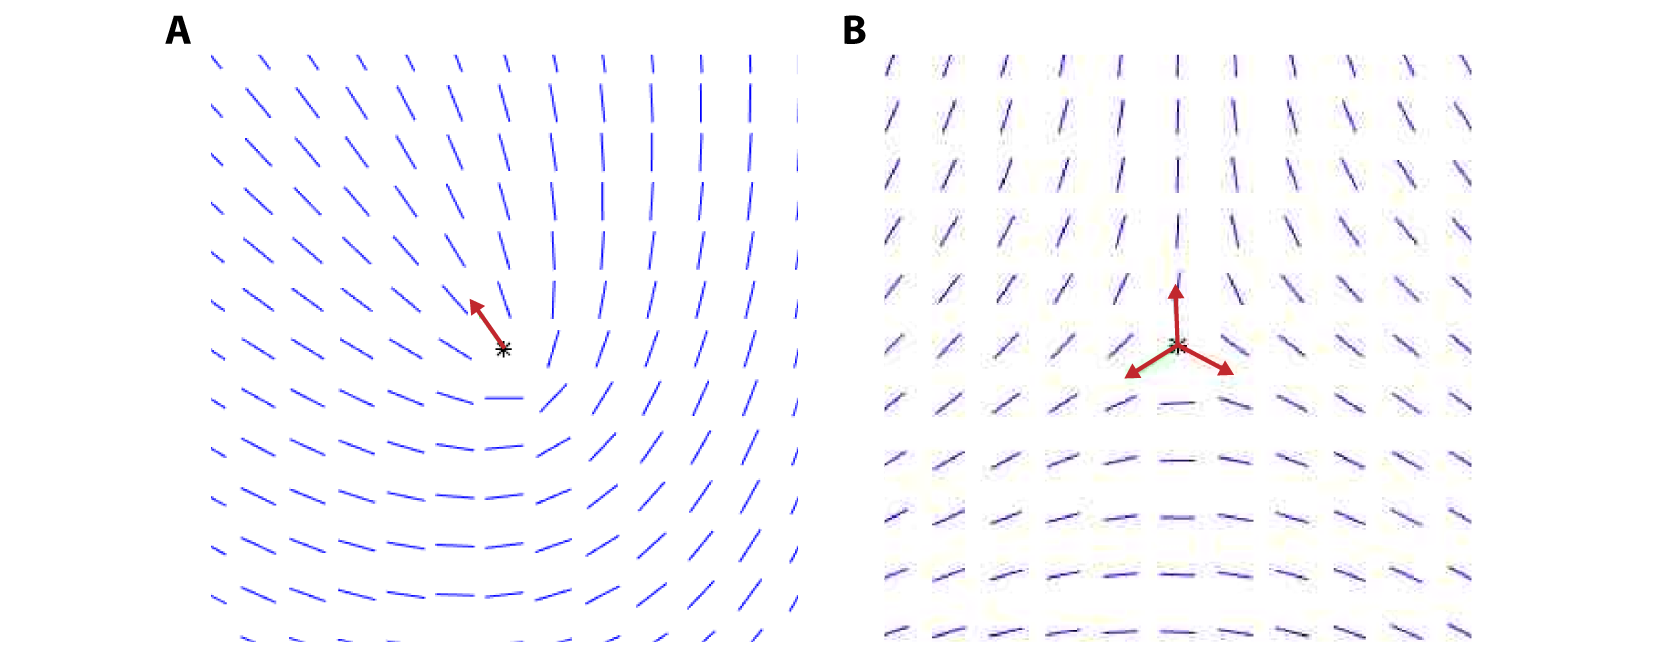
\includegraphics{figures/C7/Ch7-Figs_BasicOrients.png}
  \caption{Example director fields and axes of symmetry for an (A) $s = +1/2$ and an (B) $s=-1/2$ defect.
  The axes of symmetry were calculated with Eqs.~\ref{e:7-JSpositive}~and~\ref{e:7-JSnegative}.
  }\label{f:7-BasicOrients}
\end{figure}

Comparing the two methods to calculate the orientation of an $s = +1/2$ disclination, we have:
\begin{align}
 p_i &= \left \langle \partial_j Q_{ij}^{(\alpha)} \right \rangle_{\alpha} \nonumber \\
  &= \left \langle \partial_j \bigg(S^{(\alpha)}\bigg(n_{i}^{(\alpha)}n_{j}^{(\alpha)} - \frac{1}{2}\delta_{ij}\bigg)\bigg) \right \rangle_{\alpha} \nonumber \\
  &= \left \langle (\partial_j S^{(\alpha)}) \bigg(n_{i}^{(\alpha)}n_{j}^{(\alpha)} - \frac{1}{2}\delta_{ij}\bigg) \right \rangle_{\alpha}
      + \left \langle S^{(\alpha)} \partial_j (n_{i}^{(\alpha)}n_{j}^{(\alpha)}) \right \rangle_{\alpha} \nonumber \\
  &= \left \langle \frac{\partial_j S^{(\alpha)}}{S^{(\alpha)}} Q_{ij}^{(\alpha)}\right \rangle_{\alpha}
      + \left \langle S^{(\alpha)} \partial_j (n_{i}^{(\alpha)}n_{j}^{(\alpha)}) \right \rangle_{\alpha}\label{e:7-comparison}.
\end{align}
If we choose a contour where $S$ is constant, Eq.~\ref{e:7-comparison} becomes
\begin{equation}
  p_i = S \, b_i.
\end{equation}
Under this condition, both approaches give the same orientation.
However, in general, Eq.~\ref{e:7-LGpositive} includes additional information about the spatial variation of $S$ near the disclination.
Since the methodology in Ref~\cite{jsel} produces a tensor for both $s = \pm 1/2$ disclinations, we will use Eqs.~\ref{e:7-JSpositive}~and~\ref{e:7-JSnegative} to calculate our defect orientations.


\subsection{Experiment}
Our goal is to examine the defect orientations on the curved surface of our toroidal droplets.
However, we project our data from the surface of the toroid onto a plane, forming a 2D image from which we determine the director and the defects.
Thus, we will find the defect orientations in the 2D image and then project the defect orientations back onto our toroidal surface.
In the plane of the image, we have the Cartesian coordinate system $\{ \hat{x},\hat{y},\hat{z} \}$ with unit vectors $(1,0,0)$, $(0,1,0)$, and $(0,0,1)$, respectively.
For an arbitrary unit surface normal $\mathbf{k} = (a, b, \sqrt{1-a^2-b^2})$, we define $\hat{v} = \hat{k} \times \hat{x}/|\hat{k} \times \hat{x}|$ and $\hat{u} = \hat{v} \times \hat{k}$, giving us an orthonormal coordinate frame on the surface $\{\hat{u},\hat{v},\hat{k} \}$.

Transforming between $\mathbf{r} \in \mathbb{R}^2$ to $\mathbf{r}'$ on the surface of our toroid,
\begin{equation}
  \mathbf{r}' =
  \begin{pmatrix}
  \frac{1}{\sqrt{1-a^2}} & 0 \\
  \frac{ab}{\sqrt{(1-a^2)(1-a^2-b^2)}} & \sqrt{\frac{1-a^2}{1-a^2-b^2}}
  \end{pmatrix}
  \mathbf{r} = \bm{H}\mathbf{r}.
\end{equation}
However, since $\{ \hat{u},\hat{v}\}$ depends on $\hat{k}$, $\{ \hat{u},\hat{v}\}$ will change over the surface of our droplet, making it difficult to compare defect orientations between different points on the surface.
Instead, we will record our defect orientations on the surface of the torus in terms of a pair of curvilinear coordinate systems.
The first coordinate system is the standard toroidal coordinate system, $\{\hat{\theta}, \hat{\varphi}, \hat{r}  \}$, where $\hat{r} = \mathbf{k}$, the surface normal.
The second coordinate system is $\{\hat{\theta}', \hat{\varphi}',\mathbf{k} \}$, with $\hat{\theta}' = (\nabla K)/|\nabla K|$, and $\hat{\varphi}' = \mathbf{k} \times \hat{\theta}'$.
For a perfect toroid, the two coordinate systems are equivalent; however, in our case, the surface can be rough and our droplets are not perfectly axisymmetric.
Thus, our two coordinate systems should allow us to distinguish between global effects driven by the toroidal geometry and local effects driven by $K$.

To calculate $\hat{\theta}$ and $\hat{\varphi}$, we start by finding the central circle from our data in $\mathbb{R}^2$.
We fit circles to the outer and inner contours in the 2D image of the toroidal droplet and average these contours to get an estimate of the central circle of our toroidal droplet.
From the central circle, we can define a set of polar coordinates in the image $\{\hat{\rho}, \hat{\phi}\}$.
We project $\hat{\phi}$ onto the surface of the torus to yield $\bm{\varphi} = \bm{H}\hat{\phi}$, and then normalize to get $\hat{\varphi} = \bm{\varphi}/|\bm{\varphi}|$.
Finally, we calculate $\hat{\theta} =  \hat{\varphi} \times \mathbf{k}$ to obtain the standard toroidal coordinate system on our toroidal droplet.

To calculate $\hat{\theta}'$ and $\hat{\varphi}'$, we start by computing $\nabla K$ in the 2D image and projecting it to the surface of the toroid to get:
\begin{equation}
  \bm{\theta}' =
  \begin{pmatrix}
    \sqrt{1-a^2} & -\frac{ab}{\sqrt{1-a^2}} \\
    0 & \sqrt{\frac{1-a^2-b^2}{1-a^2}}
  \end{pmatrix}
  \nabla K = \bm{H}^{-1} \nabla K.
\end{equation}
Normalizing, we get $\hat{\theta}' = \bm{\theta}'/|\bm{\theta}'|$, and then calculate $\hat{\phi}' = \mathbf{k} \times \hat{\theta}'$.
Note that we project $\nabla K$ from the image to the surface of the toroid using $\bm{H}^{-1}$; $\nabla K$ is a covector and thus the transformation matrix is the inverse of that for a vector.

As a first attempt, we will bin the surface by $K$ and compute the order parameters in each bin.
We will use overlapping bins of constant area in the 2D image.

We start by choosing a binsize $N$, in pixels.
For a total area, $A$, in pixels, in the 2D image of the toroid, we consider a total of $A-N$ bins.
With this protocol, two adjacent bins share all but a single pixel.
We characterize each bin with $\langle K \rangle$, and then calculate the relevant order parameters in the bin using all $s = \pm 1/2$ defects in the bin over all time frames.
For the $s = +1/2$ disclinations, we calculate the polar and nematic order parameters
\begin{align}
  S_{polar} \bm{\nu} &= \frac{1}{n} \sum\limits_{\alpha=1}^n \mathbf{b}^{(\alpha)},\label{e:7-polarorder} \\
  \mathbf{Q} &= S_{nem} \left (\mathbf{n} \otimes \mathbf{n} \right ) - \frac{1}{2}\mathbb{1} = \frac{1}{n} \sum\limits_{\alpha=1}^n \mathbf{b}^{(\alpha)} \otimes \mathbf{b}^{(\alpha)} - \frac{1}{2}\mathbb{1}\label{e:7-nematicorder},
\end{align}
where $S_{polar}$ and $S_{nem}$ is the magnitude of the order and $\bm{\nu}$ and $\mathbf{n}$ unit vectors describing the direction of the order, for polar order and nematic order, respectively.
We note that Eq.~\ref{e:7-nematicorder} is equivalent to Eq.~\ref{e:2-2DOrderRaw} and Eq.~\ref{e:2-2DOrderDiag}.

For the $s = -1/2$ disclinations, we take the orientation of $T_{ijk}$ to be the angle $\phi_0 \in [-\pi/3,\pi/3)$, the orientation of one of the three axes of symmetry of an $s = -1/2$ disclination.
Consider $\mathbf{n} = (n_x \hat{x}, n_y \hat{y})$ surrounding an $s = -1/2$ disclination, where $\theta = \arctan (y/x)$ is the polar angle describing the position.
Then, if $\phi = \theta + \phi_0$ describes the director orientation, we can write the director field surrounding the disclination as $\mathbf{n} = (\cos(\phi/2)\hat{x},-\sin(\phi/2)\hat{y})$.
Computing $T_{ijk}$ according to Eq.~\ref{e:7-JSnegative} and averaging over all $\theta$, we have:
 \begin{align}
   \langle T_{ij1}(\theta) \rangle_{\theta} &=
        \frac{3}{4}\begin{pmatrix}
          \cos \phi_0 & -\sin \phi_0 \\
          -\sin \phi_0 & -\cos \phi_0
        \end{pmatrix}\nonumber \\
  \langle T_{ij2}(\theta) \rangle_{\theta} &=
       \frac{3}{4}\begin{pmatrix}
         -\sin \phi_0 & -\cos \phi_0 \\
         -\cos \phi_0 & \sin \phi_0
       \end{pmatrix}\label{e:7-TijkBIG}
 \end{align}
From Eq.~\ref{e:7-TijkBIG}, we can now obtain $\phi_0$ from $\langle T_{ijk}(\theta) \rangle_{\theta}$ via:
\begin{equation}\label{e:7-phi0Calc}
  \phi_0 = \arctan \left ( \frac{\langle T_{222}(\theta) - T_{121}(\theta) - T_{112}(\theta) - T_{211}(\theta)  \rangle_{\theta}} {\langle T_{111}(\theta) - T_{221}(\theta) - T_{122}(\theta) - T_{212}(\theta)  \rangle_{\theta}} \right).
\end{equation}

Now, we use $\phi_0$ to calculate the bond-angle order parameter for three-fold symmetry for the $s = -1/2$ disclinations in the bin
\begin{equation}\label{e:7-hexorder}
  S_{bond} \exp(i 3 \Phi_o) = \frac{1}{n}\sum\limits_{\alpha = 1}^n \exp (i 3 \phi_o^{(\alpha)}),
\end{equation}
where $S_{bond}$ is the magnitude of the order and $\Phi_o$ is an angle giving the orientation of the order.
\begin{figure}
  \centering
  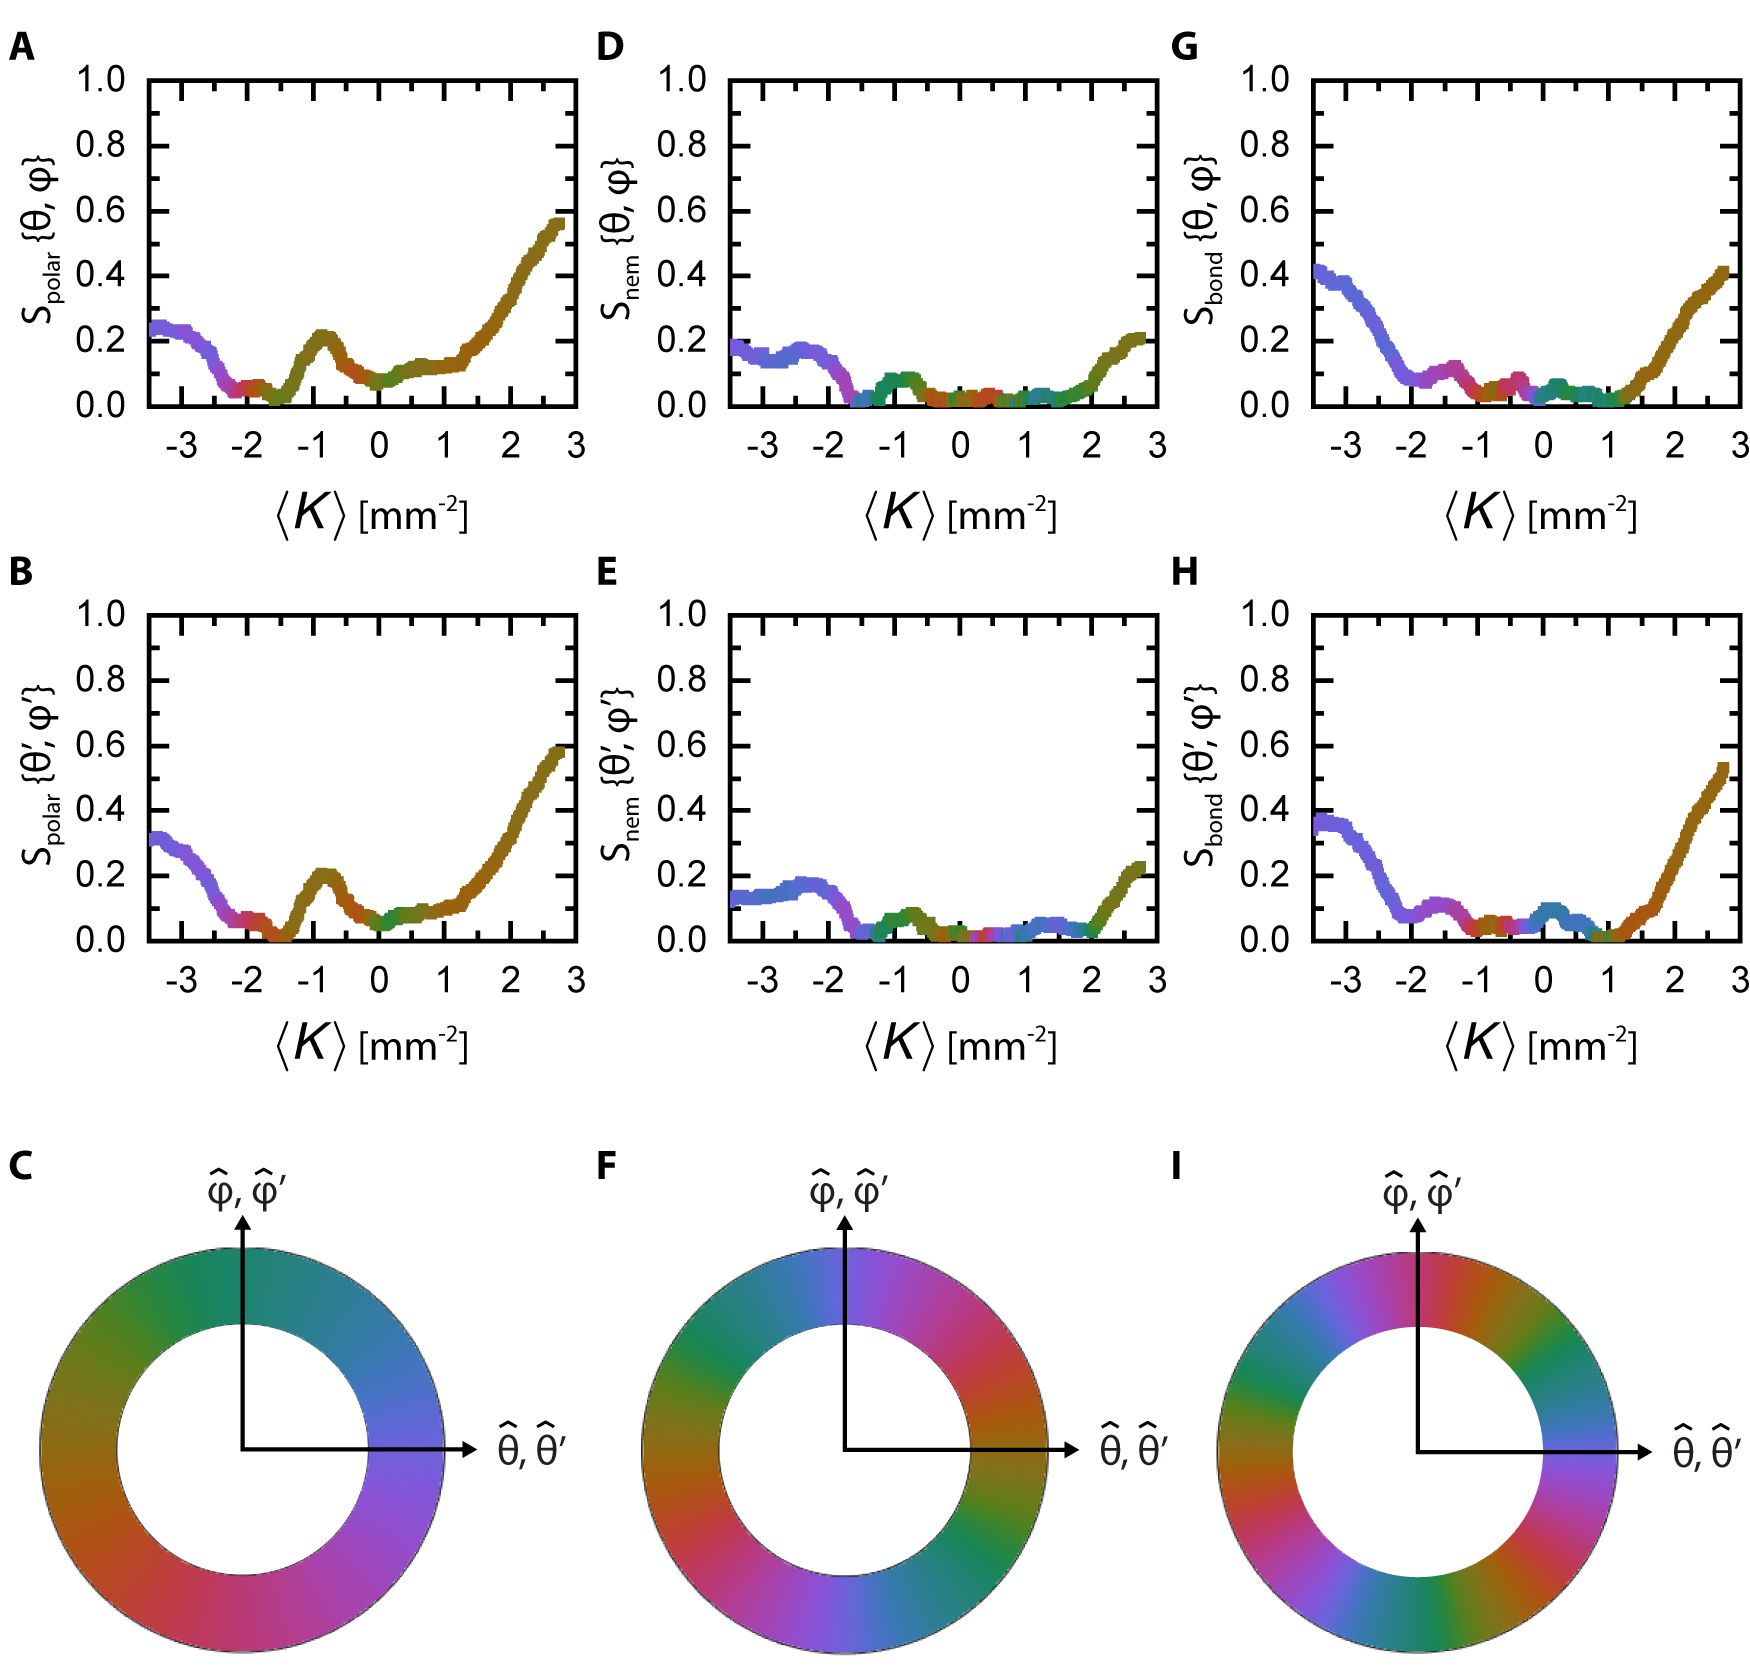
\includegraphics{figures/C7/Ch7-Figs_Orient_MeanK.png}
  \caption{$s = \pm 1/2$ defect ordering on a toroid with $\xi = 2.4$, $a = 268$ $\upmu$m, and an ATP concentration of 144 $\upmu$M.
  Magnitude and direction of (A--C) polar and (D--F) nematic order calculated for the $s = +1/2$ defects and (G--I) three-fold bond angle order calculated for the $s = -1/2$ defects.
  The order in (A,D,G) and (B,E,H) is calculated for the $\{\theta,\varphi \}$ and the $\{\nabla K = \theta',\varphi' \}$ coordinate systems, respectively, with (C,F,I) indicating the color scales used to denote orientation.
  }\label{f:7-Orient_MeanK}
\end{figure}

For an example toroid with with $\xi = 2.4$, $a = 268$ $\upmu$m, and an ATP concentration of 144 $\upmu$M, we plot the magnitude and orientation of the nematic and polar order for the $s = +1/2$ defects and the three-fold bond order for the $s = -1/2$ defects as a function of the mean Gaussian curvature in each bin  in Figure~\ref{f:7-Orient_MeanK}(A--C), Figure~\ref{f:7-Orient_MeanK}(D--F), and Figure~\ref{f:7-Orient_MeanK}(H--J) respectively.
We see that for both the $\{\Theta,\varphi\}$ [Figure~\ref{f:7-Orient_MeanK}(A,D,G)] and the $\{ \nabla K = \theta',\varphi' \}$ [Figure~\ref{f:7-Orient_MeanK}(B,E,H)] coordinate systems, the $s = \pm 1/2$ defects exhibit order in the regions where the magnitude of $K$ is larger.
Interestingly, we note that the $s = +1/2$ defects exhibit polar order on our toroidal droplets, rather than nematic order seen in flat space~\cite{RN27}.
Since we consider the defects at all time points when calculating the order, Figure~\ref{f:7-Orient_MeanK} reflects a persistent steady state.
In addition, the we see that the direction of the order is different in regions of negative and regions of positive Gaussian curvature.
In regions where $K > 0$, the $s = +1/2$ defects align along $-\hat{\theta}$, consistent with the idea that the $s = +1/2$ defects migrate towards $\theta = \pi$ in order to minimize their contribution to the free energy.
However, in regions where $K < 0$, the $s = +1/2$ defects align along $\hat{\theta}$, the opposite of what we expect; this indicates that on average, $s = +1/2$ defects in regions near the hold of the torus move further towards $\theta = 0$.
We note that even if the $s = +1/2$ defects want to move towards the hole, this is still consistent with curvature-induced defect unbinding provided that the $s = -1/2$ defects migrate towards the hole at a higher rate than the $s = +1/2$ defects.
Repeating this analysis for the remainder of our toroids, our preliminary results indicate that the $s = +1/2$defects posses steady state polar order, the $s = -1/2$ defects posses steady state three-fold bond angle order, and that the magnitude of the order grows with increasing $|K|$ for both defect species.

To investigate the origin of this order, we plot the polar order for the $s = +1/2$ defects and the three-fold bond angle order for the $s = -1/2$ defects against the mean defect density and against the mean $|K|$ in each bin in Figure~\ref{f:7-Orient_PolarHex}(A--D) and Figure~\ref{f:7-Orient_PolarHex}(F--I), respectively.
We see from the plotting the order against the mean defect density in each bin, that the magnitude of the order grows as the defect density decreases [polar order, Figure~\ref{f:7-Orient_PolarHex}(A.C) and three-fold bond angle order, Figure~\ref{f:7-Orient_PolarHex}(F,H)]; this is the opposite of the results in flat space~\cite{RN27}.
We also see that the magnitude of the defect order grows with increasing $|K|$ [polar order, Figure~\ref{f:7-Orient_PolarHex}(B,D) and three-fold bond angle order, Figure~\ref{f:7-Orient_PolarHex}(G,I)]; this makes intuitive sense as the gradient of the Gaussian curvature reflects the change in the ``background charge'' influencing the defects.
\begin{figure}
  \centering
  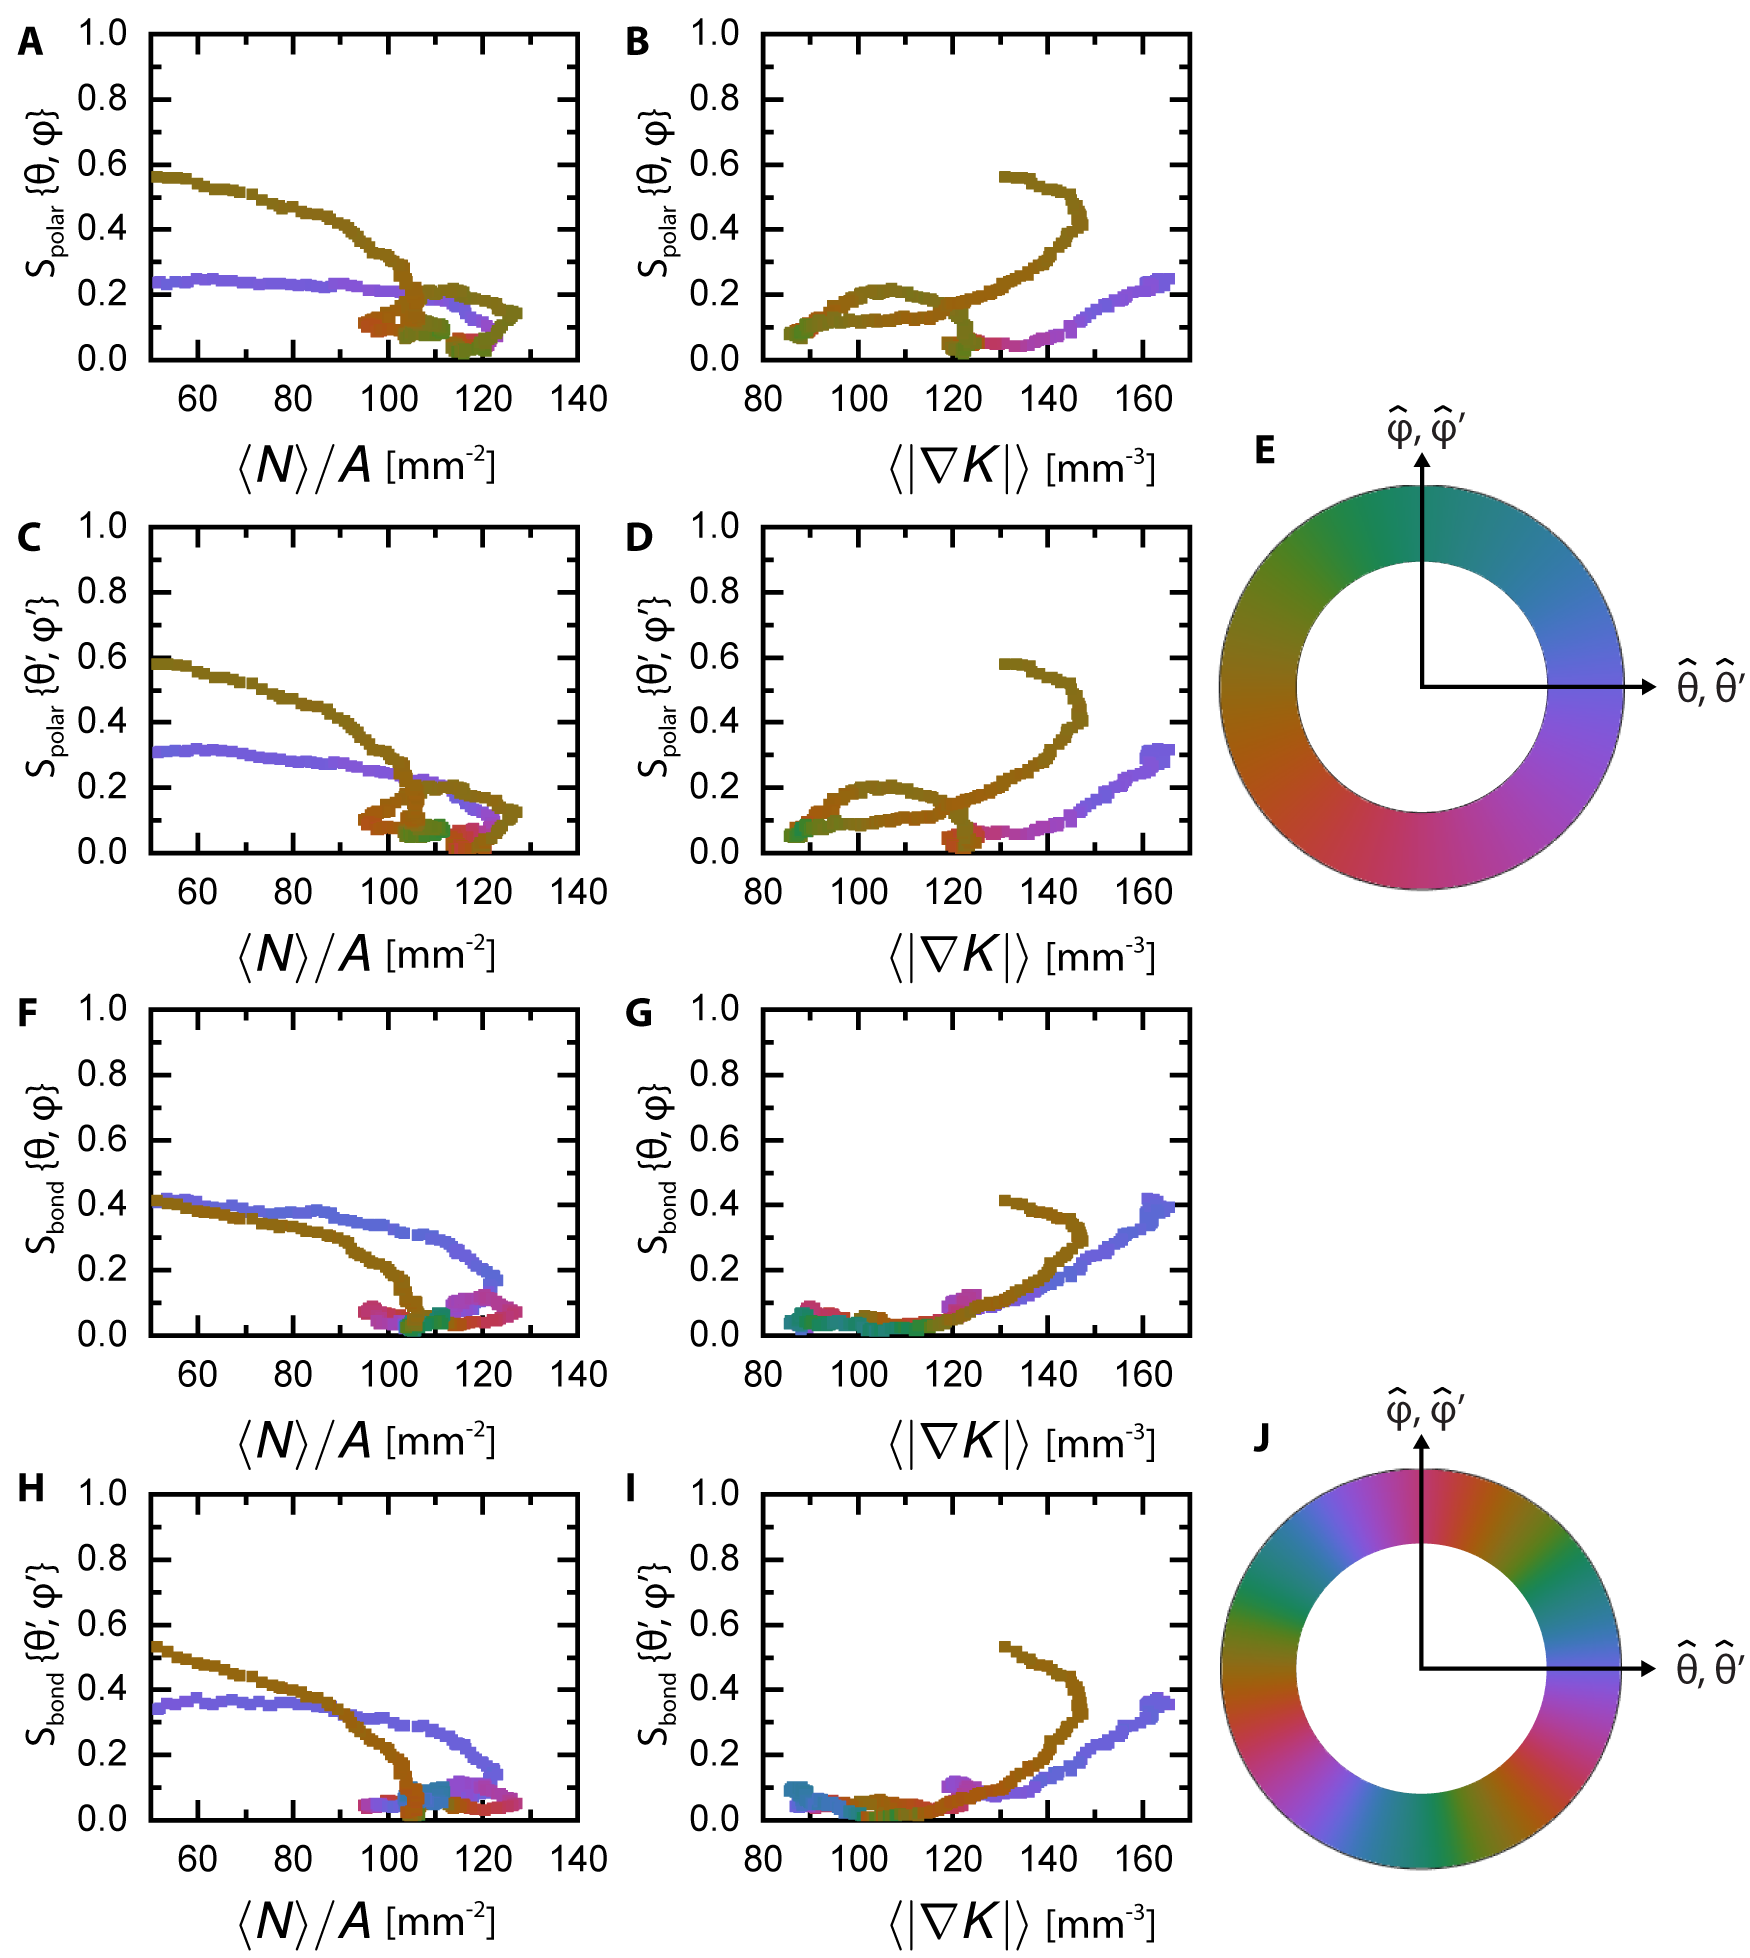
\includegraphics{figures/C7/Ch7-Figs_Orient_PolarHex.png}
  \caption{$s = \pm 1/2$ defect order plotted as a function of the mean defect density and of the magnitude of the gradient of the Gaussian curvature.
  Magnitude and direction of the (A--D) polar order for the $s = +1/2$ defects and the (F--I) three-fold bond angle order for the $s = -1/2$ defects.
  (A,B) and (F,G) are calculated in the $\{\theta,\varphi \}$ coordinate system, while (C,D) and (H,I) are calculated in the $\{ \nabla K = \theta',\varphi' \}$ coordinate system.
  The magnitude and direction of the order are plotted in (A,C,F,H) and (B,D,G,I) as a function of the mean defect density and of the mean magnitude of the gradient of the Gaussian curvature, respectively.
  The polar and three-fold bond angle color scales are displayed in (E,J), respectively.
  }\label{f:7-Orient_PolarHex}
\end{figure}


\subsection{Future Work}
To understand the nature of the ordering on the toroidal droplets, we need more data that focuses on the regions of the toroids that have a large Gaussian curvature magnitude.
These regions are where we see the ordering arise and where we have the least amount of data.
We are currently taking more data that looks specifically at these highly curved regions.
In addition, we are currently taking data on cylindrical surfaces in order to better understand how the global properties of a surface affect the defect ordering.
In addition, now that we see that there is a persistent steady-state in the defect orientations, we are analyzing smaller time windows to obtain the fluctuations in the orientation.

We also wish to understand defect orientation correlations in space at a given time.
To do this, we need to be able to calculate discrete geodesics on the surface of the torus.
We are currently working on implementing the algorithms in Refs.~\cite{RN322,RN323}.



\section{Determining the saddle-splay elastic constant: current status}
It is difficult to measure saddle-splay because it is difficult to achieve a pure saddle-splay distortion in a nematic volume [see Eq.~\ref{e:2-FrankPhysicalExpansion}].
In addition, since the saddle-splay distortion in the bulk is intimately connected with the director behavior on the boundary of the material, there is concern that anchoring and surface elastic terms could prevent an accurate measurement of $K_{24}$~\cite{RN191,RN55,sidky2018silico}.
Finally, there are discrepancies concerning the coefficient associated with the saddle-splay distortion, with
$-(1/2)(K_{22} + K_{24})\nabla \cdot (\mathbf{n}\nabla \cdot \mathbf{n} + \mathbf{n} \times \nabla \times \mathbf{n})$,
$-(1/2)K_{24}\nabla \cdot (\mathbf{n}\nabla \cdot \mathbf{n} + \mathbf{n} \times \nabla \times \mathbf{n})$,
and $-K_{24}\nabla \cdot (\mathbf{n}\nabla \cdot \mathbf{n} + \mathbf{n} \times \nabla \times \mathbf{n})$ all found in the literature.
As a result, the published measurements of $K_{24}$ often differ substantially.
For example, the reported measurements of $K_{24}$ for 5CB, the most common thermotropic NLC in the literature, vary from $\approx K$ in a 1-constant approximation  to $3.1 K_{22}$ [see Table~\ref{t:7-K24}]~\cite{RN24,allender1991determination,polak1994optical,sparavigna1994periodic}.
Even after correcting for notational differences and representing the saddle splay distortion as in Eq.~\ref{e:2-FrankFinalExpansion}, we see in Table~\ref{t:7-K24} that the published measurements are in general imprecise due to either a large error or a reliance on a 1-constant approximation.
Furthermore, the concerns in the literature that any measurement of $K_{24}$ is always affected by interactions between the nematic and the confining volume cast further doubt on the measurements in Table~\ref{t:7-K24}~\cite{RN55,RN191,sidky2018silico}.
\begin{table}[t]
  \centering
  \caption{Experimentally-obtained values for $K_{24}$ using 5CB for four literature sources, both as reported and after recasting the saddle-splay distortion in the form: $-(1/2)(K_{22} + K_{24})\nabla \cdot (\mathbf{n}\nabla \cdot \mathbf{n} + \mathbf{n} \times \nabla \times \mathbf{n})$.}
  \begin{tabular}{l c l}
    & {\bf As reported} & \\
    \hline
    Authors & $K_{24}/K_{22}$ & Notes \\
    \hline
    Allender \emph{et. al.}~\cite{allender1991determination} & $1.1 \pm 0.9$ & Used 1-constant approximation\\
    Polak \emph{et. al.}~\cite{polak1994optical} & $3.1 \pm 4.4$ \\
    Sparavigna \emph{et. al.}~\cite{sparavigna1994periodic} & $0.994 \pm 0.006$ & Used 1-constant approximation \\
    Pairam \emph{et. al.}~\cite{RN24} & $1.02 \pm .02$ \\
    & {\bf Corrected notation} & \\
    \hline
    Authors & $K_{24}/K_{22}$ & Notes \\
    \hline
    Allender \emph{et. al.}~\cite{allender1991determination} & $1.2 \pm 0.8$ & Used 1-constant approximation. \\
    Polak \emph{et. al.}~\cite{polak1994optical} & $2.5 \pm 3.0$ \\
    Sparavigna \emph{et. al.}~\cite{sparavigna1994periodic} & $0.994 \pm 0.006$ & Used 1-constant approximation.\\
    Pairam \emph{et. al.}~\cite{RN24} & $1.04 \pm 0.04$ \\
  \end{tabular}
  \label{t:7-K24}
\end{table}


\subsection{Prior estimates in tori}
Recent work in NLC toroids with degenerate planar anchoring revealed the coupling between the saddle-splay distortion and the curvature of the bounding surface [see Eq.~\ref{e:2-K24SurfCouple}]~\cite{RN24,RN59}.
This coupling was used to make precise estimates of $K_{24}$ not only in 5CB but also in the LCLCs SSY~\cite{RN191,RN293} and DSCG~\cite{RN293} confined in cylindrical capillaries.
To illustrate this estimate, we refer to the example illustrated in Section 4.1 of a linear twist ansatz in a torus where $\xi \rightarrow \infty$.
Taking the values of the twist parameter, $\omega$, that minimize the free energy [Eq.~\ref{e:4-omegaMinFFE}] and substituting into the expression for the twist angl, $\tau$ [Eq.~\ref{e:4-twistAngle}], we have:
\begin{equation}
  K_{24} = K_{22} + \frac{K_{33}}{2}\sin ^2 \left( \frac{\tau}{2} \right ).\label{e:7-twistFuntionK24}
\end{equation}
Since the values of $K_{22}$ and $K_{33}$ are easy to establish independently, Eq.~\ref{e:7-twistFuntionK24} provides a relation between a single measurement of a twist angle to the value of $K_{24}$ for a given NLC.
For example, using the value of $K_{24}$ measured in Ref.~\cite{RN24}, $K_{24} = (1.04 \pm 0.04) K_{22}$, we calculate that $\tau_{\xi \rightarrow \infty} = 19^{\circ} \, [+ 8^{\circ}, - 19^{\circ}]$.

\subsection{Results from spherical drops}
Prior work with spherical emulsion droplets of 5CB in phosphate-buffered saline (PBS) with various ionic strengths found a size dependent configuration, with bipolar configurations observed for droplets with radius $R \gtrsim 1$ $\upmu$m and radial configurations for $R \lesssim 1$ $\upmu$m~\cite{miller2013influence}.
As a potential explanation, the authors considered the Frank-Oseen free energy for a radial droplet and a bipolar droplet in the presence of degenerate planar anchoring:
\begin{align}
  F_{radial} &= 8 \pi K_{11} R - 4 \pi (K_{22} + K_{24}) R + 2 \pi W R^2\label{e:7-FFEradial} \\
  F_{bipolar} &= 5 \pi K_{11} R - 2 \pi (K_{22}+ K_{24}) R,\label{e:7-FFEbipolar}
\end{align}
where $F_{anchoring} = (1/2) W (\mathbf{n} \times \mathbf{k})^2$ is the single-constant Rapini-Papoular energy for degenerate planar anchoring, with $W$ the strength of the anchoring and $\mathbf{k}$ the surface normal.
Comparing these free energies, they subtract Eq.~\ref{e:7-FFEbipolar} from Eq.~\ref{e:7-FFEradial} with $2 K_{22} = K_{11}$ for 5CB:
\begin{equation}
  \Delta F_{trans} = 2\pi R (2 K_{22}-K_{24} + W R).\label{e:7-FFEtrans}
\end{equation}
If $K_{24} > 2 K_{22}$, we see that bringing $R$ small enough will eventually cause $\Delta F_{trans}$ to become negative, indicating that a radial structure has a lower free energy than a bipolar structure.
From E.~\ref{e:7-FFEtrans}, Ref.~\cite{miller2013influence} proposed saddle-splay as responsible for the size-dependent structures observed.
While Table~\ref{t:7-K24} has measurements of $K_{24} > 2 K_{22}$, such a value of $K_{24}$ also implies that cylindrical or toroidal confinement of 5CB would result in a highly twisted configuration, far more so than the values measured in Ref.~\cite{RN24}.

Recently, we found that a similar bipolar-to-radial transition can be induced in 5CB emulsion droplets in water with 1\% w/w PVA by bringing the temperature close to $T_{NI}$, the isotropic-nematic phase transition temperature.
This transition is shown in Figure~\ref{f:7-Emulsion_Eth}(A--C) for a sample with multiple droplets, and in Figure~\ref{f:7-Emulsion_Trans}(A--E) for a single droplet~\cite{nayani2017role}.
We observe the transition at $\tilde{T} \gtrsim 0.995 T_{NI}$, where $\tilde{T} = T/T_{NI}$ is the reduced temperature~\cite{nayani2017role}.
We use Jones Calculus to simulate bipolar droplets with varying $\Delta N$, and compare the number of fringes in the simulated images with the number of fringes in our experimental images.
This process is shown in Figures~\ref{f:7-Emulsion_Trans}(A--C) for the experimental OPM images and Figure~\ref{f:7-Emulsion_Trans}(F--H) for the simulated images as a function of increasing $\tilde{T}$.
By matching the number of fringes, we can determine the birefringence, and therefor the sclar order paramter, $S$, in our experiments as a function of $\tilde{T}$~\cite{nayani2017role}.
We find that the relationship derived from the bipolar droplets agrees well with Raman scattering data on pure 5CB, as plotted in Figure~\ref{f:7-Emulsion_Trans}(I), indicating that the bipolar-to-radial transformation occurs not only at a repeatable $\tilde{T}$, but also at a repeatable $S$~\cite{nayani2017role}.
However, from this data we cannot distinguish betwen an efect driven by the absolute temperature or an effect driven by the reduced temperature.
\begin{figure}
  \centering
  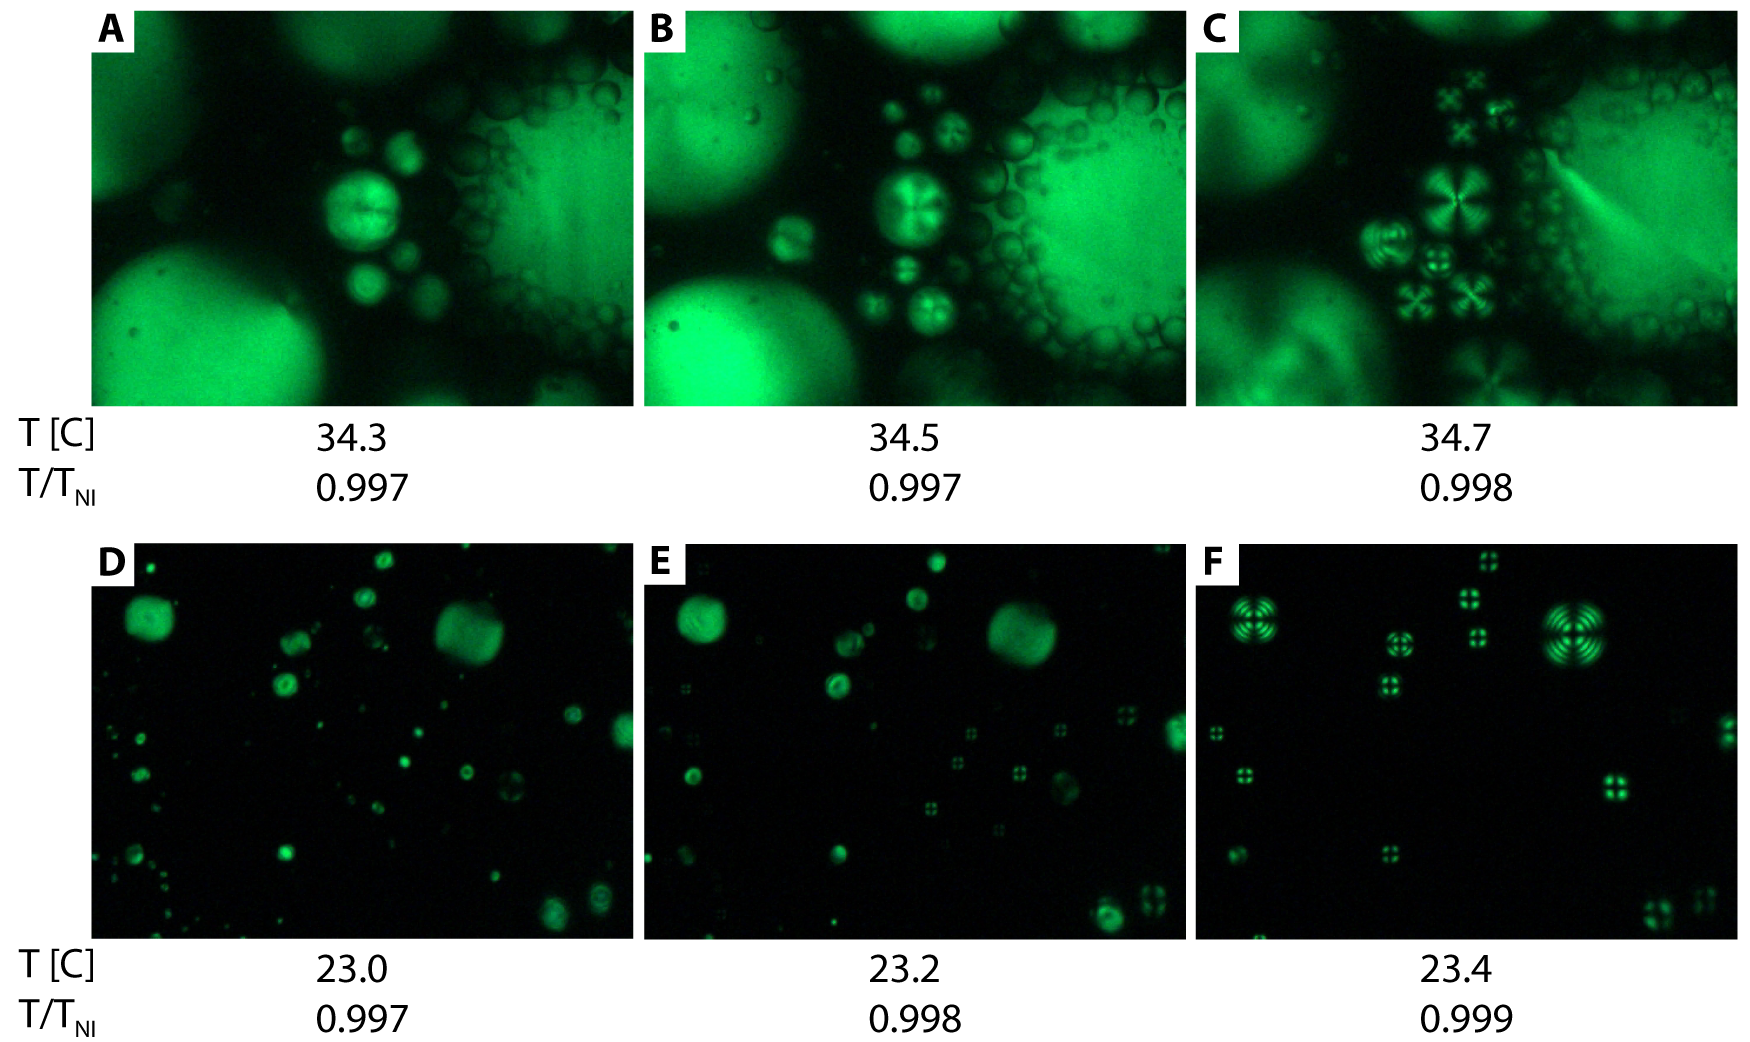
\includegraphics{figures/C7/Ch7-Figs_Emulsion_Eth.png}
  \caption{OPM textures of an emulsion of 5CB undergoing a bipolar-to-radial transformation.
      (A--C), The outer medium consists of 99\% w/w Millipore water with 1\% w/w PVA.
      (D--F), The outer medium consists of 69\% w/w Millipore water, 30\% w/w Ethanol, and 1\% w/w PVA.
      In all images the absolute and reduced temperature are displayed below the image.
      The scale bar is: 50 $\upmu$m.
      }\label{f:7-Emulsion_Eth}
\end{figure}

We test this by making 5CB emulsion droplets in mixtures of water and ethanol, where the concentration of PVA is always 1\% w/w.
The addition of ethanol to the continuous phase lowers $T_{NI}$; at concentrations of ethanol greater than 30 \% w/w, we find that 5CB is isotropic at room temperature.
Irrespective of the concentration of ethanol, we find that the transition occurs consistantly at $\tilde{T} \gtrsim 0.995 T_{NI}$, shown in Figure~\ref{f:7-Emulsion_Eth}(D--F) for an outer medium of 1\% w/w PVA, 30\% w/w ethanol, and 69\% w/w Millipore water.
In addition, while we observe that small droplets tend to transform before large droplets, we do not have the sensitivity to quantitatively measure the transition as a function of size.
This confirms that the transition is not a function of the absolute temperature, but depends on the reduced temperature through the scalar order parameter.
Furthermore, the continuous phase here is very similar to that used in Ref.~\cite{RN24} to measure $K_{24} =(1.04 \pm 0.04)K_{22}$ for 5CB, indicating that it is not likely that saddle-splay is solely responsible for the bipolar-to-radial transition.
However, we note that if saddle-splay truly cannot be measured without influence from the confining phase, then we would need to repeat these measurements in the identical outer phase to Ref~\cite{RN24}.
When we do this, we find that irrespective of the carbopol or ethanol concentration in the outer phase, all our spherical emulsions demonstrate a bipolar-to-radial transition at $\tilde{T}\gtrsim 0.995 T_{NI}$.
Finally, we note that while we generally assume that the ratios of the elastic constants do not change with temperature, Eqs.~\ref{e:2-LdGFrankRelationsA}--\ref{e:2-LdGFrankRelationsD}, indicate that there will be some variation, possibly reaching a regime where $K_{24}$ could drive the bipolar-to-radial transition.
\begin{figure}
  \centering
  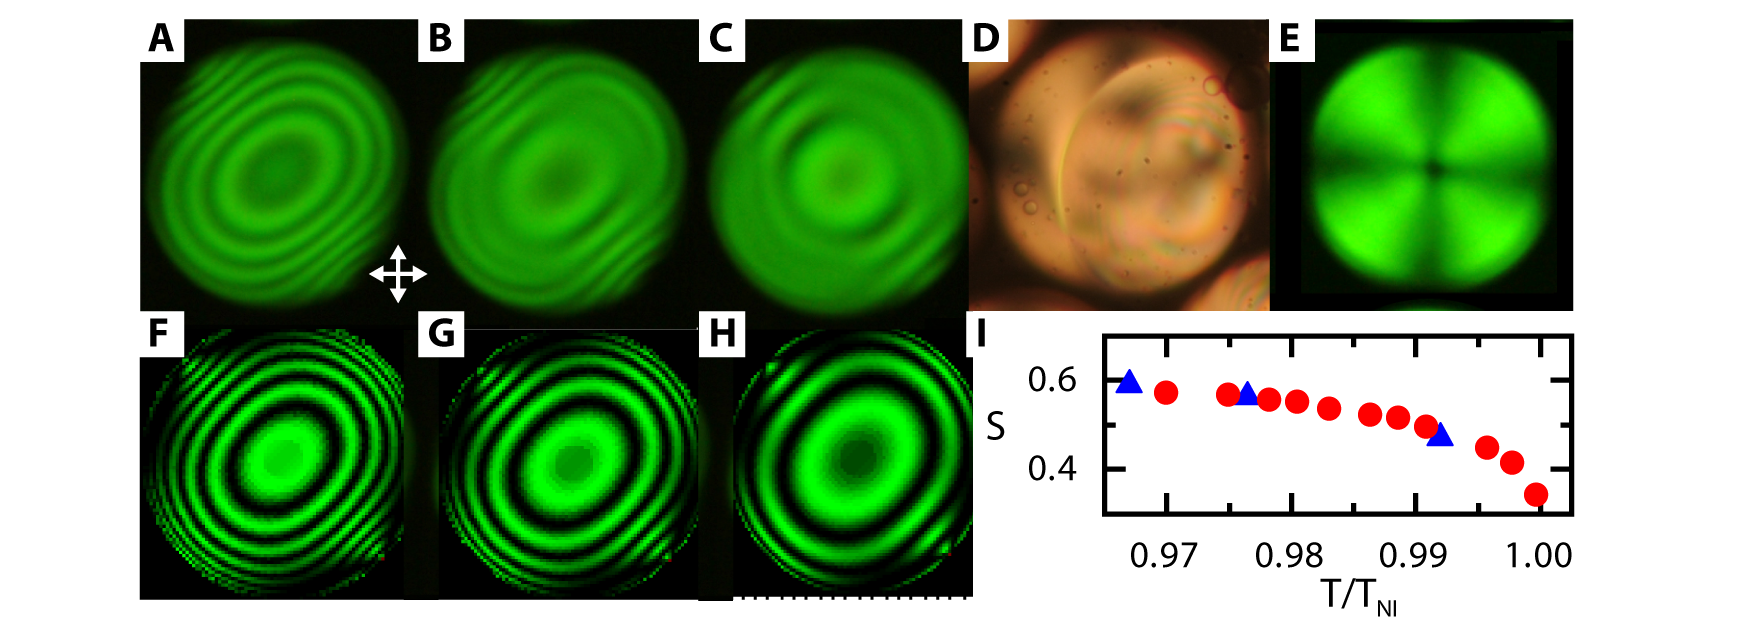
\includegraphics{figures/C7/Ch7-Figs_Emulsion_Trans.png}
  \caption{The transition from bipolar-to-radial happens as the order paramter decreases.
    (A--E), Experimental images showing how a 40 $\upmu$m diameter bipolar droplet transforms into a raial droplet.
    As the reduced temperature increases, the number of fringes in the (A--C) bipolar OPM textures decrease.
    The saturn ring mediated the bipolar-to-radial transformation is clearly visible under bright-field illumination in (D), with the final radial structure visible in the OPM texture in (E).
    (F--H), Simulated OPM textures of bipolar droplets with varing $\Delta n$; the $\Delta n$ were chosen to match the number of fringes in the experimental OPM textures in (A--C), respectively.
    (I), Plot of the scalar order parameter vs. the reduced temperature with data from Raman scattering measurements (${\color{red} \bullet}$) and from matching the simulated and experimental OPM textures (${\color{blue} \blacktriangle}$)
     }\label{f:7-Emulsion_Trans}
\end{figure}

\subsection{Distinguishing $K_{24}$ and surface contributions using twist angle and temperature}
To test whether the temperature scaling of $K_{24}$ could result in $K_{24} > 2 K_{22}$, we will measure the the twist angle of 5CB confined under degenerate planar anchoring to cylindrical structures.
We make cylindrical structures by inserting a 27 Ga (410  $\upmu$m OD) needle completely into a yield stress fluid and then slowly removing the needle as we pump 5CB into the void left by the withdrawing needle.
The needle is 2 inches long, and we control the speed of withdrawl using a mechanical stage controlled by a MATLAB script.
We set the volume flowrate of the 5CB between 0\% and 10\% in excess of the volume/time vacated by the needle; flowrates in this range generally produce smooth, cylindrical structures, as shown in the example image in Figure~\ref{f:7-CapStructure}(A).
Currently, we have tested cylindrical structues in yield-stress media containing 1\% w/w PVA, 3\% w/w Glycerol, 0\%--2\% w/w carbopol, 0\%--30\% w/w ethanol, with the remaining percentage taken by Millipore water.
Example OPM textures of the structure in Figure~\ref{f:7-CapStructure}(A) are shown in Figures~\ref{f:7-CapStructure}(B,C), while images for a structure made in a yield-stress medium with no ethanol are shown in Figures~\ref{f:7-CapStructure}(D,E).
We measure the twist angle by first varying both P and A until the minimum transmitted intensity is reached.
We then fix P, measure the transmitted intensity every 5$^\circ$ in the A orientation, and fit the resulting data to the expected transmitted intensity for a twisted nematic cell [Eq.~\ref{e:4-tn}].
For the two examples in Figures~\ref{f:7-CapStructure}(B,C) and Figures~\ref{f:7-CapStructure}(D,E), we measure a twist angles of $\tau = 13^{\circ} \pm 1^{\circ}$ and $\tau = 7^{\circ} \pm 1^{\circ}$, respectively.
Our preliminary data show twist angles consistent with the value of $K_{24}$ measured in Ref.~\cite{RN24}, regardless of the concentration of carbopol or ethanol in the outer yield-stress medium.
We are currently working on measurements of twist angle as a function of temperature.
However, we note that our samples with higher concentrations of ethanol have a lower clearing point and thus the measurements corresponds to a higher $\tilde{T}$, indicating that it is not likely that increasing temperature for a given sample will cahuse $K_{24} \approx 2 K_{22}$.
\begin{figure}
  \centering
  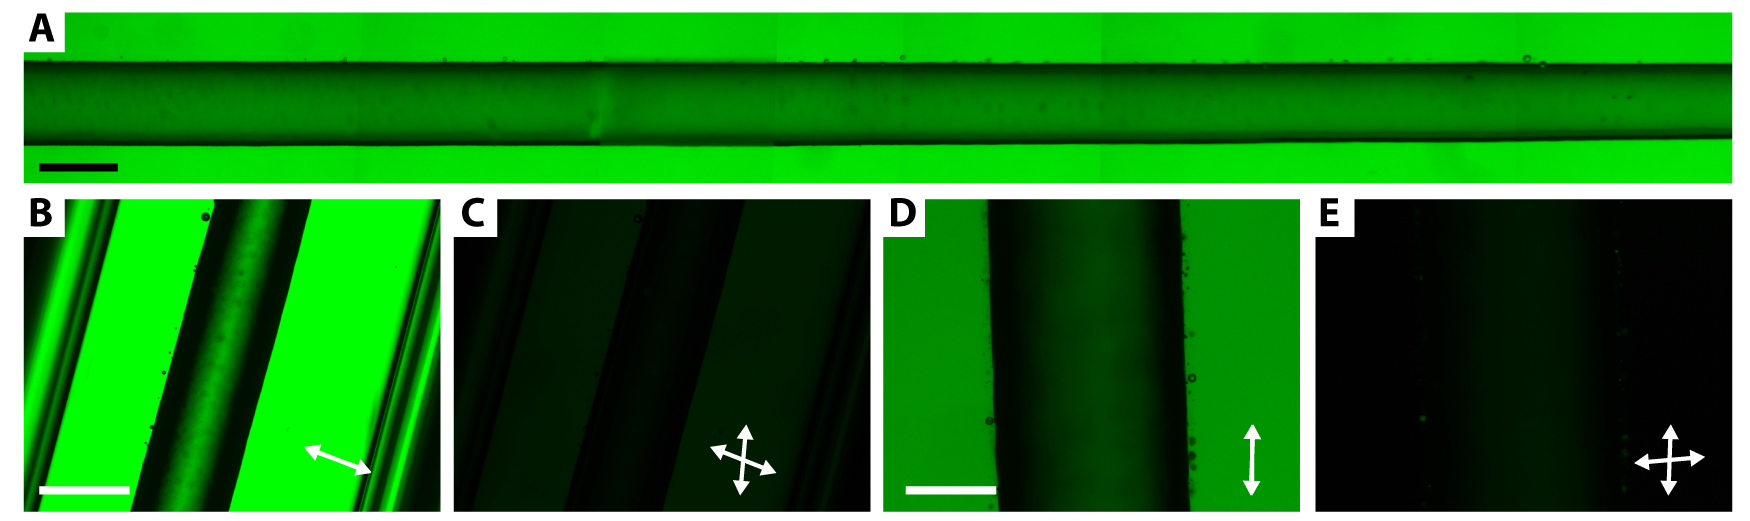
\includegraphics{figures/C7/Ch7-Figs_CapStructures.png}
  \caption{Cylindrical structures of 5CB in a yield-stress material.
  (A), Bright-field image of a cylindrical structure of 5CB in a yield-stress medium consisting of 1\% w/w PVA, 1.5\% w/w Carbopol, 3\% w/w glycerol, 30\% w/w ethanol, 64.5 w/w \% Millipore water.
  (B--E), OPM textures of cylindrical structures of 5CB with (B,D) having aligned P and A, and (C,E) having P and A oriented for minimum transmission through the 5CB structure.
  (B,C) are a section of the structure in (A), while (D,E) are a section from a structure in an outer medium consisting of 1\% w/w PVA, 1.8\% w/w Carbopol, 3\% w/w glycerol, 94.2 w/w \% Millipore water.
  Scale bar for (A--C) is 500 $\upmu$m; for (D,E) the scale bar is 250 $\upmu$m.
  }\label{f:7-CapStructure}
\end{figure}


%%%%%%%%%%%%%%%%
% Appendices
%%%%%%%%%%%%%%%%

%!TEX root = thesis.tex
\begin{appendices}

%Some Table of Contents entry formatting
\addtocontents{toc} {\protect\renewcommand{\protect\cftchappresnum} {\appendixname\space}}
\addtocontents{toc}{\protect\renewcommand{\protect\cftchapnumwidth}{6em}}

%Begin individual appendices, separated as chapters

\chapter{A brief introduction to Differential Geometry}\label{a:A}
This appendix briefly introduces some useful ideas and definitions in differential geometry.
I follow Refs.~\cite{RN35,RN266} and limit the discussion to the concepts needed to follow the main text of this thesis.
While much of what follows can be generalized to $n$-dimensions, I will primarily discuss concepts in 3 or fewer dimensions.



\section{Manifolds and (hyper)surfaces}
A \emph{manifold} is a space that locally looks like Euclidean space.
Trivially, this implies that Euclidean space is a manifold.
If the manifold is differentiable, then we can also do calculus on the manifold.
Euclidean space is differentiable; in fact, most of us learned to do calculus in 3D Euclidean space, $\mathbb{R}^3$, with the global coordinate system, $(x^1,x^2,x^3)$.
This easily generalizes to $n$-dimensional Euclidean space, $\mathbb{R}^n$, with its global coordinate system, $(x^1,x^2, \ldots , x^n)$.
Now, we define a 2D surface embedded in $\mathbb{R}^3$ as some subset of $\mathbb{R}^3$ that locally looks like $\mathbb{R}^2$.

Since our 2D surface locally resembles 2D Euclidean space, we see that the surface itself qualifies as a manifold.
In fact, generalizing this definition gives us \emph{submanifolds}, a subset of a manifold which itself is a manifold.
More formally, let the subset $\mathbb{X} = \mathbb{X}^n \subset \mathbb{R}^{n + p}$ be the $n$-dimensional submanifold of $\mathbb{R}^{n+p}$ if $\mathbb{X}$ can locally be described by writing $p$ of the coordinates differentially in terms of the $n$ remaining coordinates.
Explicitly, for $r \in \mathbb{X}$, a neighborhood of $r$ on $\mathbb{X}$ can be described by the local coordinates $(\mathbf{u},\mathbf{v}) = (u^1,\ldots,u^n,v^1,\ldots,v^p)$ in $\mathbb{R}^{n+p}$ where $v^j = f^j(u^1,\ldots,u^n)$, with $j = 1,\ldots,p$, and $f$ a smooth function.

Thus, we define a surface as a 2D submanifold of $\mathbb{R}^3$ such that $v = f(u^1,u^2)$, where $u^1$ and $u^2$ are coordinates that parameterize the surface and $v$ is the third coordinate in $\mathbb{R}^3$.
Similarly, a curve is a 1D submanifold of $\mathbb{R}^3$ where $v = g^1(u^1) = g^2(u^2)$ and a planar curve is a 1D submanifold of $\mathbb{R}^2$ where $v = f(u)$.
Note that this definition implies that a curve in general can be considered part of a surface, with a planar curve restricted a globally flat surface.
If we define the codimension of a submanifold $\mathbb{X} = \mathbb{X}^n \subset \mathbb{R}^{n + p}$ as $p$, we can generalize the concept of a surface: let a hypersurface be a submanifold with codimension $1$.




\section{Tangent space, cotangent space, and the 1$^{\rm st}$ fundamental form }
The tangent space of an $n$-dimensional differentiable manifold $\mathbb{X}^n$ at $r\in \mathbb{X}^n$, denoted as $T_r\mathbb{X}^n$, is the real vector space holding all of the vectors tangent to $\mathbb{X}^n$ at $r$.
Note that the tangent space has the same dimensionality as the manifold it is associated with.
Thus, the tangent space to any surface is a plane and the tangent space to a curve is a line.
This makes intuitive sense as we experince the curved surface of the Earth as locally flat.

To define a basis in the tangent space, we start by exteding our concept of parameterizing a surface in of a pair of local coordinates $(u^1,u^2)$.
Let $U \subset \mathbb{R}^2$ describe a local coordinate patch with $u^1,u^2 \in U$ local coordinates. Then, $\mathbf{R}:U \rightarrow \mathbb{R}^3$ maps the patch to the embedding manifold.
As $(u^1,u^2)$ vary along the surface, $\mathbf{R}(u^1,u^2) \in \mathbb{R}^3$ is a vector that traces out the surface in $\mathbb{R}^3$.
Restricting ourselves to $T_r\mathbb{X}^2$, the tangent space at $r$ of a surface $\mathbb{X}^2$, we can define a basis in the $T_r\mathbb{X}^2$ given by the vectors $\mathbf{e}_i = \partial \mathbf{R} / \partial u^i = \partial_i \mathbf{R}$, where $i = 1,2$.
Note that these vectors are generally \emph{not} of unit length.

From $T_r\mathbb{X}^2$, we define the \emph{cotangent space}, $T^*_r\mathbb{X}^2$, as the dual space of the tangent space.
The cotangent space $T^*_r\mathbb{X}^2$ consists of linear functionals $\bm{\varphi}^*$ that map $\mathbf{v} \in T_r\mathbb{X}^2$ to scalars, e.g. $\bm{\varphi}(\mathbf{v}) \in \mathbb{R}$.
Furthemore, note that an isomorphism exists between $T_r\mathbb{X}^2$ and $T^*_r\mathbb{X}^2$, which maps vectors $\mathbf{v}$ to covectors $\mathbf{v}^* \in T^*_r\mathbb{X}^2$.
Consequently, $(\mathbf{v}^*)^* = \mathbf{v} \in T_r\mathbb{X}^2$.
Thus, we can define an inner product $\langle \cdot, \cdot \rangle$ between vectors $\mathbf{v},\bm{\varphi} \in T_r\mathbb{X}^2$ as a bilinear map
 $\langle \cdot, \cdot \rangle : T_r\mathbb{X}^2 \times T_r\mathbb{X}^2 \rightarrow \mathbb{R}$
 via $\langle \mathbf{v}, \bm{\varphi} \rangle = \mathbf{v} \cdot \bm{\varphi} = \mathbf{v}^*(\bm{\varphi}) = \bm{\varphi}^*(\mathbf{v}) $.

In matrix representation, vectors are often denoted as column vectors as covectors as row vectors, such that the dot product is given by the matrix product with the row vector placed to the left of the column vector.
Since we typically turn a row vector into a column vector by taking the transpose, there must be a general way to transform between the tangent space and the cotangent space, this represents a concrete form of the dual operation.
This general transformation between the tangent and cotangent spaces is given by $\mathbf{g}$, the 1$^{\rm st}$ fundamental form, or metric, constructed from the basis in the tangent space as:
\begin{equation}
  g_{ij} = \mathbf{e}_i \cdot \mathbf{e}_j\, ,\label{e:A-metric}
\end{equation}
where $g_{ij}$ are the scalar components of $\mathbf{g}$.
If we let $\mathbf{e}^i$ be the basis for $T^*_r\mathbb{X}^{2}$, then we can define the components of a similar object $g^{ij} = \mathbf{e}^i \cdot \mathbf{e}^j$. \\

We emphasize that the choice of upper and lower indices is not arbitrary.
By convention, a general vector can be described by $\mathbf{v} = v^{i}\mathbf{e}_i$, and a general covector can be described by $\bm{\varphi}^* = \varphi_{i}\mathbf{e}^i$, where the Einstein summation convention still applies.
Note then, that the components of a vector have upper indices while their corresponding basis have lower indices, and the components of a covector have lower indices while their corresponding basis have upper indices.
In general, arbitrary objects as well as the basis in the tangent or cotangent plane will be bold, with objects that are not a basis in the cotangent plane denoted with an asterisk.
Now that we have a basis in both the tangent and cotangent plane, we define their inner product via $\mathbf{e}^i \cdot \mathbf{e}_j = \tensor{\delta}{^i_j}$, where
\begin{equation}
  \delta_{ij} = \delta^{ij} = \tensor{\delta}{^i_j} = \begin{cases}
    1, & \textrm{if } i = j \\
    0, & \textrm{otherwise}
  \end{cases},
\end{equation}
is the Kronecker delta.
Thus, we now see that $(\mathbf{e}_i \cdot \mathbf{e}_j) \, (\mathbf{e}^j \cdot \mathbf{e}^k) = g_{ij}g^{jk} = \tensor{\delta}{_i^k}$, giving $(g_{ij})^{-1} = g^{ij}$.
As, $\mathbf{e}_i \, g^{ij} = \mathbf{e}^j$ and $\mathbf{e}^i \, g_{ij} = \mathbf{e_j}$, we now see how the metric gives the transformation between the bases in the tangent and cotangent plane.
Similarly, with $v_i = \mathbf{v}\cdot \mathbf{e}_i  = v^j(\mathbf{e}_i \cdot \mathbf{e}_j) = v^j g_{ij}$, we see that components also transform with the metric.\fxnote{why the changed notation here?}

The metric defines notions of length on the surface.
For example, we know that the inner product of a vector with itself gives the square of the length of the vector.
Evaluating this for $\mathbf{v}$, we see that $\mathbf{v} \cdot \mathbf{v} = (v^i \mathbf{e}_i) \cdot (v^j \mathbf{e}_j) = v^i \, g_{ij} \, v^j = v_j v^j = |\mathbf{v}|^2$.
In this example, the metric lowers the indices and turns the components of a vector into the components of the covector such that the final result is a scalar.
Similarly, we see that this result is equivalent to directly evaluating the scalar product between a vector and its covector, $\mathbf{v}^* (\mathbf{v}) = v_i v^j \mathbf{e}^i (\mathbf{e}_j) = v_i v^j \, \tensor{\delta}{^i_j} = v_j v^j = |\mathbf{v}|^2$.
Since the metric is needed to define lengths on a surface, it must also enter into measures of area.
An infinitesimal area is given by $\textrm{dA} = \sqrt{g}\,\textrm{d}u^1 \, \textrm{d}u^2$, where $g = \textrm{det}\{ g_{ij} \}$, and $u^1$ and $u^2$ are local coordinates on the surface.
On a Euclidean surface, which is everywhere flat, $g_{ij} = \delta_{ij}$ everywhere such that there is no distinction between vectors and covectors and the area element on a surface takes the familiar form $\textrm{dA} = \textrm{d}x^1 \, \textrm{d}x^2$.

% Another way to describe the role of the metric would be to say that it defines a relationship between vectors.
% In addition, we see that since there are rules governing the transformations between $g_{ij}$, $g^{ij}$, and $\tensor{g}{_i^j}$, the metric is independent of the basis.
% These properties mean that the metric is a member of a more general class of objects called tensors.



\section{Tensors}
Tensors are generalizations of scalars and vectors, defined broadly as multilinear functions from $T_r\mathbb{X}^n$ and $T^*_r\mathbb{X}^n$ to $\mathbb{R}$ or $\mathbb{C}$.
Tensors are basis-independent and thus must follow certain transformation laws such that there is a proscribed way to take a tensor in one basis to another basis.
Tensors are characterized by the ordered pair $(p,q)$ giving the rank $p + q$, with $p$ lower indices representing $p$ copies of the cotangent space and $q$ upper indices representing $q$ copies of the tangent space.
Thus, a vector is a $(0,1)$ rank-1 tensor, a covector is a $(1,0)$ rank-1 tensor, and a scalar is a rank-0 tensor.
Similarly, we now see that the metric is a rank-2 tensor, with $g_{ij}$, $g^{ij}$, and $\tensor{g}{_i^j} = \tensor{g}{_j^i} = \tensor{\delta}{^i_j}$ the $(2,0)$, $(0,2)$, and $(1,1)$ form, respectively.
In addition, the metric tensor is used to raise and lower indices for any general $(p + q)$-rank tensor. \\

It is common to represent tensors using arrays, as we alluded to earlier when we mentioned the common convention of an object in the tangent plane written as a column vector and an object of the cotangent plane written as a row vector.
In this case describing a surface, both the row and the column vector have 2 elements, reflecting the 2D nature of our surface.
As a consequence, in physics it is common to write a (0,1) tensor $\mathbf{v}$ using only its components $r^i$, taking the basis $\mathbf{e}_i$ to be implied.
This is much like how the elements of a column vector contain the components of some implicit basis.
Note, however, that a general rank-2 tensor is not a matrix as commonly defined in linear algebra.
Only the (1,1) form of a rank-2 tensor can be written and used as a matrix with standard linear algebra rules.
For example, let a rank-2 tensor $\tensor{G}{^i_j}$ provide a transformation between $v^i$ and $\varphi^i$ like: $\varphi^i = \tensor{G}{^i_j}v^j$.
In linear algebra notation assuming a 2D space we can write,\fxnote{why is this trivial?}
\begin{equation}
  \begin{pmatrix}
    \varphi^1 \\
    \varphi^2
  \end{pmatrix} =
  \begin{pmatrix}
    \tensor{G}{^1_1} & \tensor{G}{^1_2} \\
    \tensor{G}{^2_1} & \tensor{G}{^2_2}
  \end{pmatrix}
  \begin{pmatrix}
    v^1 \\
    v^2
  \end{pmatrix}.
\end{equation}
Thus, the 2 ``dimensions'' in a matrix really represent 1 copy of the tangent space and 1 copy of the cotangent space. \\

The distinction that the (1,1) form of a rank-2 tensor corresponds to a matrix in linear algebra extends to the scalar invariants as well.
Since the scalar invariants of a tensor are independent of the basis, if we wish to calculate the trace of a rank-2 tensor as the sum of its diagonal components, then we must use the (1,1) form.
This extends to n-dimensional tensors, with $\textrm{Tr}\{ \mathbf{G} \} = \tensor{G}{^i_i}$.
Similarly, if we wish to calculate the determinant of a rank-2 tensor as we would in linear algebra, we must start with the (1,1) form.
We emphasize again that in a Cartesian basis, there is no distinction between the various forms of a tensor, thus we can freely treat tensors as arrays ans use standard linear algebra manipulations without worry. \\

In moving a rank-2 tensor between its (0,2) and (2,0) form, or even a vector between its (1,0) and (0,1) form, we are performing a basis change, where the metric gives the transformation.
Note however, that we are not limited to moving between the tangent and cotangent spaces.
While the particulars of general bases transforms are beyond the scope of this Appendix, it is important to mention that objects in the tangent plane transform like inverses of objects in the cotangent plane.
For example, if $\varphi^i = \tensor{G}{^i_j}r^j$ takes $r^j$ from one tangent space to $\varphi^i$ in another tangent space, and $\varphi_i = \tensor{G}{^*_i^j}r_j$ is the equivalent covector transformation, then $(\tensor{G}{^i_j}) = \tensor{G}{^*_i^j}$, such that ${(\tensor{G}{^i_j})}^{-1}\,\tensor{G}{^*_j^k} = \tensor{\delta}{^i_k}$.



\section{Covariant differentiation}
Briefly, we also address differentiation on a manifold.
Since the bases vectors are not constant on a curved surface, we need to take their change into account when doing derivatives on the surface.
Thus, for a general vector $\mathbf{r} \in T_r\mathbb{X}^2$, we define the covariant derivative as:
\begin{align}
  \frac{\partial}{\partial u^i} \mathbf{r} = \partial_i \mathbf{r} = \partial_i (r^j \mathbf{e}_j) &= (\partial_i r^j)\mathbf{e}_j + r^j(\partial_i \mathbf{e}_j) \nonumber \\
  &= (\partial_i r^j)\mathbf{e}_j + r^j \tensor{\Gamma}{^k_{ij}} \mathbf{e}_k \nonumber \\
  &= (\partial_i r^j + r^K \tensor{\Gamma}{^j_{ik}}) \mathbf{e}_j \nonumber \\
  &= (\nabla_i\,r^j)\mathbf{e}_j,
\end{align}
where $\tensor{\Gamma}{^k_{ij}}$ is the Christoffel symbol of the second kind and is \emph{not} a tensor.
Similarly, the derivative of just the components, $(\partial_i r^j)\mathbf{e}_j$ is also not a tensor.
However, the full covariant derivative $(\nabla_i\,r^j)\mathbf{e}_j$ is a tensor.
Note that in our physicists convention of neglecting the basis, we write the covariant derivative as $\nabla_i\,r^j$.
In addition, we see that in the case that $|(\partial_i r^j)\mathbf{e}_j| \gg |r^j(\partial_i \mathbf{e}_j)|$, the covariant derivative is approximated by the standard derivative, $\nabla_i\,r^j \approx \partial_i \, r^j$.
For example, if we consider a vector $\mathbf{R} \in  \mathbb{R}^3$ where we employ a Cartesian basis such that the basis vectors are of unit length and orthogonal everywhere, $g_{ij} = \delta_{ij}$ everywhere as well.
Thus, $|R^j(\partial_i \hat{e}_j)| = 0$ everywhere, where the basis vector is written with a hat to signify its unit length.
We see that the covariant derivative is a special case of taking derivatives in curved space, with the Christoffel symbols describing how the tangent space changes along the manifold.




\section{Normal space and the 2$^{\rm nd}$ fundamental form}
Now that we've established the tangent and cotanget of a (hyper)surface, we turn to another real vector space, the normal space.
The normal space of an $n$-dimensional hypersurface $\mathbb{X}^n$ at $r\in \mathbb{X}^n$, denoted as $N_r\mathbb{X}^n$, is the complement to the tangent space $T_r\mathbb{X}^n$ such that $T_r\mathbb{X}^n \cup N_r\mathbb{X}^n$ is locally isomorphic to $\mathbb{R}^{n+1}$.
If we accept that we have an inner product in the embedding space, then we can say that the normal space is a real vector space spanned by all the vectors orthogonal to $T_r\mathbb{X}^n$.
Note that the normal space is always a line, regardless of the dimension of the hypersurface.
Again considering the familiar example of a surface, the normal space is the line orthogonal to the tangent plane.
Unsurprisingly, the normal space holds the unit normal vector to the surface, $\mathbf{k} = (\mathbf{e}_i \times \mathbf{e}_2)/|\mathbf{e}_i \times \mathbf{e}_2|$, where the cross product is defined in $\mathbb{R}^3$, the embedding space.
Thus, we now have a frame $\{\mathbf{e}_1, \mathbf{e}_2, \mathbf{k}\}$ that connects a surface to $\mathbb{R}^3$. \\

This leads to the second important quantity to characterize a surface, the 2$^{\rm nd}$ fundamental form or Weingarten map,\fxnote{I don't undetand why this is wrong or why Mike's way is better}
\begin{equation}
  L_{ij} = (\nabla_j \mathbf{e}_i) \cdot \mathbf{k} = -\mathbf{e}_i \cdot (\nabla_j \mathbf{k}).\label{e:A-WeingartenMap}
\end{equation}
Multiplying Eq.~\ref{e:A-WeingartenMap} with $\mathbf{e}_m$ gives:
\begin{align}
  L_{ij}\mathbf{e}_m &= -(\mathbf{e}_i \cdot (\nabla_j \mathbf{k}))\mathbf{e}_m \nonumber \\
  &= -(\mathbf{e}_i \cdot \mathbf{e}_m)(\nabla_j \mathbf{k})\nonumber \\
  &= -g_{im}(\nabla_j \mathbf{k})\textrm{, such that} \nonumber \\
  -g^{im}L_{ij}\mathbf{e}_m &= \nabla_j \mathbf{k}\textrm{, yielding} \nonumber \\
  -\tensor{L}{_j^m}\mathbf{e}_m &= \nabla_j \mathbf{k},\label{e:A-WeingartenFormula}
\end{align}
an expression known as Weingarten's formula.
We see then that the 2$^{\rm nd}$ fundamental form describes changes in the surface normal along infinitesimal displacements in the tangent plane.
Thus, while the 1$^{\rm st}$ fundamental form tells us how length is measured within the surface, the 2$^{\rm nd}$ fundamental form tells us how the surface itself changes in the embedding space. \\

Intuitively, since the 2$^{\rm nd}$ fundamental form describes how a surface changes, it must also be connected to the curvature of the surface.
Indeed, the mean curvature is $H = \textrm{Tr}\{ \tensor{L}{^i_j} \}/2 = \tensor{L}{^i_i}/2$ and the Gaussian curvature is $K = \det \{ \tensor{L}{^i_j} \}$, where we perform the calculations in the mixed form so that we can use linear algebra rules.
We refer to the mixed form  $\tensor{L}{^i_j} = \tensor{L}{_i^j}$ as the Weingarten Matrix, also commonly described as the shape operator.\fxnote{I want to note that it can be represented by a symmetric matrix\ldots did I do it right?}
Since $K = \det \{ \tensor{L}{^i_j} \} = \kappa_1 \kappa_2$, where $\kappa_1$ and $\kappa_2$ are the principal curvatures, we see that finding the principal curvatures is now an eigenvalue problem.
The eigenvectors of $\tensor{L}{^j_i}$ give the directions of the principal curvatures, with their associated eigenvalues giving $\kappa_1$ and $\kappa_2$. \\

Finally, we note that via Gauss's famous Theorema Egregium, the Gaussian curvature can be expressed entirely in terms of the 1$^{\rm st}$ fundamental form and thus is an intrinsic property of the surface itself.
However, finding mean curvature requires the 2$^{\rm nd}$ fundamental form, making mean curvature a property of the surface and its embedding space.
Thus, the Gaussian curvature is often referred to as intrinsic curvature while the mean curvature is called extrinsic curvature.



\section{Homeo- and diffeomorphisms}
A homeomorphism is a continuous function with a continuous inverse that transforms the elements of one topological space into another. This transformation is bijective, such that each element in one space maps to exactly one element in the other space (one-to-one), and that every element in both spaces participates in the mapping (onto).
We will not define topological spaces here, but we will mention that manifolds are a class of topological space such that everything we discuss about homeo and diffeomorphisms apply to our discussion of surfaces.
In addition, two spaces that have a homeomorphism between them are homeomorphic, and are considered topologically equivalent. \\

Intuitively, if we think about surfaces or, more generally, manifolds, a homeomorphism corresponds to bending and stretching one manifold to form another.
In this vein, we see that the 2-torus and the surface of a coffee cup are homeomorphic, but the 2-sphere and the 2-torus are not homeomorphic.
Thus, the 2-torus is a topologically different surface than the 2-sphere, where the handle is the defining difference.
If a homeomorphism and its inverse are also smooth, then the homeomorphism is also a diffeomorphism.
While this is a stronger condition, in physics, many small shape changes are diffeomorphisms, with singular shape changes often ill-understood but of much current interest.




\chapter{Experimental protocol to bond polyacrylamide brushes to glass}\label{a:B}
{\bf Washing slides}
\begin{enumerate}
  \item Place glass into Alconox or Hellmanex solution (prepared per manufacturer specifications)
  \item Sonicate the container for 5 -- 10 minutes.
  \item Rinse the glass with pure water until there are no bubbles (7 -- 10 rinses)
  \item Place glass into a $\geq 70$\% solution of ethanol.
  \item Sonicate the container for 5 -- 10 minutes.
  \item Rinse glass with pure water 5 -- 7 times.
  \item Ensure that water does not bead up on the cleaned glass. If it does, the glass must be washed again.
  \item Place slides into 0.1 M NaOH solution
  \item Sonicate the container for 5 -- 10 minutes.
  \item Rinse glass with pure water 5 -- 7 times.
  \item Store in pure water
\end{enumerate}
{\bf Silane coating for acrylamide polymerization}
\begin{enumerate}
  \item Remove cleaned glass from water, dry with compressed air, and place in a dry container.
  \item Determine the volume of solution needed to cover the glass
  \item Prepare silane-coupling solution ({\bf Solution is unstable. Prepare right before use}):
  \begin{itemize}
    \item 98.5\% v/v Ethanol (200 Proof)
    \item 1.0\% v/v Acetic Acid
    \item 0.5\% v/v 3-(trimethoxysilyl)propyl methacrylate
  \end{itemize}
  \item Cover the glass with the silane-coupling solution and leave it for 10 -- 15 minutes.
  \item Rinse with pure water 5 -- 7 times
\end{enumerate}
{\bf Acrylamide polymerization to silane-coated glass}
\begin{enumerate}
  \item Create or locate stock solution 10\% w/v Potassium Persulfate (KPS) in water
  \item Determine the volume of acrylamide solution needed to cover the glass
  \item Create solution of 2\% w/v acrylamide in water
  \item Degass acrylamide solution under vacuum for 15 -- 30 minutes
  \item To the acrylamide solution add 10 $\upmu$L 10\%KPS solution per 1 mL of acrylamide solution and gently mix.
  \item To the acrylamide solution add 2.5 $\upmu$L TEMED per 1 mL of acrylamide solution and gently mix.
  \item Pour acrylamide solution over coverslips immediately after mixing in the TEMED.
  \item Wait 2 -- 3 hours for polymerization.
  \item Let sit in container until ready to use ({\bf Use within weeks}).
  \item To use, remove glass from container, rinse with pure water, and air dry.
\end{enumerate}

\end{appendices}


%%%%%%%%%%%%%%%%
% References
%%%%%%%%%%%%%%%%

\begin{singlespace}  % use single-line spacing for multi-line text within a single reference
	\setlength\bibitemsep{\baselineskip}  %manually set separataion betwen items in bibliography to double space
  \normalem\
  \printbibliography[title={References}]
\end{singlespace}

\addcontentsline{toc}{chapter}{References}  %add References section to Table of Contents

%%%%%%%%%%%%%%%%
% Vita
% Only for PhD students
% Masters students remove this line
%%%%%%%%%%%%%%%%
\chapter*{Vita}
\addcontentsline{toc}{chapter}{Vita}  %add Vita section to Table of Contents
Vita may be provided by doctoral students only. The length of the vita is preferably one page. It may include the place of birth and should be written in third person. This vita is similar to the author biography found on book jackets.


\end{document}
